%%%%%%%%%%%%%%%%%%%%%%%%%%%%%%%%%%%%%%%%%%%%%%%%%%%%%%%%%%%%%%%%%%%%%%%%%%%%%%%%
%%%%%%%%%%%%%%%%%%%%%%%%%%%%%%%%%%%%%%%%%%%%%%%%%%%%%%%%%%%%%%%%%%%%%%%%%%%%%%%%
%%                           AUTHOR: BIBEKANANDA DATTA                        %%
%%                               (C) MARCH 2024                               %%
%%                      PhD STUDENT, MECHANICAL ENGINEERING                   %%
%%                           JOHNS HOPKINS UNIVERSITY                         %%
%%%%%%%%%%%%%%%%%%%%%%%%%%%%%%%%%%%%%%%%%%%%%%%%%%%%%%%%%%%%%%%%%%%%%%%%%%%%%%%%
%%%%%%%%%%%%%%%%%%%%%%%%%%%%%%%%%%%%%%%%%%%%%%%%%%%%%%%%%%%%%%%%%%%%%%%%%%%%%%%%
%%             PLEASE CHECK THE README.md FILE BEFORE YOU PROCEED             %%
%%              it may be convenient to read this file on GitHub              %%
%%   GitHub: https://github.com/bibekananda-datta/JHU-Dissertation-Template   %%
%% template hosted on this GitHub repository is likely to be the most updated %%
%%%%%%%%%%%%%%%%%%%%%%%%%%%%%%%%%%%%%%%%%%%%%%%%%%%%%%%%%%%%%%%%%%%%%%%%%%%%%%%%

%%%%%%%%%%%%%%%%%%%%%%%%%%%%%%%%%%%%%%%%%%%%%%%%%%%%%%%%%%%%%%%%%%%%%%%%%%%%%%%%
% This is an unofficial dissertation template for Johns Hopkins University.
% As of March 31, 2024, the template follows the dissertation formatting 
% requirements provided by the  Johns Hopkins University Sheridan Library.
% It is the user's responsibility to ensure that the current requirements are 
% followed: https://www.library.jhu.edu/library-services/electronic-theses-dissertations/formatting-requirements/
%%%%%%%%%%%%%%%%%%%%%%%%%%%%%%%%%%%%%%%%%%%%%%%%%%%%%%%%%%%%%%%%%%%%%%%%%%%%%%%%
%%%%%%%%%%%%%%%%%%%%%%%%%%%%%% VERSION HISTORY %%%%%%%%%%%%%%%%%%%%%%%%%%%%%%%%%
% The report class-based template was created by R. Jacob Vogelstein in May 2007
% Updated by Noah J. Cowan on March 01, 2010
% Updated by Brian D. Weitzner on April 29, 2014 
% Updated by John Muschelli on January 29, 2016 
% Updated by Leonardo Collado Torres on April 13, 2016 
% Updated by John Clayton in December 2019
% Last Updated by Bibekananda Datta on March 31, 2024
%%%%%%%%%%%%%%%%%%%%%%%%%%%%%% VERSION HISTORY %%%%%%%%%%%%%%%%%%%%%%%%%%%%%%%%%


%%%% REPORT CLASS with 12 pt font and onesided printing (book class also works)
\documentclass[12pt,letterpaper]{report} 

%%%%%%%%%%%%%%%%%%%%%%%%%%%%%%%%%%%%%%%%%%%%%%%%%%%%%%%%%%%%%%%%%%%%%%%%%%%%%%%%
%% if possible, make your formatting changes here through the variables 
%%%%%%%%%%%%%%%%%%%%%% LIST OF VARIABLES FOR FORMATTING %%%%%%%%%%%%%%%%%%%%%%%%

%%%% JH Library requirement (DO NOT CHANGE)
\def\GlobalMargin{1.0in}                    % margin on all sides
\def\PrintingOffset{0.5in}                  % additional left margin for the printed copy
\def\MainTextSpacing{\doublespacing}        % double-spaced main text


%%%% ADDITIONAL PATHS and FILES
\def\FigurePath{figures}                    % subdirectory for the figure files
\def\BibFileName{thesis.bib}                % name of BibLaTeX-compatible bib file 


\def\FontPackage{lmodern}                   % default font package

\def\HyperlinkColor{blue}                   % color for hyperlinks


%%%% FONT SIZE and TYPESET for DIFFERENT HEADINGS
%% check here for details: https://en.wikibooks.org/wiki/LaTeX/Fonts
%% font format for thesis title
\def\TitleFont{\Large\bfseries\singlespacing\MakeUppercase}  

%% font for chapter, section, subsection, and subsubsection heading
\def\NoSectionLevel{3}                      % 3 levels => section to subsubsection
\def\ChapterFont{\Large\bfseries\singlespacing} 
\def\SectionFont{\large\bfseries\singlespacing} 
\def\SubsectionFont{\normalsize\bfseries\singlespacing}  
\def\SubsubsectionFont{\normalsize\itshape\singlespacing} 


%%%% PARAGRAPH
\def\ParagraphSpacing{\baselineskip}        % spacing between paragraph
\def\ParagraphIndent{0 pt}                  % indentation at the beginning of the paragraph


%% CAPTION
\def\CaptionFontSize{small}                 % caption font size
\def\CaptionLabelFontType{bf}               % boldface label for captions
\def\CaptionSeparator{colon}                % separates caption label from caption text
\def\CaptionSpacing{1.0}                    % single-spaced captions
\def\FigureToCaption{0 pt}                  % spacing between the figure and the caption


%%%% GLOBAL SPACING for TABLES
\def\GlobalTableSpacing{1.5}                % global spacing parameter for table


%%%% HEADER AND FOOTER SETTING
\def\HeaderHeight{30 pt}                    % height of the chapter header
\def\HeaderSpace{12 pt}                     % space between header and the following text

\def\FootnoteSpacing{\baselineskip}         % spacing between footnotes


%%%% BIBLIOGRAPHY ITEMS
\def\BibTextSpacing{\singlespacing}         % single-spaced bibliography
\def\BibItemSpacing{\baselineskip}          % spacing between bibliographic items in reference


%%%% CHAPTER QUOTE (EPIGRAPH PACKAGE)
\def\ChapQuoteFontSize{\small}              % font size of chapter quotes
\def\ChapQuoteLocation{flushright}          % location of chapter quote
\def\ChapQuoteTextShape{\itshape}           % font shape for quotes
\def\ChapQuoteAuthorTextShape{\scshape}     % font shape for quote author
\def\MaxQuoteWidth{0.65\textwidth}          % width epigraph-based quotes in chapter



%%%% SECTION LEVELS and TOC APPEARANCE
\def\NoTOCLevel{2}                          % no of levels showed in the table of contents
\def\TOCIndent{0 pt}                        % indentation in the list of figs and tables
%% 3 levels mean: section to subsubsection.. decrease if you want to show less in TOC


%%%% TOC SPACING of different section levels (chapter to subsubsection)
\def\TOCTextSpacing{\singlespacing}         % single spacing for TOC texts
\def\ChapTOCSpacing{\baselineskip}          % spacing between chapters
\def\SecTOCSpacing{0.5\baselineskip}        % spacing between sections
\def\SubsecTOCSpacing{0.3\baselineskip}     % ... between subsections
\def\SubsubsecTOCSpacing{0.3\baselineskip}  % ... between subsubsections
\def\LOTItemSpacing{\baselineskip}          % spacing between LOT/LOF items



%%%% ADHOC HEIGHT ADJUSTMENT VARIABLES for consistent typesettings
%% following numbers are found by trial and error to compensate 
%% for the default spacing around different LaTeX environments.
%% unless you find inconsistent formatting, you may not need to change these
\def\TitleTopSpacing{-\HeaderHeight-\HeaderSpace}   % top height adjustment for thesis title
\def\BeforeTOCTitleSpacing{-42 pt}          % space before TOC title
\def\AfterTOCTitleSpacing{34 pt}            % space after TOC title
\def\AfterLOTTitleSpacing{34 pt}            % space after LOT/ LOF title

\def\NumChapterTopMargin{-64 pt}            % space before numbered chapter label
\def\UnNumChapterTopMargin{-85 pt}          % space before unnumbered chapter label
\def\ChapLabelToTitle{-27 pt}               % space between chapter label to title 
\def\ChapTitleToText{24 pt}                 % space between the chapter title and the following text
\def\SpaceBeforeQuote{-20 pt}               % white space before quote

%%%% if you want to change any of the heights, adjust using a ruler:
% \usepackage[unit=in,type=upperleftT,color=red,showframe]{fgruler}

%%%%%%%%%%%%%%%%%%%% END LIST OF VARIABLES FOR FORMATTING %%%%%%%%%%%%%%%%%%%%%%


%%%%%%%%%%%%%%%%%%%%%%%%%%%%%%%%%%%%%%%%%%%%%%%%%%%%%%%%%%%%%%%%%%%%%%%%%%%%%%%%
%% add packages as needed but sometimes the order of the packages matters.
%% you may have to change the options of the biblatex package for the bibliography.
%%%%%%%%%%%%%%%%%%%%%%%%%%%%%%% LaTeX PACKAGES %%%%%%%%%%%%%%%%%%%%%%%%%%%%%%%%%

%%%% SOME PRE-REQUISITE PACKAGES
\usepackage[utf8]{inputenc}                 % for encoding input character (required)
\usepackage[american]{babel}                % for different language typography
\usepackage[T1]{fontenc}                    % for font encoding


%%%% DEFAULT FONT (you can specify other fonts - compatibility could be an issue)
\usepackage{\FontPackage}


%%%% COMMON MATH PACKAGES
\usepackage{amsfonts,amssymb,amsmath,amsthm,autobreak,
    cancel,dsfont,mathtools,mathbbol,mathrsfs,siunitx,upgreek}


%%%% TABLE-RELATED PACKAGES
\usepackage{booktabs,longtable,dcolumn,makecell,
    multicol,multirow,tabularx,xltabular,rotating}


%%%% package for micro-typography (you can define more settings)
%% see details here: https://www.khirevich.com/latex/microtype/
\usepackage[activate={true,nocompatibility}]{microtype}



%%%% BIBLIOGRAPHIC PACKAGE (change the style or other options if you need to)
%% Nature style bibliography
\usepackage[backend=biber, defernumbers=true, style=nature, maxnames=99,
     date=year, isbn=false, url=false, doi=true]{biblatex}

%% APA style
% \usepackage[backend=biber, defernumbers=true, style=apa, maxnames=99,
%     isbn=false, url=false, doi=true]{biblatex}

%% IEEE style
% \usepackage[backend=biber,style=ieee,defernumbers=true,maxnames=99, 
%     date=year, isbn=false, url=false, doi=true]{biblatex}



%%%% OTHER PACKAGES AND OPTIONS
\usepackage[pagewise,mathlines]{lineno}     % line numbers for drafting
\usepackage[ruled]{algorithm2e}             % to manage algorithm environment
\usepackage[titletoc]{appendix}             % to manage appendix chapters
\usepackage{blindtext}                      % to generate random filler texts
\usepackage{calc}                           % to set arithmetic arguments for spacing
\usepackage{caption}                        % to manage captions
\usepackage{comment}                        % to comment a large amount of text as env
\usepackage{epigraph,varwidth}              % for managing quotes
\usepackage{enumitem}                       % to manage list environment
\usepackage{float}                          % to manage floating environment
% footnote environment management
\usepackage[bottom,multiple,hang,flushmargin]{footmisc}      
\usepackage{graphicx,wrapfig}               % to manage images
\usepackage{geometry}                       % to manage margins and page format
\usepackage{glossaries}                     % to add glossaries
\usepackage{fancyhdr}                       % for header/ footer settings
\usepackage[dvipsnames]{xcolor}             % color-related package
\usepackage[a-1b]{pdfx}                     % to generate PDF/A file (add before hyperref)
\usepackage[pdfa]{hyperref}                 % for hyperlink management 
\usepackage[all]{hypcap}                    % for captions on the side of figures
\usepackage{ifthen}                         % if-then statement in LaTeX code
\usepackage{lscape}                         % landscape mode
\usepackage{listings,minted}                % to include codes 
\usepackage{csquotes}                       % yet another package to manage quote
\usepackage{setspace}                       % sets space between lines
\usepackage{seqsplit}                       % splits long character sequence
\usepackage[rightcaption]{sidecap}          % for sideway captions
\usepackage{tocloft}                        % to manage table of contents, etc.
\usepackage{textcomp}                       % text companion fonts in TS1
\usepackage[absolute]{textpos}              % position text at certain location
\usepackage{titlesec}                       % managing different title environments
\usepackage[final]{pdfpages}                % to insert pdf pages
\usepackage{parskip}                        % default spacing around environments
\usepackage{tikz}                           % drawing related package
\usepackage{subcaption}                     % individual panel and caption

%% add more packages and/or change options of the packages as needed
%%%%%%%%%%%%%%%%%%%%%%%%%%%%%% END LaTeX PACKAGES %%%%%%%%%%%%%%%%%%%%%%%%%%%%%



%%%%%%%%%%%%%%%%%%%%%%%%%%%%%%%%%%%%%%%%%%%%%%%%%%%%%%%%%%%%%%%%%%%%%%%%%%%%%%%
%% specifying direct package options related to document formatting
%%%%%%%%%%%%%%%%%%%%%%%%%%%%%% PACKAGE OPTIONS %%%%%%%%%%%%%%%%%%%%%%%%%%%%%%%%

%%%% GRAPHICX package
\graphicspath{{\FigurePath/}}


%%%% GEOMETRY PACKAGE: margin settings required by JH library 
\geometry{letterpaper, margin=\GlobalMargin, bindingoffset=\PrintingOffset, 
    nomarginpar, includehead, headheight=\HeaderHeight, 
    headsep=\HeaderSpace, includefoot, heightrounded}
%% you can add showframe option to see how the layout looks like


%%%% HYPERREF PACKAGE
\hypersetup{linktocpage, unicode, linktoc=all, colorlinks=true, 
    citecolor=\HyperlinkColor, filecolor=\HyperlinkColor, 
    linkcolor=\HyperlinkColor, urlcolor=\HyperlinkColor}
\urlstyle{rm}           % removes default \texttt style for hyperlinks


%%%% CAPTION PACKAGE
\captionsetup{belowskip=\FigureToCaption, font=\CaptionFontSize, 
    labelfont=\CaptionLabelFontType, labelsep=\CaptionSeparator,
    font={stretch=\CaptionSpacing}, hypcap=true} 


%%%% BIBLATEX: bibliography package settings
\addbibresource{\BibFileName}           % name of the bib file 
% \DeclareFieldFormat{titlecase}{\MakeSentenceCase*{#1}}
\AtBeginBibliography{\urlstyle{rm}}     % roman font family for URL (DOI)
\AtBeginBibliography{\vspace*{8pt}}     % add space for single-spaced bib text

%% the following block ensures articles are sentence case 
%% but the journal names are title case 
\DeclareFieldFormat{sentencecase}{\MakeSentenceCase{#1}}
\renewbibmacro*{title}{%
  \ifthenelse{\iffieldundef{title}\AND\iffieldundef{subtitle}}
    {}
    {\ifthenelse{\ifentrytype{article}\OR\ifentrytype{inbook}%
      \OR\ifentrytype{incollection}\OR\ifentrytype{inproceedings}%
      \OR\ifentrytype{inreference}}
      {\printtext[title]{%
        \printfield[sentencecase]{title}%
        \setunit{\subtitlepunct}%
        \printfield[sentencecase]{subtitle}}}%
      {\printtext[title]{%
        \printfield[titlecase]{title}%
        \setunit{\subtitlepunct}%
        \printfield[titlecase]{subtitle}}}%
     \newunit}%
  \printfield{titleaddon}}


%%%% separate category for papers to be not cited in the bibliography
\DeclareBibliographyCategory{mypapers}             
\newcommand{\mybibexclude}[1]{\addtocategory{mypapers}{#1}}

%%%%%%%%%%%%%%%%%%%%%%%%%%%% END PACKAGE OPTIONS %%%%%%%%%%%%%%%%%%%%%%%%%%%%%%%


%%%%%%%%%%%%%%%%%%%%%%%%%%%%%%%%%%%%%%%%%%%%%%%%%%%%%%%%%%%%%%%%%%%%%%%%%%%%%%%
%% further tweaking variables for the current consistent document formatting
%%%%%%%%%%%%%%%%%%%%%%%%%%%%% DOCUMENT FORMATTING %%%%%%%%%%%%%%%%%%%%%%%%%%%%%%

\setcounter{tocdepth}{\NoTOCLevel}                  % list depth in ToC
\setcounter{secnumdepth}{\NoSectionLevel}           % section to ... subsubsection


%%%% font size and spacing around the titles of ToC/ LoT/ LoF
\renewcommand{\cfttoctitlefont}{\ChapterFont}
\renewcommand{\cftlottitlefont}{\ChapterFont}
\renewcommand{\cftloftitlefont}{\ChapterFont}

\setlength{\cftbeforetoctitleskip}{\BeforeTOCTitleSpacing}
\setlength{\cftbeforelottitleskip}{\BeforeTOCTitleSpacing}
\setlength{\cftbeforeloftitleskip}{\BeforeTOCTitleSpacing}
\setlength{\cftaftertoctitleskip}{\AfterTOCTitleSpacing}
\setlength{\cftafterlottitleskip}{\AfterLOTTitleSpacing}
\setlength{\cftafterloftitleskip}{\AfterLOTTitleSpacing}


%% tweak to TOC to add 'chapter' to the chapter name instead of a number only
%% set the width of the box based on the longest label name
\renewcommand{\cftchappresnum}{\chaptername\space}
\renewcommand{\cftchapleader}{\cftdotfill{\cftdotsep}}  % dots for chapters too
\setlength{\cftchapnumwidth}{\widthof{\textbf{Appendix~XXX~}}}


\setlength{\cftbeforechapskip}{\ChapTOCSpacing}
\setlength{\cftbeforesecskip}{\SecTOCSpacing}
\setlength{\cftbeforesubsecskip}{\SubsecTOCSpacing}
\setlength{\cftbeforesubsubsecskip}{\SubsubsecTOCSpacing}


%% tweak to LOT and LOF to add 'Table'/ 'Figure' to the table/ figure caption listing
%% to change the distance to the start of the table/ figure title
\newcommand*{\noaddvspace}{\renewcommand*{\addvspace}[1]{}}

\setlength{\cfttabindent}{\TOCIndent}               % indentation from tables in LoT
\renewcommand{\cfttabpresnum}{\bfseries Table }
\setlength{\cfttabnumwidth}{\widthof{\textbf{Table~999.999~}}}
\setlength{\cftbeforetabskip}{\LOTItemSpacing}      % spacing between each item
\addtocontents{lot}{\protect\noaddvspace}


\setlength{\cftfigindent}{\TOCIndent}               % indentation from figures in LoF
\renewcommand{\cftfigpresnum}{\bfseries Figure }
\setlength{\cftfignumwidth}{\widthof{\textbf{Figure~999.999~}}}
\setlength{\cftbeforefigskip}{\LOTItemSpacing}      % spacing between each item
\addtocontents{lof}{\protect\noaddvspace}



%%%% TITLESEC: settings for chapter label and title
\titleformat{\chapter}[display]{\ChapterFont}
    {\chaptertitlename\ \thechapter}{\ChapLabelToTitle}{\ChapterFont}

\titlespacing*{\chapter}{0pt}{\NumChapterTopMargin}{\ChapTitleToText} 

\titlespacing*{name=\chapter,numberless}{0pt}{\UnNumChapterTopMargin}
    {\ChapTitleToText}


%%%% TITLESEC: settings for sections, subsection, ... heading format
\titleformat*{\section}{\SectionFont}
\titleformat*{\subsection}{\SubsectionFont}
\titleformat*{\subsubsection}{\SubsubsectionFont}
%% if you had more levels then add settings for paragraph and subparagraph


%% to customize space around section headings, use the following command:
% \titlespacing*{environment-name}{space-left}{space-before}{space-after}


%%%% PARSKIP: for paragraph (and not title) spacing, roughly speaking
\renewcommand{\arraystretch}{\GlobalTableSpacing}   % spacing inside table
\setlength{\parskip}{\ParagraphSpacing}             % paragraph skip
\setlength{\parindent}{\ParagraphIndent}            % paragraph indentation
\setlength{\bibitemsep}{\BibItemSpacing}            % bib item separation 
\setlength{\footnotesep}{\FootnoteSpacing}          % separation between footnote

%%%%%%%%%%%%%%%%%%%%%%%%%%% END DOCUMENT FORMATTING %%%%%%%%%%%%%%%%%%%%%%%%%%%


%%%%%%%%%%%%%%%%%%%%%%%%%%%%% TITLE PAGE MACROS %%%%%%%%%%%%%%%%%%%%%%%%%%%%%%%

\newcommand{\ThesisTitle}[1]{           % prints thesis title
    \vspace*{\TitleTopSpacing}
    {\TitleFont {#1} \par}
}

\newcommand{\ThesisAuthor}[1]{          % prints by ... thesis author in two lines
    by \\ #1 \\
}      

\newcommand{\ThesisStatement}[2]{       % prints thesis or dissertation statement 
    A {#1} submitted to The Johns Hopkins University in conformity \\
    with the requirements for the degree of {#2}
}

\newcommand{\Location}{Baltimore, Maryland}     % prints location

\newcommand{\ThesisDate}[2]{#1 #2}              % prints thesis submission date 

\newcommand{\ThesisCopyright}[2]{               % prints the optional copyright statement
\begin{textblock*}{\textwidth}(\GlobalMargin +\PrintingOffset,9in)
    \copyright\ {#1} {#2} \\ All rights reserved
\end{textblock*}
\null
}

%%%%%%%%%%%%%%%%%%%%%%%%%%% END TITLE PAGE MACROS %%%%%%%%%%%%%%%%%%%%%%%%%%%%%


%%%%%%%%%%%%%%%%%%%%%%%%%%%%%% OTHER MACROS %%%%%%%%%%%%%%%%%%%%%%%%%%%%%%%%%%%

%%%% UNNUMBERED CHAPTERS, SECTION, and SUBSECTION COMMAND for ADDING to TOC
%% removes the 'Chapter #' title while keeping it listed in the TOC
\newcommand\chap[1]{%
    \chapter*{#1}%
    \markboth{#1}{}
    \addcontentsline{toc}{chapter}{#1}}
  
%% removes the 'Section #' title while keeping it listed in the TOC
\newcommand\sect[1]{%
    \phantomsection
    \section*{#1}%
    \addcontentsline{toc}{section}{#1}}
  
%% removes the 'Subsection #' title while keeping it listed in the TOC
\newcommand\subsect[1]{%
    \phantomsection
    \subsection*{#1}%
    \addcontentsline{toc}{subsection}{#1}}

%% removes the 'Subsubsection #' title while keeping it listed in the TOC
\newcommand\subsubsect[1]{%
    \phantomsection
    \subsubsection*{#1}%
    \addcontentsline{toc}{subsubsection}{#1}}

%%%% KEYWORDS for abstract
\newcommand{\keywords}[1]{	
    \textbf{Keywords:} {#1}
}

%%%% TOCLOFT: modified macros/ commands for printing ToC, LoF, LoT
\newcommand{\mytableofcontents}{
    \clearpage
    \renewcommand{\contentsname}{Table of Contents}
    \tableofcontents
    \clearpage
}
%
\newcommand{\mylistoffigures}{
    \clearpage \phantomsection
    \addcontentsline{toc}{chapter}{List of Figures}
    \listoffigures
    \clearpage
}
%
\newcommand{\mylistoftables}{
    \clearpage \phantomsection
    \addcontentsline{toc}{chapter}{List of Tables}
    \listoftables
    \clearpage
}

%%%% IN-TEXT MACROS for own notes (you can define more)
\newcommand{\COMMENT}{\textcolor{red}}
\newcommand{\ADDCITATION}{\COMMENT{(ADD CITATION)}}
\newcommand\aj{{Astronomical Journal}}% 
          % Astronomical Journal 
\newcommand\araa{{Annual Review of Astronomy and Astrophysics}}% 
          % Annual Review of Astron and Astrophys 
\newcommand\apj{{Astrophysical Journal}}% 
          % Astrophysical Journal 
\newcommand\apjl{{Astrophysical Journal, Letters}}% 
          % Astrophysical Journal, Letters 
\newcommand\apjs{{Astrophysical Journal, Supplement}}% 
          % Astrophysical Journal, Supplement 
%\newcommand\ao{{Appl.~Opt.}}% 
          % Applied Optics 
\newcommand\apss{{Astrophysics and Space Science}}% 
          % Astrophysics and Space Science 
\newcommand\aap{{Astronomy and Astrophysics }}% 
          % Astronomy and Astrophysics 
\newcommand\aapr{{Astronomy and Astrophysics Reviews}}% 
          % Astronomy and Astrophysics Reviews 
\newcommand\aaps{{Astronomy and Astrophysics, Supplement }}% 
          % Astronomy and Astrophysics, Supplement 
\newcommand\azh{{Astronomicheskii Zhurnal}}% 
          % Astronomicheskii Zhurnal 
\newcommand\baas{{Bulletin of the American Astronomical Society}}% 
          % Bulletin of the AAS 
\newcommand{\jcap}{Journal of Cosmology and Astroparticle Physics}
	% Journal of Cosmology and Astroparticle Physics
\newcommand\jrasc{{JRASC}}% 
          % Journal of the RAS of Canada 
\newcommand\memras{{MmRAS}}% 
          % Memoirs of the RAS 
\newcommand\mnras{{Monthly Notices of the Royal Astronomical Society}}% 
          % Monthly Notices of the RAS 
%\newcommand\pra{{Phys.~Rev.~A}}% 
          % Physical Review A: General Physics 
%\newcommand\prb{{Phys.~Rev.~B}}% 
          % Physical Review B: Solid State 
%\newcommand\prc{{Phys.~Rev.~C}}% 
          % Physical Review C 
%\newcommand\prd{{Phys.~Rev.~D}}% 
          % Physical Review D 
%\newcommand\pre{{Phys.~Rev.~E}}% 
          % Physical Review E 
%\newcommand\prl{{Phys.~Rev.~Lett.}}% 
          % Physical Review Letters 
\newcommand\pasp{{PASP}}% 
          % Publications of the ASP 
\newcommand\pasj{{PASJ}}% 
          % Publications of the ASJ 
\newcommand\qjras{{QJRAS}}% 
          % Quarterly Journal of the RAS 
\newcommand\skytel{{S\&T}}% 
          % Sky and Telescope 
\newcommand\solphys{{Sol.~Phys.}}% 
          % Solar Physics 
\newcommand\sovast{{Soviet~Ast.}}% 
          % Soviet Astronomy 
\newcommand\ssr{{Space Science Reviews}}% 
          % Space Science Reviews 
\newcommand\zap{{ZAp}}% 
          % Zeitschrift fuer Astrophysik 
%\newcommand\nat{{Nature}}% 
          % Nature 
\newcommand\iaucirc{{IAU~Circ.}}% 
          % IAU Cirulars 
\newcommand\aplett{{Astrophysics Letters }}% 
          % Astrophysics Letters 
\newcommand\apspr{{Astrophysics Space Physics Research }}% 
          % Astrophysics Space Physics Research 
\newcommand\bain{{Bull.~Astron.~Inst.~Netherlands}}% 
          % Bulletin Astronomical Institute of the Netherlands 
\newcommand\fcp{{Fund.~Cosmic~Phys.}}% 
          % Fundamental Cosmic Physics 
\newcommand\gca{{Geochim.~Cosmochim.~Acta}}% 
          % Geochimica Cosmochimica Acta 
\newcommand\grl{{Geophys.~Res.~Lett.}}% 
          % Geophysics Research Letters 
%\newcommand\jcp{{J.~Chem.~Phys.}}% 
          % Journal of Chemical Physics 
\newcommand\jgr{{J.~Geophys.~Res.}}% 
          % Journal of Geophysics Research 
\newcommand\jqsrt{{J.~Quant.~Spec.~Radiat.~Transf.}}% 
          % Journal of Quantitiative Spectroscopy and Radiative Trasfer 
\newcommand\memsai{{Mem.~Soc.~Astron.~Italiana}}% 
          % Mem. Societa Astronomica Italiana 
\newcommand\nphysa{{Nucl.~Phys.~A}}% 
          % Nuclear Physics A 
\newcommand\physrep{{Phys.~Rep.}}% 
          % Physics Reports 
\newcommand\physscr{{Phys.~Scr}}% 
          % Physica Scripta 
\newcommand\planss{{Planet.~Space~Sci.}}% 
          % Planetary Space Science 
\newcommand\procspie{{Proc.~SPIE}}% 
          % Proceedings of the SPIE 
\let\astap=\aap 
\let\apjlett=\apjl 
\let\apjsupp=\apjs 
\let\applopt=\ao 
%%%%%%%%%%%%%%%%%%%%%%%%%%%% END OTHER MACROS %%%%%%%%%%%%%%%%%%%%%%%%%%%%%%%%%



%%%%%%%%%%%%%%%%%%%%%%%%%%%%%%%%%%%%%%%%%%%%%%%%%%%%%%%%%%%%%%%%%%%%%%%%%%%%%%%
%% only if you plan on using chapter quotes, you may need epigraph settings
%%%%%%%%%%%%%%%%%%%%%%%%%%%%% EPIGRAPH SETTINGS %%%%%%%%%%%%%%%%%%%%%%%%%%%%%%%

\setlength{\epigraphwidth}{\MaxQuoteWidth}              % max width of chapter epigraph
\renewcommand{\epigraphflush}{\ChapQuoteLocation}       % chapter epigraph on right 
\renewcommand{\epigraphsize}{\ChapQuoteFontSize}        % font size for chapter epigraph
\renewcommand{\textflush}{\ChapQuoteLocation}
\renewcommand{\sourceflush}{\ChapQuoteLocation}
\newcommand{\epitextfont}{\ChapQuoteTextShape}          % quote font shape
\newcommand{\episourcefont}{\ChapQuoteAuthorTextShape}  % quote author name shape

%% following settings put variable width underline between quote and author
\makeatletter
\setlength{\beforeepigraphskip}{\SpaceBeforeQuote}
\newsavebox{\epi@textbox}
\newsavebox{\epi@sourcebox}
\newlength\epi@finalwidth
\renewcommand{\epigraph}[2]{%
    \vspace{\beforeepigraphskip}
    {\epigraphsize\begin{\epigraphflush}
    \epi@finalwidth=\z@
    \sbox\epi@textbox{%
        \varwidth{\epigraphwidth}
        \begin{\textflush}\epitextfont#1\end{\textflush}
        \endvarwidth
   }%
    \epi@finalwidth=\wd\epi@textbox
    \sbox\epi@sourcebox{%
        \varwidth{\epigraphwidth}
        \begin{\sourceflush}\episourcefont#2\end{\sourceflush}%
        \endvarwidth
   }%
    \ifdim\wd\epi@sourcebox>\epi@finalwidth 
        \epi@finalwidth=\wd\epi@sourcebox
    \fi
   \leavevmode\vbox{
        \hb@xt@\epi@finalwidth{\hfil\box\epi@textbox}
        \vskip 1ex         % gap between quote and rule
        \hrule height \epigraphrule
        \vskip 1ex         % gap between rule and author
        \hb@xt@\epi@finalwidth{\hfil\box\epi@sourcebox}
   }%
   \end{\epigraphflush}
   \vspace{\afterepigraphskip}}}
\makeatother

%%%%%%%%%%%%%%%%%%%%%%%%%%% END EPIGRAPH SETTINGS %%%%%%%%%%%%%%%%%%%%%%%%%%%%%


%%% define custom settings for other packages here (algorithm/ listing, etc.)


%%%%%%%%%%%%%%%%%%%%%%%%%%%%%%%%%%%%%%%%%%%%%%%%%%%%%%%%%%%%%%%%%%%%%%%%%%%%%%%
%% these are just some examples; add more settings, macros, environments, etc. 
%%%%%%%%%%%%%%%%%%%%%%%%%%%%%% MATH MACROS %%%%%%%%%%%%%%%%%%%%%%%%%%%%%%%%%%%%

%% basic settings for math environment
\allowdisplaybreaks[1]                  % page break for long equations
\numberwithin{equation}{chapter}        % eqn no with chapter label
\setcounter{MaxMatrixCols}{20}          % no of maximum columns in matrix

%% custom math macros
\newcommand{\dC}{$^{\circ}$C}           % degree celsius symbol
\newcommand{\vect}[1]{\mathbf{#1}}      % boldface for vectors and tensors
\DeclareMathOperator{\T}{{\top}}        % transpose of a matrix/ tensor
\DeclareMathOperator{\tr}{tr}           % trace of a matrix
\DeclareMathOperator{\divg}{div}        % divergence of vector and tensor
\DeclareMathOperator{\grad}{grad}       % gradient of vector and tensor
\DeclareMathOperator{\curl}{curl}       % curl of vector and tensor

%% theorem-style remark environment (custom)
\theoremstyle{definition}
\newtheorem{remark}{Remark}
\counterwithin{remark}{chapter}
%%%%%%%%%%%%%%%%%%%%%%%%%%%%% END MATH MACROS %%%%%%%%%%%%%%%%%%%%%%%%%%%%%%%%%





%%%%%%%%%%%%%%%%%%%%%%%%% DOCUMENT BEGINS HERE %%%%%%%%%%%%%%%%%%%%%%%%%%%

\begin{document}


%%%% TITLE PAGE
%%%% JHU Dissertation title page (if you are not sure, do not change the formatting)

\begin{titlepage}

%% centered single-spaced title page w/o page numbering
\begin{center} \singlespacing \thispagestyle{empty}       


%%%% thesis title: 1.5 inches from the top of the page
\ThesisTitle{Identifying and Understanding the Dynamical State of Clusters of Galaxies}

\vspace{1in}                    % gap between the title and the author: approx. 1 inch

\ThesisAuthor{John Soltis}         % author name for the thesis

\vspace{1.5in}                  % gap between the author and statement: 1.5 inches

%%%% for masters, change the arguments to: {thesis}{masters program name}
\ThesisStatement{dissertation}{Doctor of Philosophy}  
%% gap between statement and location: approx. 0.5 inch
\vspace{0.5in} \\               

\Location \\                    % prints Baltimore, Maryland as the location
\ThesisDate{June}{2025}        % thesis submission month and year (single-spaced)


%%%% optional copyright statement: approx. 2 inches from the bottom of the page
%% year and name are input argument for copyright statement
\ThesisCopyright{2025}{John Soltis}


\end{center}

\end{titlepage}
        

%%%%%%%%%%%%%%%%%%%%%%%%%%%% FRONT MATTER %%%%%%%%%%%%%%%%%%%%%%%%%%%%%%%%

%%%% text spacing, page numbering, and header settings
\MainTextSpacing                            % double spacing for the contents
\pagenumbering{roman}                       % pagination style: Roman numeral
\setcounter{page}{2}                        % page counter starts at roman ii
\pagestyle{fancy}
\renewcommand{\chaptermark}[1]{\markboth{#1}{#1}}
\fancyhead[R]{}               
\fancyhead[L]{\nouppercase \leftmark}       % prints header for unnumbered chap


%%%% MUST ADD ABSTRACT (includes committee as well)
\chap{Abstract} 


%%%% your abstract goes here (word limit: 350)
\Blindtext[3]


%% list of keywords seperated by comma
\keywords{Johns Hopkins, PhD, Masters, dissertation, thesis \LaTeX, template.}


%%%%  committee members (add it right after the abstract w/o page break)
\begin{singlespace}

    %% if you have co-advisor, add here w/ \vspace{0.1in} as shown below
    %% alternatively you can use minipage environment to put side-by-side
    \section*{Thesis Readers}
    
    Dr. Michelle Ntampaka (Primary Advisor)\\
    Assistant Astronomer\\
    Deputy Head of the Data Science Mission Office\\
    Space Telescope Science Institute

    \vspace{0.1in}
    
    Dr. Ethan Vishniac (Department Advisor)\\
    Research Professor\\
    Editor in Chief at American Astronomical Society\\
    Department of Physics and Astronomy\\
    Johns Hopkins University

    %% you can add more readers if you have them on your committee 
    %% use \vspace{0.1in} in between members for clarity
    %% you can also place committee members side-by-side using `minipage`


\end{singlespace}


%%%% OPTIONAL but COMMON: preface chapters
\include{03-dedication}
\include{04-acknowledgement}        
\include{05-epigraph}
%% you can have other chapters and the order does not matter


%%%% LISTINGS
\TOCTextSpacing                             % single spacing for the table of contents
\microtypesetup{protrusion=false}           % turn off protrusion from microtype
\hypersetup{linkcolor=black}                % local black hyperlink for TOC
%
\mytableofcontents                          % MUST
%
\mylistoftables                             % MUST: if you have tables
%
\mylistoffigures                            % MUST: if you have figures
%
%% OPTIONAL: you can add more lists here (but you will have to define those)
%
\hypersetup{linkcolor=blue}                 % revert it back to blue
\microtypesetup{protrusion=true}            % turn on protrusion from microtype

%%%%%%%%%%%%%%%%%%%%%%%%%%% END FRONT MATTER %%%%%%%%%%%%%%%%%%%%%%%%%%%%


%%%%%%%%%%%%%%%%%%%%%%%%%%%%% MAIN MATTER %%%%%%%%%%%%%%%%%%%%%%%%%%%%%%%

%%%% PAGE and TEXT settings 
\MainTextSpacing                        % restores double spacing 
\pagenumbering{arabic}                  % Arabic page numbering
\fancyhead[L]{\chaptername\ \thechapter. \nouppercase \leftmark}


%%%% include all the main text chapters
\chapter{Introduction} \label{chap:chap-1}

% if you want a short header you can use the following command
% \chapter[short-header-name]{chapter-title} \label{chap:chap-1}


%% add your chapter text here
\blindtext \cite{dirac}

\Blindtext[3]

\chapter{A Machine Learning Approach to Enhancing \textit{eROSITA} Observations} \label{chap:chap-2}


%%%% MUST: if the chapter is a reprint or submitted paper, you must declare it
%% you can use enumerate or itemize environment if you have more than one paper 
%% \mybibexclude{} will exclude this citation from the final bibliography
%% if this paper appears somewhere else then remove \mybibexclude{} command

\begin{singlespace}         % you can also use `onehalfspace` to relax the spacing
    This chapter is adapted from the following publication:
    
    \fullcite{Soltis_2022}. 
    %\mybibexclude{sol}
\end{singlespace} 


%%%% remove the following and add your chapter text here

\section{Introduction}\label{ch2_introduction}

Galaxy clusters are the most massive gravitationally bound objects in the Universe. They consist of scores to hundreds to thousands of galaxies in a common dark matter halo. Galaxies and the intra-cluster medium (ICM) form the ordinary baryonic matter component of these structures and emit light across the electromagnetic spectrum, allowing us to observe them. Through brehmsstrahlung, collisional excitation, recombination radiation, and 2-photon emission processes, the ICM produces X-ray photons, allowing for X-ray observations of clusters. Galaxy clusters are an important probe of dark matter \cite[e.g.,][]{Clowe_2006} and are of special interest to cosmologists because they are the high density peaks of the present-day Universe and are sensitive to the underlying cosmological model \cite[see][for a recent review]{Pratt_2019}.

Galaxy clusters' sensitivity to cosmological parameters makes them excellent probes of cosmology. The abundance as a function of mass and redshift provides us with information about the underlying cosmological model, in particular the matter density, $\Omega_m$, and the amplitude of matter fluctuations, $\sigma_8$ \cite{Allen_2011, Kravtsov_Borgani_2012, Pratt_2019}. Mass estimations of a population of clusters with a well-understood selection function can be used to construct a halo mass function \cite[e.g.,][]{Tinker_2008, Bocquet_2016}, which can be used to constrain cosmological models. X-ray observations are especially useful for mass estimation because they provide low scatter proxies of cluster mass \cite[e.g.,][]{Kravtsov_2006}. However, mass estimations of clusters are reliant on mass proxies, which may result in biased estimates of the true mass \cite[e.g.,][]{Nagai_2007, Lau_2013, Nelson_2014, Shi_2016, Biffi_2016, Barnes_2021}. 

The dynamical state of a cluster, which is a function of its mass accretion history, can substantially bias mass estimation \cite[e.g.,][]{Lau_2009, Nelson_2014, Shi_2015}. To accurately correct the level of bias introduced into mass estimates, some understanding of the dynamical state of the clusters is needed. Conveniently, substantial mass accretion history often leaves noticeable signals. It has a measurable impact on the radial density profile of cluster outskirts \cite{Diemer_2014}, the clumpiness of clusters \cite{Diasuke_Lau_2011}, and their morphology \cite{Evrard_1993}. If one can control for the mass accretion rate, mass bias can be reduced.  High angular resolution, long duration, X-ray observations of galaxy clusters can provide information to characterize cluster dynamical state.

Galaxy cluster core astrophysics is also an area of active inquiry. Populations of clusters can be categorized according to the apparent cooling properties of their cores, ranging from cool core clusters to non-cool core clusters \cite{Jones_Forman_1984}. The origins of these different cluster types are not fully understood, with proposed theories requiring revision upon improved observations \cite[see][ and references therein for reviews]{Fabian_1994, McNamara_Nulsen_2012, Inoue_2022}. Detailed X-ray imaging of galaxy cluster cores is necessary to better understand core dynamics.

\textit{eROSITA} (extended ROentgen Survey with an Imaging Telescope Array) \cite{eROSITA_Sciencebook_2012} will provide an all-sky X-ray survey, and is expected to detect $\sim$100,000 clusters \cite{Pillepich_2018}. \textit{eROSITA}'s observations are complimentary to existing observatories, like \textit{Chandra}. Whereas \textit{Chandra}'s high angular resolution observations offer detailed spatial information on individual clusters, \textit{eROSITA}'s all-sky survey allows for a well-modeled selection function of the underlying galaxy cluster population. Improving our understanding of galaxy clusters requires leveraging both instruments, using \textit{eROSITA}'s observed cluster population to discover cluster populations of interest that are suitable for detailed follow-up observations. However, \textit{eROSITA} will provide us with a plethora of potential follow-up candidates, far surpassing the $\sim$10$^{3}$ large extended sources observed by \textit{Chandra} \cite[the Chandra Source Catalog release 2;][]{Chandra_dr2_A,Chandra_dr2_B}. Given \textit{Chandra}'s operating constraints, this increase in the number of observable clusters is too large for us to conduct follow-up observations on any more than a small fraction. Future observers will need to carefully select follow-up candidates from the \textit{eROSITA} survey. 

The enormous disparity in observable galaxy clusters between \textit{Chandra} and \textit{eROSITA} therefore necessitates a follow-up merit assessment tool. In this work, we present a tool that, given an \textit{eROSITA} observation, provides a prediction of a background-free, long-duration, follow-up observation. This tool illustrates deep learning algorithms' suitability for follow-up merit assessment by predicting a high quality observation from a lower quality observation more accurately and precisely than the original observation or a simple non-deep learning prediction method. 

There is a long history of astronomers developing tools to improve the resolution and the signal to noise ratio of their images \cite[e.g.,][]{Richardson_1972,Lucy_1974,Cornwell_1985} and machine learning offers modern techniques for addressing this problem. For any resolution- or signal-boosting tool to be useful, it must appropriately capture relevant galaxy cluster properties, and the relevant cluster properties are dependent on the science use case.  Cluster shape is one example: morphology is an observable indicator of a cluster's mass distribution, ellipticity, and substructure, and is correlated to cluster dynamical state \cite{ Melott_2001, Rasia_2013, Parekh_2015, Lovisari_2017, Chen_2019, Lau_2021} and core type \cite{Santos_2008}.  Cluster shape measurements are also useful for estimating cluster mass \cite{Green_2019}, and for these reasons, morphological parameters such as cluster surface brightness concentration \cite{Santos_2008}, asymmetry \cite{Lotz_2004}, and smoothness \cite{Lotz_2004} are  relevant for identifying potential clusters for follow-up observations; see \cite{Rasia_2013} and \cite{Ghirardini_2022} for descriptions of common morphology parameters. Morphologically accurate prediction images will allow observers to efficiently select clusters based on dynamical state and core type, which will not only improve our understanding of those key cluster properties, but also advance our understanding of physics more broadly. For example, selection of clusters by dynamical state is important for the study of dark matter \cite[e.g.,][]{Eckert_2022}.

In addition to morphology, we evaluate our model's capacity for de-noising observations and predicting the total flux of the observation. Like most forms of astronomical observation, X-ray observations suffer from foreground and background contamination. While both \textit{eROSITA}-like and \textit{Chandra}-like observation strategies suffer from these issues, \textit{eROSITA}'s shorter observation time and poorer angular resolution make it more challenging to disentangle signal from noise. Our follow-up merit assessment tool compensates for these differences by reducing background and differentiating between the emission from active galactic nuclei (AGN) and ICM.

Our tool uses a novel image-to-image convolutional neural network (CNN) trained on observations of simulated galaxy clusters from the hydrodynamic cosmological simulation \texttt{Magneticum} \cite{magneticum}. We accessed \texttt{Magneticum} via the Cosmological Web Portal \cite{cosmo_web_portal}, which simulates cluster mock observations with the \texttt{PHOX} algorithm \cite{PHOX1,PHOX2}. We used \texttt{SIXTE} to simulate realistic \textit{eROSITA} observations \cite{SIXTE}. A machine learning algorithm, which by its nature learns from inputted data, is appropriate for our task because it is the most capable at learning complicated nonlinear signals and correlations in data, as we would expect to exist between \textit{eROSITA}-like observations and the underlying astrophysical sources being observed \cite[see][for a review of deep learning]{Schmidhuber_2014}. We choose to use a CNN in particular, because of its capability to learn localized patterns in inputted data, like gradients, textures, and patterns. CNN's have been critical to advances in image-to-image prediction and analysis \cite[e.g.,][]{UNET,ploss}. CNN's have been applied to a variety of problems in astronomy like cosmic web simulations \cite{Rodriguez_2018}, exoplanet atmospheres \cite{Zingales_2018}, image reconstruction \cite{Flamary_2016}, and image denoising \cite{Vojtekova_2021}. In applying deep learning methods to galaxy cluster observations using cosmological simulations, we build on an established and proven practice \cite[see e.g.,][]{Ntampaka_2015,Green_2019,Ntampaka_2019}. Our work is also complementary to image-to-image neural network galaxy cluster cosmology work, like the SZ-effect image-emulator used in \cite{Rothschild_2022} or the XMM Newton X-ray super resolution and denoising algorithms developed in \cite{Sweere_2022}.

We present a machine learning approach to enhancing \textit{eROSITA} images to assess them for follow-up. This paper is organized as follows: In Section \ref{ch2_methods} we describe simulated data that were used (\S\ref{ch2_data}), the structure of the algorithm (\S\ref{algorithm}), and the manner in which it was trained (\S\ref{training}). In Section \ref{ch2_results} we describe the performance of our model for each of the morphological parameters (Concentration \S\ref{concentration}, Asymmetry \S\ref{asymmetry}, Smoothness \S\ref{smoothness}), total flux (\S\ref{conserved flux}), background reduction (\S\ref{background reduction}), and mass dependence (\S\ref{Mass Dependence}). In Section \ref{ch2_discussion} we discuss the implications and limitations of our model. Section \ref{ch2_conclusion} is the conclusion.


\section{Methods}\label{ch2_methods}
\begin{figure*}
    \centering
    %\null \vspace{-20pt}
    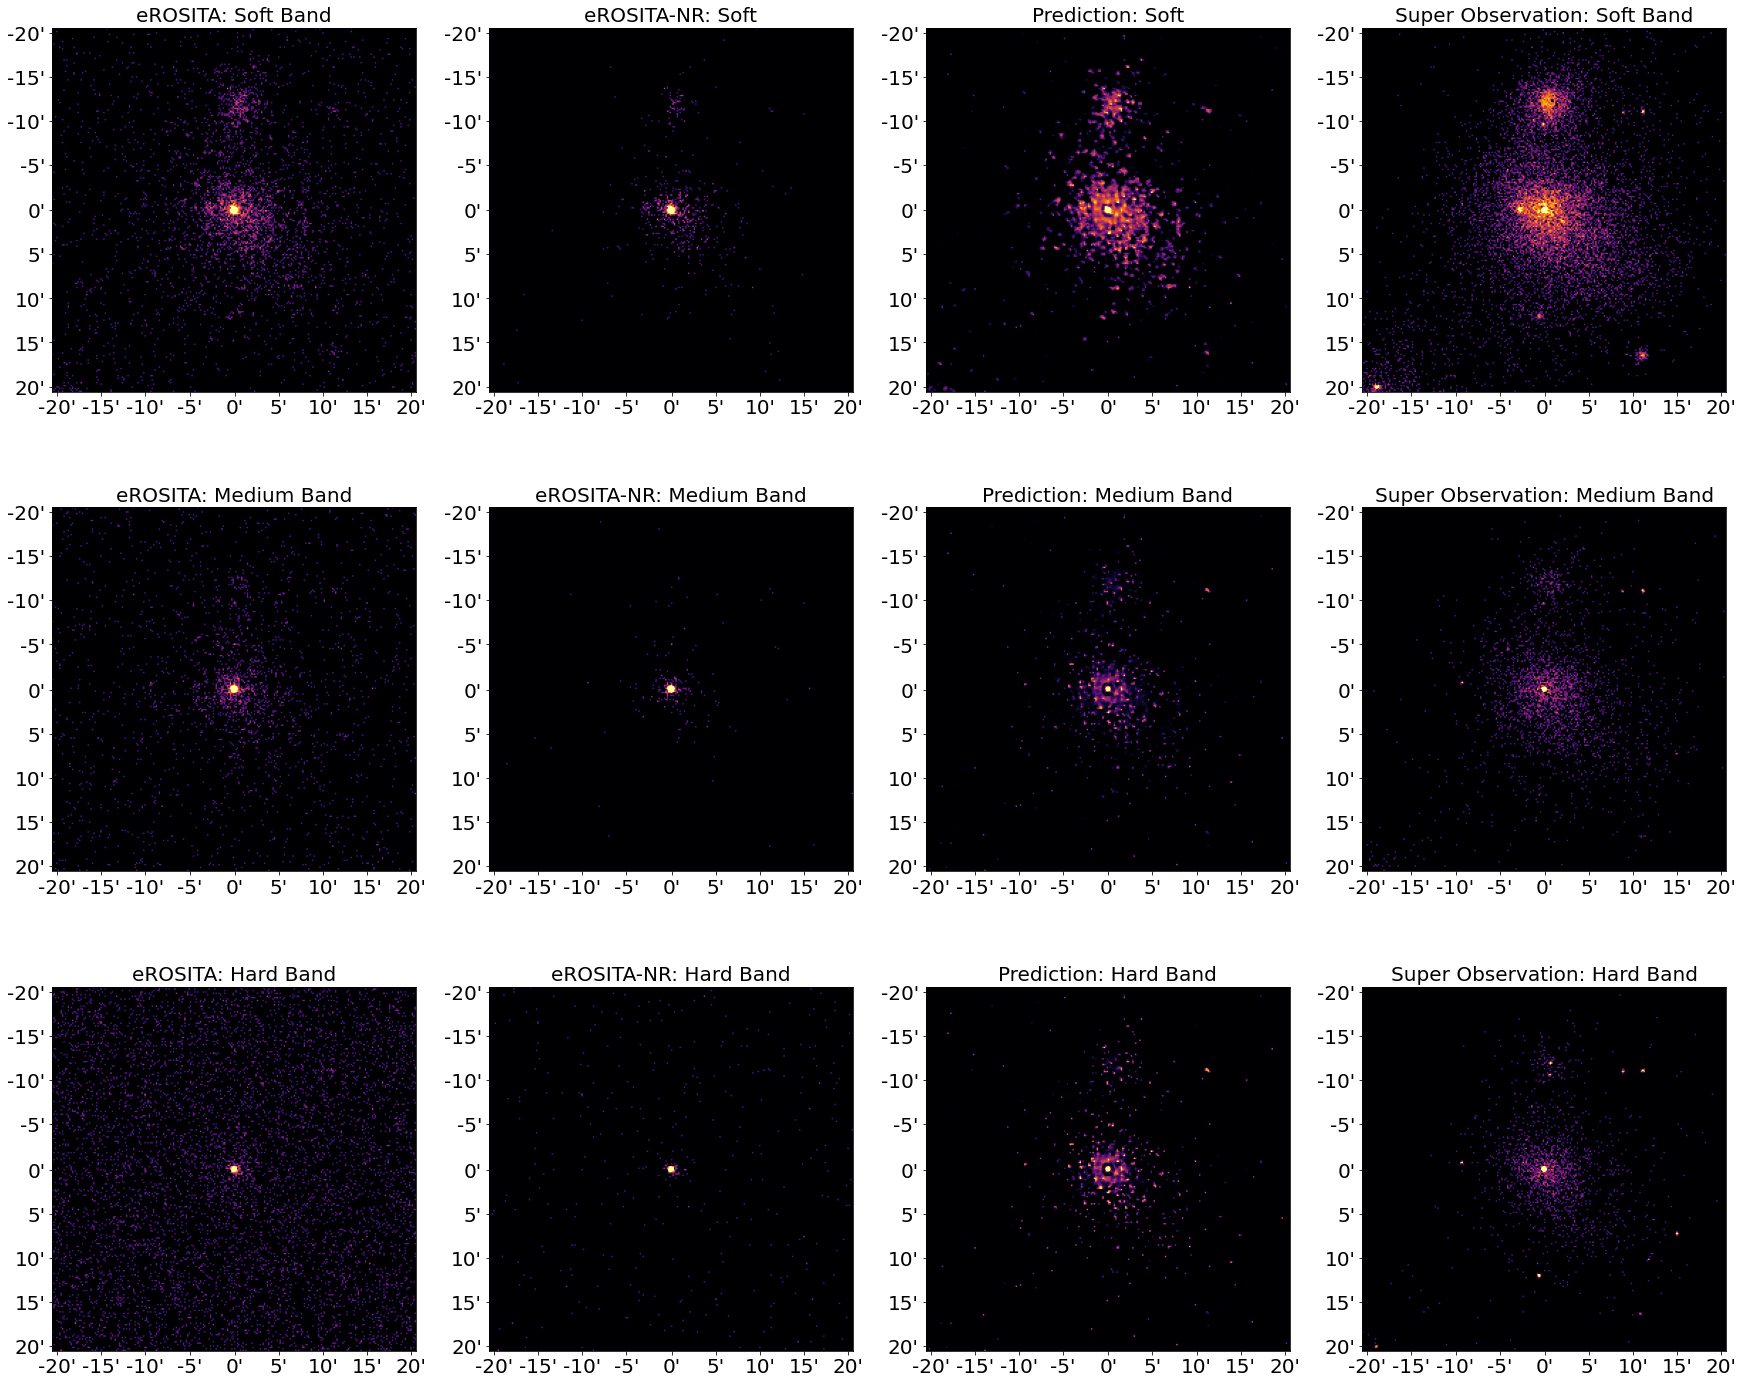
\includegraphics[width=\textwidth]{Ch2_Super_Obs/typical_cluster_example_tpm222_corrected_1skip_linear_output_070122_index_1509.png}
\end{figure*}
\begin{figure*}%[b]
    \centering
    \caption{\raggedright Example observations of a sample galaxy cluster. The cluster shown has $M_{500c}=8.2\times10^{13}M_{\odot}$ and is at $z=0.07$. Rows correspond to the soft, medium, and hard X-ray energy bands. Columns correspond to different observation types (see \S\ref{ch2_data}), from left to right:  the \textit{eROSITA} mock image used as the machine learning input (``eROSITA''), a background subtracted image (``eROSITA-NR''), the machine learning output (``Prediction''), and the ground truth long duration mock observation (``Super Observation''). The flux color mapping is in log space, with the same color scaling for each image, from a color minimum at 0 photons per pixel to a color maximum of 10 photons per pixel. The predictions of the machine learning method developed in this research visibly outperform the \textit{eROSITA} and background-subtracted \textit{eROSITA} observations.  While the soft band \textit{eROSITA} observation captures most of the shape of the central cluster and the merging cluster, the substructure of central cluster and the neighboring AGN are not obviously distinguishable. The soft band prediction, on the other hand, shows most of this information clearly. This superior performance is most visible in the hard band, where \textit{eROSITA} is less sensitive and more noisy. The hard band \textit{eROSITA} observation displays the core of the central cluster in a field of background emission, whereas the prediction clearly shows the full shape of the central and merging cluster. For a more quantitative comparison of the results, see Section \ref{ch2_results}.}
    \label{fig:example_results}
\end{figure*}

\subsection{Data}\label{ch2_data}
Machine learning methods, in combination with hydrodynamic cosmological simulations, offer a powerful tool for galaxy cluster science. Machine learning methods, especially the convolutional neural network variant we develop in \S\ref{algorithm}, are exceptional at learning complicated patterns in multi-dimensional data. The methods we use require ``labeled'' data, meaning we need many realistic observations of galaxy clusters paired with matching, longer duration, background-free observations, which we refer to as ``super observations.'' Moreover, the choice of data determines the utility of the algorithm, meaning we need realistic observations of accurately simulated clusters. We choose to use hydrodynamic cosmological simulations because they easily provide pairs of simulated \textit{eROSITA} observations and super observations, while also closely matching the observed properties of AGN and the ICM \cite[see e.g.,][]{Hirschmann_2014, Rasia_2015, magneticum}. 

This research requires a hydrodynamic cosmological simulation large enough to generate a diverse sample of clusters and also high enough resolution to accurately model cluster substructures. To satisfy these constraints, we use the hydrodynamic cosmological simulation \texttt{Magneticum} \cite{magneticum}. Specifically, we use Box2/hr \cite{Hirschmann_2014}, a 352 Mpc/h sized  box with $2 \times 1584^3$ particles. It has a dark matter particle mass $M_{DM} = 6.9\times10^{8} M_{\odot}$, gas particle mass $M_{gas}=1.4\times10^{8}M_{\odot}$, and provides 6927 clusters at redshift $z=0.07$ with masses above $10^{13}M_{\odot}$, with a variety of mass accretion histories. The simulation uses cosmology constraints from \cite{Komatsu_2011}; i.e., total matter energy density, $\Omega_M = 0.272$ with 16.8\% baryons, a cosmological constant, $\Omega_{\Lambda} = 0.728$, Hubble constant, $H_0 = 70.4$, spectral index of the primordial power spectrum, $n_{s} = 0.963$, and an amplitude of matter fluctuations, $\sigma_8 = 0.809$.

Machine learning algorithms are inherently data driven, and therefore careful consideration must be given to data selection. To avoid biasing our model towards the more plentiful low mass, low redshift, clusters, we chose a roughly uniform mass and redshift distribution of clusters. We did so by subsampling the available low mass, low redshift clusters. Each cluster is included in the data set only once, from a unique line of sight. Our data set has 3285 galaxy cluster observations. Observations have a depth of 10 Mpc, and include emission from the galaxy cluster, nearby neighboring galaxy clusters, and nearby AGN. The emission from AGN is simulated as detailed in \cite{Biffi_2018}. Observed galaxy clusters have a mass range of $3.16 \times 10^{13}$ $M_{\odot}$ to $1.17 \times 10^{15}$ $M_{\odot}$ and a redshift range of 0.07 to 0.47.

The goal of our work is to create an algorithm capable of predicting a high quality observation from a lower quality observation. To do so, we must train the algorithm using pairs of observations. The galaxy cluster observations are therefore split in two categories, mock \textit{eROSITA} observations and super observations. The mock \textit{eROSITA} observations begin with a field of view and resolution matching that of \textit{eROSITA}, with a field of view of roughly 1 degree and a pixel size of 9.6 arcseconds. The observation time of these images is 2 ks. Expected background particle emission, instrument response, and point spread function are simulated using the \texttt{SIXTE} software \cite{SIXTE}. The super observations have the same detector area, field of view, and resolution as the \textit{eROSITA} observations, but are background-free, lack any instrument response or point spread function, and have an observation time of 10 ks. Because our over-arching goal is to accurately predict follow-up observations including line-of-sight AGN sources, AGN sources within 10 Mpc of the central galaxy cluster are included in our super observations. 

A background-subtracted \textit{eROSITA} observation set, which we refer to as \textit{eROSITA}-NR, is used as a baseline to compare prediction effectiveness to a non-machine learning method. The per-pixel background is defined as the mean of all nonzero pixels in an annulus with an inner radius of 140 pixels and a width of 5 pixels. This annulus range is sufficiently large to be exterior to all of the clusters' $R_{500c}$ radii in our data set. This is important, because we use the $R_{500c}$ radius, which is the radius in which the mass density of the cluster is 500 times the critical density of the Universe, and as a measure of the extent of the cluster. After the subtraction, all pixels with flux values less than zero are set to zero.

Each observation is divided into three energy bands, corresponding to soft X-rays (0.5-1.2 keV), medium X-rays (1.2-2.0 keV), and hard X-rays (2.0-7.0 keV). These bands were chosen following the definitions of the \textit{Chandra}/ACIS science and source detection energy bands\footnote{https://cxc.harvard.edu/csc/columns/ebands.html}, and also to take advantage of the different spectral behavior of AGN, ICM, and \textit{eROSITA} particle background. The frequency of the photons is known exactly for super observations, but for mock \textit{eROSITA} observations photons are sorted by their observed \textit{eROSITA}-defined channel number (PHA channel). The soft, medium, and hard X-rays are divided by the PHA bands 74-177, 178-274, and 275-722 respectively. Due to memory constraints, we only used the inner 256$\times$256 pixels of each image. This reduces the field of view to 40.96 arcminutes, but leaves the resolution unchanged. A summary of the observation image information is shown in Table \ref{tab:image_facts}. An example cluster, seen via mock \textit{eROSITA}, \textit{eROSITA}-NR, prediction, and super observations, is shown in Figure \ref{fig:example_results}.


\begin{table*}[h!]
\centering
\setlength\tabcolsep{0pt}
 \begin{tabular*}{\linewidth}{@{\extracolsep{\fill}}||c| c c c c||} 
 \hline\hline
 Observation & Field of View & Pixel Size & Exposure Time & Background\\ [0.5ex]
  & & & & Soft/Med/Hard\\
  & (arcminutes) & (arcseconds) & (s)&
 (counts/pixel)\\ [0.5ex]
 \hline\hline
 \textit{eROSITA} &  40.96' & 9.6"$\times$9.6" & 2000& 0.02/0.02/0.1\\[1ex] 
 Super Observation &  40.96' & 9.6"$\times$9.6" & 10000& 0\\[1ex]
 \hline\hline
 \end{tabular*}
 \caption{\label{tab:image_facts} A table of the image information. All observations types have the same field of view and the same angular resolution. They differ only in observing time and background level. Super observations are ideal observations; long exposure time, background-free, perfect instrument response, and no point spread function. Background counts are estimates from simulated blank sky observations that were put through our pipeline.}
\end{table*}

\subsection{Algorithm}\label{algorithm}

Convolutional neural networks are a class of machine learning algorithm that are often used for image processing tasks.  They make use of what are called ``convolutional filters.'' In the two dimensional case these can be understood as two dimensional matrices, where each element of the matrix is a parameter fitted during training. Images are convolved by sliding these filters over the image, taking the dot product of the matrix and a given region of the image. The size of these filter matrices and the method of sliding them over an image are hyperparameters determined by the user. During training these filters transition from random realizations to relevant feature detectors, commonly detecting edges, textures, and other patterns. By stacking layers of these filters on top of each other, the algorithm becomes capable of detecting more complex large scale features, like faces or animals. See \cite{LeCun_2015} for a review of deep learning and CNN's.

Our model is engineered to focus on accurately probing multiple length scales simultaneously. The images in our data set contain three primary components: ICM, AGN, and background, all of which are limited in size to length scales smaller than the entirety of the image. These small characteristic length scales encouraged us to abandon more traditional algorithm architectures, like the \texttt{UNET} \cite{UNET}, which rely on reducing images into a small set of globally important features. Our model instead consists primarily of two layers split into three paths. Each path has different sized filters (1$\times$1, 3$\times$3, 5$\times$5), each with 200 filters. We constructed and trained our model using the \texttt{Python} \cite{Python3} module \texttt{Tensorflow} \cite{tensorflow2015-whitepaper}.

In the first layer, an input image observation is fed directly into each path. After having the filters applied to it, the image is compressed back into a 3-band image using 1$\times$1 filters, thus leaving us with three different 3-band images. These images are concatenated together to form a single 9-band image. This image is then also reduced into a 3-band image using 1$\times$1 filters. This composite 3-band image is then fed into another layer of the same structure as the first, albeit with differently trained weightings. The outputs of each of these paths in the second layer is then concatenated with the 3-band output of the corresponding path of the first layer. Filters are applied to these concatenations so that they are transformed into 3-band images. These three resulting 3-band images are then themselves, with the initial input, concatenated. The resulting 12-band image is then subsequently reduced to a 3-band image output. Our resulting model has 48,687 trainable parameters. A diagram of this algorithm is shown in Figure \ref{fig:Algorithm} and is described in Table \ref{tab:algorithm_breakdown}.

We chose these three different filter sizes to correspond to relevant image properties. Different astrophysical objects and features have different spatial and spectral properties, e.g. AGN flux is spatially compact and is brighter in hard X-ray while ICM flux is spatially correlated on larger scales and is dominant in soft X-ray. The 1$\times$1 filter path examines purely spectral information, comparing the ratio of the fluxes in each energy band, which we believe improves background suppression and AGN identification, as both of these image features have limited spatial correlations but unique spectral behaviors. The 3$\times$3 and 5$\times$5 filter paths then ought to identify spatial correlations from ICM, with two length scales chosen to account for both substructure and the varying pixel size of clusters given their mass distribution and redshift.

\begin{figure*}
    \centering
    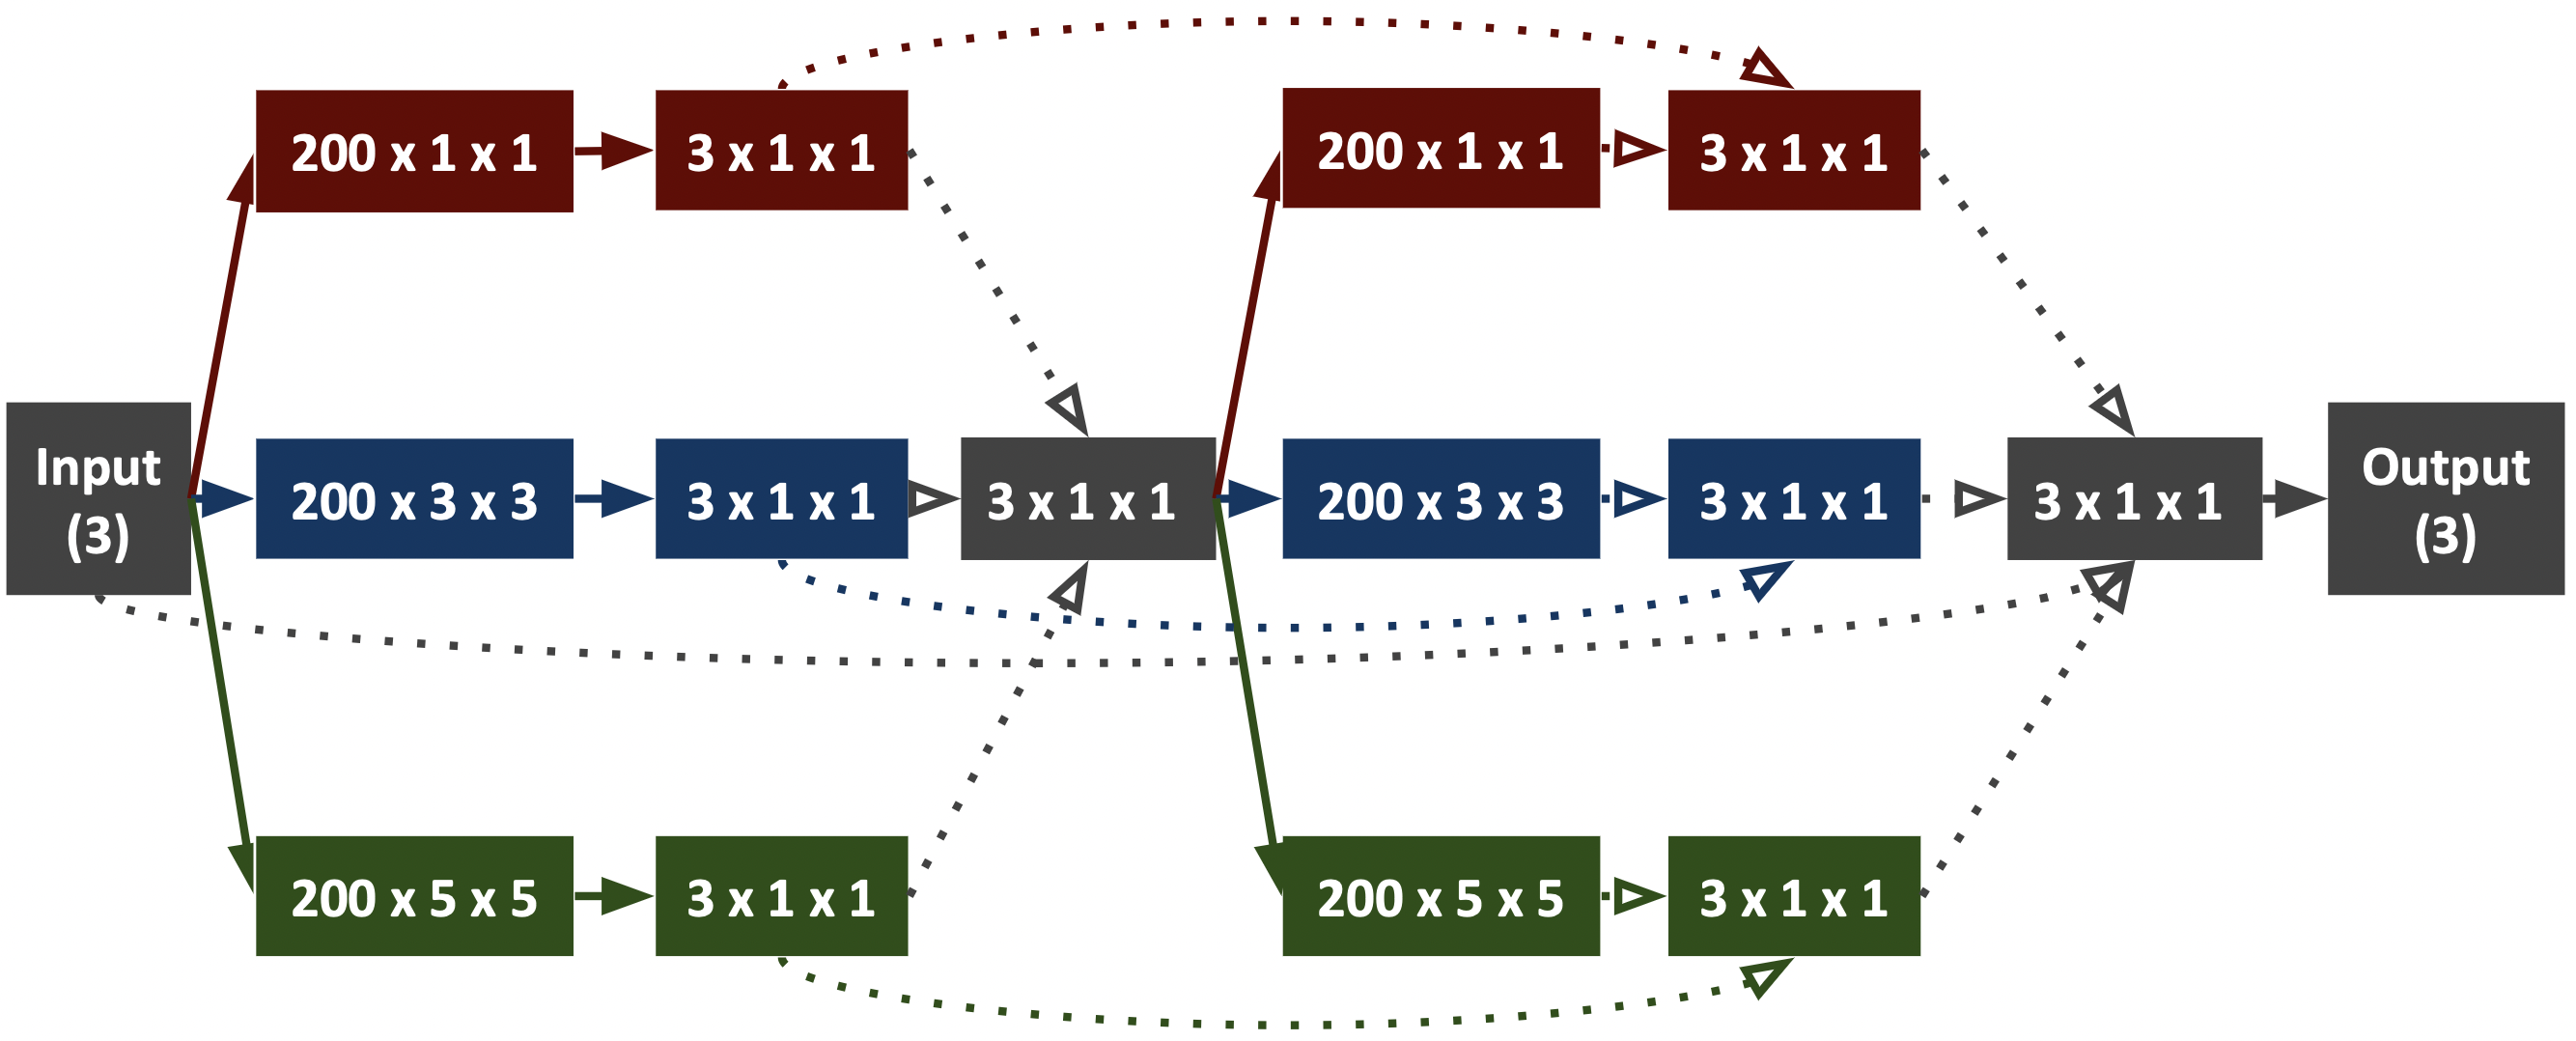
\includegraphics[width=\textwidth]{Ch2_Super_Obs/1skip.png}
    \caption{A diagram of the convolutional neural network architecture. We input a 256$\times$256 3-band pixel image. The three bands correspond to the three X-ray energy bands used, which were chosen to leverage both \textit{eROSITA}'s energy dependent sensitivity and the difference between AGN and ICM spectra. Further discussion of the energy bands is found in Section \ref{ch2_data}. The number of bands is shown in each box, either in parentheses or as the leftmost number. This is equal to the number of filters applied to the output of the preceding step (steps are linked by arrows). The three paths, each corresponding to a different filter size, are shown in different colors. Their filter sizes are the two rightmost numbers. From top to bottom the sizes of the filters in each path are 1$\times$1 (red), 3$\times$3 (blue), and 5$\times$5 (green). Dotted arrows indicate that a concatenation occurs before the filters are applied. This is done to probe different relevant length scales of an image without compressing the 256$\times$256 pixel size of the image. Instead, images are repeatedly reduced to 3-band images to reduce memory burden.}
\label{fig:Algorithm}
\end{figure*}

\begin{table*}%[h!]
\centering
\setlength\tabcolsep{0pt}
 \begin{tabular*}{\linewidth}{@{\extracolsep{\fill}}||c c c c c c||} 
 \hline
 Layer & Layer & Preceding & Filter & Kernel & Activation \\
 Name & Type & Layer(s) & \# & Size & \\ [0.5ex]
 \hline\hline
 x0 & Input & None & None & None & None \\ 
 x1 & Conv2D & x0 & 200 & 1$\times$1 & LeakyReLU\\
 x3 & Conv2D & x0 & 200 & 3$\times$3 & LeakyReLU\\
 x5 & Conv2D & x0 & 200 & 5$\times$5 & LeakyReLU\\
 x1b & Conv2DTranspose & x1 & 3 & 1$\times$1 & LeakyReLU\\ 
 x3b & Conv2DTranspose & x3 & 3 & 1$\times$1 & LeakyReLU\\
 x5b & Conv2DTranspose & x5 & 3 & 1$\times$1 & LeakyReLU\\
 x\_concat & Concat & x1b, x3b, x5b & None & None & None\\
 z0 & Conv2DTranspose & x\_concat & 3 & 1$\times$1 & LeakyReLU\\
 z1 & Conv2D & z0 & 200 & 1$\times$1 & LeakyReLU\\
 z3 & Conv2D & z0 & 200 & 3$\times$3 & LeakyReLU\\
 z5 & Conv2D & z0 & 200 & 5$\times$5 & LeakyReLU\\
 z1b & Concat & x1, z1 & None & None & None\\ 
 z3b & Concat & x3, z3 & None & None & None\\
 z5b & Concat & x5, z5 & None & None & None\\
 z1c & Conv2DTranspose & z1b & 3 & 1$\times$1 & LeakyReLU\\ 
 z3c & Conv2DTranspose & z3b & 3 & 1$\times$1 & LeakyReLU\\
 z5c & Conv2DTranspose & z5b & 3 & 1$\times$1 & LeakyReLU\\
 z\_concat & Concat & x0, z1c, z3c, z5c & None & None & None\\ 
 Output & Conv2DTranspose & z\_concat & 3 & 1$\times$1 & Linear\\[1ex] %Output (Conv2DTranspose)
 \hline
 \end{tabular*}
 \caption{\label{tab:algorithm_breakdown}A table of the convolutional neural network algorithm. A 256$\times$256 3-band pixel image is fed into the algorithm. Through an interconnected series of convolution and transpose convolution layers we achieve accurate predictions of cluster morphology while maintaining a smaller model. More details are available in Section \ref{algorithm} and Figure \ref{fig:Algorithm}.}
\end{table*}

\subsection{Training}\label{training}
Standard supervised machine learning training involves inputting data into an algorithm and then comparing the output (i.e., the prediction) to the label of the input (i.e., the truth value of the property of interest). The comparison is computed using a loss function. The weights of the algorithm are then changed to minimize the output of the loss function. In our case the inputs are the mock \textit{eROSITA} observations. The labels are the super observations. The loss function is a linear combination of the mean absolute error (i.e., the mean absolute difference between the pixels of the prediction image and the super observation)\footnote{We found that mean squared error performed poorly in the presence of background.} and ``morphology loss", defined as the linear combination of the mean absolute error of three morphology parameters; surface brightness concentration, asymmetry, and smoothness. We chose this loss function in order to emphasize the properties of the cluster we view as most important. By training minimizing the morphology loss of the algorithm, we improve the morphology parameters derived from predictions produced by the algorithm. We also tried a perceptual loss function, inspired by \cite{ploss}, using the third layer of the VGG19 network \cite{VGG19}. This is discussed in Section \ref{ch2_discussion}.

For the loss function we use ``fixed" versions of the morphology parameters, wherein either a fixed radius (in pixels) or the entire image is used to calculate the parameter. This is used in the algorithm because of its simplicity and consistency; it does not require information about the redshift or size of the central cluster. The fixed parameters are calculated as follows. The fixed surface brightness concentration is the ratio of the fluxes within 10 pixels and 100 pixels of the center of the image. The fixed asymmetry parameter is calculated using the absolute difference of the full image and the same image rotated 180 degrees, and is equal to the sum of the pixel values of this difference image normalized by the total flux of the original image. The fixed smoothness is calculated by applying an 11 pixel boxcar smoothing to the full original image, calculating the absolute difference between the smoothed image and the original image, summing the total flux of the difference image, and then normalizing that by the total flux of the original image. The fixed concentration, asymmetry, and smoothness parameters are described in equations \ref{fixed_c}, \ref{fixed_a}, and \ref{fixed_s}, respectively.  $\mathbf{X}$ is the observation image, $\mathbf{X_{180}}$ is the observation image rotated 180 degrees, $\mathbf{\tilde{X}}$ is the smoothed observation image, $F$ is the total flux with in some radius $r$ (if $r$ is unstated, the full image is used), where $r$ is in units of pixels. Examples of morphology parameter extremes, albeit for the $R_{500c}$ versions described in Section \ref{ch2_results}, are shown in Figure \ref{fig:morph_extremes}.

\begin{equation}\label{fixed_c}
    C = \frac{F(r \leq 10)}{F( r \leq 100)}
\end{equation}
\begin{equation}\label{fixed_a}
    A = \frac{F(|\mathbf{X}-\mathbf{X_{180}}|)}{F(\mathbf{X})}
\end{equation}
\begin{equation}\label{fixed_s}
    S = \frac{F(|\mathbf{X}-\mathbf{\tilde{X}}|)}{F(\mathbf{X})}
\end{equation}
Our training set, the data we set aside specifically for training the weights of the algorithm, constitutes 80\% of the full data set. 10\% of the remaining data forms our validation set. The validation set is used to evaluate the training progress in order to determine when to stop training. The algorithm is saved after each epoch it achieves a minimal validation loss. This procedure is repeated until the validation loss minimum is stable for over 100 epochs. The final 10\% of the data forms the test set, which is used to analyze the efficacy of the fully trained algorithm. The full data set is shuffled prior to partitioning.

\section{Results}\label{ch2_results}
Prediction algorithms like the one we are proposing must have clearly defined use cases. To illustrate the ways in which our model might benefit observers, we have defined several important predictive capabilities. These metrics are informed by the nature of the problem we seek to solve:  a follow-up observation of an initial \textit{eROSITA} observation will have higher signal to noise, a more physically accurate and more constrained luminosity profile, more visible substructure, and a more definite shape.  A prediction algorithm therefore must seek to increase the signal to noise in the input image, increase the brightness of astrophysical sources while differentiating between extended sources and point-spread-function-blurred AGN, and predict the location and brightness of real substructure. Similarly, the enhanced properties of the prediction must provide useful information for survey selection. That is why we chose to prioritize morphology parameters, which provide useful information about the properties of the cluster, especially those properties such as dynamical state, mass, and core type, which are of particular importance to galaxy cluster research. Note that while we prioritize morphologically accurate observations, we do not intend our prediction observations to be used for morphology measurements directly. Morphology is simply a metric we use to grade image accuracy (see Section \ref{ch2_discussion} for a discussion on assessing image accuracy and morphology).

Our intention is to aid in the selection of follow-up candidates, not to replace follow-up observations. Therefore, predictions must be probable enough to aid in discerning which clusters merit a follow-up. Metrics like those aforementioned provide an understanding for the accuracy of the predictions. An example prediction observation is shown in Figure \ref{fig:example_results}. Example observations of similar mass clusters with very different morphology parameters are shown in Figure \ref{fig:morph_extremes}. In the following subsections we examine the predicting power of our trained model for the three key morphology parameters (concentration \S\ref{concentration}, asymmetry \S\ref{asymmetry}, smoothness \S\ref{smoothness}), total flux (\S\ref{conserved flux}), and background reduction (\S\ref{background reduction}). We also evaluate the precision and accuracy of predictions as a function of mass (\S\ref{Mass Dependence}). We use the $R_{500c}$ versions of the morphology parameters. This formulation of the morphology parameters is more commonly used and more physically meaningful than the fixed version of the morphology parameters used in the loss function, but requires information about the cluster radius and redshift. Our true morphology parameters are calculated on observations with AGN, however the level of contamination from AGN in the soft band, where ICM dominates, is minimal.


\begin{figure*}%[b]
    \centering
    %\null \vspace{-20pt}
    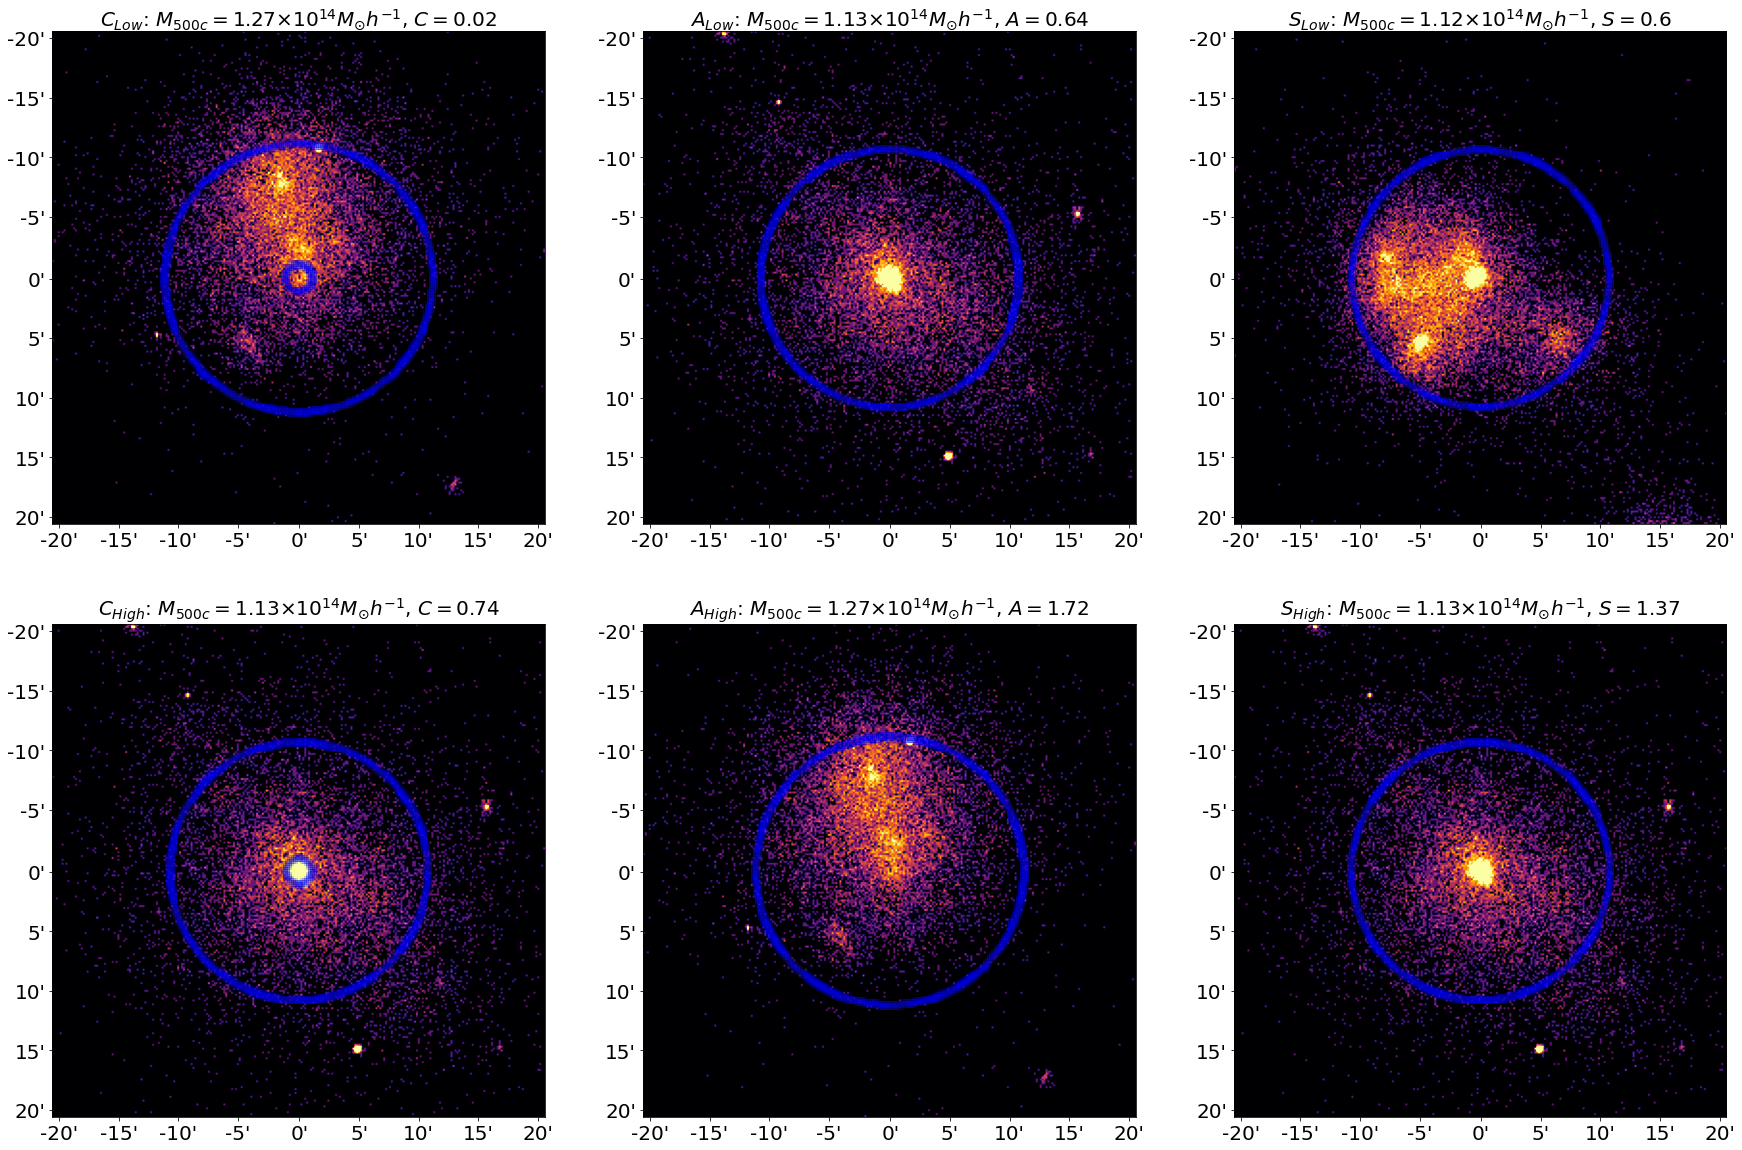
\includegraphics[width=\textwidth]{Ch2_Super_Obs/Morph_Extremes_tpm222_corrected_1skip_linear_output_060822.png}
    \caption{\raggedright Soft band observations of roughly equal mass clusters with varying $R_{500c}$ morphology parameters.  All clusters have a redshift of 0.07. Overlaid in blue is the $R_{500c}$ radius. For the leftmost column, the smaller blue circle is $.1\times R_{500c}$, which is used to calculate concentration.
    Left column:  An example of low (top) and high (bottom) concentration.
    Center column:  An example of low (top) and high (bottom) asymmetry.
    Right column:  An example of low valued (top) and high valued (bottom) smoothness. Larger values in the smoothness parameter indicate a peaky flux distribution. The bottom cluster is strongly concentrated (same cluster as bottom left) leading to higher smoothness value. The top cluster is clearly in a merger, which leads to a flatter flux distribution, meaning a more smoothly filled $R_{500c}$ radius.
    Note that the extremes in morphology parameter space tend to overlap, i.e., more centrally concentrated clusters tend to be more symmetric. For example, the same cluster is shown in the bottom left (highly concentrated) and top center (highly symmetric). Similarly, very asymmetric clusters tend to be less centrally concentrated. The top left cluster (less concentrated) and bottom center cluster (highly asymmetric) are the same.}
    \label{fig:morph_extremes}
\end{figure*}
\


\subsection{Concentration}\label{concentration}

Surface brightness concentration is a morphological parameter that estimates how centrally concentrated the mass of a galaxy cluster is, and is a key probe of a variety of cluster properties, including mass error \cite{Green_2019}, core type \cite{Santos_2008}, and dynamical state \cite{Rasia_2013, Parekh_2015, Lovisari_2017}. Given its ubiquity and usefulness as a metric, concentration is an important parameter for our prediction images to accurately replicate. Our $R_{500c}$ concentration parameter is modeled off the variant used by \cite{Lovisari_2017} and \cite{Green_2019}. The $R_{500c}$ surface brightness concentration calculates the ratio of the fluxes within $0.1 \times R_{500c}$ and within $R_{500c}$ of each cluster. Concentration varies from 0, a minimally concentrated cluster, to 1, a maximally concentrated cluster. Equation \ref{eqn_c}, shown below, describes the concentration calculation. Here $F$ denotes the total flux with in some pixel radius $r$.
\begin{equation}\label{eqn_c}
    C = \frac{F(r \leq .1 \times R_{500c})}{F( r \leq R_{500c})}
\end{equation}
True concentration is the concentration derived from the super observations.  We find that concentration values derived from the machine learning prediction observations are consistently closer to the true values, compared to concentrations derived from the \textit{eROSITA} or \textit{eROSITA}-NR images. In our test set data we find predicted $R_{500c}$ concentrations differed from the truth value by $(\Delta C_{\mathrm{soft}},\Delta C_{\mathrm{med}},\Delta C_{\mathrm{hard}}) = (0.02_{-0.04}^{+0.05}, 0.08_{-0.09}^{+0.1}, -0.03_{-0.1}^{+0.08})$, with the +/- values indicating the 84th and 16th percentile values in our test set results. Predicted soft band concentrations therefore have a roughly three times smaller median difference than the \textit{eROSITA} concentrations, with smaller scatter. This superiority is a reflection of the trained model's ability to simultaneously reduce background while boosting signal. This becomes especially apparent in the concentration parameters of the hard band, where high background dramatically degrades the accuracy. Here the median difference of prediction observation derived concentration is half that of the background subtracted \textit{eROSITA} concentration, the next most accurate concentration for that energy band, with half as much scatter. 

Plots of the concentration results as a function of the true (super observation) concentrations are shown in Figure \ref{fig:concentration}. In the top plots we show the median difference between the concentration derived by our prediction, the \textit{eROSITA} observation, or \textit{eROSITA}-NR observation and the super observation for the corresponding bins shown in the histograms directly below the plots. The shaded regions reflect the range of values in 68\% of the data in a given bin. The prediction-derived concentrations have a consistently lower bias and the results of the data have a consistently lower scatter across energy bands and true concentrations. Moreover, the bias and scatter of the concentration predictions are relatively consistent across true concentration bins, unlike the \textit{eROSITA}-derived results. Our results are evidence that a machine learning prediction model is better suited for accurately and precisely predicting concentrations of a diverse population of clusters than either the native \textit{eROSITA} observations or non-machine learning improvement. See Tables \ref{tab:training_v_test} and \ref{tab:training_v_test2} for a full quantitative comparison of the results.


\begin{figure*}%[b]
    \centering
    %\null \vspace{-20pt}
    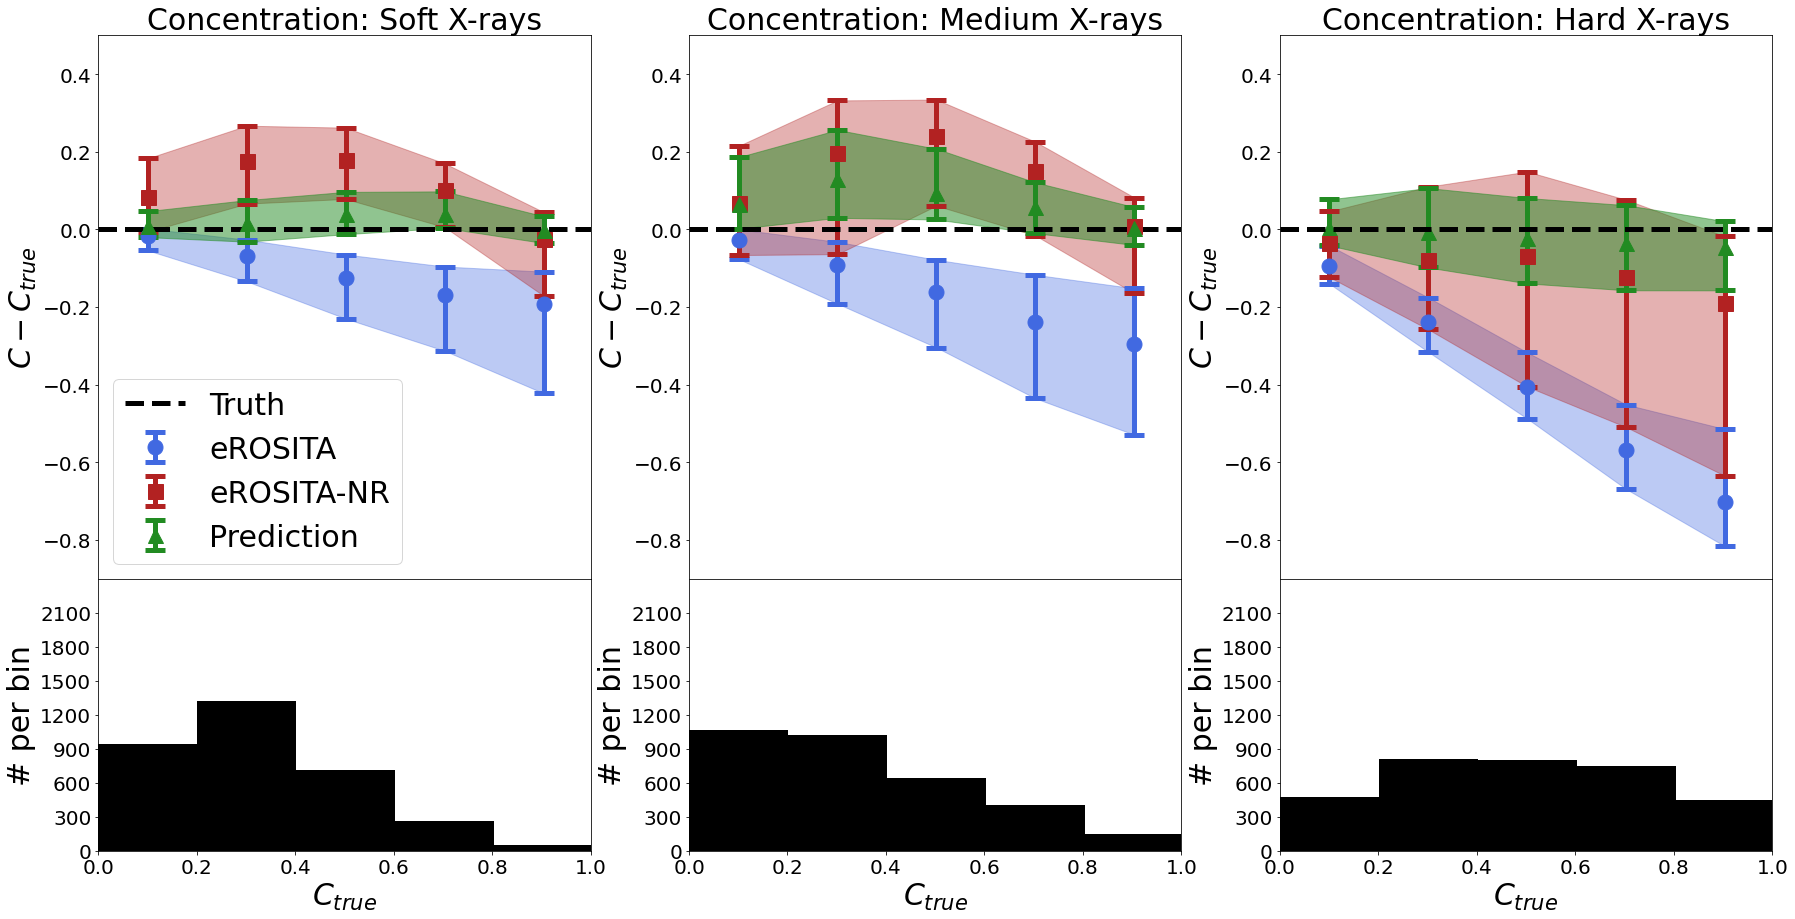
\includegraphics[width=\textwidth]{Ch2_Super_Obs/Concentration_Difference_Plots_tpm222_corrected_1skip_linear_output_062722.png}
    \caption{\raggedright $R_{500c}$ surface brightness concentration calculated for our full data set, as described in Section \ref{concentration}. The top plots show the difference between the calculated concentration from the \textit{eROSITA}, \textit{eROSITA}-NR (\textit{eROSITA} with background subtracted, see Section \ref{ch2_data}), and prediction observations each compared to the true concentration.  The true morphological parameters are calculated using the super observation. Results are binned by their true concentration value, with the number per bin shown in the histograms in the bottom panels. The median of the data in each bin (points) and the middle 68\% (error bars) are shown. For all energy bands, the prediction observation derived surface brightness concentrations are the most accurate. The median difference and scatter of those predictions appear to be independent of the true concentration, implying our prediction observations are valid for a diverse population of clusters.}
    \label{fig:concentration}
\end{figure*}

\subsection{Asymmetry}\label{asymmetry}
The asymmetry of a cluster, meaning its deviation from circularity in its two-dimensional profile, is another key morphological parameter. Several metrics have been devised to probe asymmetry, including ellipticity and photon asymmetry \cite[see][]{Ghirardini_2022}. Our $R_{500c}$ asymmetry metric is modeled off of the variants used by \cite{Rasia_2013} and \cite{Green_2019}. We choose this formulation because of its simple implementation, usefulness as a probe of cluster dynamical state \cite{Rasia_2013}, and informativeness in cluster mass estimation \cite{Green_2019}. Symmetric clusters are less likely to be disturbed, and thus estimations of their mass are probably less biased. Asymmetry is an obvious selection criteria for a variety of cosmological uses, therefore accurately predicting asymmetry is necessary for our model to be useful.%Asymmetry is, is also a useful parameter

The $R_{500c}$ asymmetry is calculated using the same procedure as the fixed asymmetry discussed in Section \ref{training}, but uses only pixels within $R_{500c}$. Asymmetry varies from 0, perfectly symmetric, to 2, maximally asymmetric. Equation \ref{eqn_a}, shown below, describes the calculation for asymmetry. Here $F$ denotes the total flux, $\mathbf{X}$ is the observation image, $\mathbf{X_{180}}$ is the observation image rotated 180 degrees, and $r$ is the radius within which the flux is calculated.

\begin{equation}\label{eqn_a}
    A = \frac{F(|\mathbf{X}-\mathbf{X_{180}}|;r\leq R_{500c})}{F(\mathbf{X};r\leq R_{500c})}
\end{equation}

Predicted asymmetry values are more closely correlated with super observation derived asymmetries than those from \textit{eROSITA} or \textit{eROSITA}-NR are. Asymmetry, compared to concentration, is poorly constrained in \textit{eROSITA} observations and is biased relative to super observation derived asymmetries. This is unsurprising, since asymmetry probes the less luminous outskirts of galaxy clusters, and is therefore more sensitive to background and short observation times. Despite this limitation, the prediction observation derived asymmetries are minimally biased across energy bands. In our test set data we found predicted $R_{500c}$ asymmetries differed from the truth value, as calculated using the super observations, by $(\Delta A_{\mathrm{soft}},\Delta A_{\mathrm{med}},\Delta A_{\mathrm{hard}}) = (0.03_{-0.12}^{+0.16}, -0.04_{-0.18}^{+0.16}, 0.06_{-0.24}^{+0.20})$. Like concentration, the strongest relative performance of the trained model's predictions for asymmetry is in the hard band. Here the median difference is $\sim6$ times smaller with comparable scatter compared to the \textit{eROSITA} results and $\sim4$ times smaller with nearly half as much scatter as the \textit{eROSITA}-NR results.  Plots of the asymmetry results as a function of the true (super observation) asymmetries are shown in Figure \ref{fig:asymmetry}. In the top plots we show the median difference between the super observation asymmetry and the asymmetry derived by our prediction, the \textit{eROSITA} observation, or \textit{eROSITA}-NR observation. The results are binned by the super observation derived asymmetry, with histograms of the bins shown directly below the plots. The shaded regions reflect the range of values in 68\% of the data in a given bin. Excluding the smallest asymmetry bin, which is too underpopulated to derive meaningful results, the bias in the asymmetry predictions is consistently lower than the other results. The asymmetry data set is not balanced across asymmetry parameter space, which is probably the cause of the slight dependence on true asymmetry. Very symmetric clusters are generally underrepresented in our data set, and therefore our model will struggle to accurately predict them. This could be corrected with access to more data. See Tables \ref{tab:training_v_test} and  \ref{tab:training_v_test2} for more quantitative information about the results.

\begin{figure*}%[b]
    \centering
    %\null \vspace{-20pt}
    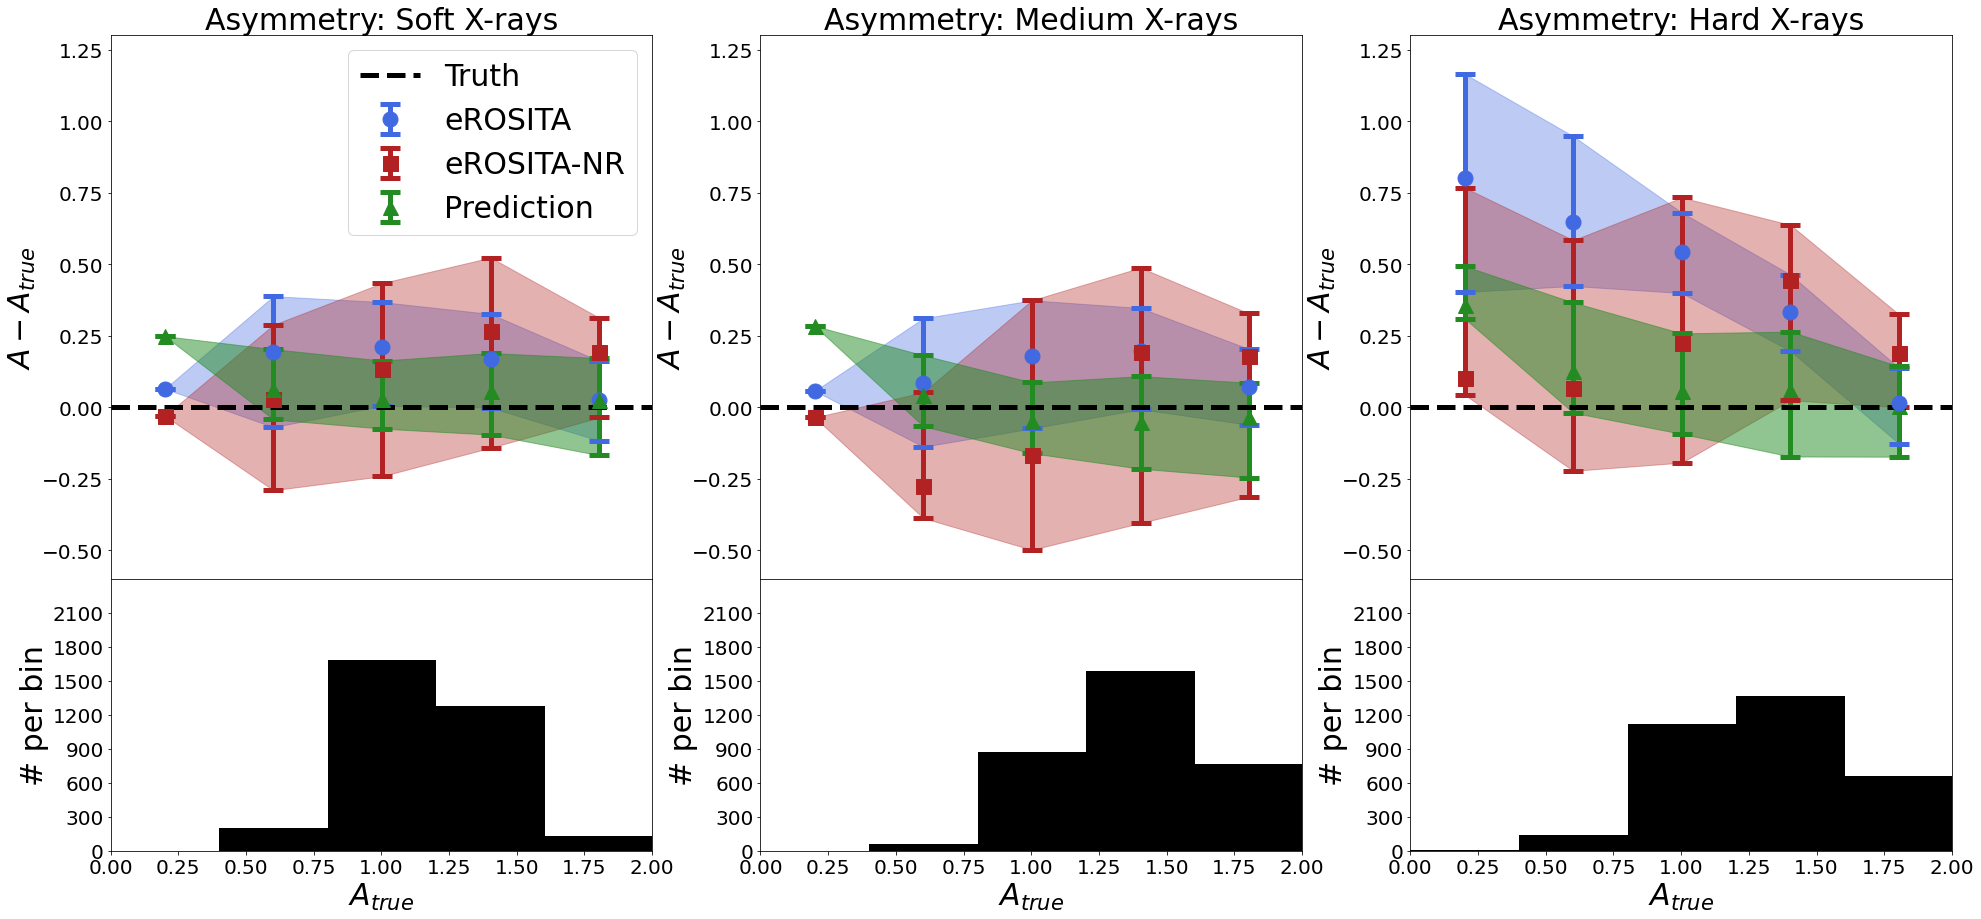
\includegraphics[width=\textwidth]{Ch2_Super_Obs/Asymmetry_Difference_Plots_tpm222_corrected_1skip_linear_output_072122.png}
    \caption{\raggedright Shown are plots of the $R_{500c}$ asymmetry calculated for our full data set, as described in Section \ref{asymmetry}. The top plots show the difference between the calculated asymmetry from the \textit{eROSITA}, \textit{eROSITA}-NR, and prediction observations and the true asymmetry, which is calculated using the super observation. Results are binned by their true asymmetry value, as shown in the histogram plots in the bottom row. The median of the data in each bin and the region representing 68\% of the results for the bins are plotted above. Prediction derived asymmetries are the most accurate, with lower median differences and much lower overall scatter. The median difference of asymmetry predictions appears to be dependent on true asymmetry, at least for low asymmetry clusters, suggesting the trained model overestimates the asymmetry of more circular clusters. The strength of this relationship is limited by the low number of highly symmetric clusters in our sample. Given the data-driven nature of machine learning algorithms, the limited number of highly symmetric clusters is probably the cause of the overestimation bias itself.}
    \label{fig:asymmetry}
\end{figure*}


\subsection{Smoothness}\label{smoothness}
As they grow, galaxy clusters accrete nearby dark matter and baryons. This process results in clumpy substructure within the cluster, which can be visible in X-ray observations. The smoothness morphology parameter is a measure of the amount of substructure in a galaxy cluster, which in turn provides information about the dynamical state of the cluster \cite{Rasia_2013}. Like the other morphology parameters, smoothness also provides important information for cluster mass estimation \cite{Green_2019}. We adopt the smoothness parameter as defined in \cite{Green_2019}, which is similar to the fluctuation parameter used in \cite{Rasia_2013}.

To calculate the $R_{500c}$ smoothness, like the fixed smoothness discussed in section \ref{training}, we again apply an 11 pixel boxcar smoothing scale, but only to the pixels within $R_{500c}$ of the center. Equation \ref{eqn_s}, shown below, describes the calculation for smoothness. Here $F$ denotes the total flux, $\mathbf{X}$ is the observation image, $\mathbf{\tilde{X}}$ is the observation image after boxcar smoothing has been applied, and $r$ is the radius within which the flux is calculated.

\begin{equation}\label{eqn_s}
    S = \frac{F(|\mathbf{X}-\mathbf{\tilde{X}}|;r\leq R_{500c})}{F(\mathbf{X};r\leq R_{500c})}
\end{equation}


As is the case with all the key morphology parameters, predicted smoothness values are more closely correlated with super observation derived smoothness than those from \textit{eROSITA} or \textit{eROSITA}-NR are. In our test set data we found predicted $R_{500c}$ smoothnesses differed from the truth value, as calculated using the super observations, by $(\Delta S_{\mathrm{soft}},\Delta S_{\mathrm{med}},\Delta S_{\mathrm{hard}}) = (0.03_{-0.06}^{+0.08}, -0.02_{-0.14}^{+0.1}, -0.03_{-0.08}^{+0.11})$. See Tables \ref{tab:training_v_test} and \ref{tab:training_v_test2} for more information.

Plots of the smoothness results as a function of the true (super observation) smoothness are shown in Figure \ref{fig:smoothness}. In the top plots we show the median difference between the smoothness derived by our prediction, the \textit{eROSITA} observation, or \textit{eROSITA}-NR observation and the super observation for the corresponding bins shown in the histograms directly below the plots. The shaded regions reflect the range of values in 68\% of the data in a given bin. The plots illustrate the prediction derived results low bias and low scatter in the data set across energy bands and smoothness parameter space. Like in the case of the asymmetry results, the strength of the results shown are limited by the unbalanced coverage of smoothness parameter space. Very smooth clusters, and very clumpy clusters in the soft X-ray, are not well represented. Machine learning is by nature data driven, so a lack of data in this parameter space could result in more inaccurate results.

\begin{figure*}%[b]
    \centering
    %\null \vspace{-20pt}
    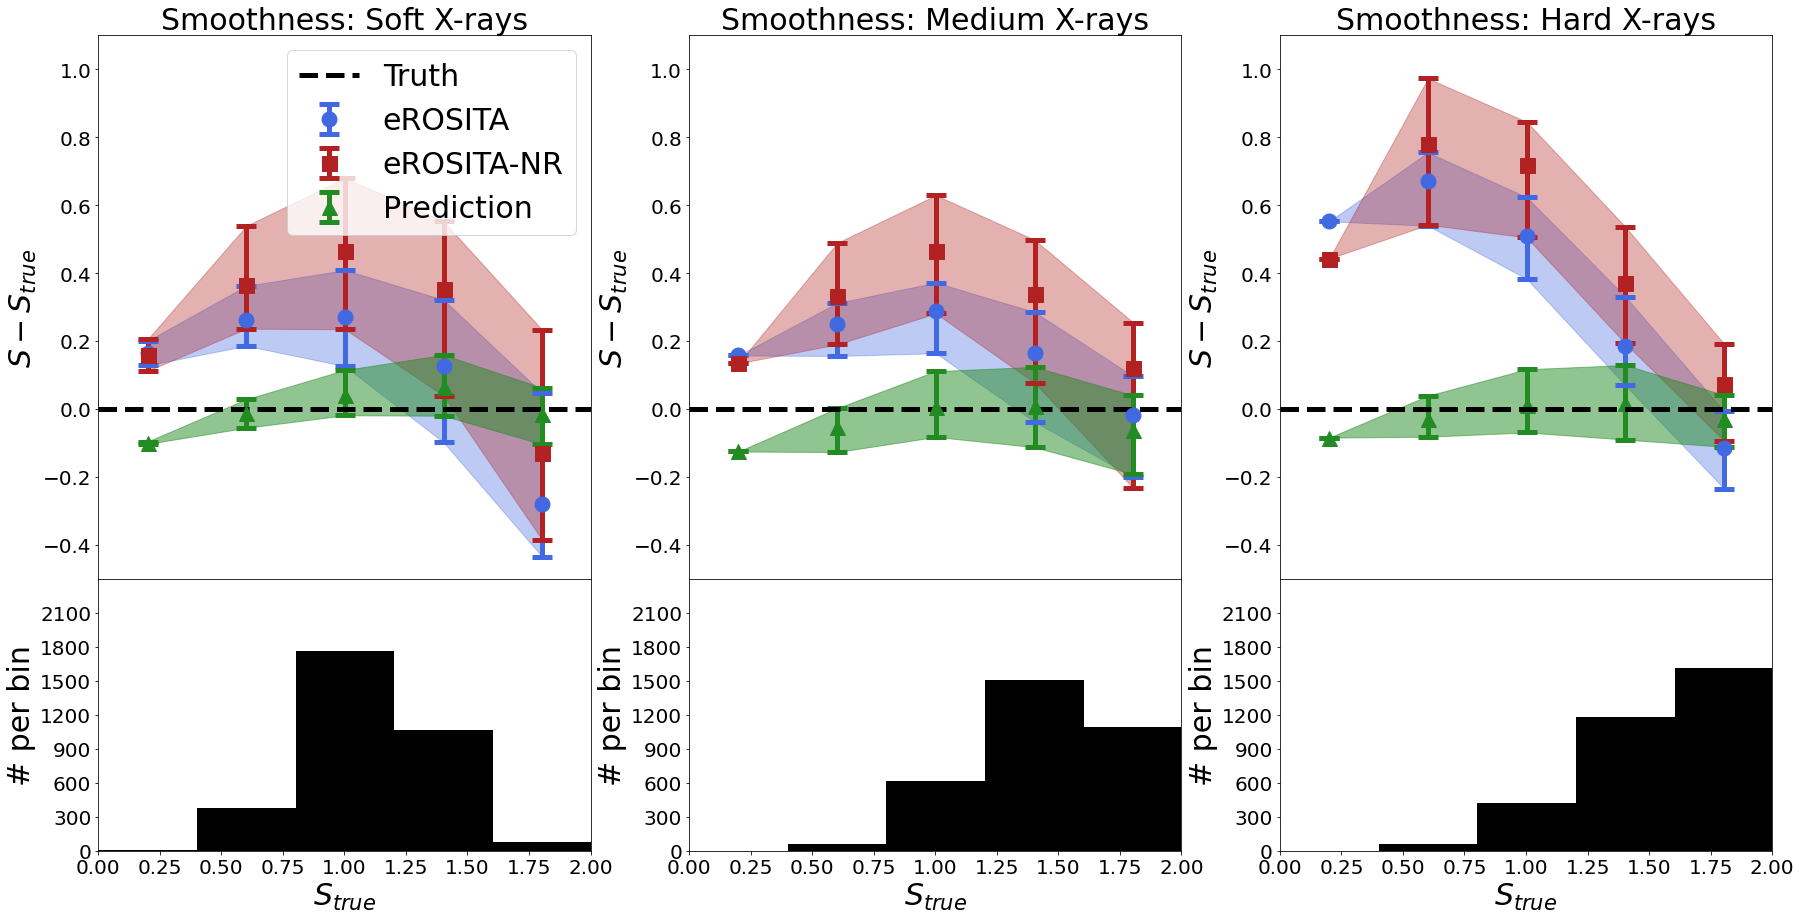
\includegraphics[width=\textwidth]{Ch2_Super_Obs/Smoothness_Difference_Plots_tpm222_corrected_1skip_linear_output_062722.png}
    \caption{\raggedright Plots of the $R_{500c}$ smoothness calculated for our full data set, as described in Section \ref{smoothness}. The top plots show the difference between the calculated smoothness from the \textit{eROSITA}, \textit{eROSITA}-NR, and prediction observations compared to the true smoothness, which is calculated using the super observation. Results are binned by their true smoothness value, as shown in the histogram plots in the bottom panels. The median of the data in each bin and the region representing 68\% of the results for the bins are plotted above. Of the morphology parameters calculated, smoothness is the most biased by low observation time, which is why \textit{eROSITA}-derived smoothness values differ so greatly from the true values. Low observation time increases the perceived clumpiness of the ICM because of Poisson sampling. Removing background via simple subtraction only exacerbates this bias by reducing the number of pixels observed to have photons from the ICM. The prediction model, which utilizes information about the full image smoothness, more effectively removes background while preserving signal, which is why it so strongly outperforms the other observation types in terms of accuracy. As with asymmetry, the distribution of true smoothness parameters is not uniform over the possible space, so one must use this machine learning method with care. Predictions of very smooth clusters, and very clumpy soft band clusters, are more likely to biased.}
    \label{fig:smoothness}
\end{figure*}

\subsection{Total Flux}\label{conserved flux}

Do prediction observations conserve the total flux of the observation? Because morphology parameters all involve normalization by the total flux, they shed little light on that question. Conservation of the total flux is a potentially important feature for prediction observations, however, and merits investigating. We perform a simple test of this and find that the prediction observations do preserve the flux, and do so with less scatter than the background-subtracted \textit{eROSITA} observations. See Figure \ref{fig:flux} for a plot of the results. Figure \ref{fig:flux} illustrates the power of our model in conserving total flux, especially with regards to the soft band, where the scatter in the difference between predicted and true total flux is negligible. The results are also listed in Tables \ref{tab:training_v_test} \ref{tab:training_v_test2}.

\begin{table*}[h!]
\centering
\setlength\tabcolsep{0pt}
 \begin{tabular*}{\linewidth}{@{\extracolsep{\fill}}||c c c c c c c||} 
 \hline\hline
  &  &  &  &  & & \\
 Observation & Band & C & A & S & F & B\\ [0.5ex] 
 \hline\hline
 Training + Validation &  &  &  &  & & \\
 \hline\hline
 \textit{eROSITA} & Soft & $-0.07_{-0.1}^{+0.05}$ & $0.19_{-0.19}^{+0.17}$ & $0.23_{-0.2}^{+0.15}$ & $0.72_{-0.08}^{+0.45}$& $1115_{-369}^{+74}$ \\[1ex] 
 \textit{eROSITA}-NR & Soft & $0.14_{-0.12}^{+0.1}$ & $0.18_{-0.4}^{+0.29}$ & $0.41_{-0.25}^{+0.22}$ & $-0.06_{-0.18}^{+0.04}$& $10_{-4}^{+4}$ \\[1ex]
 Prediction & Soft & $0.02_{-0.04}^{+0.06}$ & $0.04_{-0.12}^{+0.13}$ & $0.04_{-0.07}^{+0.09}$ & $-0.06_{-0.26}^{+0.05}$& $138_{-37}^{+19}$ \\[1ex]
 \hline
 \textit{eROSITA} & Medium & $-0.09_{-0.15}^{+0.07}$ & $0.16_{-0.21}^{+0.17}$ & $0.12_{-0.2}^{+0.17}$ & $0.71_{-0.05}^{+0.27}$& $1222_{-179}^{+54}$ \\[1ex] 
 \textit{eROSITA}-NR & Medium & $0.14_{-0.2}^{+0.15}$ & $0.12_{-0.56}^{+0.31}$ & $0.27_{-0.25}^{+0.22}$ & $-0.01_{-0.04}^{+0.02}$& $11_{-3}^{+4}$ \\[1ex]
 Prediction & Medium & $0.08_{-0.08}^{+0.13}$ & $-0.04_{-0.15}^{+0.14}$ & $-0.02_{-0.12}^{+0.11}$ & $0.0_{-0.05}^{+0.01}$& $100_{-15}^{+15}$ \\[1ex]
 \hline
 \textit{eROSITA} & Hard & $-0.38_{-0.25}^{+0.22}$ & $0.37_{-0.3}^{+0.21}$ & $0.04_{-0.21}^{+0.33}$ & $3.41_{-0.11}^{+0.06}$& $6530_{-789}^{+193}$ \\[1ex] 
 \textit{eROSITA}-NR & Hard & $-0.09_{-0.27}^{+0.18}$ & $0.29_{-0.37}^{+0.33}$ & $0.22_{-0.22}^{+0.34}$ & $0.1_{-0.21}^{+0.04}$& $311_{-39}^{+22}$ \\[1ex]
 Prediction & Hard & $-0.02_{-0.11}^{+0.09}$ & $0.05_{-0.17}^{+0.18}$ & $-0.01_{-0.09}^{+0.1}$ & $0.01_{-0.04}^{+0.01}$& $152_{-24}^{+27}$ \\[1ex]
 \hline
 \end{tabular*}
 \caption{\label{tab:training_v_test} A table of the median and 68\% intervals for the difference between the \textit{eROSITA}/\textit{eROSITA}-NR/Prediction derived values and the super observation derived values for morphology parameters concentration (C), asymmetry (A), smoothness (S), total flux (F), and background removal (B). See Section \ref{ch2_results} for a description of each evaluation metric. See Section \ref{ch2_data} for information about the observation types and energy bands. Results for just the training and validation sets are shown (Table 3 in \cite{Soltis_2022} has been split in two). Prediction derived results for the test set are consistent with those from the training-validation combined data set, suggesting the trained model has not over-fit the training data.}
\end{table*}

\begin{table*}[h!]
\centering
\setlength\tabcolsep{0pt}
 \begin{tabular*}{\linewidth}{@{\extracolsep{\fill}}||c c c c c c c||} 
 \hline\hline
  &  &  &  &  & & \\
 Observation & Band & C & A & S & F & B\\ [0.5ex] 
 \hline\hline
 Test Data  &  &  &  &  &  &\\
 \hline\hline
  \textit{eROSITA} & Soft & $-0.07_{-0.09}^{+0.05}$ & $0.17_{-0.2}^{+0.17}$& $0.22_{-0.22}^{+0.15}$ & $0.72_{-0.08}^{+0.49}$& $1107_{-348}^{+78}$ \\[1ex] 
 \textit{eROSITA}-NR & Soft & $0.14_{-0.1}^{+0.1}$ & $0.16_{-0.39}^{+0.32}$ & $0.39_{-0.26}^{+0.24}$ & $-0.07_{-0.18}^{+0.04}$& $10_{-4}^{+4}$ \\[1ex]
 Prediction & Soft & $0.02_{-0.04}^{+0.05}$ & $0.03_{-0.12}^{+0.16}$ & $0.03_{-0.06}^{+0.08}$ & $-0.07_{-0.27}^{+0.05}$& $137_{-36}^{+19}$ \\[1ex]
 \hline
 \textit{eROSITA} & Medium & $-0.09_{-0.14}^{+0.07}$ & $0.17_{-0.22}^{+0.17}$ & $0.12_{-0.21}^{+0.17}$ & $0.71_{-0.06}^{+0.29}$& $1216_{-194}^{+58}$ \\[1ex] 
 \textit{eROSITA}-NR & Medium & $0.14_{-0.21}^{+0.15}$ & $0.13_{-0.58}^{+0.29}$ & $0.25_{-0.24}^{+0.27}$ & $-0.01_{-0.05}^{+0.02}$& $12_{-4}^{+3}$ \\[1ex]
 Prediction & Medium & $0.08_{-0.09}^{+0.1}$ & $-0.04_{-0.18}^{+0.16}$ & $-0.02_{-0.14}^{+0.1}$ & $0.0_{-0.05}^{+0.01}$& $100_{-15}^{+15}$ \\[1ex]
 \hline
 \textit{eROSITA} & Hard & $-0.37_{-0.26}^{+0.2}$ & $0.37_{-0.3}^{+0.23}$ & $0.02_{-0.2}^{+0.39}$ & $3.4_{-0.13}^{+0.06}$& $6519_{-802}^{+209}$\\[1ex] 
 \textit{eROSITA}-NR & Hard & $-0.07_{-0.23}^{+0.15}$ & $0.26_{-0.34}^{+0.38}$ & $0.21_{-0.24}^{+0.39}$ & $0.09_{-0.23}^{+0.05}$& $307_{-37}^{+24}$ \\[1ex]
 Prediction & Hard & $-0.03_{-0.1}^{+0.08}$ & $0.06_{-0.24}^{+0.2}$ & $-0.03_{-0.08}^{+0.11}$ & $0.0_{-0.06}^{+0.01}$& $151_{-19}^{+24}$ \\[1ex]
 \hline
 \end{tabular*}
 \caption{\label{tab:training_v_test2} A table of the median and 68\% intervals for the difference between the \textit{eROSITA}/\textit{eROSITA}-NR/Prediction derived values and the super observation derived values for morphology parameters concentration (C), asymmetry (A), smoothness (S), total flux (F), and background removal (B). See Section \ref{ch2_results} for a description of each evaluation metric. See Section \ref{ch2_data} for information about the observation types and energy bands. Results for just the test set are shown (Table 3 in \cite{Soltis_2022} has been split in two). Prediction derived results for the test set are consistent with those from the training-validation combined data set, suggesting the trained model has not over-fit the training data.}
\end{table*}

\begin{figure*}%[b]
    \centering
    %\null \vspace{-20pt}
    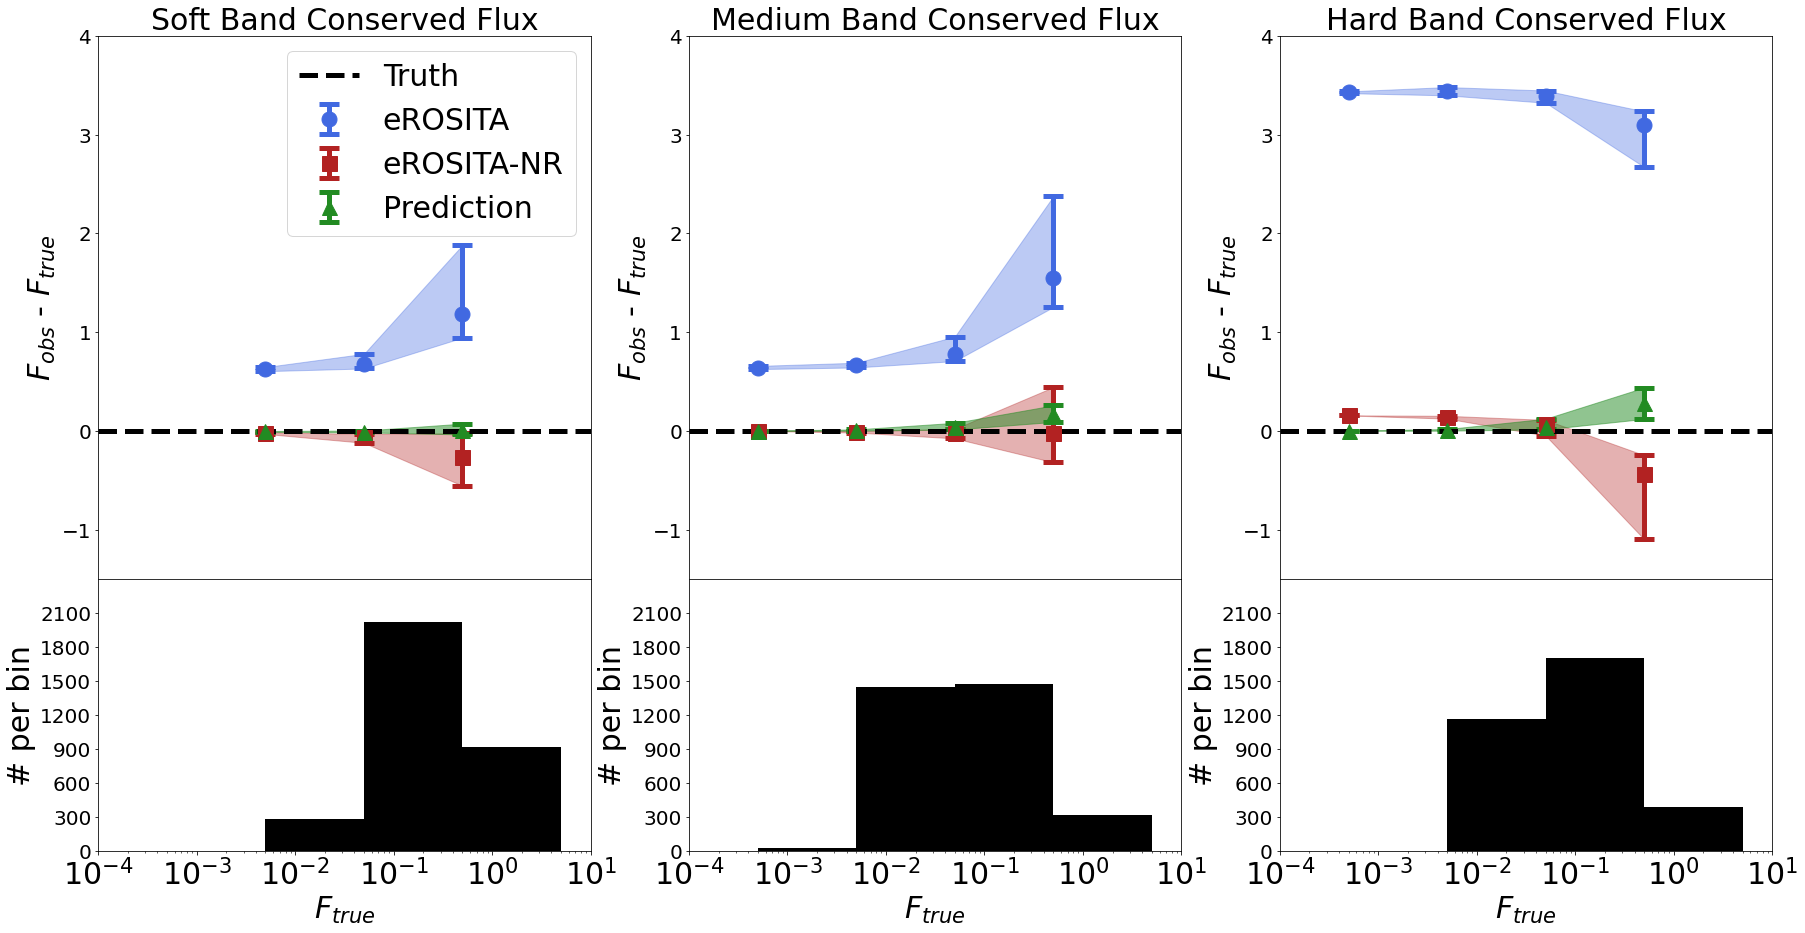
\includegraphics[width=\textwidth]{Ch2_Super_Obs/Conserved_Flux_Comparison_binned_062722.png}
    \caption{\raggedright Total flux for each observation. The format of the plots is the same as those of the morphology parameters. Total flux is defined as the total photon counts in an image normalized by the observing time. For the \textit{eROSITA} (plotted on the y-axis, shown in blue) and \textit{eROSITA}-NR  (plotted on the y-axis, shown in red) observations, this means a normalization of 2000 seconds. For the super observations (plotted on the x-axis), this is a 10,000 second normalization. The prediction observations (on the y-axis, shown in green) are also treated as 10,000 second observations. Results are binned by the true total flux, as determined by the super observation. A histogram of the bins used for the corresponding energy band is shown in each bottom panel. The prediction observations better preserve total flux than the \textit{eROSITA} or \textit{eROSITA}-NR observations. In the case of all of the \textit{eROSITA} observations and the \textit{eROSITA}-NR hard band observations this is because background photons dominate the image for dim sources. Even when \textit{eROSITA}-NR observations preserve the total flux decently well, as in the soft and medium energy bands, the prediction observations outperform them by maintaining a lower scatter.\newline}
    \label{fig:flux}
\end{figure*}

\subsection{Background Reduction}\label{background reduction}
Observations of galaxy clusters, like all astronomical observations, are hindered by various forms of background. Background in an observation has multiple sources. Background is generated both by non-galaxy cluster X-ray sources, particles, and as a product of the instrument itself. One potential use of an observation prediction model is to reduce background wherever possible. The machine learning model can achieve this by utilizing multi-wavelength information, as the cluster signal-to-background ratio of \textit{eROSITA} is higher at lower frequencies. Additionally, as the model learns the general shape of galaxy clusters and AGN it can better suppress pixels that do not conform to their luminosity profiles. It is important to reiterate that what the model produces is only a prediction and some background reduction will be inaccurate.

We can quantify background reduction by comparing our background-free super observations to our \textit{eROSITA}-like input observations and the prediction observations. We apply a Gaussian smoothing filter to the super observations in order to mimic the effects of both the point-spread function and the difference in the random realization of photons between observations. We then catalogue the pixels with zero flux in the smoothed images. For the rest of our observations, we define the background as the total flux of those pixels. Plots of the background results are shown in Figure \ref{fig:noise}. Tables \ref{tab:training_v_test} and \ref{tab:training_v_test2} quantify the results. 
We find that a background subtraction, as described in Section \ref{ch2_data}, outperforms our model's background suppression in the soft and medium energy bands. It does so at a cost to the accuracy in the $R_{500c}$ morphology parameters, especially asymmetry and smoothness (see Figures \ref{fig:asymmetry} and \ref{fig:smoothness}). The model outperforms subtraction in the hard energy band, however, where \textit{eROSITA} observations are especially background dominated. This advantage in performance could be useful for observations that are reliant on the hard band, like AGN-focused observations. Note that our mock \textit{eROSITA} observations only included simulated particle background, not X-ray foreground, or other X-ray background sources.

\begin{figure*}%[b]
    \centering
    %\null \vspace{-20pt}
    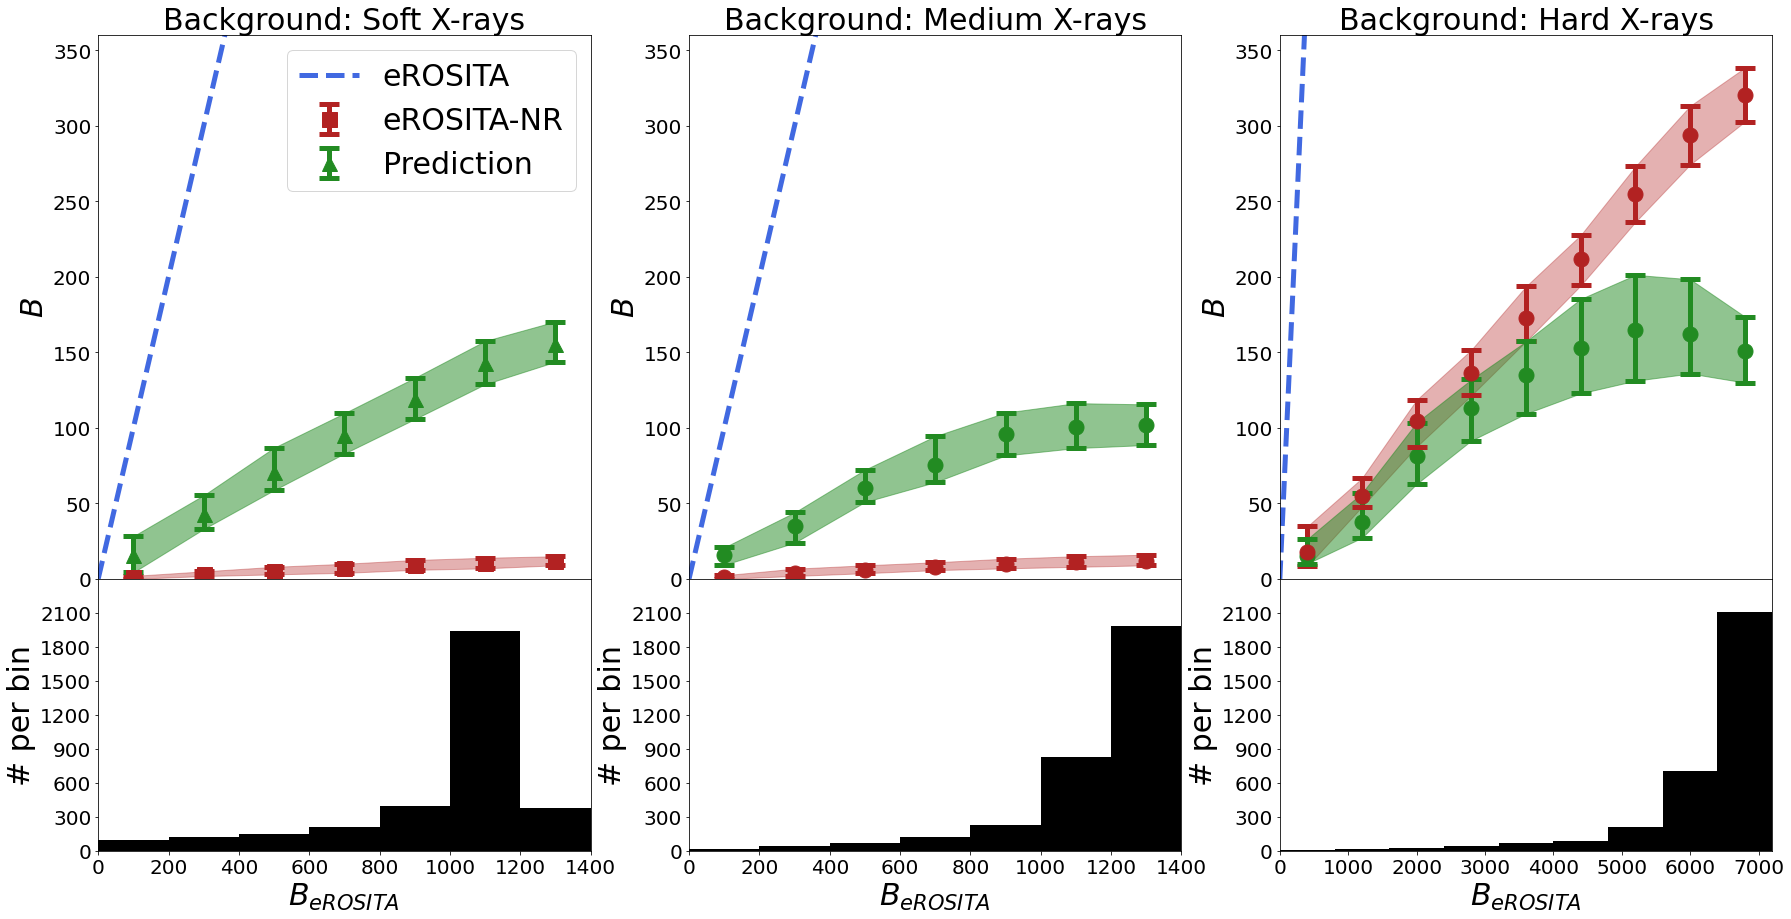
\includegraphics[width=\textwidth]{Ch2_Super_Obs/Background_Difference_Plot_tpm222_corrected_1skip_linear_output_072122.png}
    \caption{\raggedright Background calculated for our full data set, as described in Section \ref{background reduction}. The top plots show the background ($B$) from the \textit{eROSITA}, \textit{eROSITA}-NR, and prediction observations plotted against the \textit{eROSITA} observations background ($B_{eROSITA}$). Results are binned by their \textit{eROSITA} background, as shown in the histograms plots on the bottom. The median of the data in each bin and the region representing 68\% of the results for the bins are plotted above. The background subtraction method, described in Section \ref{ch2_data}, outperforms the prediction in background reduction for the soft and medium energy bands. The prediction observations have lower background in the hard band, however, likely due to the weak signal in \textit{eROSITA} observations at energies above 2 keV. Moreover, the prediction observations have the benefit of consistent background across energy bands, with only a weak dependence on the input observation's background. It should also be noted that the background subtraction method, while better at reducing background, also removes signal, and has worse morphology parameter accuracy.}
    \label{fig:noise}
\end{figure*}


\subsection{Mass Dependence}\label{Mass Dependence}
In addition to checking for bias in our prediction observations' morphological accuracy as a function of true morphology, we also examined whether there was any trend as a function of cluster mass. We found no obvious mass dependence in the soft band, which is the band most useful for measuring cluster morphology. The trends apparent in higher energy bands were very small, and the scatter in the difference between true and predicted parameters was roughly consistent across energy bands. These results suggest that the model predicts morphologically accurate and precise observations for clusters within our data sets mass range (i.e., $\sim 10^{13}$ to $10^{15} M_{\odot}$). See Figure \ref{fig:mass_dep} for a visualization of the results.

\begin{figure*}
    \centering
    %\null \vspace{-20pt}
    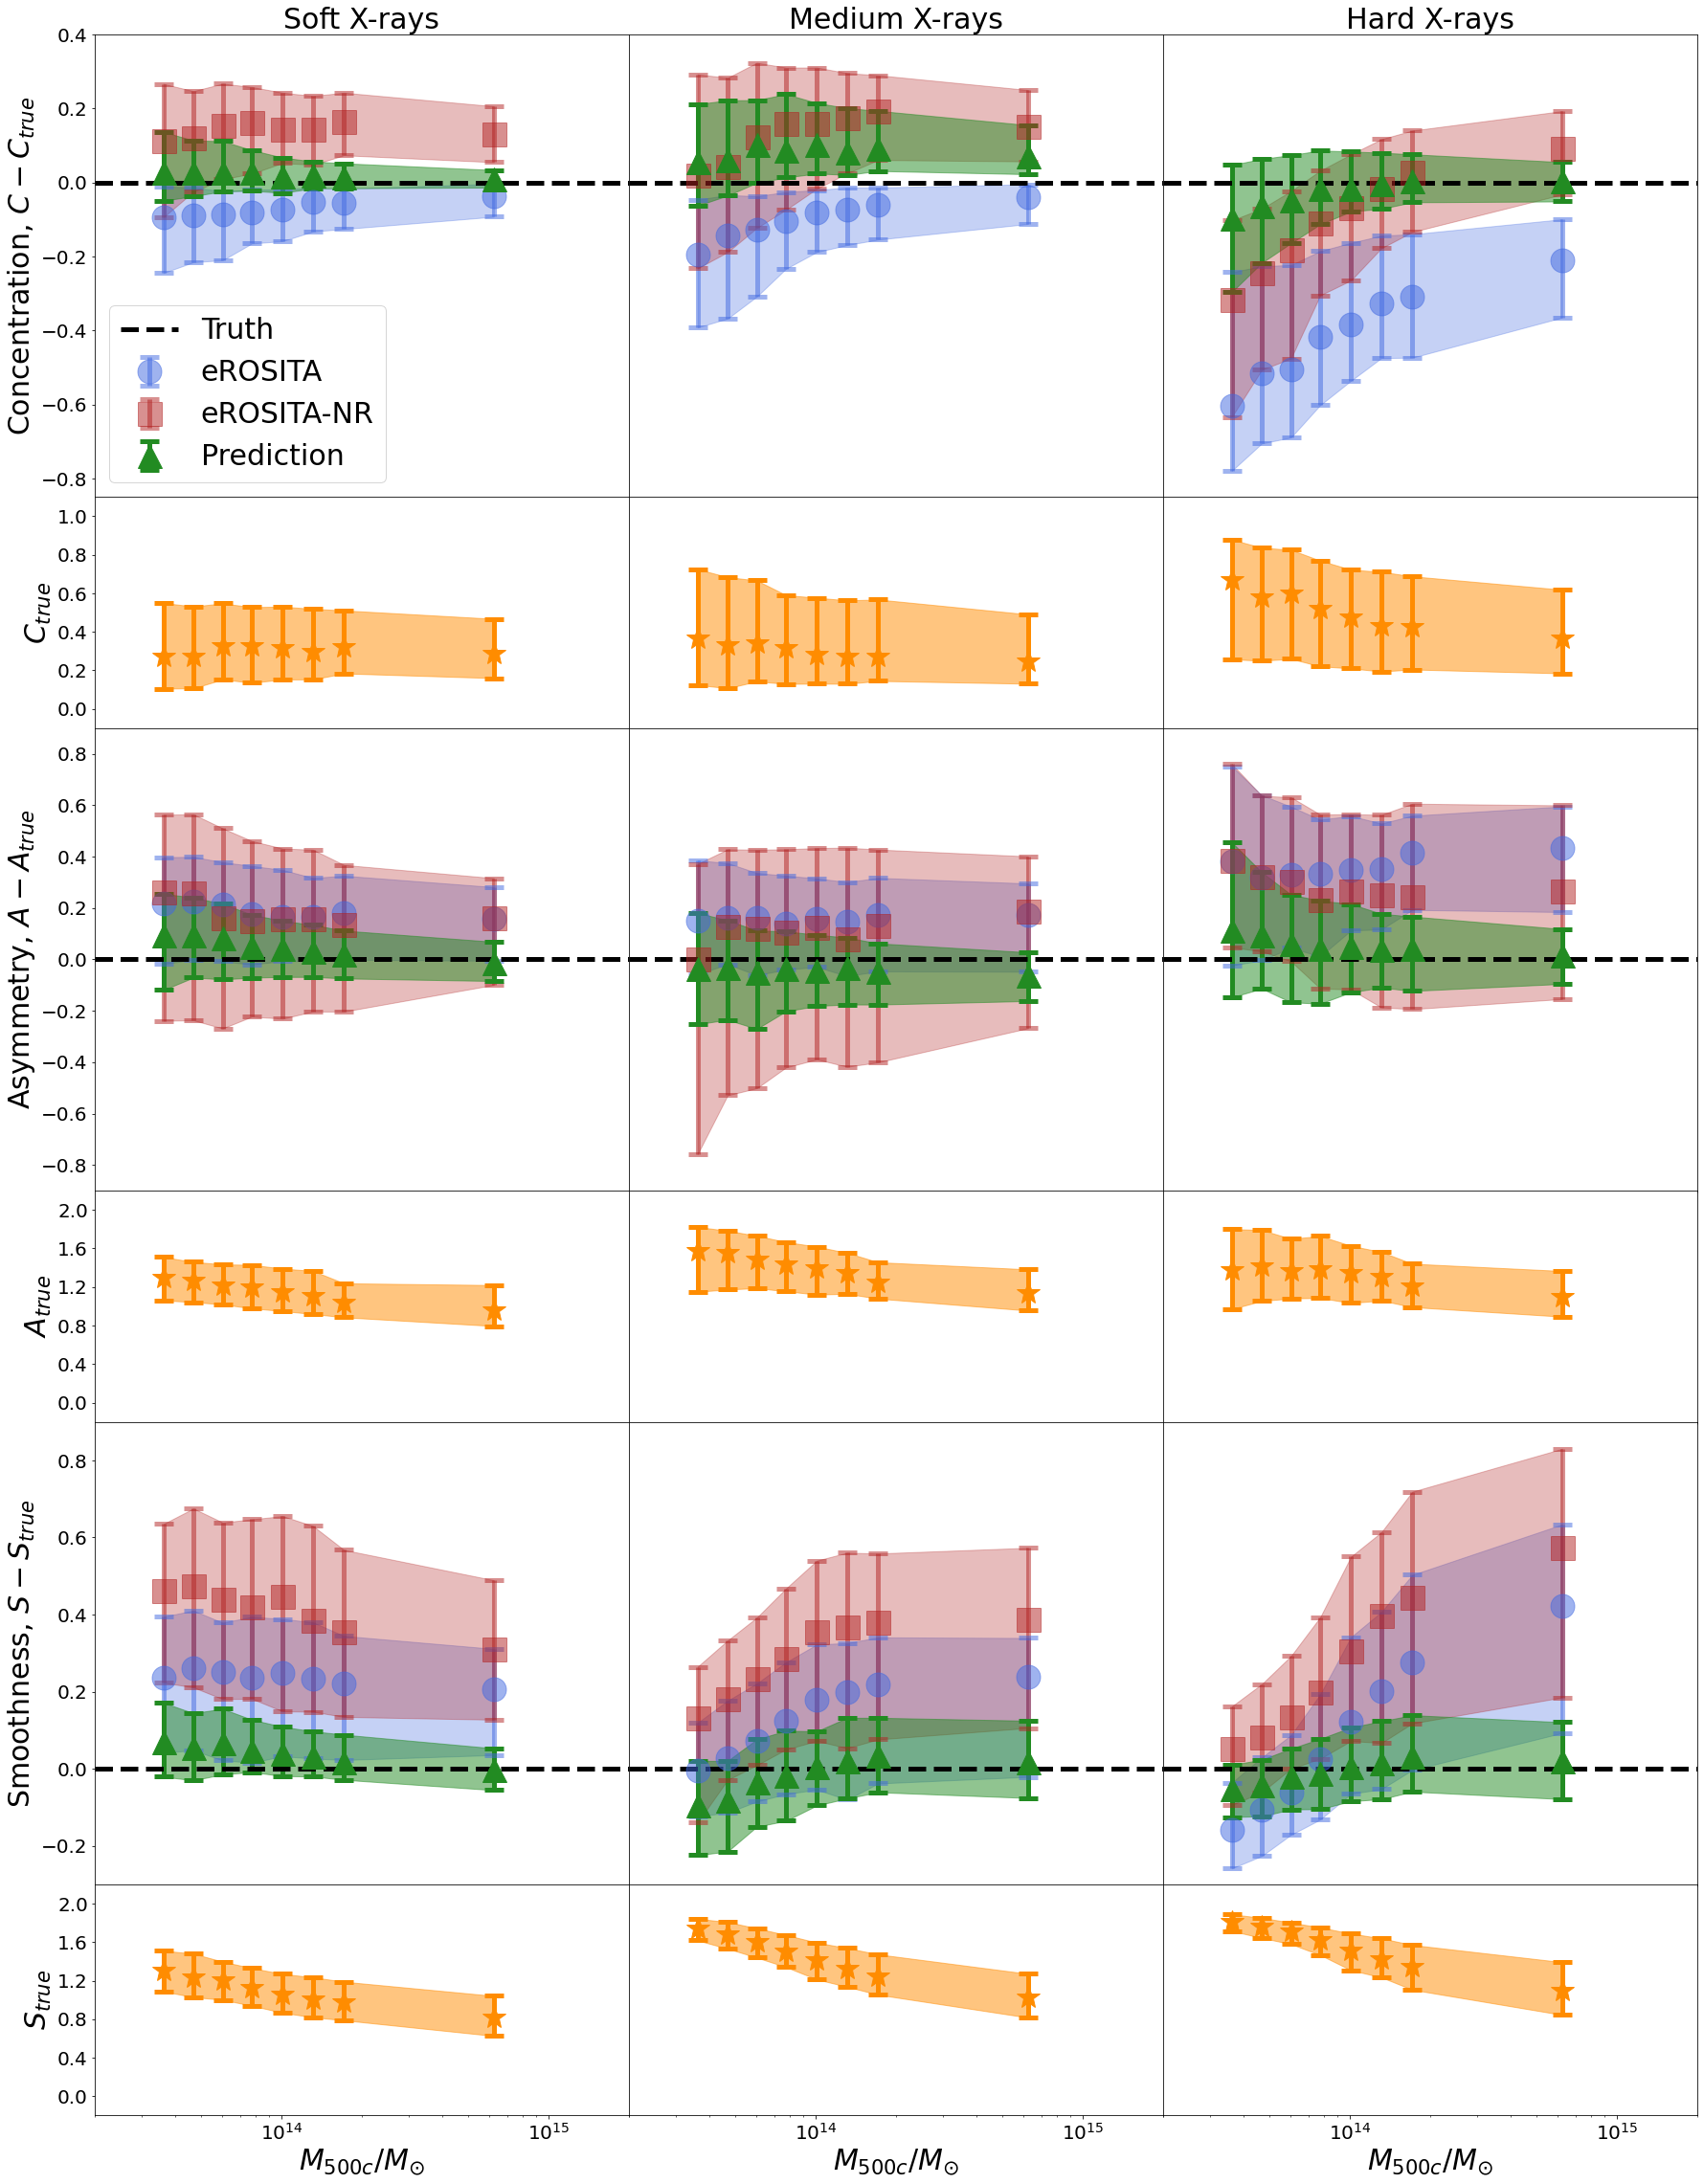
\includegraphics[width=\textwidth]{Ch2_Super_Obs/Mass_Dependence_072722.png}
\end{figure*}

\begin{figure*}
    \centering
    \caption{\raggedright Morphology parameter results are shown above. Morphology parameters, as derived from mock-\textit{eROSITA}, \textit{eROSITA}-NR (background subtracted), and prediction observations are compared to the true values, derived from the super observations. The top multicolored plots show the difference between observed parameter and true parameter, binned by mass. The bins are roughly equal in population. The points and error bars show the median and 16th to 84th percentile range of the results and are plotted in the middle of the mass bin range. The bottom orange plots illustrate the true parameter as a function of mass. The prediction derived constraints, shown in green, with the median values marked by triangles, are clearly superior to the alternatives. This is especially apparent in the soft band, where the median difference and scatter are small for all parameters. These results suggest our model produces morphologically accurate and precise observations without a noticeable mass bias for clusters between $\sim 10^{13}$ to $10^{15} M_{\odot}$.}
    \label{fig:mass_dep}
\end{figure*}

\section{Discussion}\label{ch2_discussion}
Our model demonstrates the powerful potential of machine learning in assessing the merit of follow-up observations. We have shown that our prediction images preserve morphology, which correlates to important galaxy cluster properties like dynamical state and core type. This is important, because to resolve outstanding questions about these properties we need high resolution, long duration, observations from instruments like \textit{Chandra}, which have limited availability. The model's useful prediction observations will allow galaxy cluster observers to effectively and efficiently evaluate which \textit{eROSITA}-observed clusters merit follow-up observation. Predicted observations are not a replacement for follow-up observations, nor are predicted morphology parameters a replacement for real morphology parameter measurements, but predictions are useful for determining if an \textit{eROSITA}-observed cluster is likely to have a property of interest (e.g., a cool core) that merits a follow-up observation. Machine learning models are most effective when used in an ethical way, with an understanding of their strengths and limitations. There are ways in which an informed user might adapt or improve an model. Below, we discuss the strengths and limitations of our model and the ways in which one might overcome those limitations.

\subsection{Classification}\label{classification}
A strength of our model, as we have shown, is that our prediction observations are more morphologically accurate than either \textit{eROSITA} or \textit{eROSITA}-NR observations. It is worth noting, however, that this relative accuracy can be applied in a variety of unexpected ways. For example, imagine an observer wishes to perform follow-up observations on only the most highly disturbed clusters. To do so, they would like to determine which clusters are in the 90th percentile of asymmetry. We can test this premise on our own data, by examining whether the 10\% most asymmetric clusters according to the prediction observations match the 10\% most asymmetric clusters as determined by the super observations. In doing so, we find that our trained model can determine whether a cluster is among the 10\% most asymmetric clusters with a true positive rate of 59\% and a false positive rate of 5\%. In other words, 59\% of clusters in the 90th percentile of true asymmetries are found in the 90th percentile of predicted asymmetries. Of clusters that are not in the 90th percentile of true asymmetries, only 5\% are found in the 90th percentile of predicted asymmetries. For identifying the 90th percentile of soft band concentration or soft band smoothness, the true positive (TPR) and false positive (FPR) rates improve to $\rm{TPR}_{C} = 82\%$, $\rm{FPR}_{C} = 2\%$, $\rm{TPR}_{S} = 73\%$, and $\rm{FPR}_{S} = 3\%$. The number of possible classifications is infinite and we cannot provide an exhaustive list of the true positive and false positive rates, but we encourage users to recognize this potential application of our model.

\subsection{Domain Shift}\label{Domain Shift}
A drawback of using simulated data is a problem known as domain or distributional shift \cite[see section 7 of ][for a discussion]{Amodei_2016}. Simulated data will invariably differ from real data. These differences, rooted in both the computational constraints of simulating a universe and in our still limited understanding of important cosmological and astrophysical phenomena, will limit the utility of a model trained solely on simulated data. The morphology parameters, by their nature, are deeply intertwined with the baryonic physics of galaxy clusters \cite[e.g.,][]{Lau_2011, Lau_2012, Chen_2019, Fernando_2021}. These physics are the most difficult to simulate, and the least well understood to model, and therefore often vary from cosmological simulation to cosmological simulation. This increases the likelihood that biases induced by domain shift will be present when our model is applied to real data, or data from a different cosmological simulation. In addition to simulation related biases, we are limited by the morphological parameter space of our data set. Clusters at the extremes of the parameter space, e.g., very smooth clusters, are relatively unrepresented. In the regions of cluster morphology parameter space with limited training data (see the bottom plots of Figures \ref{fig:concentration}, \ref{fig:asymmetry}, and \ref{fig:smoothness}) one should use caution with the assessment tool's predictions. 

A potential solution to this problem is to make use of what is known as transfer learning. We can retrain a model, previously trained on simulated observations, on pairs of observations (e.g., \textit{eROSITA} and \textit{Chandra} observations of the same clusters). This technique can correct the distributional shift between different data sets, in this case simulated and real data. It has the additional advantage of requiring many fewer real data observation pairs than would be required to train a new model completely on real data. This technique has been applied to a variety of problems in astronomy \cite[e.g.,][]{Ackermann_2018, Dominguez_2019, Perez_Carrasco_2019}.

\subsection{Redshift, Observing Time, and Resolution Dependence}\label{biases}
We are not the first to recognize the importance of morphology in sample selection.  For example, \cite{Mantz_2015} developed the symmetry–peakiness–alignment morphology specifically to provide a more robust characterization of cool core clusters across different redshifts and observing instruments. While we opt for an alternative construction of morphology for computational reasons, our concentration-asymmetry-smoothness morphology provides similar information about cool cores, and we characterize robustness issues related to observing instrument and redshift. In the case of redshift, we find no substantial redshift bias in concentration, asymmetry, or smoothness. This is true across all energy bands, but especially in the soft band. We also performed a minor analysis of the effects of different observing instruments ourselves, investigating the change in morphology parameter value for an individual cluster as a function of resolution and observing time (see Figure \ref{fig:morphology_variance}). We find parameter values do change as a function of observing time and resolution. However, our results also suggest that the uncertainty of morphology parameters is minimal, even for lower observing times and coarser resolutions. This suggests that, given a representative sample of clusters observed by a single instrument, the morphology parameters of a cluster still provide useful information when compared to the distribution of morphology parameters of clusters observed by that instrument. Given the number of clusters \textit{eROSITA} is expected to observe, this constraint is not problematic. Moreover, while morphology parameters derived from the observations of one instrument do not directly map to those derived from the observations of another, the relationship between morphology and observing instrument can be characterized. 

Our own model is proof that a machine learning model can learn the relationship between the morphology parameters of a 2 ks and 10 ks observation. This suggests that machine learning models could characterize the relationship between morphology parameters derived from the observations of one instrument to those derived from the observations of another. With that in mind, we advise that this or any other follow-up merit assessment tool be developed with careful consideration for its intended use. One use case we envision for our tool is informing observers as to whether a \textit{eROSITA}-observed cluster has an extreme morphology relative to other \textit{eROSITA}-observed clusters (e.g., very asymmetric vs very symmetric). This information would be useful in determining whether a cluster has a dynamical state or core type that merits selection for follow-up. On the other hand, if one intends to predict \textit{Chandra}-resolution morphology parameters exactly, then one should train using \textit{Chandra}-resolution images as the truth images instead of \textit{eROSITA}-resolution images like we did.

\begin{figure*}%[b]
    \centering
    %\null \vspace{-20pt}
    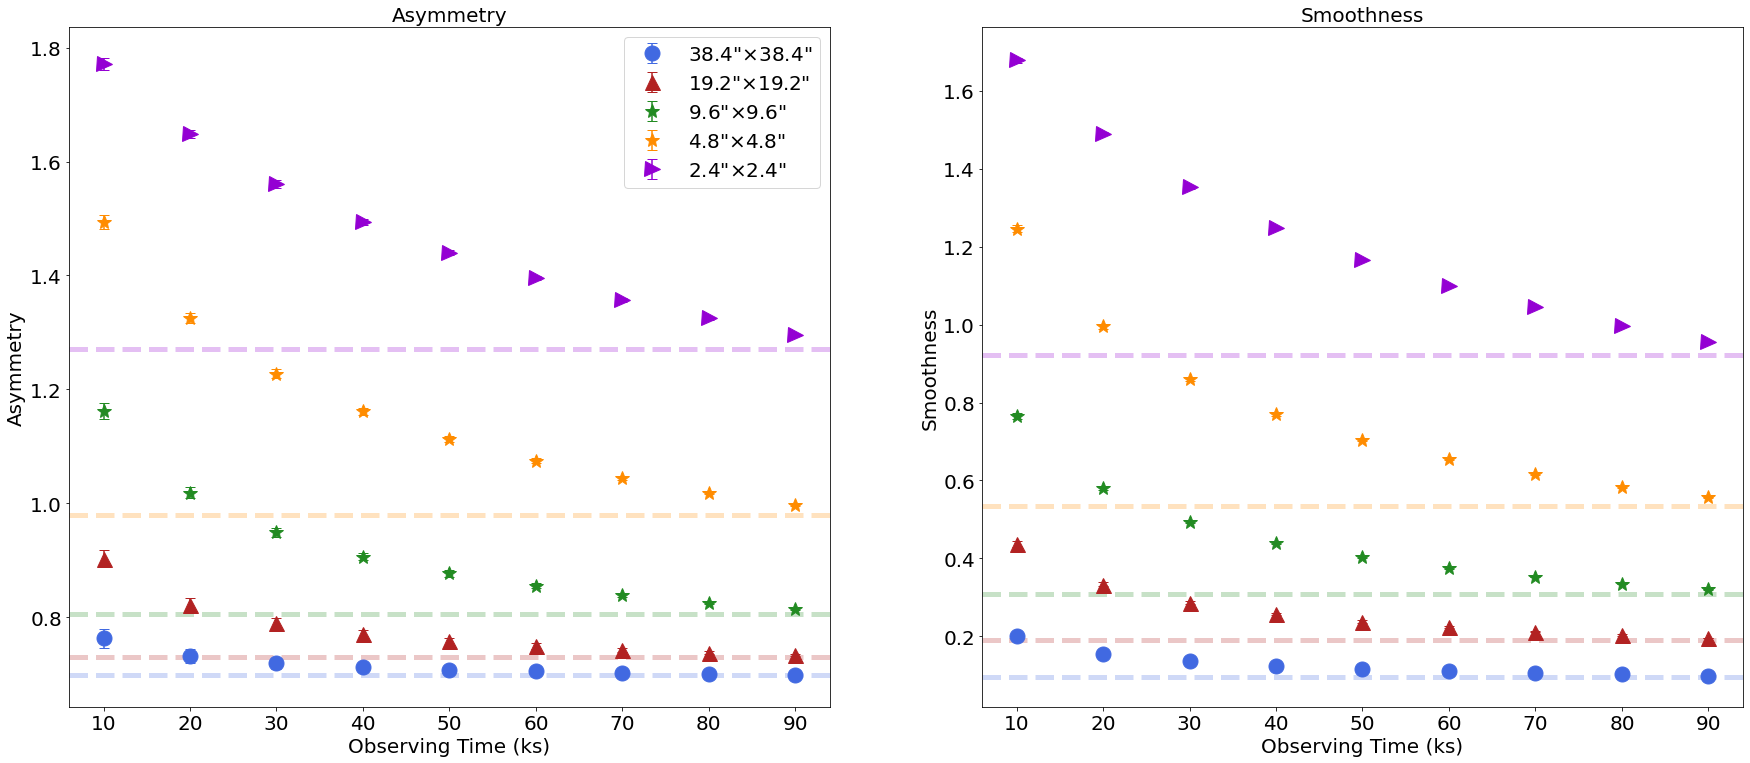
\includegraphics[width=\textwidth]{Ch2_Super_Obs/cluster2_Morphology_vs_N_photon_res_var_pix_size_072622.png}
    \caption{\raggedright Shown above are plots of the observed asymmetry and smoothness of a single cluster as a function of observing time and resolution. A single 100,000 second background-free mock observation of a $M_{500c}=1.48\times10^{14}M_{\odot}h^{-1}$ cluster at redshift $z=0.07$ with \textit{eROSITA} field of view was taken from \texttt{Magneticum} using \texttt{PHOX} \cite{magneticum,PHOX1,PHOX2}. Observing times were simulated by sampling different sized fractions of the photon list. The different colored and shaped points illustrate different pixel resolutions, denoted by the pixel size in arcseconds. The images we used for training our model, like \textit{eROSITA}, have a pixel size of 9.6"$\times$9.6". Error bars, representing the scatter of 1000 bootstrap samples, are also shown, but, in most cases, are smaller than the points. The dashed lines illustrate the parameter values for the full 100 ks observation. This plot illustrates that morphology parameters change depending on observing time and resolution, but also suggests that intrinsic uncertainty of morphology parameters on a 10 ks observation are small, albeit dependent on the intrinsic brightness of the source. Concentration is not shown, as its variation as a function of resolution and observing time is negligible.}
    \label{fig:morphology_variance}
\end{figure*}

\subsection{Alternative Metrics and Models}\label{Alternatives}

In our work, we aimed to create predictions that build on established techniques in the field of cluster cosmology. For computational and scientific reasons we opted for the simple but well established concentration, asymmetry, and smoothness parameters. While there is strong evidence of these parameters' correlation with our properties of interest \cite[e.g.,][]{Rasia_2013, Parekh_2015, Lovisari_2017, Green_2019}, these are not the only morphology parameters used in cluster cosmology and the statistical properties of these parameters are not well understood. This is especially true of the asymmetry parameter, where there exists plentiful literature on anisotropy tests and measures with better characterized statistical properties \cite[for examples and reviews of this topic see][]{mardia2000directional, feigelson2012modern, pewsey2013circular, baddeley2015spatial, RAJALA2018141}. While an analysis of the correlation of alternate anisotropy parameters to cluster properties of interest is outside the scope of this work, we encourage others to explore employing new measures of anisotropy to galaxy cluster cosmology.

Morphology is not the only potentially relevant observable for the outstanding questions in galaxy cluster cosmology. Other relevant properties such as X-ray scaling relations (e.g., Lx-Tx, Lx-M, Tx-M), X-ray surface brightness profiles, reconstruction of 3D gas and temperature profiles, or hydrostatic mass profiles might be of interest to X-ray observers. We chose morphology parameters because they are computationally easy to calculate (which is very relevant for training a model), applicable to observations of individual clusters, and are valid for the available simulation data. There is a wide parameter space of valid galaxy cluster properties to investigate, and moreover, our research is of potential interest to astronomy outside of X-ray galaxy cluster observation. We encourage others to explore this ample parameter space, but we opt to more fully explore what we view as the most promising avenue for success.

We chose to focus on the morphological accuracy of observations, and therefore designed our model appropriately for that purpose. Alternative algorithm architectures are also possible and ought to be considered depending on the priorities of the user. We considered different loss functions, including a perceptual loss function, inspired by \cite{ploss}, that uses the output of third layer of the VGG19 network \cite{VGG19}. An example prediction from that model is shown in Figure \ref{fig:loss_functions}. The perceptual loss function model produced prediction observations that better preserved concentration in the soft band than the morphology loss model. Moreover, the prediction images from the perceptual loss model are arguably more realistic, appearing smoother and less noisy, while clearly preserving substructure and AGN. However, the prediction observations did not preserve asymmetry or smoothness effectively, or preserve concentration in the hard band. We valued the preservation of asymmetry and smoothness by the morphology loss model higher than the improvement in concentration and appearance that the perceptual loss model offered, but we recognize that other observers might have different priorities. In addition, we considered using a standard UNET architecture \cite{UNET}, however it did not function well with our chosen loss function. The choice of evaluation metric, used to test the utility of the trained model, is also important. We chose to focus on morphology parameters, but many image-to-image machine learning models were designed instead to produce realistic-looking images that could fool human observers \cite[see][for examples of different image accuracy metrics, including human evaluation]{Dahl_2017}. Machine learning offers a wide parameter space in terms of algorithm hyperparameters and we do not argue that the model we have presented is the most optimal. Instead, we argue it illustrates that a machine learning approach to follow-up merit assessment is not only possible, but potentially more powerful than alternative solutions.

\begin{figure*}%[b]
    \centering
    %\null \vspace{-20pt}
    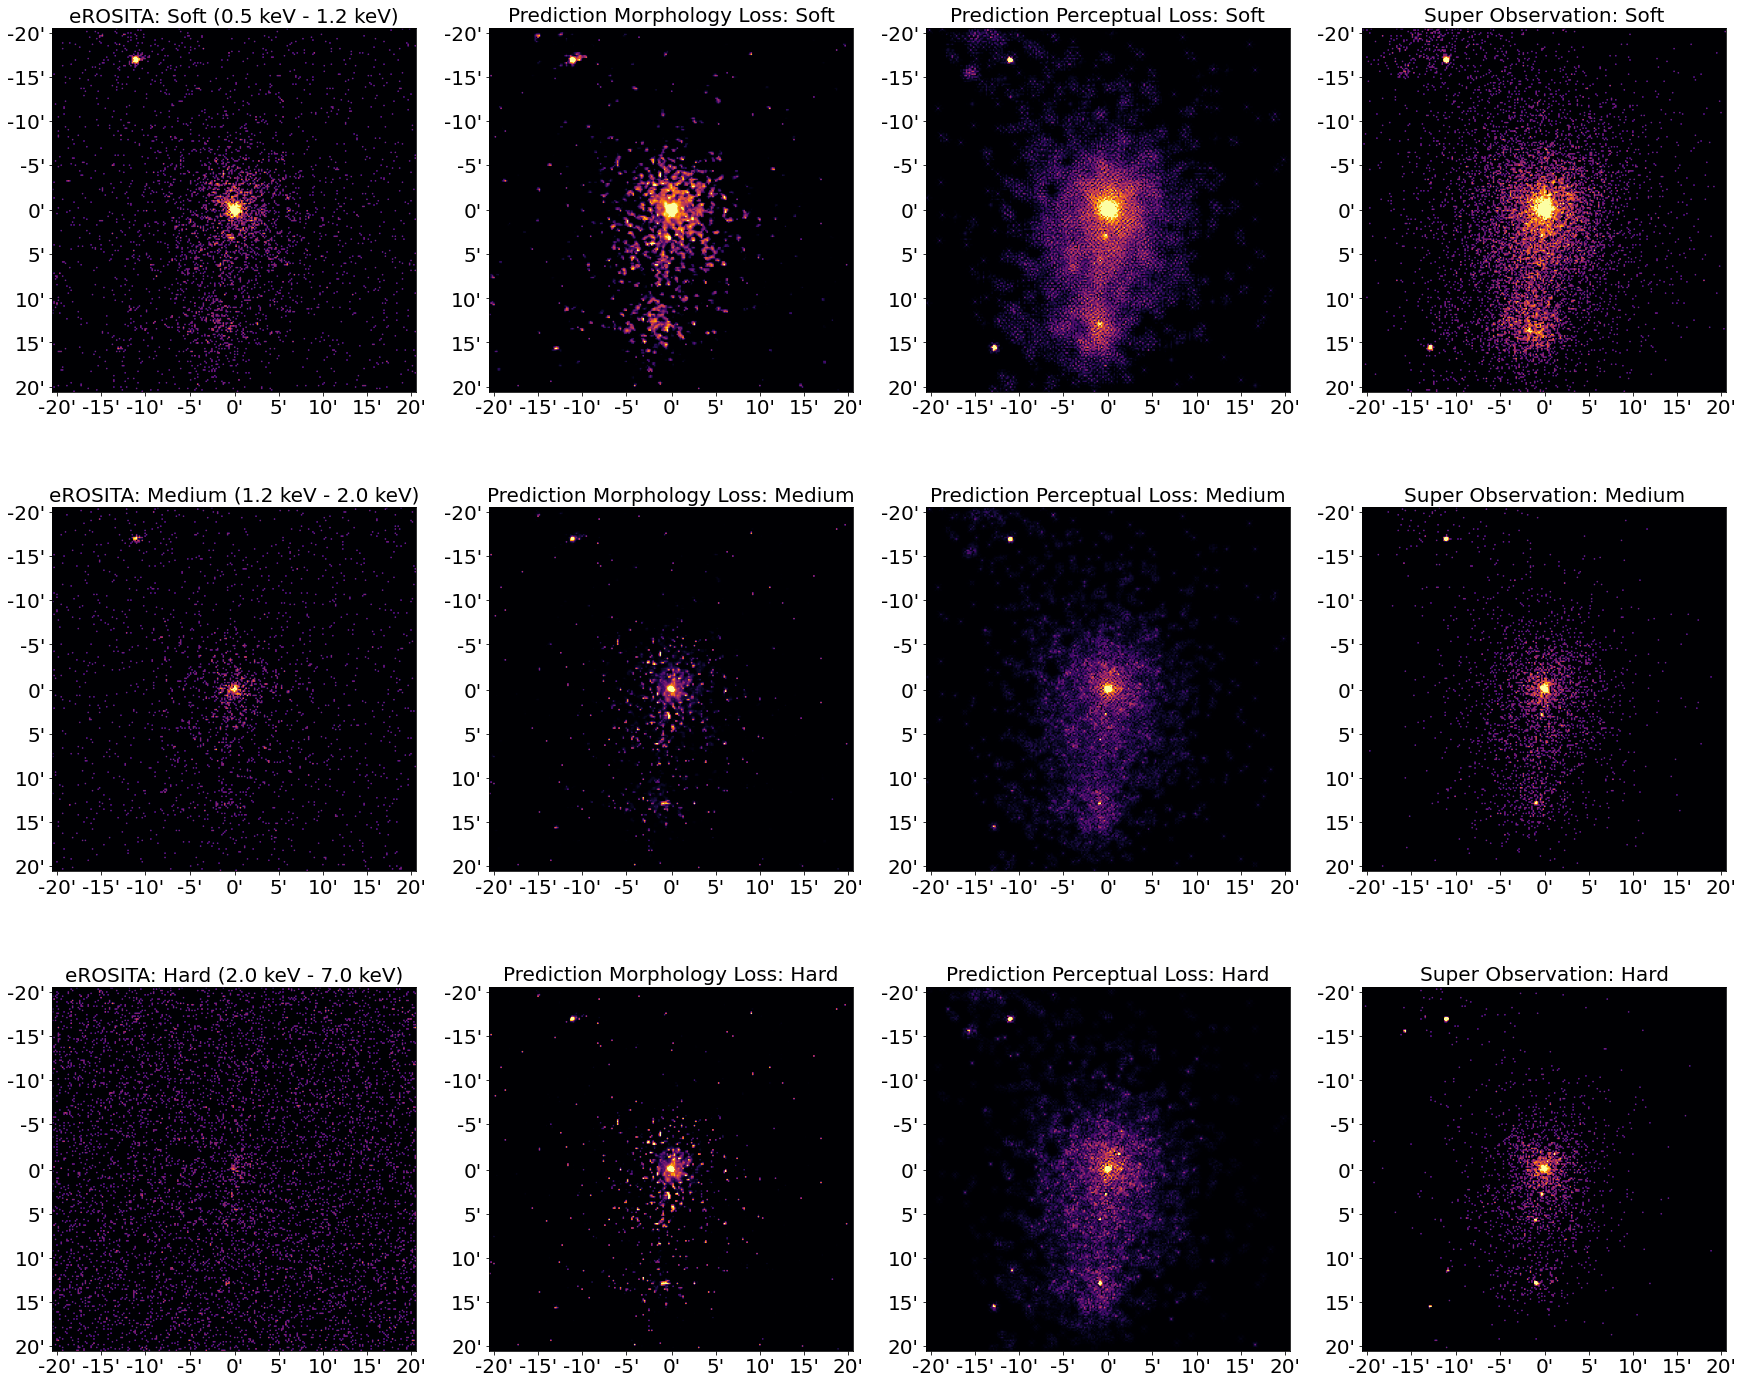
\includegraphics[width=\textwidth]{Ch2_Super_Obs/prediction_comparison_algorithm_070122_index_1850.png}
    \caption{\raggedright Plots of different observations of the same cluster. From left to right: mock eROSITA inputs, morphology loss predictions, perceptual loss predictions, and the super observation targets. The perceptual loss images performed worse at matching the morphology parameters of the super observations, so we instead presented on our morphology loss model. The perceptual loss model produces more visually appealing, and arguably realistic looking, predictions than the morphology loss model, however. The perceptual loss model also offered superior accuracy in the soft band concentration parameter. The perceptual loss model introduces non-physical structures into the image and its predictions have less accurate asymmetry and smoothness relative to the morphology loss model. We note this to emphasize the important decisions one must make in designing, training, and evaluating an algorithm. Our model was designed with a specific use case in mind, but other follow-up merit assessment algorithms might choose different algorithm architecture or accuracy metrics.}
    \label{fig:loss_functions}
\end{figure*}

\section{Conclusion}\label{ch2_conclusion}
Galaxy clusters are an important probe of cosmology and useful laboratories for understanding physics. Key cluster properties, like core cooling and dynamical state, remain poorly understood and are in need of further study. Detailed follow up observations provide insight to these properties, but resources for follow-up are limited and an efficient method for evaluating the merit of these observations is needed. Machine learning offers one such method.

Our follow-up merit assessment tool can predict background-free, long duration, observations with accurate and precise morphology parameters. Given morphology’s correlation with the aforementioned cluster properties \textemdash{} which are both important in there own right and useful for selecting clusters for dark matter studies and mass estimation \textemdash{} morphologically accurate observations will aid follow-up selection. Our model will therefore advance our understanding of galaxy cluster internal physics, galaxy cluster cosmology, and cosmology more broadly.

Additionally, our work illustrates how follow-up merit assessment might be approached for a variety of different observational goals. Our model was designed to prioritize morphological accuracy, however the model could be trained as needed to address different properties. In working on this problem we explored a wide range of models, many with their own strengths and deficiencies. We advocate that observers strongly consider the priorities of their own observations when designing a follow-up merit assessment tool and tailor it to their specific needs. When utilized appropriately, machine learning can be an incredibly powerful tool for advancing galaxy cluster cosmology.



\chapter{Self-Similar Mass Accretion History in Scale-Free Simulations} \label{chap:chap-3}


%%%% MUST: if the chapter is a reprint or submitted paper, you must declare it
%% you can use enumerate or itemize environment if you have more than one paper 
%% \mybibexclude{} will exclude this citation from the final bibliography
%% if this paper appears somewhere else then remove \mybibexclude{} command

\begin{singlespace}         % you can also use `onehalfspace` to relax the spacing
    This chapter is adapted from the following publication:
    
    \fullcite{Soltis_2024}. 
    %\mybibexclude{sol}
\end{singlespace} 

\section{Introduction}\label{ch3_introduction}
In our own Universe, the mass accretion history of halos plays an important role in the dynamical state of galaxy clusters \cite[for reviews, see][]{Molnar_2016, Pratt_2019}. These massive virialized objects can provide a useful probe of cosmology, however their dynamical state can bias cosmological parameter estimation \cite[e.g.,][]{Lau_2009, Nelson_2014, Shi_2015, Gianfagna_2021}. Similarly, galaxy clusters are a useful laboratory for studying dark matter \cite[e.g.,][]{Eckert_2022}. Here dynamical state, and thus mass accretion history, sometimes provides a more salutary role than with cosmological parameter constraints. In some cases, most famously the Bullet Cluster \cite{Clowe_2006}, an extreme dynamical state allows us to separately observe the dark matter and gas components. Mass accretion history is also thought to play an important role in the evolution of galaxies in clusters, with infalling galaxies losing gas to the surrounding intracluster medium \cite[for a review, see][]{Boselli_2022}.

Given the importance of halo mass accretion history in understanding cosmology, dark matter, and astrophysics, it is no surprise that there has been a great deal of interest in better understanding mass accretion history itself. Links have been found between mass accretion and a number of other important cluster properties, like concentration, asymmetry, the position of the brightest core galaxy relative to the X-ray centroid, and the splashback radius \cite[e.g.,][]{Lovisari_2017, Dupourque_2022, Shin_2023}. Efforts have been made to construct mass accretion or dynamical state proxies out of the observable morphology of galaxy clusters, or to estimate it more directly \cite{De_Luca_2021, Capalbo_2022, Perez_2023, Pizzardo_2023, Arendt_2024, Soltis_2025}. Research into the relationship between mass accretion history and cosmological parameters is also ongoing \cite[Warburton et al. in prep.;][]{Amoura_2024}.

To draw a link between mass accretion histories and observable properties of clusters, or to choices of cosmology, one typically needs to use cosmological simulations \cite[see][for a near exception, although $N$-body simulations were still used to inform and validate the method]{Pizzardo_2022}. Applying conclusions drawn from simulations faces an important challenge, however. What if the simulation is not physically accurate? How can we guarantee that the distribution of mass accretion histories in a simulation is representative of our Universe if we are unable to directly observe mass accretion history in our Universe? In this paper, we take an important step towards answering this question. 

Previous work has also sought to answer this question. For example, \cite{Mansfield_2021} examined the convergence of mass accretion rates in halos between lower and higher resolution dark matter only simulations. While this form of test is essential, we opt for a different, but complimentary, approach. We probe whether a simulation and halo finder deviate from expected behavior without relying on higher resolution simulations. This is important, because comparing to a higher resolution simulation can, at most, provide a relative test of convergence. However, higher resolution simulations are not guaranteed to be more converged to physically realistic results than lower resolution simulations.

Scale-free cosmologies present an ideal testing ground for evaluating mass accretion histories. In a scale-free cosmology, we expect any dimensionless physical property to behave self-similarly (see Section \ref{scale_free} for more details). Where a property deviates from self-similarity, we can say that it is dependent on non-physical properties of the simulation, or halo-finder, and is therefore not physically accurate. This presents a useful, and more absolute, probe of the robustness of halo mass accretion histories than can be attained by comparing simulations of different resolutions. Applying the results of this testing to other simulations and cosmologies is another challenge. As will be discussed in sections \ref{Abacus} and \ref{LCDM}, one can use the choice of spectral index to apply the results to other cosmologies. Moreover, future exploration of different $N$-body codes and spectral indices could provide upper bounds on the range of reliability of mass accretion histories, or other properties, for different simulations and use cases. 

It is important to emphasize that this scale-free test probes the accuracy of simulations in only a negative sense. Deviations from self-similarity suggest that a simulation and/or halo finder is unreliable. The presence of self-similarity, however, does not guarantee that the examined properties are physically realistic. Constraints from this test thus serve as an upper bound on the robustness of simulations.

Several papers have been written on using the \textsc{Abacus} $N$-body code and scale-free simulations. In \cite{Joyce_2021}, the self-similarity of the two point correlation function of particles in a scale-free simulation generated using \textsc{Abacus} is tested. In using this test to quantify the resolution of the simulation, the authors find that the length scales on which they observed convergence to self-similarity propagated from larger to smaller scales. This is a result that we will also observe. \cite{Leroy_2021} applies the same technique to investigate the convergence to self-similarity of the halo mass function and the halo-halo correlation function. In doing so they compare the performance of two different halo finders, a friends-of-friends algorithm and \textsc{Rockstar} \cite{Rockstar}. They observe good convergence using \textsc{Rockstar} and very limited convergence using the friends-of-friends algorithm. \cite{Garrison_2021_softening} once again uses the two point correlation function of particles in a scale-free simulation generated using \textsc{Abacus}, this time to test the impact of the softening scheme used. In addition to observing that convergence to self-similarity improves at smaller scales at late times, the analysis also confirmed the fiducial choice of softening regime (recapped briefly in Section \ref{Abacus}). \cite{Garrison_2022_k_nearest} use a $k$-nearest neighbor probability distribution to assess convergence. In doing so they probe the density at different particle and density scales, finding that spheres containing only 32 particles will be converged at densities typical of halos. 

Our work most closely builds off the methods and analysis of a series of papers, \cite{Maleubre_2022}, \cite{Maleubre_2023}, and \cite{Maleubre_2024}. \cite{Maleubre_2022} analyzed the convergence of the matter power spectrum, while \cite{Maleubre_2023} examined the convergence of radial pair-wise velocity of particles. Finally, \cite{Maleubre_2024} extends on the previous works by investigating the convergence of the halo mass function, two point correlation function, and the mean radial pair-wise velocity of halos. Similar to \cite{Leroy_2021} and exactly as in this work, \cite{Maleubre_2024} compares the performance of two halo finders, \textsc{Rockstar} \cite{Rockstar} and \textsc{CompaSO} \cite{CompaSO}. The results of that work are in line with previous results, namely that \textsc{Rockstar} performs better than other halo finders, and that convergence improves as the simulation evolves. 

In this paper we use the self-similarity property of scale-free cosmologies to probe the robustness of halo mass accretion histories. We use a scale-free simulation from the same family of \textsc{Abacus} simulations \cite{Garrison_2021_ABACUS} used in previous work \cite[e.g,][]{Maleubre_2024}. Like \cite{Maleubre_2024}, we compare the performance of two halo finders, \textsc{Rockstar} \cite{Rockstar} and \textsc{CompaSO} \cite{CompaSO}. Our work serves as a natural extension of \cite{Maleubre_2024}, in so far as we use the same simulation, test the same halo finders, and that our analysis probes the convergence of the halo merger trees. In this work, we present bounds on self-similarity for both halo finders and the prospect for applying them to other simulations. 

This paper is structured as follows. In Section \ref{ch3_methods} we provide a brief overview of scale-free cosmologies (\ref{scale_free}), a description of our definition of mass accretion history (\ref{mah_def}), and explain our criteria for evaluating convergence to self-similarity (\ref{self_similarity}). In Section \ref{sims_and_finders} we discuss our choice of $N$-body code and simulation (\ref{Abacus}), and the two halo finders used (\ref{finders_descriptions}). Next, in Section \ref{ch3_results}, we describe our results for both halo finders (\ref{rockstar_results}, \ref{compaso_results}). Finally, we discuss the results in Section \ref{ch3_discussion} and conclude in Section \ref{ch3_conclusion}.

\section{Methodology}\label{ch3_methods}
\subsection{Scale-Free Cosmology}\label{scale_free}
$N$-body simulations with a scale-free cosmology have been used to study the behavior and robustness of halo properties, and the applicability of the stable clustering analytical approximation \cite[e.g.,][]{Efstathiou_1988, Colombi_1996, Cole_1996, Joyce_2007, Knollmann_2008, Elahi_2009}. Following the format of previous work \cite[][]{Joyce_2021, Leroy_2021, Garrison_2021_softening, Garrison_2022_k_nearest, Maleubre_2022, Maleubre_2023, Maleubre_2024}, we use the property of self-similarity in scale-free simulations to test the robustness of halo mass accretion histories. Below we briefly summarize scale-free simulations and self-similarity following the discussion in \cite{Maleubre_2024}. For further discussion of scale-free simulations and their properties, see \cite{Joyce_2021} and citations therein.

Scale-free cosmologies are Einstein-de Sitter universes, $\Omega_{\mathrm{Tot}} = \Omega_{M} = 1$, with a power law spectrum of initial fluctuations, $P(k) \propto k^{n}$, and a $a(t) \propto t^{2/3}$ expansion law. With these conditions, there exists only one relevant length scale, $R_{\mathrm{NL}}$, the scale at which the variance of the normalized linear amplitude of fluctuations, $\sigma_{\mathrm{lin}}$, is equal to one. This length scale is known as the scale of non-linearity, defined by
\begin{equation}\label{eqn:def_nonlinear_scale}
    \sigma_{\mathrm{lin}}(R_{\mathrm{NL}},a) = 1.
\end{equation}
From linear perturbation theory, we deduce that
\begin{equation}\label{eqn:nonlinear_evolution}
    R_{\mathrm{NL}} \propto a^{\frac{2}{3+n}}
\end{equation}
where $n$ is the spectral index. This suggests that, without the introduction of other length scales, the clustering must evolve self-similarly. Thus any dimensionless clustering statistic can be rescaled such that
\begin{equation}\label{eqn:rescaling}
    F(X,a) = F_0\left(\frac{X}{X_{\mathrm{NL}}(a)}\right).
\end{equation}
Here $X_{\mathrm{NL}}$ contains the time dependence of any quantity with the dimensions of $X$.

We can define $R_{\mathrm{NL}}$ in terms of the initial conditions of the simulation using equations \ref{eqn:def_nonlinear_scale} and \ref{eqn:nonlinear_evolution}. That is

\begin{equation}\label{eqn:R_def}
    R_{\mathrm{NL}}(a) = \ell \left(\frac{a}{a_i} \sigma_i \right)^{\frac{2}{3+n}}.
\end{equation}
Here $\sigma_i$ is variance of the normalized linear amplitude of fluctuations at $a_i$, where the initial particle spacing is set to $\ell$ (i.e., $\sigma_i \equiv \sigma_{\mathrm{lin}}(\ell, a_i)$). Using Equation \ref{eqn:R_def}, we can define a non-linear mass scale as
\begin{equation}\label{eqn:nonlinearmass}
    M_{\mathrm{NL}} = \frac{4 \pi}{3} \bar{\rho} R_{\mathrm{NL}}^3(a) = \frac{4 \pi}{3} M_{particle} \left(\sigma_i \frac{a}{a_i}\right)^{\frac{6}{3+n}}.
\end{equation}
We will use this non-linear mass scale to rescale our mass accretion history definition in the following subsections.

\subsection{Defining Halo Mass Accretion}\label{mah_def}

To take advantage of the self-similarity of dimensionless statistics in scale-free simulations, we must construct a dimensionless halo mass accretion history. Our definition is also constrained by the discrete temporal outputs of our simulation, so we define our mass accretion history in terms of the difference in the mass of halos and their descendants over two consecutive snapshots. Thus our mass accretion history can also be thought of as a mass accretion rate. With these constraints in mind, we define the halo mass accretion history of the $j$th cluster, $\Gamma_j$, as
\begin{equation} \label{eqn:mahofmofj}%\label{eqn:mahofm}
\Gamma_j(a) = \frac{d \log(M)}{d \log(a)}
\end{equation}
As discussed, we must approximate the derivative in Equation \ref{eqn:mahofmofj} using the discrete snapshot outputs of the simulation. Conveniently, these snapshots are evenly spaced in $\log(a)$ (see Section \ref{Abacus} and Equation \ref{eqn:log_a_spacing}), thus we find that for the $j$th cluster, the mean mass accretion history at time $i$ is proportional to
\begin{equation} \label{eqn:approx_mahofmofj}
   \Gamma_j(a_i) \propto \frac{M_j(a_{i+1}) - M_j(a_{i})}{M_j(a_{i})}
\end{equation}
Therefore, the mass accretion history of the $j$th cluster is the difference between the mass of the $j$th halo at snapshot $i$, $M_j\left(a_{i}\right)$, and the mass of its most massive descendant at the following snapshot, $M_j\left(a_{i+1}\right)$, all normalized by $M_j\left(a_{i}\right)$.

We are not interested in the mass accretion rate of individual clusters, however, but in the population level behavior. Therefore, we define a mean mass accretion history, $\Gamma$, over the population of clusters at time $i$ with mass $M$ as
\begin{equation} \label{eqn:mahofm}
   \Gamma(M, a_i) = \left<\Gamma_j(a_i)\right> \propto \left<\frac{M_j(a_{i+1}) - M_j(a_{i})}{M_j(a_{i})}\right>
\end{equation}
where the angle brackets represent the average over halos whose masses satisfy
\begin{equation} \label{eqn:av_over_mahofm}
 M_j \in \left(M, M + d M\right).
\end{equation}
Note that this mean mass accretion history is now a function of both halo mass and scale factor.

Following the principles discussed in Section \ref{scale_free}, we rescale Equation \ref{eqn:mahofm} according to Equation \ref{eqn:rescaling}. In this case, the rescaling unit is the mass scale of non-linearity, seen in Equation \ref{eqn:nonlinearmass}. The resulting mean halo mass accretion history definition is
\begin{equation} \label{eqn:mahofMNL}
\begin{split}
\Gamma\left(\frac{M}{M_{\mathrm{NL}}}\right) & \propto \left<\frac{M_j(a_{i+1}) - M_j(a_{i})}{M_j(a_{i})}\right> \\
 \frac{M_j}{M_{\mathrm{NL}(a_i)}} & \in \left(\frac{M}{M_{\mathrm{NL}}}, \frac{M}{M_{\mathrm{NL}}} + d \frac{M}{M_{\mathrm{NL}}}\right).
\end{split}
\end{equation}
The only change between Equation \ref{eqn:mahofm} and \ref{eqn:mahofMNL} is that the halos in the self-similar mass accretion history definition are now averaged by their rescaled mass, $M/M_{\mathrm{NL}}$. The result of this is that $\Gamma$ is now only a function of this rescaled mass bin. If our simulation is perfectly scale-free, and our halo finder is not introducing any non-physical scales, we should not expect to see any additional time dependence. In practice, we observe deviations from self-similarity, and therefore our observed mean mass accretion history does have an additional time dependence (i.e., $\Gamma_{\mathrm{obs}}(M/M_{NL}, a)$).

For our rescaled mass bins, we use 40 logarithmically spaced bins ranging $10^{-3}$ to $10^{2}$. This provides good coverage of the halo population, with sufficiently dense binning to explore interesting changes in behavior without sacrificing a sufficient population size per bin. The effect of rescaling is demonstrated in Figure \ref{fig:rescaling_example} and Figure \ref{fig:CompaSO_rescaling_example}. Self-similarity is observed as a consistency in values of $\Gamma$ over time, for a given rescaled mass bin.

\begin{figure*}
    \centering
    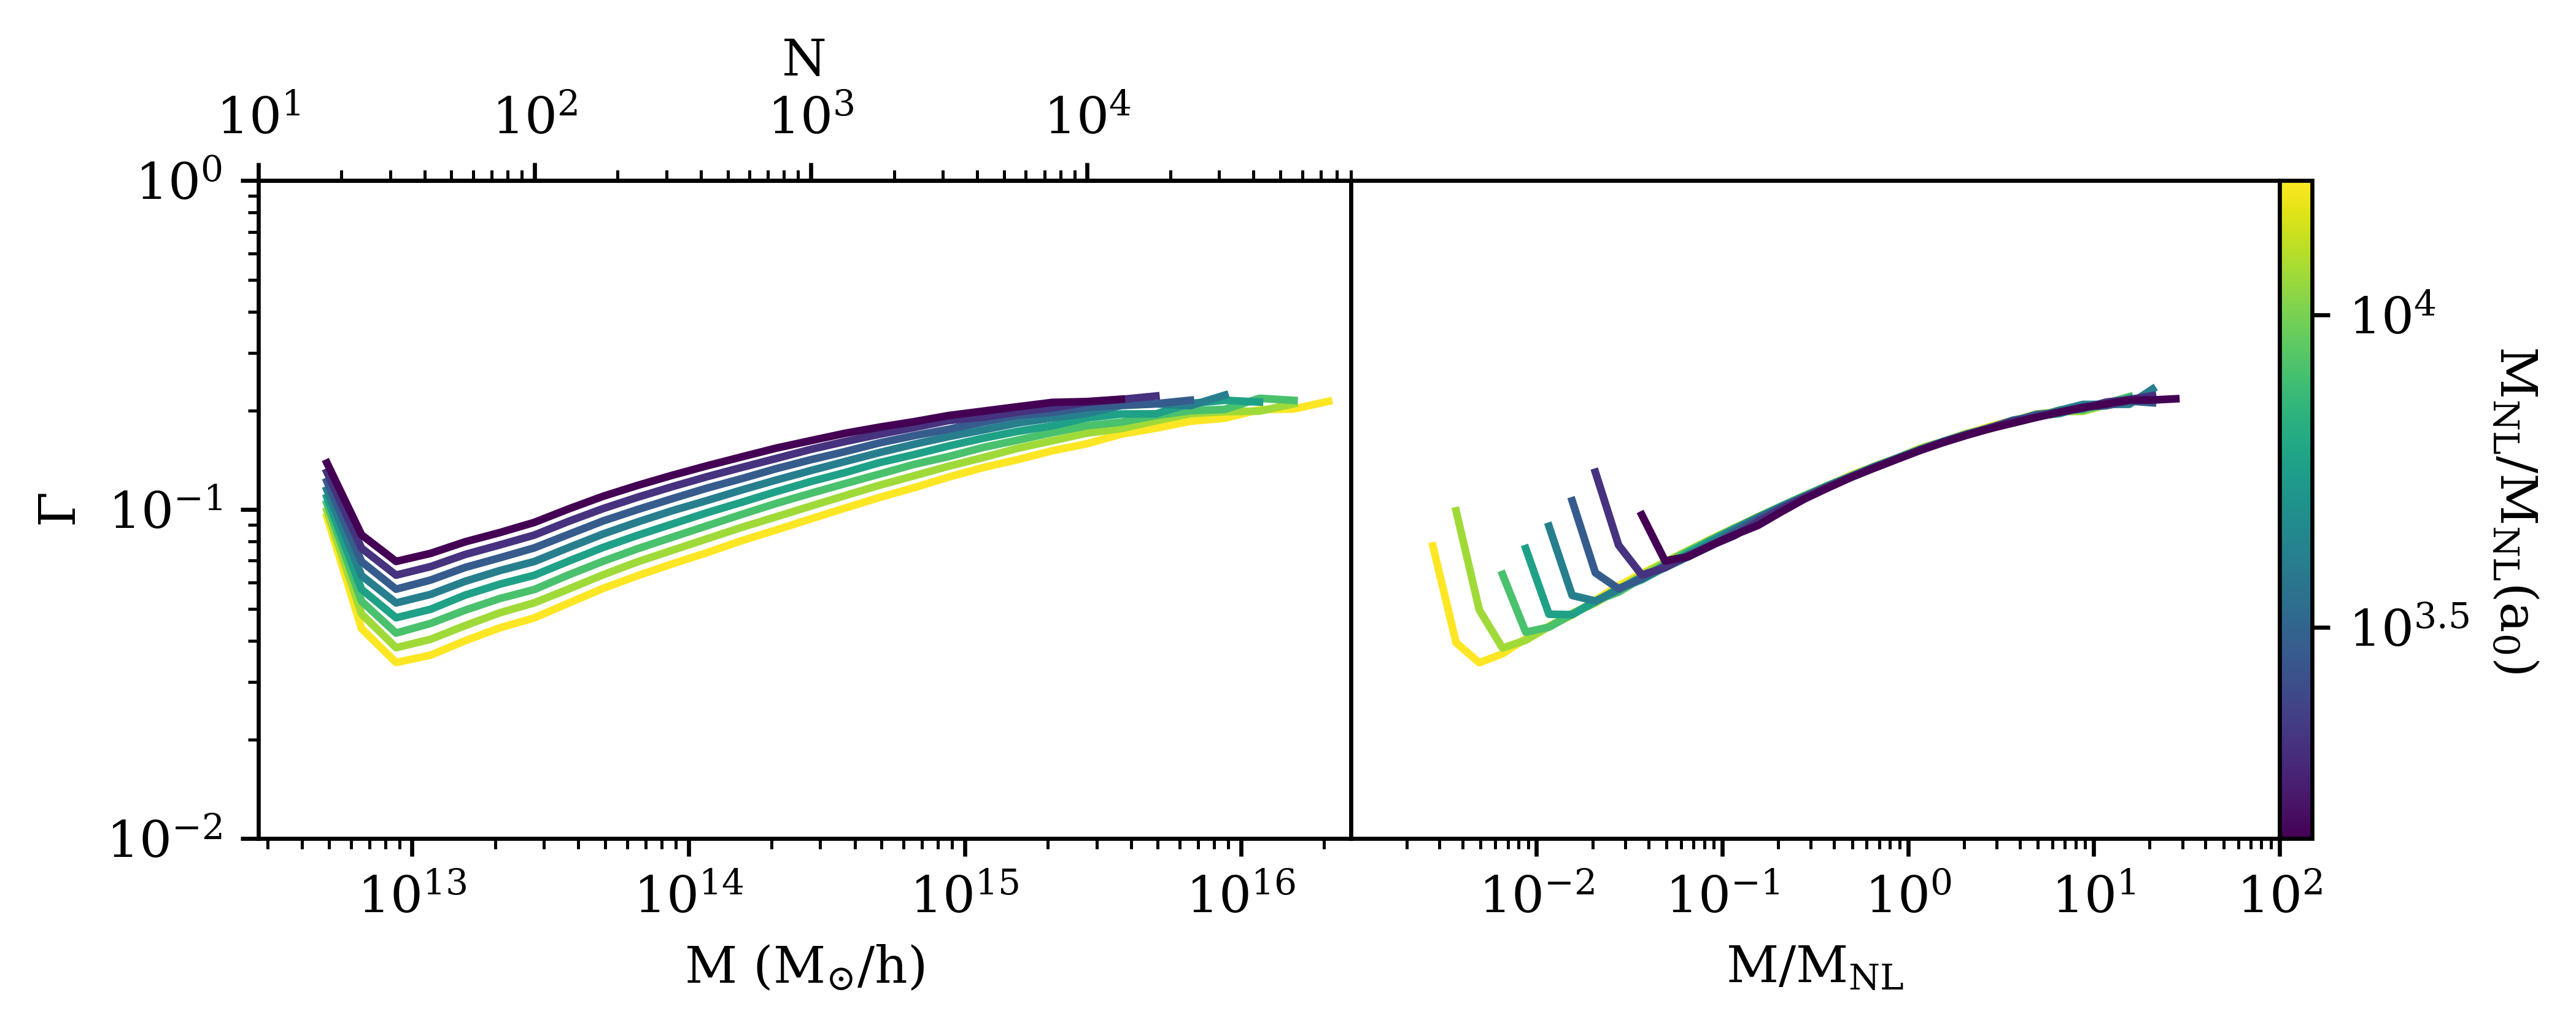
\includegraphics[width=\textwidth]{Ch3_Self_Sim/Paper_Plots_gtr20/ROCKSTAR_n15_z_mean_past_joyce_mah_M200c_gtr20_vs_M_and_M_M_NL.png}
    \caption{\raggedright The mass accretion history, $\Gamma$, for the last 8 snapshots of our simulation of a scale-free model with $n=-1.5$, found using the \textsc{Rockstar} halo finder. The plot on the left shows the mean mass accretion history ($\Gamma$) versus the halo mass ($M$) and the halo particle count ($N$), where the mass and particle count are defined by the center of the mass bin used. The plot on the right shows the self-similar rescaling of $\Gamma$, now plotted versus the rescaled mass, $M/M_{\mathrm{NL}}$. Note that the lines in the $\Gamma$ vs $M/M_{\mathrm{NL}}$ plot now fall on top of each other near $M/M_{\mathrm{NL}} \sim 1$, indicating that $\Gamma$ is self-similar in that region. The color illustrates the time step of the lines in terms of the multiplicative change in the non-linear mass since $a_0$. For more information on the snapshot time steps, see Section \ref{Abacus} and Equation \ref{eqn:log_a_spacing}.}
    \label{fig:rescaling_example}
\end{figure*}

\begin{figure*}
    \centering
    \includegraphics[width=\textwidth]{Ch3_Self_Sim/Paper_Plots_gtr20/CompaSO_n15_z_mean_past_joyce_mah_M200c_gtr20_vs_M_and_M_M_NL.png}
    \caption{\raggedright Above is a similar figure to Figure \ref{fig:rescaling_example}, but for mass accretion histories calculated using \textsc{CompaSO}. Note, that as pointed out in Section \ref{compaso_results}, the last two snapshots were not available for the \textsc{CompaSO} data, so the last snapshot available is $\log_2(a/a_0) = 3.25$ instead of $3.5$. The behavior illustrated in this plot is similar to Figure \ref{fig:rescaling_example}, with self-similarity apparent at $M/M_{\mathrm{NL}}\sim 1$. However, unlike Figure \ref{fig:rescaling_example}, the the results diverge from self-similarity at late times. The difficulty the \textsc{CompaSO} halo finder has with high mass halos is discussed in sections \ref{compaso_results} and \ref{comparing_finders}.} 
    \label{fig:CompaSO_rescaling_example}
\end{figure*}

\subsection{Evaluating Convergence to Self-Similarity}\label{self_similarity}
To evaluate the convergence of our chosen halo mass accretion metric to self-similarity we adopt the convention used in previous work \cite{Maleubre_2022,Maleubre_2023,Maleubre_2024}. In rescaled units, self-similarity is observed as the absence of temporal evolution. To quantitatively measure the convergence of halo mass accretion history to self-similarity, we then must evaluate the rescaled halo mass accretion history deviation from flatness, as a function of time (see Figure \ref{fig:Rockstar_CompaSO_mah_v_a}). Below, we provide an overview of our method.

\begin{figure*}
\centering
\begin{subfigure}{.49\textwidth}
\centering
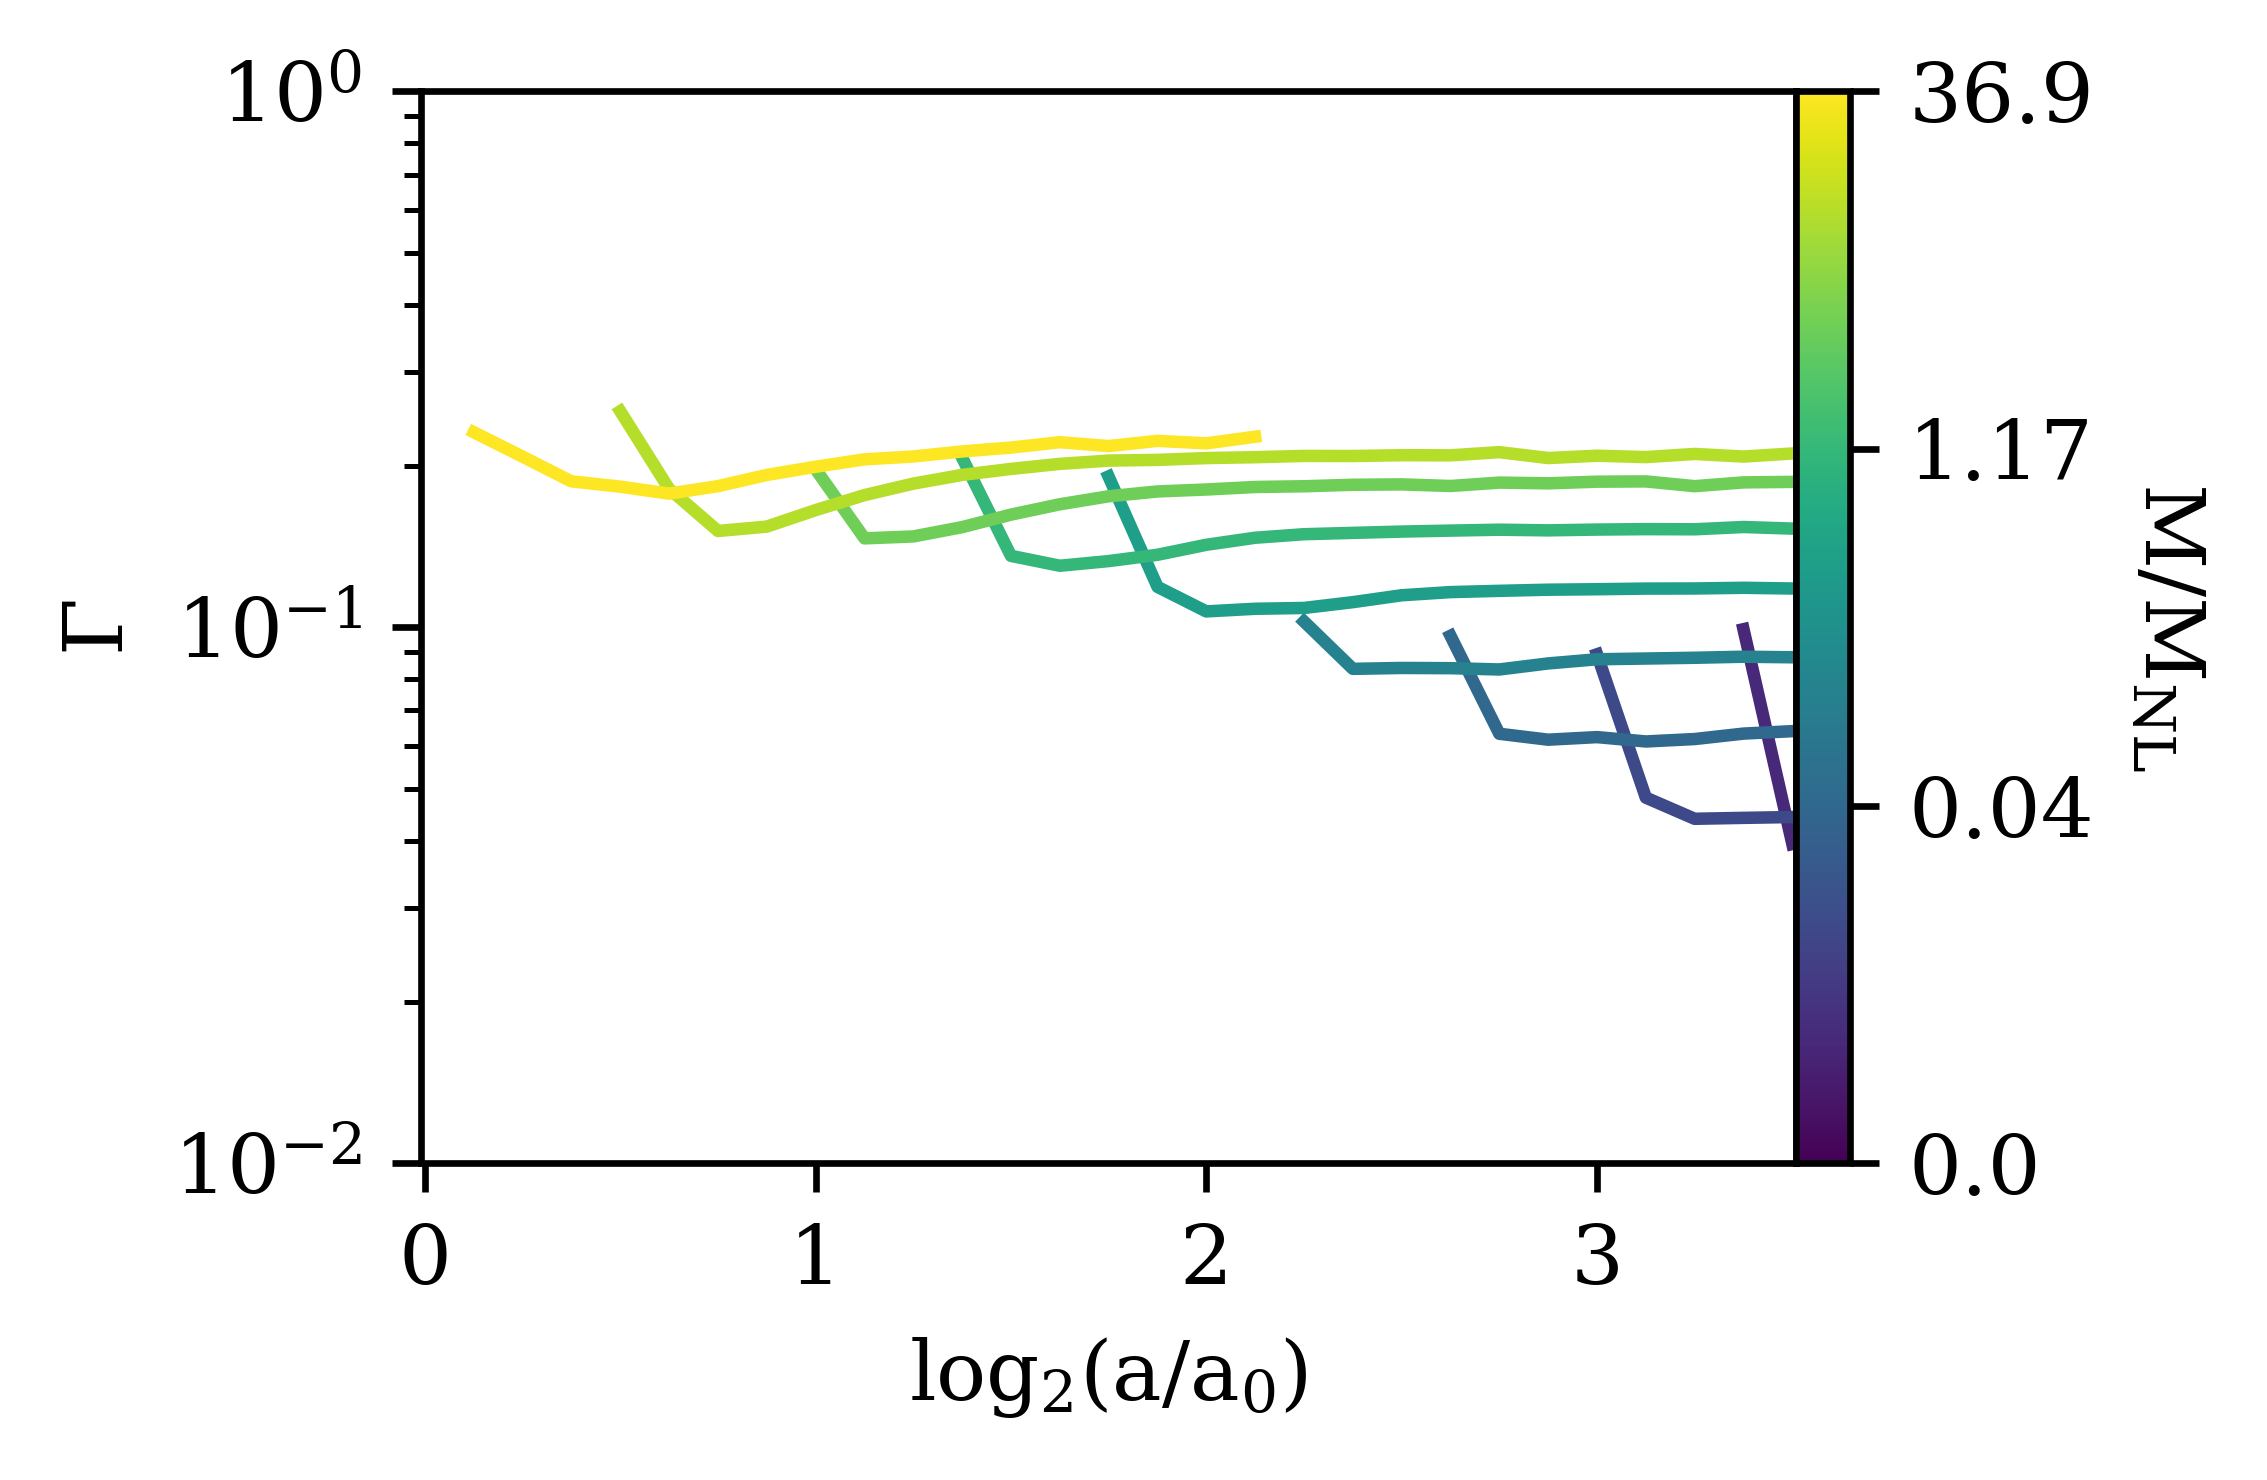
\includegraphics[width=\textwidth]{Ch3_Self_Sim/Paper_Plots_gtr20/ROCKSTAR_n15_z_mean_past_joyce_mah_M200c_gtr20_vs_a_continuous_spectrum.png}
\caption{\textsc{Rockstar}}
\end{subfigure}
\hfil
\begin{subfigure}{.49\textwidth}
\centering
\includegraphics[width=\textwidth]{Ch3_Self_Sim/Paper_Plots_gtr20/CompaSO_n15_z_mean_past_joyce_mah_M200c_gtr20_vs_a_continuous_spectrum.png}
\caption{\textsc{CompaSO}}
\end{subfigure}
\caption{\raggedright Above are the mass accretion histories ($\Gamma$) plotted against the doubling factor of the scale factor, $\log_2(a/a_0)$. Each line denotes the mass accretion history of a specific rescaled mass bin ($M/M_{\mathrm{NL}}$). In this presentation, the self-similarity discussed in section $\ref{ch3_methods}$ appears as a flattening of the $\Gamma$ vs $\log_2(a/a_0)$ line. As with Figures \ref{fig:rescaling_example} and \ref{fig:CompaSO_rescaling_example}, one can observe the very different late time behaviors of \textsc{Rockstar} (a) and \textsc{CompaSO} (b). While mass accretion histories tend towards flatness at late times for \textsc{Rockstar}, a clear drop in mass accretion history is visible for the highest rescaled mass bins for \textsc{CompaSO} results.}
\label{fig:Rockstar_CompaSO_mah_v_a}
\end{figure*}

First, we look for minimal variation over time in the mass accretion history, $\Gamma$, for each rescaled mass bin, $M/M_{\mathrm{NL}}$. Starting with the earliest times, we calculate $\Delta_1$ in regions of 5 consecutive snapshots as
\begin{equation}\label{eqn:delta1}
    \Delta_{1}\left(\frac{M}{M_{\mathrm{NL}}}, a_{i}, ..., a_{i+k}\right) = \left|\frac{\Gamma_{\mathrm{max}} - \Gamma_{\mathrm{min}}}{2\left<\Gamma\right>}\right|
\end{equation}
where the number of snapshots used, $k$ is equal to $5$ and $\Gamma_{\mathrm{max}}$ and $\Gamma_{\mathrm{min}}$ are calculated over the 5 snapshots (i.e., $a_{i}$ through $a_{i+k}$). We chose this window size conservatively to avoid spurious detection of self-similarity, while avoiding eliminating regions of substantial convergence. The general shape of the regions of convergence are robust to changes in window width, but the percent convergence of specific bins changes (see Section \ref{varying_bin_width}). If $\Delta_1 \leq X\%$, where $X\%$ is the desired level of convergence to self-similarity, we then move on to step two.

In the second step, we evaluate the convergence of each individual snapshot of $\Gamma$ for a given $M/M_{\mathrm{NL}}$ bin using $\Delta_2$ in Equation \ref{eqn:delta2}. Values are compared to the $\left<\Gamma\right>$ value of the window that passed step one. If more than one window passed step one, $\left<\Gamma\right>$ is equal to the average value of all the snapshots that passed in step one.\footnote{This is a modification of the method used in \cite{Maleubre_2024} and their earlier works, where they choose the window with the minimum $\Delta_1$ value. We find that taking the mean offers greater stability in measuring the convergence of $\Gamma$ than the previous method, however both methods yield broadly similar results.}
\begin{equation}\label{eqn:delta2}
    \Delta_2\left(\frac{M}{M_{\mathrm{NL}}}, a\right) = \left|\frac{\left<\Gamma\right> - \Gamma(\frac{M}{M_{\mathrm{NL}}}, a)}{\left<\Gamma\right>}\right|
\end{equation}
If $\Delta_2 \leq X\%$, where $X\%$ is the desired level of convergence to self-similarity, we check to see if neighboring snapshots also passed. If there exist at least three consecutive snapshots with $\Delta_2 \leq X\%$, we consider the region to be converged within $X\%$. In Appendix \ref{alternative_convergence_metrics} we explore variations of this method to demonstrate that our conclusions are robust.

\section{Numerical Simulation and Halo Finders}\label{sims_and_finders}
\subsection{\textsc{Abacus} code and Simulation 
Parameters}\label{Abacus}
For our simulation, we use the same $N=4096^3$ particle simulation with spectral index $n=-1.5$, generated using the \textsc{Abacus} $N$-body code \cite{Garrison_2021_ABACUS}, as \cite{Maleubre_2024}. We choose a $n=-1.5$ spectral index because in $\Lambda$CDM cosmologies an effective spectral index of $n_{\mathrm{eff}} = -1.5$ corresponds to roughly the cluster scale (see Figure \ref{fig:n_eff_plots}). Given the accuracy of the $N$-body code, the high resolution of the simulation, and the simplicity of scale-free simulations versus $\Lambda$CDM simulations, the robustness limits we find can be thought of as an upper bound on other simulations for cluster scale halos.


\begin{figure*}
\centering
\begin{subfigure}{.49\textwidth}
\centering
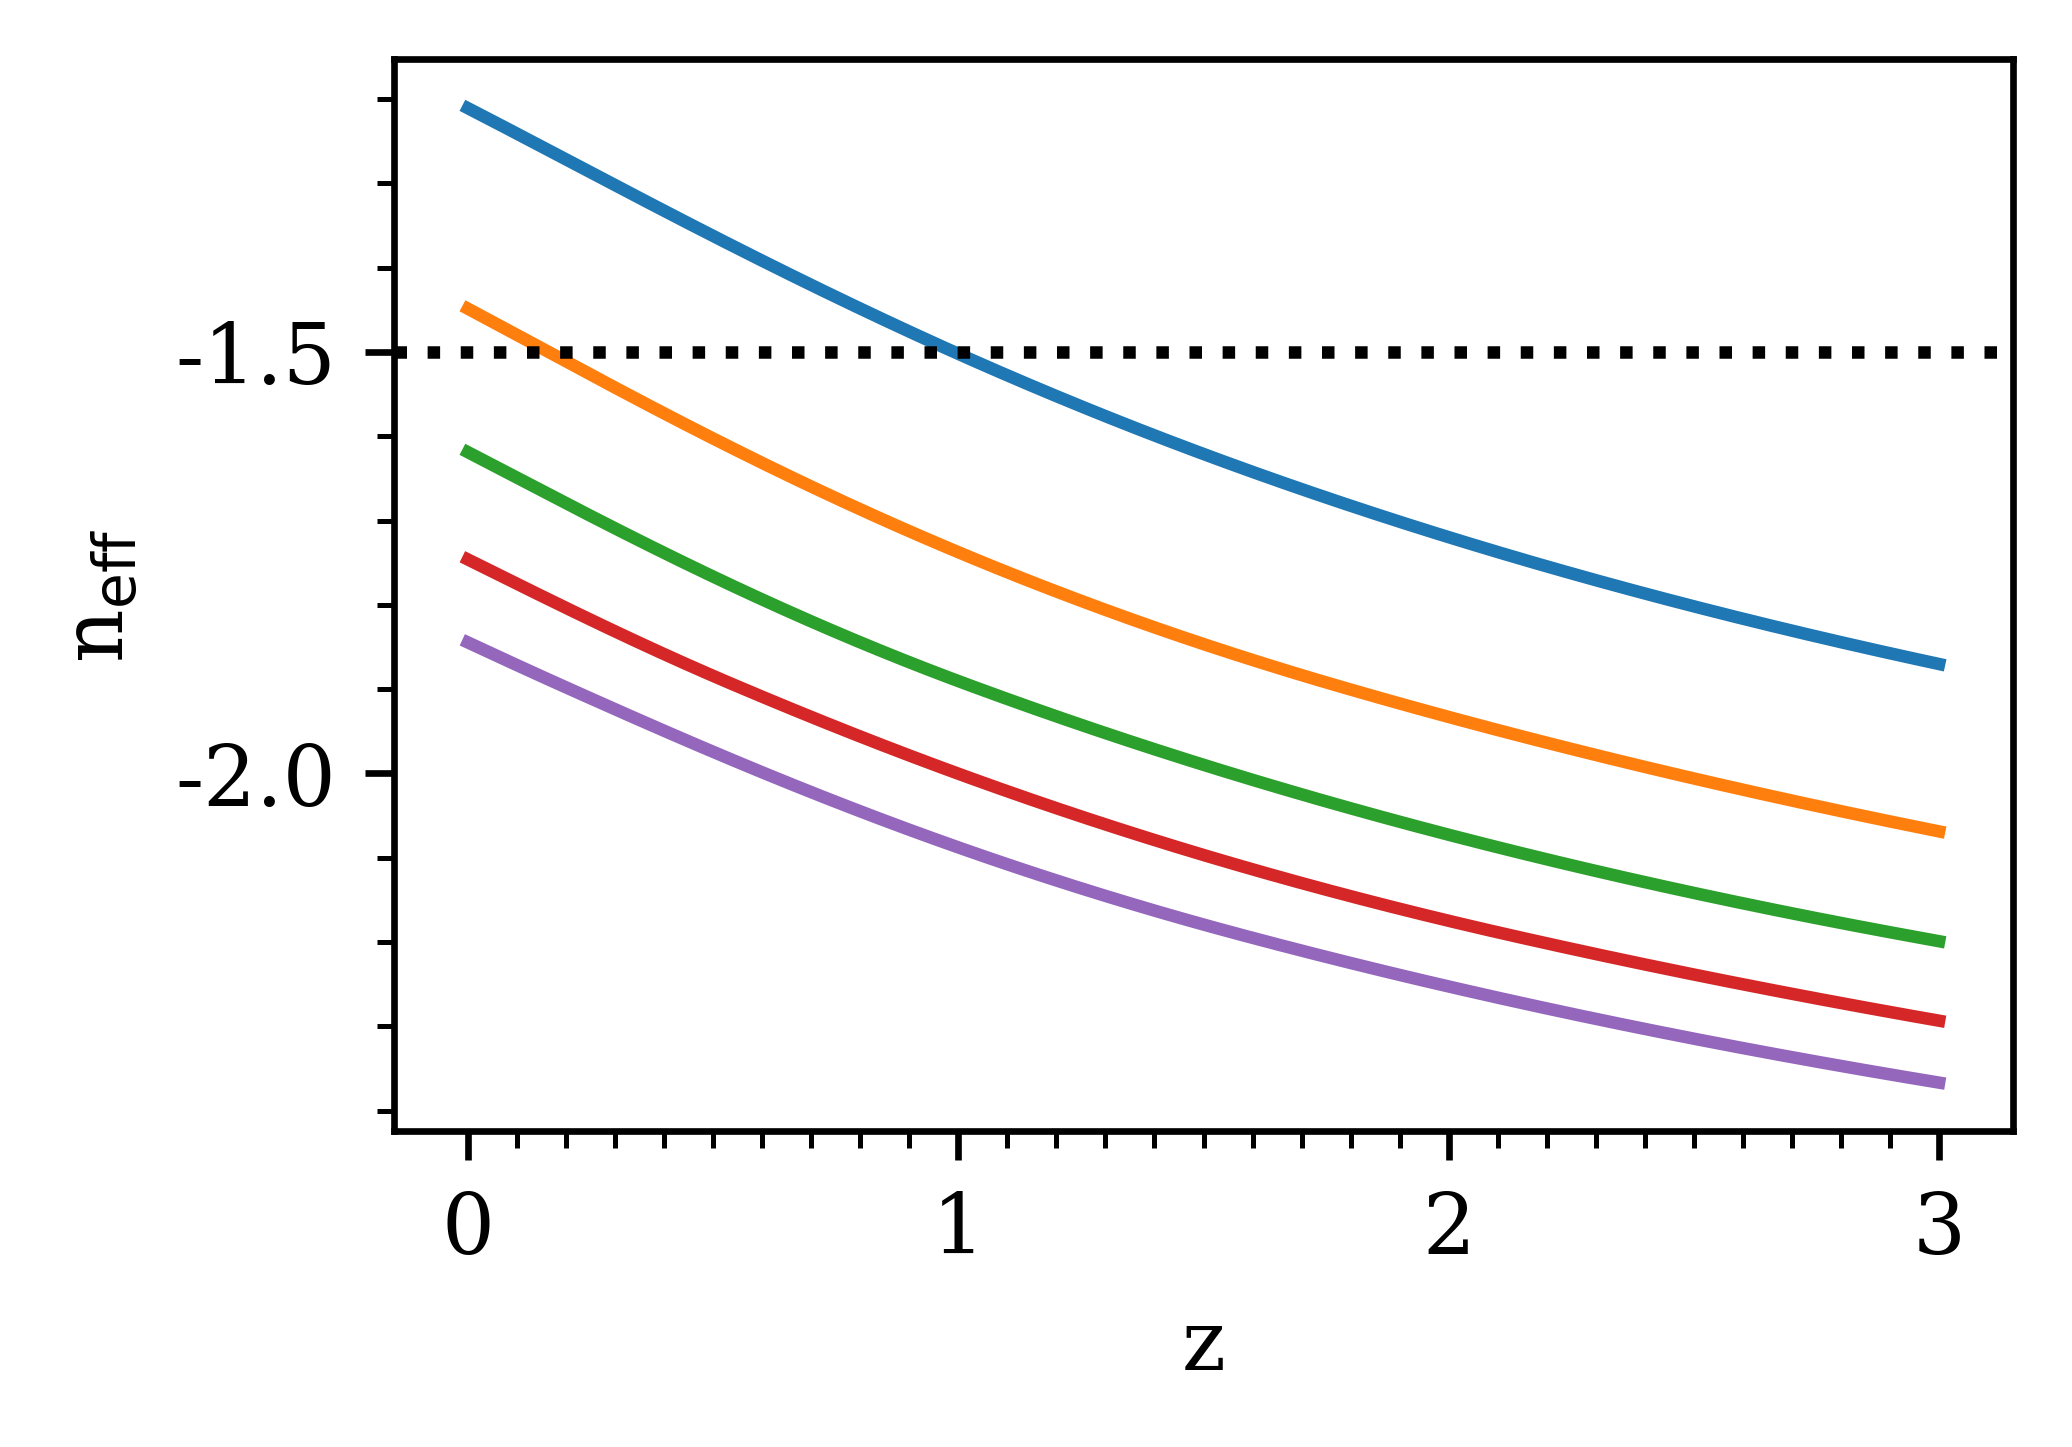
\includegraphics[width=\textwidth]{Ch3_Self_Sim/Paper_Plots_gtr20/n_eff_vs_z_sigma_plots.png}
\caption{}
\end{subfigure}
\hfil
\begin{subfigure}{.49\textwidth}
\centering
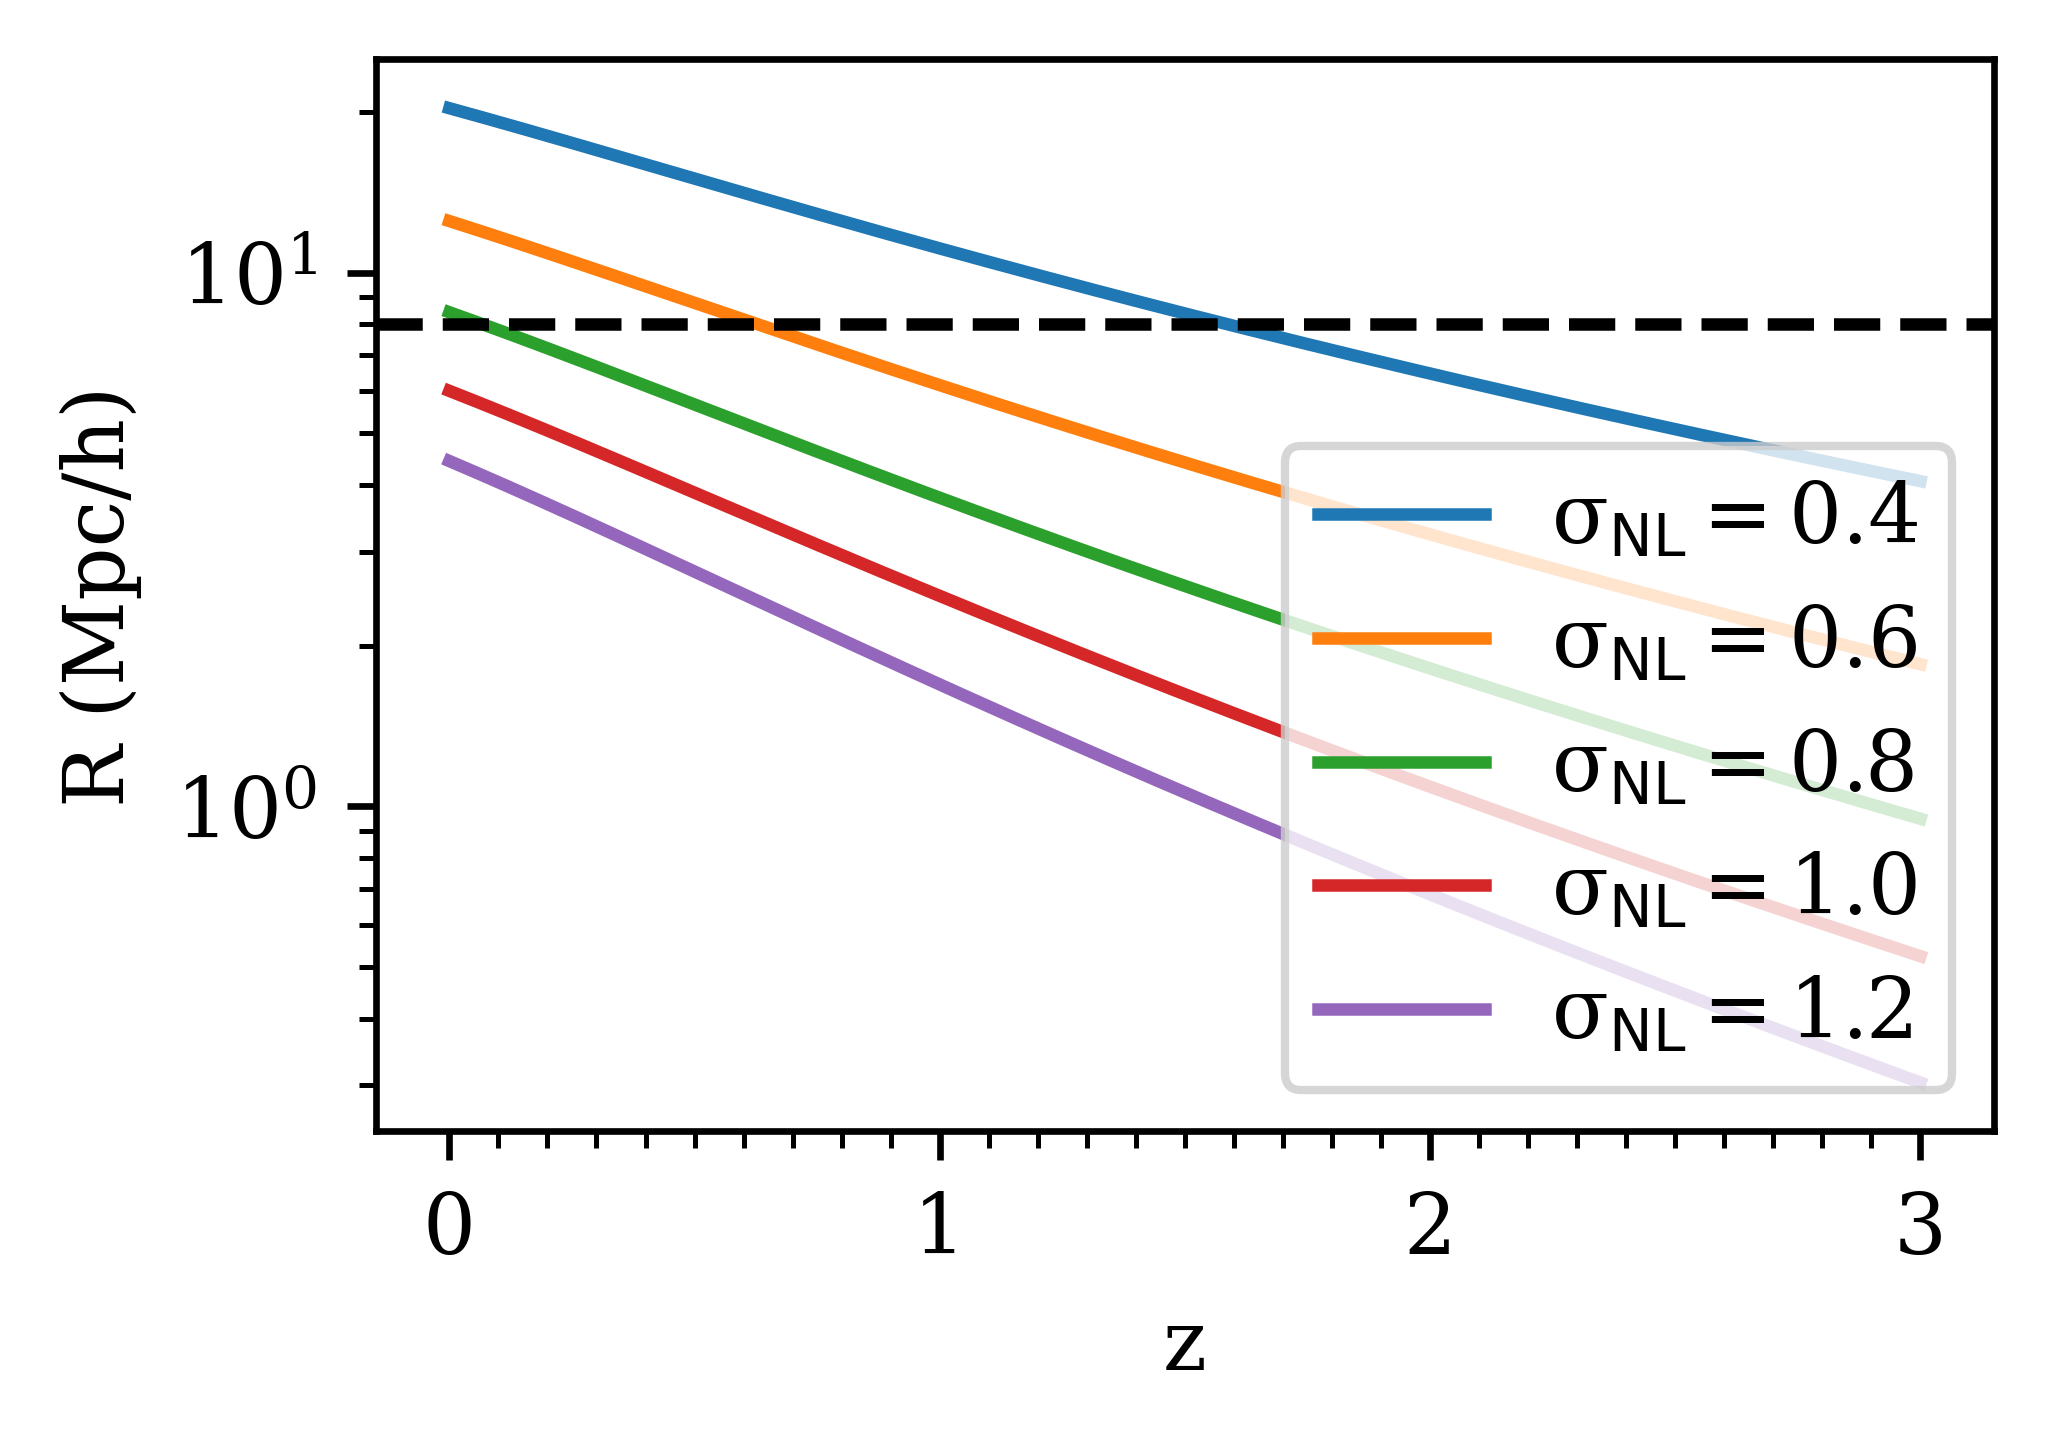
\includegraphics[width=\textwidth]{Ch3_Self_Sim/Paper_Plots_gtr20/R_vs_z_sigma_plots.png}
\caption{}
\end{subfigure}
\caption{\raggedright Plots of the effective spectral index, $n_{\mathrm{eff}}$, and scale, $R$, for a given linear top-hat variance, $\sigma_{\mathrm{lin}}\left(R, a\right) = \sigma_{\mathrm{NL}}$. Plots were made using \textsc{Colossus} \cite{Colossus}, with a \textit{Planck} 2018 cosmology \cite{Planck_2018_Cosmo}. The dotted line in plot (a) corresponds to $n_{\mathrm{eff}}=-1.5$ and the dashed line in plot (b) corresponds to $R = 8$ Mpc/$h$. The variance $\sigma_{\mathrm{NL}}$ provides a means of relating a scale and redshift in $\Lambda$CDM to a scale-free cosmology. We find that an effective spectral index of $n_{\mathrm{eff}}=-1.5$ implies a length scale of 11.15 Mpc/$h$ and a Lagrangian mass of $\sim5\times10^{14} M_{\odot}/h$, which in turn corresponds to the Lagrangian length and mass scale we expect for cluster-sized halos.}
\label{fig:n_eff_plots}
\end{figure*}

The initial amplitude of Gaussian fluctuations was $\sigma(\ell, a_i) = 0.03$. The time step parameter is $\eta_\mathrm{acc} = 0.15$ \cite[see][for further discussion]{Joyce_2021}. The initial conditions of the simulation use \textsc{Abacus}'s second-order Lagrangian perturbation theory (2LPT) implementation and particle linear theory (PLT) corrections \cite{Garrison_2016}. Our simulation uses a spline force softening scheme \cite[see descriptions in][]{Garrison_2016} with a Plummer-equivalent length of $\ell/30$ \cite{Plummer_1911}. The impacts of the softening scheme were explored in previous works \cite[e.g.,][]{Garrison_2021_softening, Maleubre_2022}. 

We define the first output of the simulation, as in previous work, as the approximate scale factor ($a_0$) at which non-linear structures begin to form (i.e., $\sigma_{\mathrm{lin}}(\ell, a_0) = 0.56$). The subsequent simulation snapshots are spaced by a factor of $\sqrt{2}$ in the non-linear mass scale. From Equation \ref{eqn:nonlinearmass}, we find that
\begin{equation}\label{eqn:log_a_spacing}
    \Delta \log_2(a) = \frac{3 + n}{6} \Delta \log_2(M_{\mathrm{NL}}) = \frac{3+n}{12}.
\end{equation}
As a result, we can represent the time as evenly spaced points representing the doubling of the scale factor since $a_0$ using $\log_2(a/a_0)$. This has the benefit of describing the simulation in more universal terms that are then applicable to other simulations (see Section \ref{LCDM}). We examine 30 snapshots from the simulation. For a more comprehensive description of the \textsc{Abacus} $N$-body code simulation used, we refer the reader to \cite{Maleubre_2024}, and to previous works which explored the convergence of various parameter choices \cite[][]{Joyce_2021, Garrison_2021_softening, Maleubre_2022}.

\subsection{Halo Finders: \textsc{CompaSO} and \textsc{Rockstar}}\label{finders_descriptions}
In this study we test our simulation with two halo finders, the Robust Overdensity Calculation using K-Space Topologically Adaptive Refinement (\textsc{Rockstar}) \cite{Rockstar} and \textsc{CompaSO} \cite{CompaSO}. To calculate the mass accretion histories we need, we pair \textsc{Rockstar} with the merger tree algorithm \textsc{Consistent Trees} \cite{Consistent_trees} and we apply a cleaning procedure to \textsc{CompaSO} \cite{CompaSO_Merger_Trees}. In the following subsections we describe the halo finding and merger tree creation procedures of each algorithm.

\textsc{Rockstar} identifies halos with the following procedure. First, it uses a friends-of-friends algorithm \cite{FoF} to determine overdense groups of particles in the simulation volume. The normalized phase space information of each group is used to iteratively define subgroups, such that at each step 70\% of particles are linked together in subgroups. Seed halos are then placed at the deepest level of subgroup, with particles in higher subgroups assigned to the nearest halo in phase space. For an illustrated summary of this procedure, see figure 1 in \cite{Rockstar}. 

\textsc{Consistent Trees} constructs a merger tree using \textsc{Rockstar} halos, evolving the simulation backwards in time to create a consistent merger history. The initial stage does this by identifying, and sometimes creating, progenitor halos. First, it uses the positions and velocities of halos to predict their locations at the previous time step. Using that information, it then eliminates spurious progenitor-descendant relationships while identifying likely ones. Additionally, it creates progenitor halos, known as phantom halos, out of existing particles for halos with no identifiable progenitor. It also eliminates any halos without descendants that are too isolated to have been merged with another halo. 

The second stage of \textsc{Consistent Trees} focuses on eliminating bad merger trees. It removes massive halos with too high a proportion of particles coming from the aforementioned phantom halos. It also removes massive halos and subhalos that do not exist for a sufficient number of time steps. For a more in depth summary of \textsc{Consistent Trees}, see section 5 of \cite{Consistent_trees}. To construct our mass accretion histories, we use the default $M_{200c}$ mass definition from \textsc{Consistent Trees}. We identify the most massive progenitors of distinct (non-subhalo) halos. We do so by looking only at clusters with \texttt{pid} $< -1$ and then matching past halos to their descendants by comparing \texttt{desc\_id} to \texttt{id}. By selecting only unique matches or the match with most massive progenitor, we are able to construct our mass accretion histories. We limit our analysis to halos with at least 20 particles, but the phantom halos generated in \textsc{Consistent Trees} procedure go down to as low as a few particles.


\textsc{CompaSO} determines halos in three stages. Before identifying halos, a local density is estimated at each particle location using a kernel width of $0.4\ell$, where $\ell$ is again the initial particle spacing. Particles with a sufficiently high local density are grouped into what are called L0 groups, using a friends-of-friends algorithm. Within each L0 group, a set of halos, L1 halos, are calculated. The particle with the peak local density inside an L0 group is treated as the nucleus of an L1 halo. Particles are tentatively assigned to the L1 halo if they fall within a radius determined with a threshold density. This L1 identification process is then repeated using all particles that fall outside 80\% of the L1 radius. In this case the nucleus of any additional L1 halos is required to have a local density greater than all particles within some predefined radius. Particles are assigned to these additional L1 halos if they were previous unassigned or if their enclosed density with respect to the new nucleus is twice that of the their enclosed density with respect to the nucleus of the previously assigned halo. This process is repeated until a minimum density threshold is reached. Finally, subhalos, called L2 halos, are identified for each L1 halo. They are assigned using the L1 halo identification method, but within a given L1 halo. Note that \textsc{CompaSO} imposes a strict $30$ particle cutoff for halos.

Merger trees are constructed and cleaned using the procedure described in \cite{CompaSO_Merger_Trees}. The algorithm does so by tracing a subsample of 10\% of the particles in a halo across time. Starting with some L1 halo, the algorithm looks back one previous time step and identifies all L1 halos that existed within $4$ Mpc. Using this list of halos, a list of candidate progenitors is made by evaluating which historical halos have a non-zero fraction of particles from the current halo. If the fraction of particles in the candidate shared between the candidate and the current halo is above the threshold fraction, the candidate is considered a progenitor. The progenitor halo that contributes the most particles to the current halo is called the main progenitor. This procedure is completed for halos two time steps back in time from the current time, but only the main progenitor is recorded, and is referred to as the main progenitor preceding. This procedure is repeated for all halos at all times where a sufficient number of time steps are available. There is an additional cleaning procedure, analogous to the second stage of \textsc{Consistent Trees}. For a given halo at time $z_i$, the algorithm identifies a redshift, $z_{\mathrm{max}}$, at which the halo on the main progenitor branch of the current halo reaches its greatest mass. If this greatest mass is sufficiently larger than the mass of the current halo, the current halo is flagged for cleaning. The flagged halo is merged with a contemporaneous neighboring halo that is the most massive descendant of the maximum mass main progenitor identified at $z_{\mathrm{max}}$. The combined halo then remains combined for all future time steps. The effect of this procedure is to reduce the breaking up of larger halos inflicted by the stricter spherical over density cuts imposed by the primary \textsc{CompaSO} procedure. \cite{Maleubre_2024} demonstrated that the cleaning procedure improved convergence to self-similarity in the halo mass function. We do not directly test the impact of omitting the cleaning procedure in this work, however in Section \ref{compaso_results} we discuss the ways in which differences in \textsc{CompaSO} and its cleaning procedure as compared to \textsc{Rockstar} and \textsc{Consistent Trees} might impact the preservation of self-similarity.

With \textsc{Rockstar} we are able to retrieve halo data for all 30 simulation snapshots, and therefore can analyze the mean mass accretion history information of 29 snapshots. When using halo data from \textsc{CompaSO}, due to an issue with the data, we are limited to 27 snapshots of halos, and therefore 26 snapshots of mass accretion history information. 

\section{Results}\label{ch3_results}
\subsection{\textsc{Rockstar}}\label{rockstar_results}


\begin{figure*}
\centering
\begin{subfigure}{.49\textwidth}
\centering
\includegraphics[width=\textwidth]{Ch3_Self_Sim/Paper_Plots_gtr20/Rockstar15_mean_past_joyce_mah_M200c_gtr20_FW_WW5_M_M_NL_vs_a_convergence_MT2_UVM_min_1000.png}
\caption{\textsc{Rockstar} Convergence\\ vs Rescaled Mass}
\end{subfigure}
\hfil
\begin{subfigure}{.49\textwidth}
\centering
\includegraphics[width=\textwidth]{Ch3_Self_Sim/Paper_Plots_gtr20/Rockstar_n15_mean_past_joyce_mah_M200c_gtr20_FW_WW5_N_vs_a_convergence_MT2_UVM_min_1000.png}
\caption{\textsc{Rockstar} Convergence\\ vs Halo Particle Count}
\end{subfigure}
\caption{\raggedright Plots of the convergence of mass accretion histories, calculated using the \textsc{Rockstar} halo finder are shown. In plot (a) the convergence is plotted as a function of the rescaled mass bin ($M/M_{\mathrm{NL}}$) and the doubling factor of the scale factor since the first halos collapsed ($\log_{2} \left(a/a_0\right)$). Plot (b) shows the same convergence, but replaces the rescaled mass bin with the particle count per halo ($N$). This transformation is possible using the second definition of $M_{\mathrm{NL}}$ in Equation \ref{eqn:nonlinearmass}. From plot (b), one can get a sense of the bounds of convergence. Convergence is strongest when $\log_2(a/a_0) \geq 2$. Within that time frame, the converged particle count varies from $\sim  20$ to $\sim 2\times10^4$. Centered in this area, there is a concave region of convergence, with a continuous region of high (1\%) convergence that is surrounded by smaller shells of lesser convergence. The very upper bounds of convergence, in terms of particle count, are near $10^5$. This upper bound of convergence at late times appears when the halo population limit ($> 1000$ halos) is reached, so it is probable that the limit is imposed by the finite volume of the simulation, and not the halo finder. The lower bound of convergence demonstrates interesting temporal behavior. At very early times, $\log_2 (a/a_0) \sim 0.5$, 2\% convergence is observed. Immediately following this the lower bound of convergence is pushed up to $N\sim10^2$. Convergence then begins to reach lower particle counts, before reaching the minimum lower bound of $N=20$ at $\log_2 (a/a_0) = 3$. Beyond this point, our choice of convergence window width begins to influence our ability to measure convergence, and no further convergence is measured. A full analysis of this behavior can be found in Section \ref{rockstar_results}.}
\label{fig:Rockstar_convergence}
\end{figure*}


Figure \ref{fig:Rockstar_convergence} displays the results of our convergence procedure using halos found with \textsc{Rockstar}. The results demonstrate a remarkable range of robustness for our definition of mass accretion history, with halos ranging from a few tens of particles to nearly 100,000 particles demonstrating 2\% convergence to self-similarity. The region of highest convergence is found at late times ($\leq 1$\% at $\log_2(a/a_0) \geq 2$). At its greatest extent, when the scale factor is roughly eight times the scale factor at non-linear collapse ($a_0$), the region of high convergence stretches almost continuously from as low as a couple hundred particles to as high as $\sim 20,000$ particles. 

It is unsurprising that the most massive halos ($\gtrsim1000$ particles) demonstrate greater convergence at later times. The hierarchical nature of structure formation means that larger structures take longer to form. As a consequence, as the simulation evolves, the number of very massive halos grows. Since we require there to be more than 1000 halos for a region to be probed, an increase in the number of very massive halos at later times allows new regions of parameter space to be probed. The depth of convergence for more massive halos is similarly improved by their increased number. The mass accretion history we use is a mean of a distribution. When the population of halos is low, that distribution, which can be thought of as a random sample of an underlying distribution of possible mass accretion histories for halos of that rescaled mass bin, will be noisier. This noisiness will prevent higher levels of convergence. However, as the population of very massive halos grows, the noisiness of the sample of the mass accretion history distribution decreases, and thus convergence to self-similarity is more likely. Therefore, when using \textsc{Rockstar}, the convergence limits of the most massive halos are dictated by the finite box size of the simulation, not the properties of the halo finder itself. Finally, it is worth noting that halo masses in this simulation are discrete. More massive halos therefore have an advantage in achieving convergence over less massive halos, as their increased masses mean that the integer mass of halos has a less prominent effect on the possible mass accretion histories available to a halo.

For intermediate masses ($\sim100-1000$), similar reasoning explains the improvement in convergence over time. At very early times intermediate mass halos are drawn from the exponential tail of the halo mass function. In this region, there are very few halos of similar mass. This sparsity makes the mean mass accretion history noisy. At later times intermediate mass halos are drawn from the power-law regime of the halo mass function, meaning there are many halos of similar mass, thus stabilizing the mean mass accretion history. At early times the intermediate mass halos are some of the most massive halos in the simulation and therefore are relatively isolated. At late times there are large populations of small ($<100$) and large ($>1000$) halos. This means that for all intermediate mass halos there is a sufficiently large population of halos to accrete mass from, and to be accreted on to, to avoid being dominated by numerical effects.

Beyond illustrating the simulation and halo finder's deep fidelity to self-similarity, Figure \ref{fig:Rockstar_convergence} also reveals interesting convergence behavior for low mass halos. At very early times, there is an isolated region of 2\% convergence, that then disappears entirely. This behavior is explored further in Figure \ref{fig:Rockstar_Transient_Convergence}. The evidence suggests that the sudden appearance and disappearance of 2\% convergence is an artifact of the choice convergence window width (see Fig.~\ref{fig:rockstar_vary_window_N_v_a_convergence}.) However, there is some level of real convergence to self-similarity underlying that behavior. At early times, low particle count halos of the same rescaled mass bin fall within a tight range of mean mass accretion histories, demonstrating the flatness behavior discussed in Section \ref{self_similarity}. To understand this, one must consider the behavior holistically. The long term trend of mean mass accretion histories, for all evaluated rescaled mass bins and times, is to decrease as the simulation evolves forward in time. At very early times, the mass accretion history distribution is dominated by very massive accretors and comparatively fewer negative accretors. As the simulation evolves, this balances shifts, with comparatively fewer extreme positive accretors, more negative accretors, and many more small but positive accretors. It appears that for relatively small halos at early times, the change in extreme positive accretors vs negative accretors is sufficiently balanced to stabilize the mean and create the appearance of convergence. Given the uncertainty around this behavior, we consider this region of convergence to be dubious.

\begin{figure*}
\centering
\begin{subfigure}{.49\textwidth}
\centering
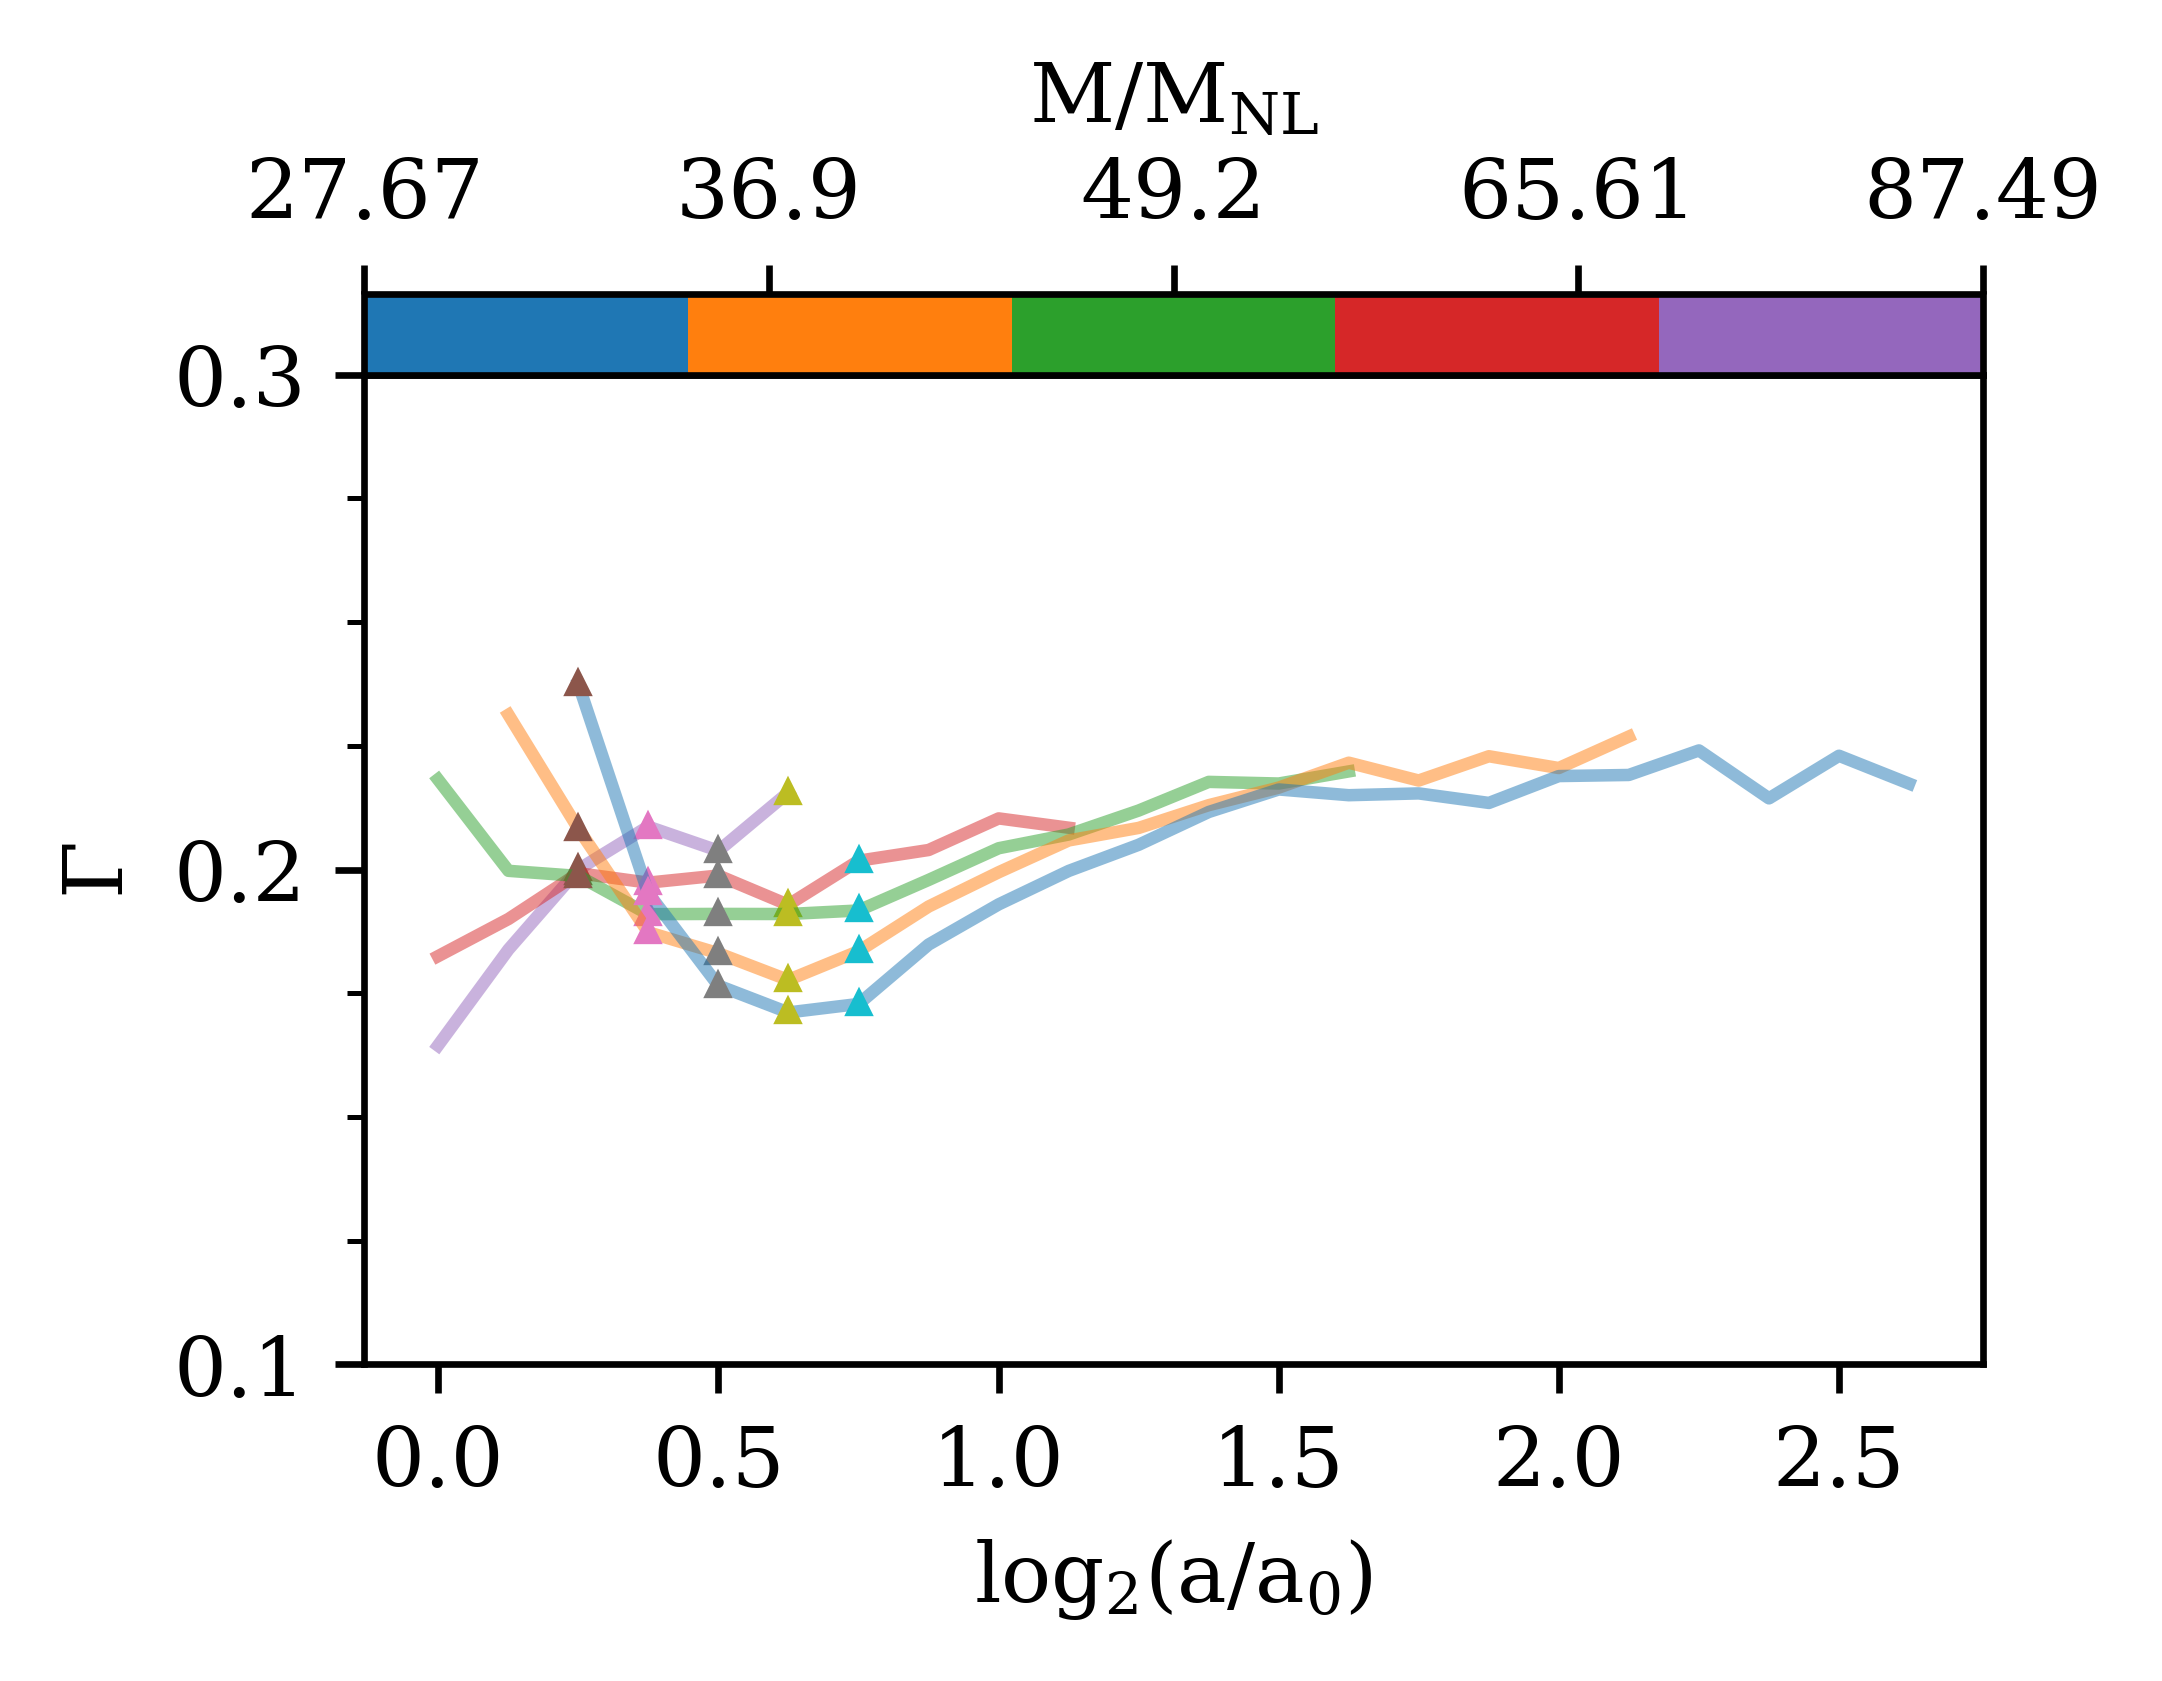
\includegraphics[width=\textwidth]{Ch3_Self_Sim/Paper_Plots_gtr20/M200c_gtr20_ROCKSTAR_n15_z_mean_mah_vs_a_early_time_investigation_050824.png}
\caption{Mean mass accretion histories\\ of 5 high $M/M_{NL}$ bins}
\end{subfigure}
\hfil
\begin{subfigure}{.49\textwidth}
\centering
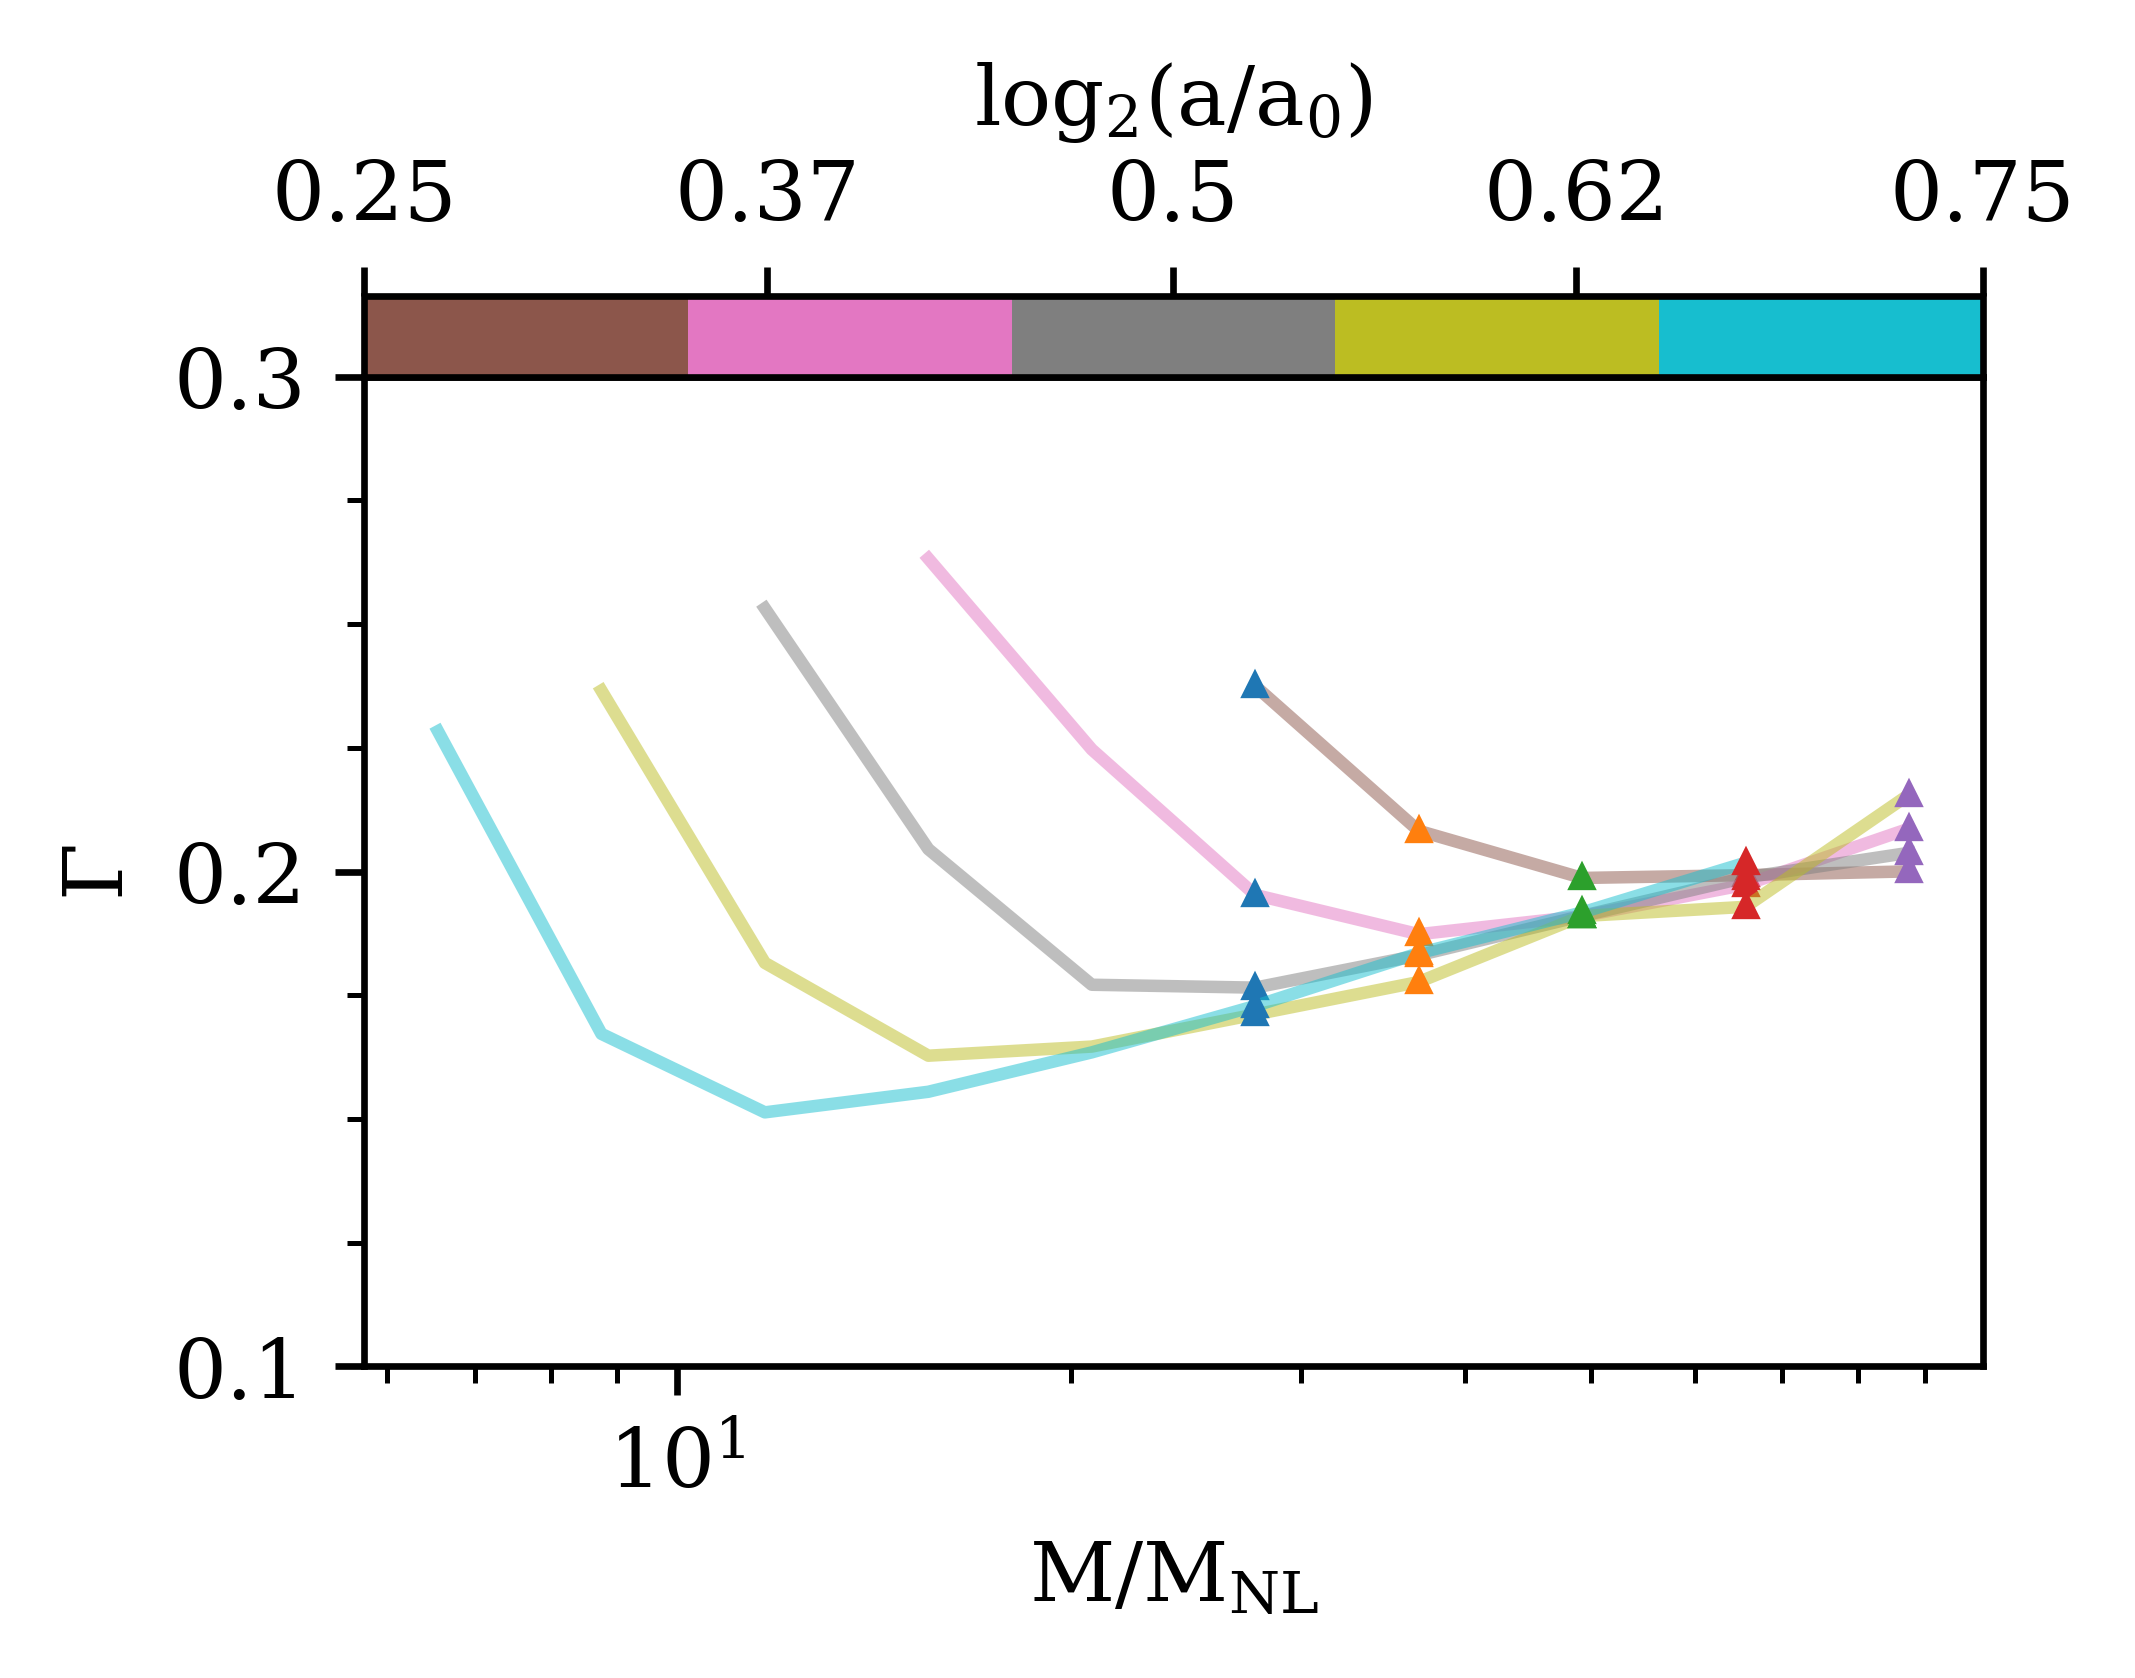
\includegraphics[width=\textwidth]{Ch3_Self_Sim/Paper_Plots_gtr20/M200c_gtr20_ROCKSTAR_n15_z_mean_mah_vs_M_M_NL_early_time_investigation_050824.png}
\caption{Mean mass accretion history\\ of 5 early snapshots}
\end{subfigure}
\caption{\raggedright  Above are plots illustrating the mass accretion histories of low mass halos in the early time 2\% convergence region for halos found using \textsc{Rockstar}. Plot (a), in the style of Figure \ref{fig:Rockstar_CompaSO_mah_v_a}, shows the mean mass accretion history ($\Gamma$) of five rescaled mass bins, as a function of time (in units of the doubling of the scale factor since $a_0$). The triangles indicate the 5 times probed. Plot (b), like Figures \ref{fig:rescaling_example} and \ref{fig:CompaSO_rescaling_example}, shows the mean mass accretion history of the 5 snapshots as a function of rescaled mass bin. Here the triangles indicate the 5 rescaled mass bins probed. The chosen combination of rescaled mass bins and snapshots corresponds to the top left corner of Figure \ref{fig:Rockstar_convergence} (a), which in turn corresponds to the bottom left corner of plot (b) of the same figure. In plot (a) we can see the early region of flatness that drives the 2\% convergence on the green line. We can also see how that flatness appears out of a smooth transition in the shape of the $\Gamma$ curve. For the highest $M/M_{NL}$ bin shown (purple), $\Gamma$ starts lower and transitions to higher values at later times. As the $M/M_{NL}$ bin decreases, what was once a bump (purple) in $\Gamma$ at $log_2 (a/a_0)\sim0.5$ flattens (green) before becoming a dip (blue). We can also see that a new, later region of flatness appears near $log_2 (a/a_0)\sim1.5$. Taken together, we can see that there is a brief region of apparent self-similarity at early times. This region disappears as a later region of self-similarity appears with a different mean mass accretion history value. Since the early region of apparent self-similarity is transitory, and, more importantly, converges to a different value than later times, we view it as dubious. We discuss a possible reason for this pseudo-convergence in Section \ref{rockstar_results}.}
\label{fig:Rockstar_Transient_Convergence}
\end{figure*}

Convergence at very low particle counts is not observed again until much later times, by which point the scale factor has quadrupled. This convergence develops gradually and continuously, starting at higher particle count halos at earlier times and gradually reaching very low mass halos at later times.  It is possible that the softening length, which gets smaller in comoving coordinates as the simulation evolves, is improving convergence \cite{Garrison_2021_softening}. Similarly, as the simulation evolves with time, it may begin to lose its memory of the initial lattice of particles \cite[see][for further discussion]{Joyce_2021, Maleubre_2022}. At very late times ($\log_2(a/a_0)\geq3$), we are limited not by the simulation or the halo finder, but by the convergence estimation procedure itself. As seen most clearly in Figure \ref{fig:Rockstar_convergence} (a), for the lowest mass halos at late times, there are less than five time steps available at a given rescaled mass bin. Since our procedure limits us to regions of stability at least five snapshots wide, we are unable to probe these regions. Alternative convergence metrics, explored in Appendix \ref{alternative_convergence_metrics}, imply that these unexplored regions also are converged.

\subsection{\textsc{CompaSO}}\label{compaso_results}
Figure \ref{fig:CompaSO_convergence} illustrates our results for halos found using \textsc{CompaSO}. We can see that there is a region of high ($\leq2$\%) convergence at late times ($\log_2 (a/a_0) > 2$), ranging from several hundred to a few thousand particles per halo. Like with the \textsc{Rockstar} results, this late time convergence is likely driven by sufficient evolution away from the non-physical length scales introduced in the initial conditions of the simulation.

The bounds of convergence, both of the $\leq2$\% region, and of the much larger $\leq10$\% region, are driven by the choice of halo finder. \textsc{CompaSO} imposes a strict spherical overdensity definition for identifying halos and their constituent particles. The \textsc{CompaSO} cleaning procedure, as described in Section \ref{finders_descriptions}, attempts to correct this behavior by re-identifying some small neighboring halos and flyby halos as being part of their larger neighbors. This cleaning procedure, while needed, is insufficient to preserve the robustness of the mass accretion history of very large halos. The upper bound of convergence in Figure \ref{fig:CompaSO_convergence} demonstrates a nearly flat, in particle count per halo space, cutoff for high mass halos. Beyond this point halos are too large, and too diffuse at high radii, and therefore inappropriately broken up by \textsc{CompaSO}'s halo identification procedure. Similarly, it is possible that the cleaning procedure, in re-identifying some small halos as being simply subhalos of a larger halo, is incorrectly destroying what should be independent halos. This could also be imposing the bound on convergence for low mass halos. In the case of the low mass halos, another important barrier to low mass convergence is the 30 particle limit for halos, which is 10 particles greater than the limit we impose on the \textsc{Rockstar} results.

Despite these limitations, the \textsc{CompaSO} results still demonstrate convergence over an impressive range in time and particle count. The convergence of sub-100 particle halos is consistent from $a\sim \sqrt{2}a_0$ to very late times. The loss of convergence for very late times above this $\sim 50$ particle boundary is, like in the \textsc{Rockstar} case, driven by our choice of window width in determining convergence (as is evident in Figures \ref{fig:compaso_vary_window_N_v_a_convergence} and \ref{fig:tapered_tail_N_v_a_convergence} in appendix \ref{alternative_convergence_metrics}). Similarly, when not limited by the number of available high mass halos, there is a stable boundary of convergence at $\sim5000$ particles per halo. This convergence upper bound is similar to that found in \cite{Maleubre_2024}.

\begin{figure*}
\centering
\begin{subfigure}{.49\textwidth}
\centering
\includegraphics[width=\textwidth]{Ch3_Self_Sim/Paper_Plots_gtr20/CompaSO15_mean_past_joyce_mah_M200c_gtr20_FW_WW5_M_M_NL_vs_a_convergence_MT2_UVM_min_1000.png}
\caption{\textsc{CompaSO} Convergence vs\\ Rescaled Mass}
\end{subfigure}
\hfil
\begin{subfigure}{.49\textwidth}
\centering
\includegraphics[width=\textwidth]{Ch3_Self_Sim/Paper_Plots_gtr20/CompaSO_n15_mean_past_joyce_mah_M200c_gtr20_FW_WW5_N_vs_a_convergence_MT2_UVM_min_1000.png}
\caption{\textsc{CompaSO} Convergence vs\\ halo particle count}
\end{subfigure}
\caption{\raggedright Above are plots similar to those shown in Figure \ref{fig:Rockstar_convergence}, but for mass accretion histories obtained using the \textsc{CompaSO} halo finder. A region of high convergence, albeit lower than that seen in Figure \ref{fig:Rockstar_convergence}, is visible for $\log_2(a/a_0) > 2$. The range of particle counts at which 2\% convergence achieved is approximately $5\times10^2$ to $6\times10^3$. The small size of this region is partially imposed by a clear upper bound in convergence at $N\sim10^4$, well below the limit imposed by the limited very high mass halo population of the simulation. The lower bound of convergence does not display as obvious a time evolution as seen in Figure \ref{fig:Rockstar_convergence}. Instead, there is a mostly flat lower bound of 10\% convergence at $N\sim50-60$. The 5\% convergence does display time evolution, however, with convergence reaching lower particle counts as $\log_2(a/a_0)$ goes from $1$ to $\gtrsim2$. Convergence also appears to weaken past $\log_2(a/a_0)\gtrsim3$. Further analysis can be found in Section \ref{compaso_results} and Section \ref{comparing_finders}.}
\label{fig:CompaSO_convergence}
\end{figure*}

\section{Discussion}\label{ch3_discussion}
\subsection{Comparing Halo Finders}\label{comparing_finders}
Like in \cite{Maleubre_2024}, we find that \textsc{Rockstar} generally preserves self-similarity better than \textsc{CompaSO}. While the results for both halo finders show a region of high convergence in roughly the same particle count versus scale factor size space, the depth and breadth of convergence for \textsc{Rockstar} is greater. \textsc{Rockstar} also demonstrates a superior convergence for very high mass halos at late times, for the reasons discussed in Section \ref{compaso_results}. \textsc{Rockstar} also has superior convergence for low mass halos at late times, as seen in Figure \ref{fig:lower_bounds}.


\begin{figure*}
\centering
\begin{subfigure}{.49\textwidth}
\centering
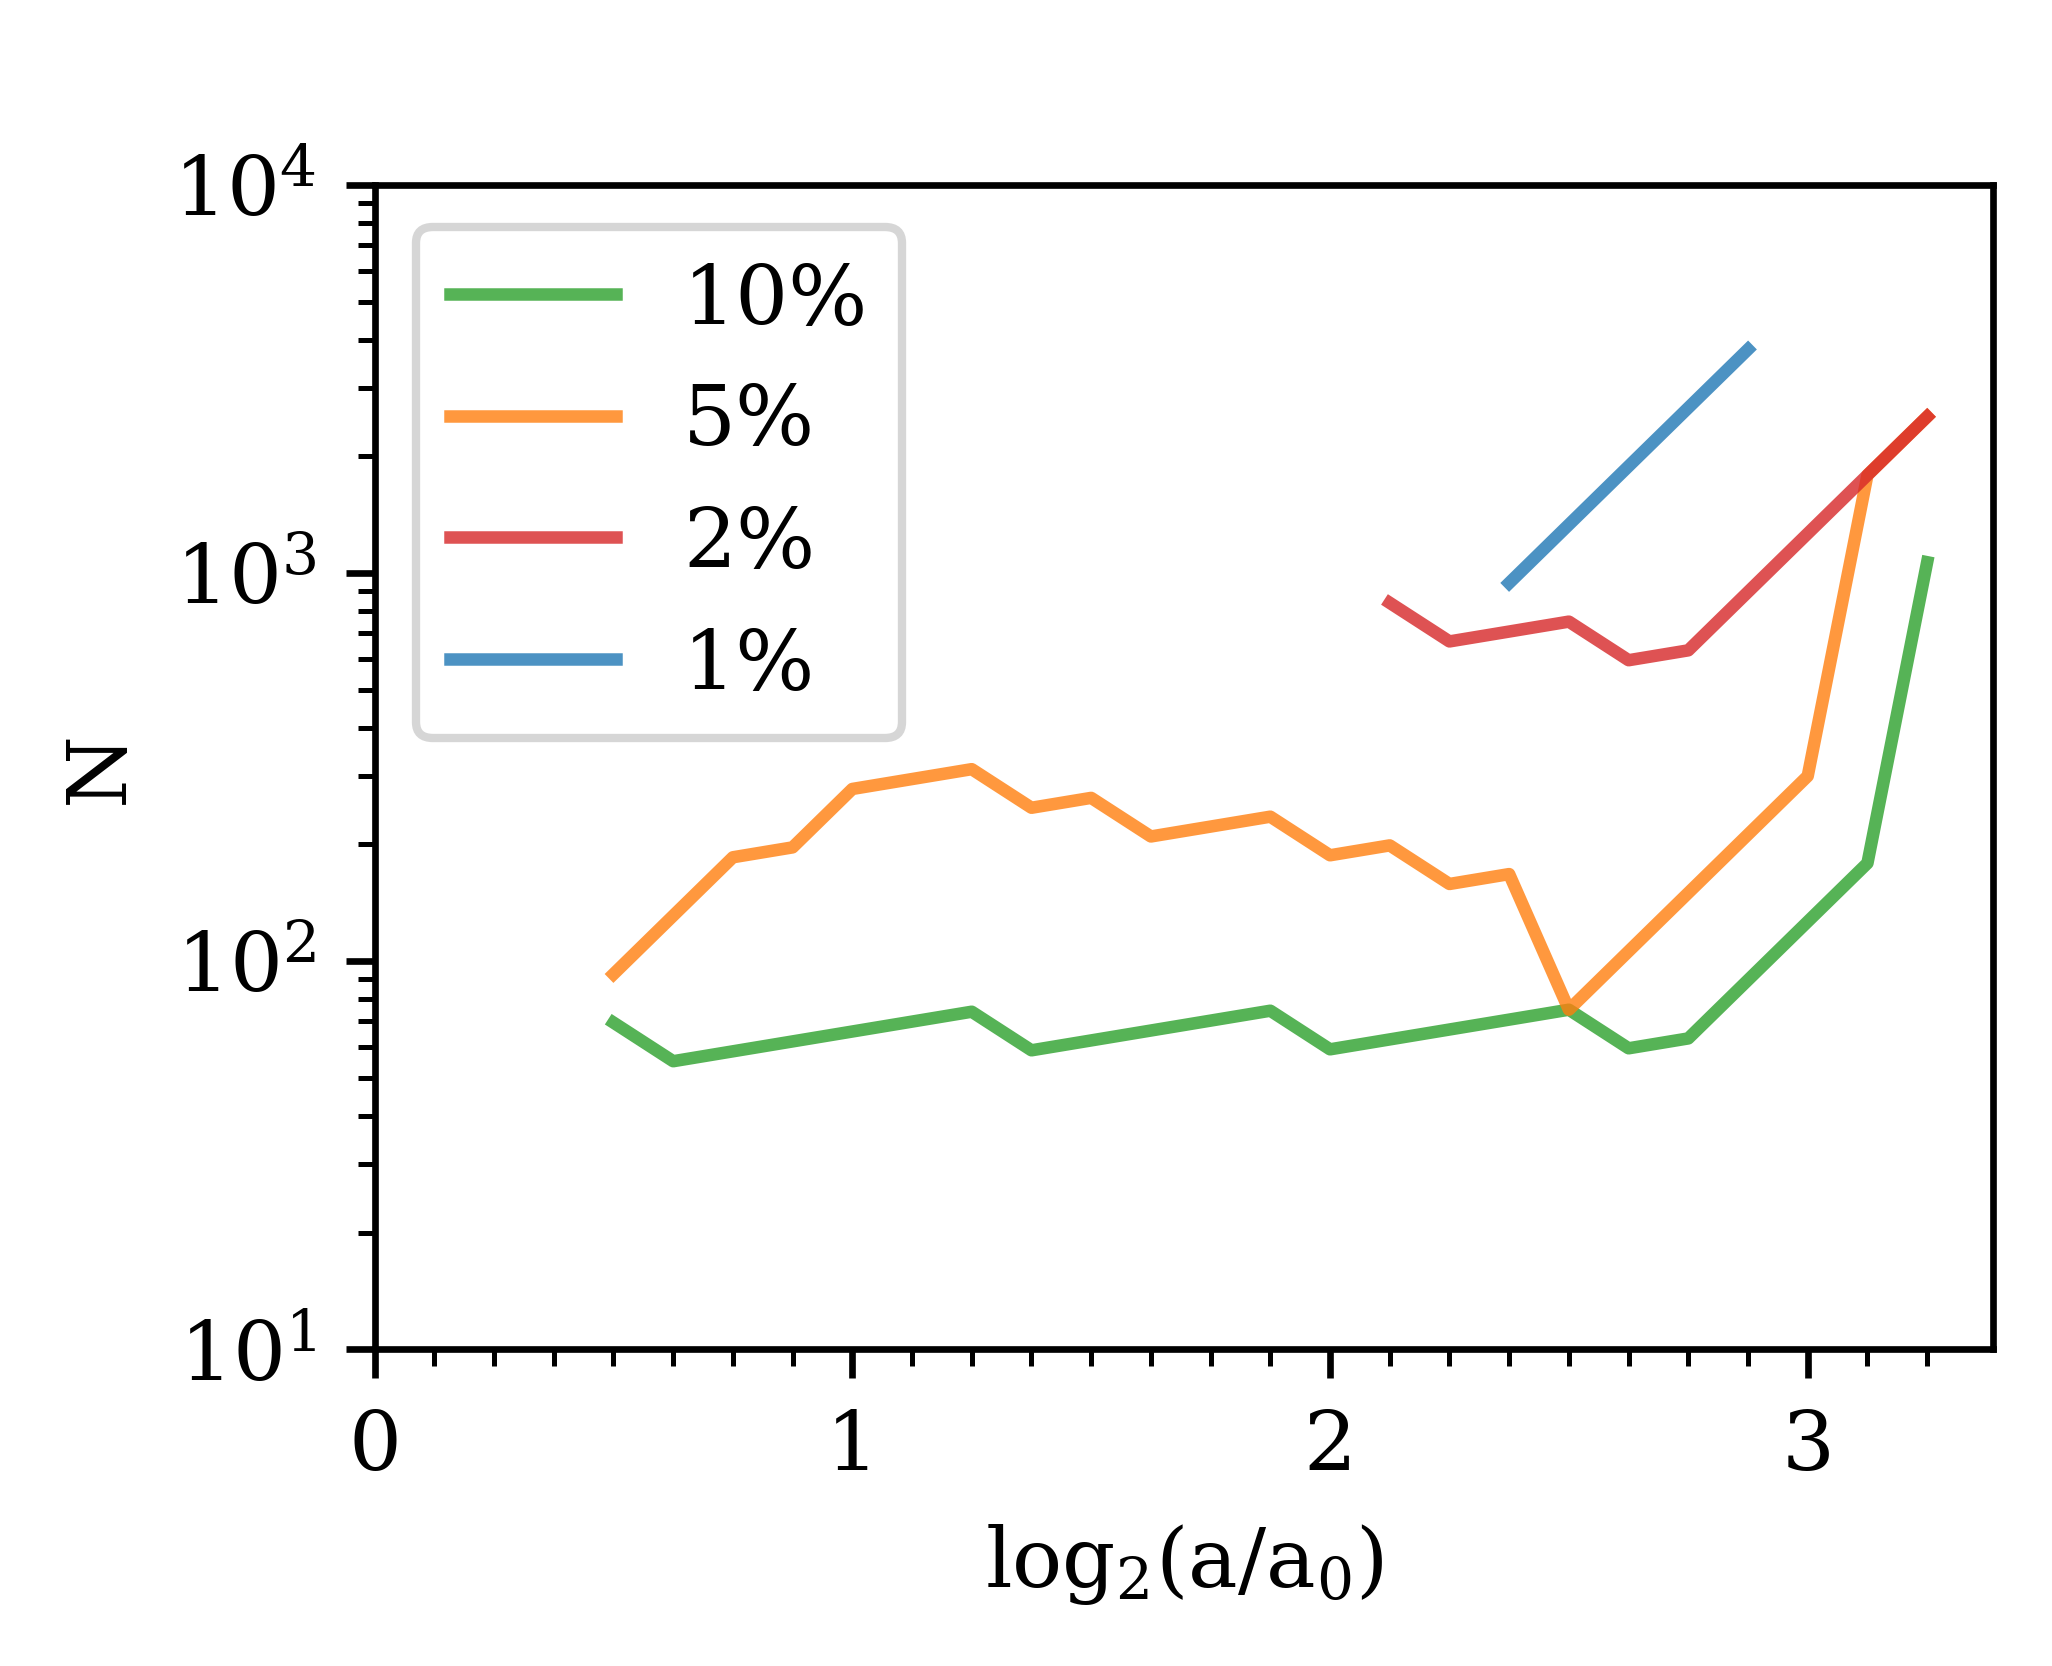
\includegraphics[width=\textwidth]{Ch3_Self_Sim/Paper_Plots_gtr20/M200c_gtr20_COMPASO_n15_N_mins_default_convergence_metric_no_concavity_meanD1_050824.png}
\caption{\textsc{CompaSO}}
\end{subfigure}
\hfil
\begin{subfigure}{.49\textwidth}
\centering
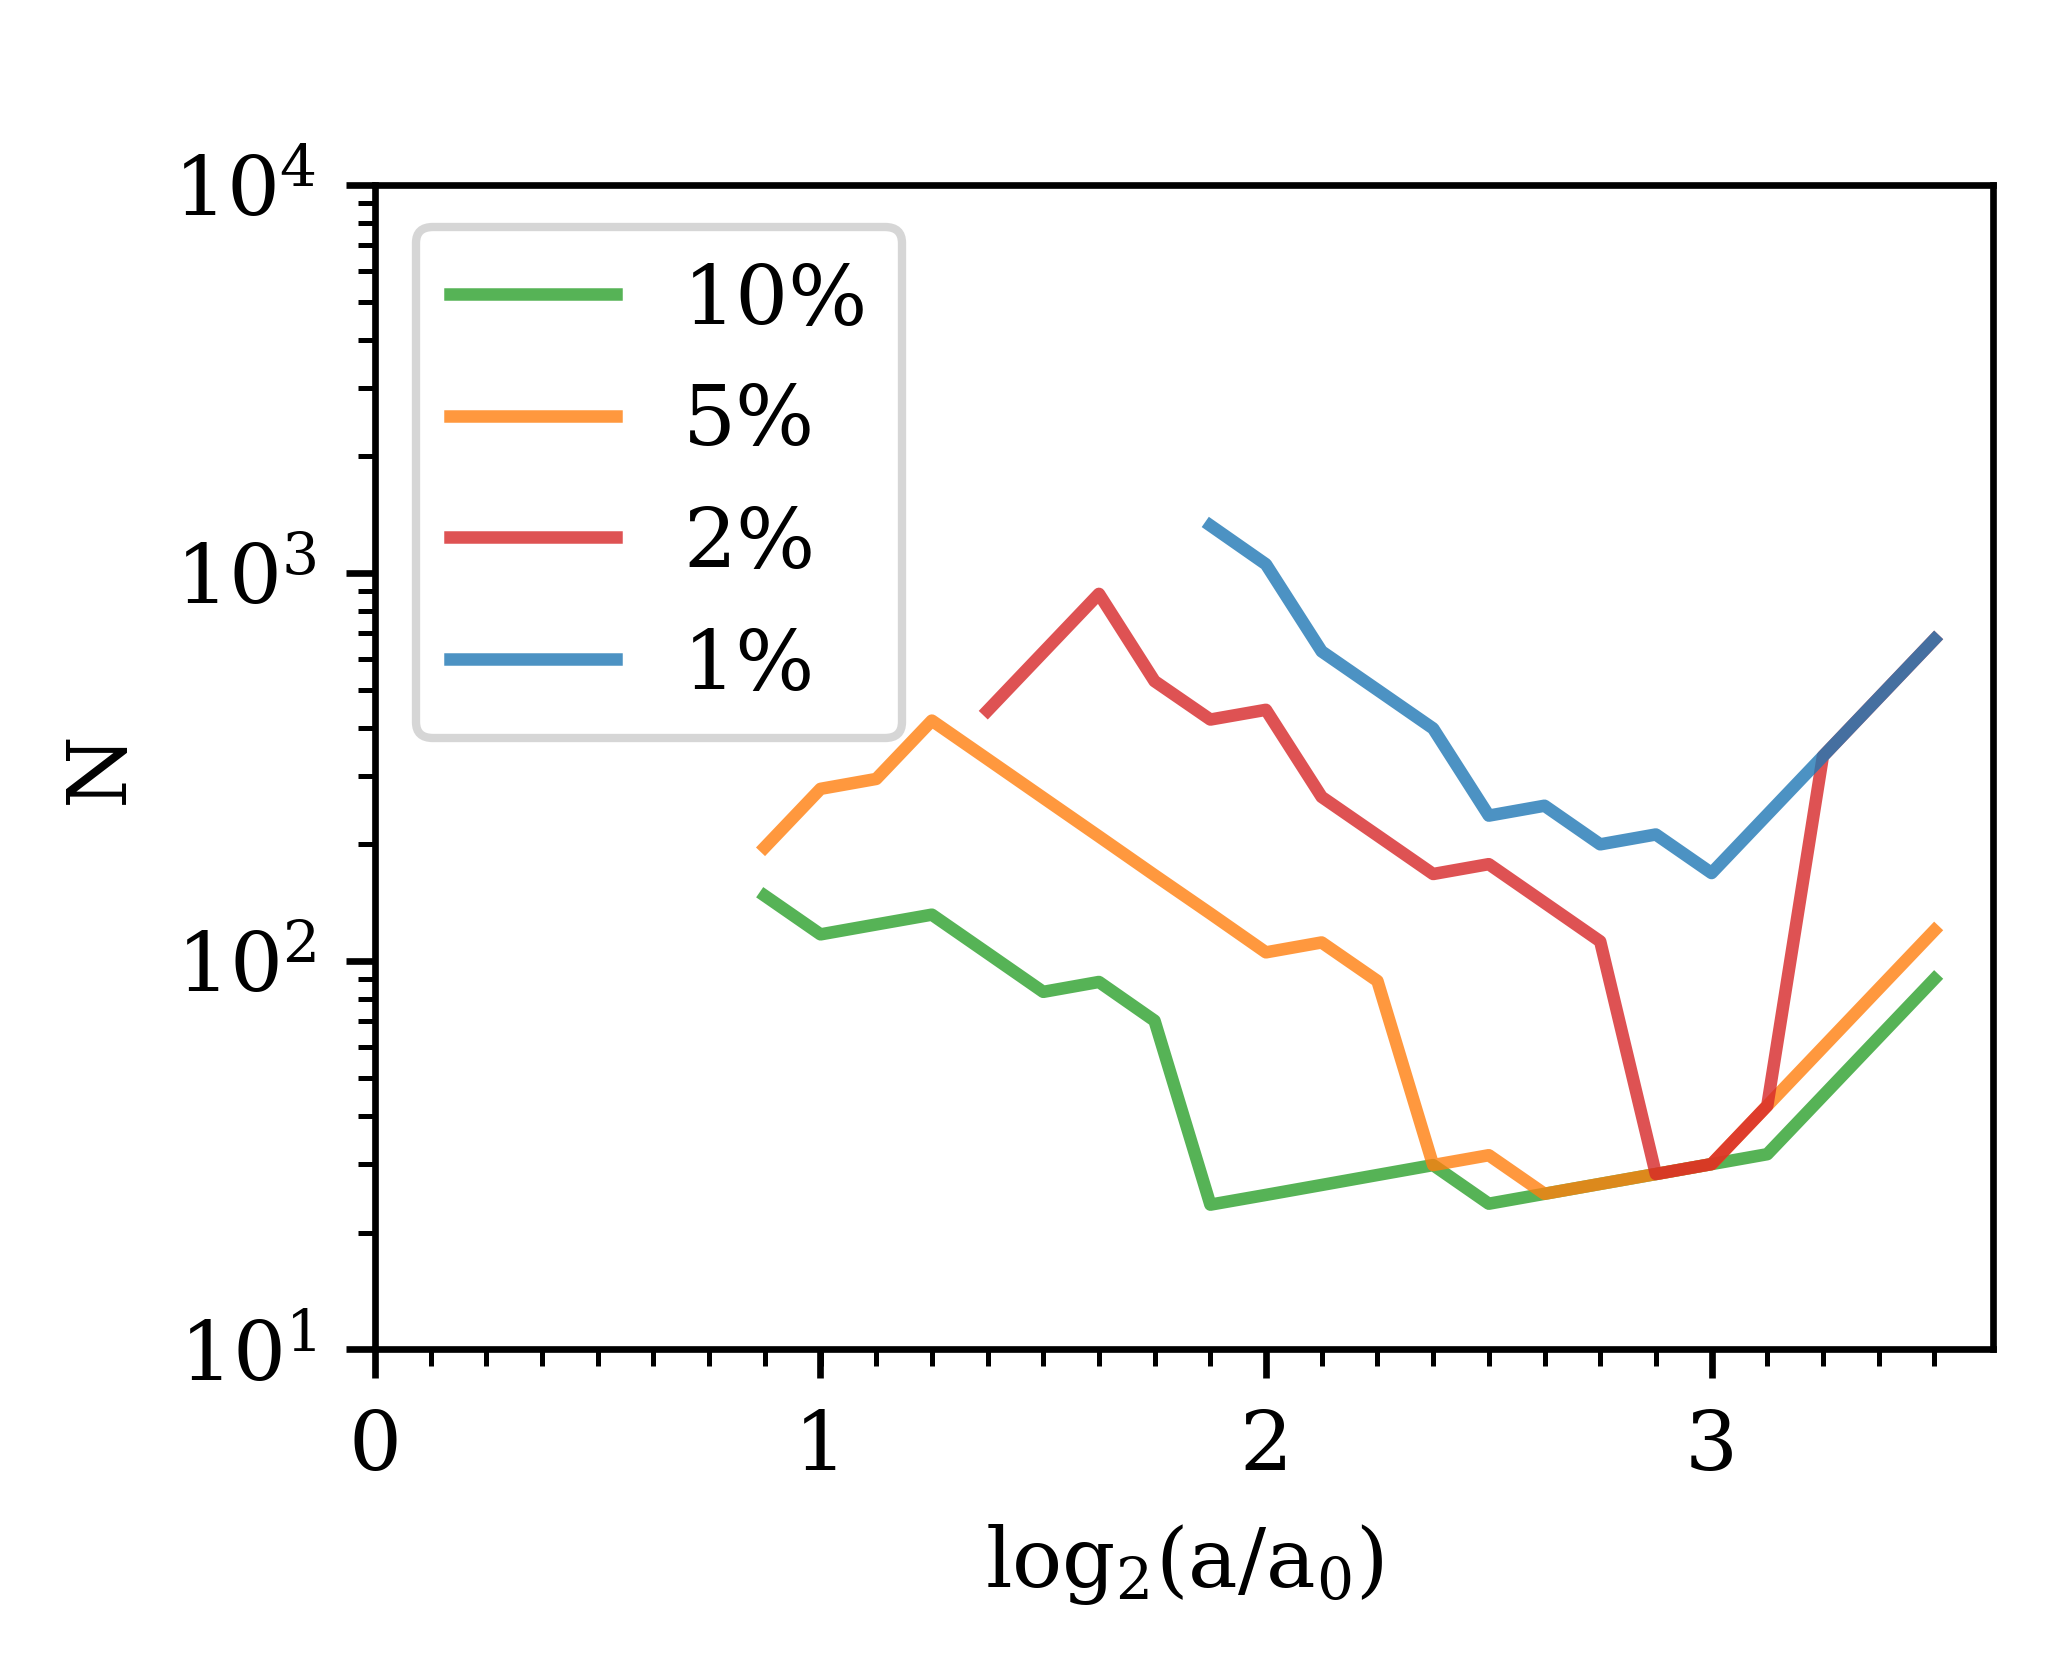
\includegraphics[width=\textwidth]{Ch3_Self_Sim/Paper_Plots_gtr20/M200c_gtr20_ROCKSTAR_n15_N_mins_default_convergence_metric_no_concavity_meanD1_050824.png}
\caption{\textsc{Rockstar}}
\end{subfigure}
\caption{\raggedright Above are plots of the \textsc{CompaSO} and \textsc{Rockstar} convergence lower bounds. For a given snapshot, the convergence lower bound is defined as the lowest particle mass at which $X$\% of convergence is achieved. Furthermore, we require there to be some continuity, meaning that more massive halos within the snapshot must also be converged to the same level. Finally, we remove the very early time convergence salient for \textsc{Rockstar}, for the reasons discussed in Section \ref{rockstar_results} and Figure \ref{fig:Rockstar_Transient_Convergence}. The lower bound plots illustrate that \textsc{Rockstar} obtains much better convergence at later times. We also see that \textsc{CompaSO} does not demonstrate the same intensity in the evolution of convergence for low mass halos. Instead we see a modest time evolution in the 5\% convergence and no time evolution for 10\% convergence. We discuss why \textsc{CompaSO} has weaker low mass convergence in Section \ref{compaso_results}.}
\label{fig:lower_bounds}
\end{figure*}

While \textsc{Rockstar} has a number of advantages with regards to mass accretion history fidelity, \textsc{CompaSO} has an absolute advantage in terms of computational cost and speed. Given this difference in computational cost, it is not difficult to imagine scenarios where \textsc{CompaSO}'s sub-optimal convergence is preferable. In said cases, our results suggest that \textsc{CompaSO}'s mass accretion histories are safest when used for sizeable late time halos. Less conservatively, halos with between a few thousand and roughly one hundred particles are converged. 

It is important to note that we cannot make absolute claims as to which halo finder is more physically accurate. This analysis, in determining deviations from self-similarity, is able to determine the resolutions at which the halo finder is no longer reliable. Testing the physical accuracy of the halo finders, or the simulation itself, requires a combination of scale-free validation, non-scale-free validation, and comparing simulated observables to real observables.

\subsection{Applications to Non Scale-Free Cosmologies}\label{LCDM}
While the convergence bounds provided by this work were found using only a single simulation and two halo finders, the results can be applied more broadly. The redshift dependent results of this work are presented as a function of $a/a_0$. Given the initial particle spacing $\ell$, one can use our definition of $a_0$ (see Section \ref{Abacus}) to determine $a_0$ for any other simulation. With this information, we can apply our results to $\Lambda$CDM simulations on sufficiently large scales such that the effective spectral index is $n_{\mathrm{eff}}\sim-1.5$. As discussed in Section \ref{Abacus}, this means our results are already applicable as an upper bound to galaxy cluster scales in other simulations. To apply our results more broadly still, we would need to explore the dependence of mean mass accretion history convergence as a function of the initial power spectrum. Preliminary work suggests that changing the spectral index has a real but minor impact on the convergence limits of the mean mass accretion history, but further work is needed. Comparing $n=-1.5$ and $n=-2.0$ results from \cite{Maleubre_2024} using the halo mass function also suggest that difference is minor. Therefore it is possible that our results are not strongly dependent on the initial conditions, and apply more generally to $\Lambda$CDM simulations.

A second possible caveat to this is that our results are derived from an EdS cosmology, thus one should be more cautious in applying our results to $\Lambda$CDM simulations near $z=0$, where deviations from EdS become more significant. Work by \cite{Joyce_2021} on the particle two-point correlation function (2PCF), suggested that the convergence of the 2PCF at small scales and late times might be cosmological model independent, and thus applicable to both a scale-free EdS simulation and a $\Lambda$CDM simulation at late times. In brief, the resolution of the 2PCF at small scales at late times is dominated by two-body scattering. This interaction is independent of the global properties of the simulation, and therefore cosmological model independent. Applying these conclusions to our work with the mean mass accretion history is less straightforward. The mean mass accretion history is by definition dependent on inter-halo interactions, and therefore the halo mass function, which is more sensitive to the choice of cosmological model. Work done by \cite{Maleubre_2024} using the halo-center 2PCF, which in principle would also depend on inter-halo interactions, suggests that the dependence on the cosmological model is weak, however. This suggests that our late time low mass results may indeed be nearly model independent, and therefore applicable even to low-redshift $\Lambda$CDM simulations.


\section{Conclusion}\label{ch3_conclusion}
In this work we probe the robustness of the halo mass accretion histories in a scale-free simulation generated using the \textsc{Abacus} $N$-body code. We do so by taking advantage of the expected self-similarity of dimensionless properties rescaled by the only physical scale in the simulation, the scale of non-linearity. We test the added effects on mass accretion robustness from the choice of halo finder, examining two different halo finders, \textsc{Rockstar} and \textsc{CompaSO}. We find that \textsc{Rockstar} demonstrates superior convergence than \textsc{CompaSO}. Both simulations demonstrate a wide range of convergence, with near 5\% convergence for the duration of the simulation for halos with particles counts as low as $\sim100$. This lower bound in particle count reduces further at late times, with an absolute minimum of $\sim70$ and $\sim30$ particles per halo demonstrating 5\% convergence for \textsc{CompaSO} and 2\% convergence for \textsc{Rockstar}, respectively. The upper bound particle limit also evolves with the simulation, reaching a maximum of $\sim10^4$ particles per halo when using \textsc{CompaSO} and maximum of $\sim10^5$ when using \textsc{Rockstar}. In \textsc{CompaSO} this upper limit appears to be a product of the limitations of the halo finder, but for \textsc{Rockstar} this upper bound occurs because the number of halos falls too low, suggesting we are limited by the finite volume of the simulation.

Halo mass accretion history is a key property for understanding galaxy clusters, and for using galaxy clusters to constrain cosmology. Much of the research into galaxy clusters and mass accretion history is reliant on cosmological simulations, and therefore in need of verification methods like the one discussed in this work. While the results of this work are easily applied to investigations of mass accretion history that use the \textsc{Abacus} $N$-body code, such as Warburton et al (in prep), the method used can be applied more broadly. Any code capable of creating a dark matter only simulation can be used to construct a scale-free simulation, which can then be probed using our method. Moreover, because \textsc{Abacus} is a highly accurate N-body code, the results here can be taken as the upper limit on possible convergence for other $N$-body codes, at least when using similar halo finding methods. Similarly, by taking advantage of our choice of spectral index, the results can provide limits of convergence on $\Lambda$CDM simulations at the galaxy cluster scale. By varying meta-parameters, like resolution and box size, as well as cosmological initial conditions, like spectral index, one can apply the convergence limits learned via this method to a variety of other cosmologies and scales. Our self-similarity test can also be applied to any other scale-free simulation and on other dimensionless clustering properties within a scale-free simulation. Doing so is essential to verifying the accuracy of state-of-the-art simulations, and therefore essential for verifying the inferences dependent on those simulations.

\section*{Data Availability}
Data access for the simulation part of \textsc{AbacusSummit} is available through OLCF’s Constellation Portal. The persistent DOI describing the data release is 10.13139/OLCF/1811689. Instructions for accessing the data are given at https://abacussummit.readthedocs.io/en/latest/data-access.html. The name of the simulation used in this work is ScaleFree\_v3\_N4096\_m15. The derived data generated in this research will be shared on reasonable request to the corresponding author.

\section*{Acknowledgments}

We thank Michael Joyce, Sara Maleubre Molinero, Sownak Bose, and Daniel Eisenstein for comments and suggestions for this work. Previous work on scale free simulations by them, like \cite{Maleubre_2024}, was also integral to this work. We also thank the Flatiron Institute Center for Computational Astrophysics Pre-Doctoral Program, which allowed for this collaboration.

The material presented is based upon work supported by NASA under award No. 80NSSC22K0821.

The simulations in this work used resources of the Oak Ridge Leadership Computing Facility (OLCF), which is a DOE Office of Science User Facility supported under Contract DE-AC05-00OR22725. The work was conducted under OLCF projects AST135 and AST145, the latter through the Department of Energy ALCC program. Most of the analysis was performed on computational resources supported by the Scientific Computing Core at Flatiron Institute, a division of Simons Foundation.


\section*{Appendix: Alternative Convergence Metrics}\label{alternative_convergence_metrics}
\subsection{Varying Convergence Window Widths}\label{varying_bin_width}


\begin{figure*}
\centering
\begin{subfigure}{.49\textwidth}
\centering
\includegraphics[width=\textwidth]{Ch3_Self_Sim/Appendix_Plots_gtr20/Rockstar_n15_mean_past_joyce_mah_M200c_gtr20_FW_WW4_N_vs_a_convergence_MT2_UVM_with_text_min_1000.png}
\caption{}
\end{subfigure}
\hfil
\begin{subfigure}{.49\textwidth}
\centering
\includegraphics[width=\textwidth]{Ch3_Self_Sim/Appendix_Plots_gtr20/Rockstar_n15_mean_past_joyce_mah_M200c_gtr20_FW_WW5_N_vs_a_convergence_MT2_UVM_with_text_min_1000.png}
\caption{}
\end{subfigure}
\begin{subfigure}{.49\textwidth}
\centering
\includegraphics[width=\textwidth]{Ch3_Self_Sim/Appendix_Plots_gtr20/Rockstar_n15_mean_past_joyce_mah_M200c_gtr20_FW_WW6_N_vs_a_convergence_MT2_UVM_with_text_min_1000.png}
\caption{}
\end{subfigure}
\caption{\raggedright Plots of the \textsc{Rockstar} convergence for different choices of window width in Equation \ref{eqn:delta1}. As discussed in Appendix \ref{varying_bin_width} and Section \ref{rockstar_results}, early time convergence is sensitive to changes in window width. The convergence regions produced using a four snapshot wide window are the noisiest, especially at higher particle counts. Here we suspect that a combination of lower halo counts and a heightened sensitivity to noise in the $\left<\Gamma\right>$ vs time curve are to blame. However, the differences between five and six snapshot wide widths is minimal, suggesting that some stability is achieved by five snapshots. In all cases the absolute lower and upper bounds of convergence remain the same.}
\label{fig:rockstar_vary_window_N_v_a_convergence}
\end{figure*}


\begin{figure*}
\centering
\begin{subfigure}{.49\textwidth}
\centering
\includegraphics[width=\textwidth]{Ch3_Self_Sim/Appendix_Plots_gtr20/CompaSO_n15_mean_past_joyce_mah_M200c_gtr20_FW_WW4_N_vs_a_convergence_MT2_UVM_with_text_min_1000.png}
\caption{}
\end{subfigure}
\hfil
\begin{subfigure}{.49\textwidth}
\centering
\includegraphics[width=\textwidth]{Ch3_Self_Sim/Appendix_Plots_gtr20/CompaSO_n15_mean_past_joyce_mah_M200c_gtr20_FW_WW5_N_vs_a_convergence_MT2_UVM_with_text_min_1000.png}
\caption{}
\end{subfigure}
\begin{subfigure}{.49\textwidth}
\centering
\includegraphics[width=\textwidth]{Ch3_Self_Sim/Appendix_Plots_gtr20/CompaSO_n15_mean_past_joyce_mah_M200c_gtr20_FW_WW6_N_vs_a_convergence_MT2_UVM_with_text_min_1000.png}
\caption{}
\end{subfigure}
\caption{\raggedright Plots of the \textsc{CompaSO} convergence for different choices of window width in Equation \ref{eqn:delta1}. As discussed in Appendix \ref{varying_bin_width}, early time convergence is sensitive to changes in window width. The depth of convergence in the region of high convergence is also effected by reducing the window width size to four, with the four width results suggesting more 1\% convergence. The general location of this region remains the same regardless of the choice of window width, however. In all cases the absolute lower and upper bounds of convergence remain the same.}
\label{fig:compaso_vary_window_N_v_a_convergence}
\end{figure*}

In Figures \ref{fig:rockstar_vary_window_N_v_a_convergence} and \ref{fig:compaso_vary_window_N_v_a_convergence} we compare the convergence results for different choices of $\Delta_1$ window width (see Section \ref{self_similarity}) for \textsc{Rockstar} and \textsc{CompaSO}. For both halo finders the general shape of the main region of convergence remains the same. Changes in convergence as a function of window width are most apparent at early times, where there are sometimes discontinuous regions of stability in the $\left<\Gamma\right>$ value (from Equation \ref{eqn:delta2}) as a function of time. This effect is most extreme when the size of the window is reduced, which creates islands of convergence for both halo finders. This sensitivity to our choice of metric suggests that this convergence is not robust. Moreover, as we argue in Section \ref{rockstar_results}, these early time regions of convergence should be treated with suspicion. Beyond these very early times, convergences regions are generally stable, with a reduction in window width size generating the most instability. This is unsurprising, given that with decreasing window width, our method becomes increasingly susceptible to noise.

\subsection{Tapered Tail Method}\label{tapered_tail}

\begin{figure*}
\centering
\begin{subfigure}{.49\textwidth}
\centering
\includegraphics[width=\textwidth]{Ch3_Self_Sim/Appendix_Plots_gtr20/Rockstar_n15_mean_past_joyce_mah_M200c_gtr20_FW_WW5_N_vs_a_convergence_MT2_UVM_with_text_min_1000.png}
\caption{\textsc{Rockstar}}
\end{subfigure}
\hfil
\begin{subfigure}{.49\textwidth}
\centering
\includegraphics[width=\textwidth]{Ch3_Self_Sim/Appendix_Plots_gtr20/Rockstar_n15_mean_past_joyce_mah_M200c_gtr20_TT_WW5_N_vs_a_convergence_MT2_UVM_with_text_min_1000.png}
\caption{\textsc{Rockstar}}
\end{subfigure}
\begin{subfigure}{.49\textwidth}
\centering
\includegraphics[width=\textwidth]{Ch3_Self_Sim/Appendix_Plots_gtr20/CompaSO_n15_mean_past_joyce_mah_M200c_gtr20_FW_WW5_N_vs_a_convergence_MT2_UVM_with_text_min_1000.png}
\caption{\textsc{CompaSO}}
\end{subfigure}
\begin{subfigure}{.49\textwidth}
\centering
\includegraphics[width=\textwidth]{Ch3_Self_Sim/Appendix_Plots_gtr20/CompaSO_n15_mean_past_joyce_mah_M200c_gtr20_TT_WW5_N_vs_a_convergence_MT2_UVM_with_text_min_1000.png}
\caption{\textsc{CompaSO}}
\end{subfigure}
\caption{\raggedright Plots comparing our chosen convergence metric to the "tapered tail" method discussed in Section \ref{tapered_tail}. The modified method allows us to probe lower particle counts at very late times, demonstrating the expected extension of convergence. It is more susceptible to \textsc{CompaSO}'s divergent behavior at high masses, however, and so we opt for our chosen method in the full in analysis.}
\label{fig:tapered_tail_N_v_a_convergence}
\end{figure*}

One observed consequence of our choice of convergence metric was our inability to probe very late times as effectively. At very late times there are not enough snapshots in the lowest rescaled mass bins to probe convergence. By relaxing our window width requirement at very late times, we can accommodate smaller numbers of bins and potentially probe these very late very low mass halos. We did so by setting the window width of Equation \ref{eqn:delta1} equal to five snapshots, or the number of remain snapshots, whichever is smaller. Since we calculate $\Delta_1$ sequentially from early times to late times, the effect of this is to calculate $\Delta_1$ for the last four, three, and two sufficiently populated snapshots of a given rescaled mass bin. Because the last snapshot is by itself, it automatically passes the first stage of the convergence test. The remaining steps of the convergence test are the same, including the requirement that there be at least three consecutive of snapshots of convergence for a given rescaled mass bin. So the major change is that the $\left<\Gamma\right>$ value in Equation \ref{eqn:delta2} is now calculated using the mean mass accretion history of the last available snapshot, as well as potentially the second, third, and fourth to last, as well as any other five-wide snapshot regions that passed the first convergence check.

In Figure \ref{fig:tapered_tail_N_v_a_convergence} we plot the convergence regions for our current convergence metric (in (a) and (c)) and this modified "tapered tail" method (in (b) and (d)). For \textsc{Rockstar}, this change of method has no major effect, but to continue the major region of convergence to lower particle counts at very late times. This very late time low particle improvement in convergence is repeated for the \textsc{CompaSO} results. \textsc{CompaSO}'s difficulty with very high mass halos causes problems for this method however. By relaxing the requirement window width at late times, we are effectively assuming that very late times always converge. This is true for all halos in \textsc{Rockstar}, but not true for large mass halos in \textsc{CompaSO} (see Figure \ref{fig:Rockstar_CompaSO_mah_v_a} for an example of \textsc{CompaSO}'s divergent behavior). When the window width is sufficiently reduced, the drop in mean mass accretion history for large mass halos at very late times is treated as a region of convergence. This dramatically skews the value of $\Delta_2$, obscuring any real convergence for smaller halos in that rescaled mass bin. In Figure \ref{fig:tapered_tail_N_v_a_convergence}, this is evident as a continuous break in the convergence region, extending from $\sim10^4$ particles per halo at $2^{2.5}\times a_0$ back down to $\sim10^3$ particles per halo at $2^{1.8}\times a_0$.
\subsection{Late Time Convergence}\label{low_z_convergence}
\begin{figure*}
\centering
\begin{subfigure}{.49\textwidth}
\centering
\includegraphics[width=\textwidth]{Ch3_Self_Sim/Appendix_Plots_gtr20/Rockstar_n15_mean_past_joyce_mah_M200c_gtr20_FW_WW5_N_vs_a_convergence_MT2_UVM_with_text_min_1000.png}
\caption{\textsc{Rockstar} with\\ Fixed 5 Width Window}
\end{subfigure}
\hfil
\begin{subfigure}{.49\textwidth}
\centering
\includegraphics[width=\textwidth]{Ch3_Self_Sim/Appendix_Plots_gtr20/Rockstar_n15_mean_past_joyce_mah_M200c_gtr20_LZ_N_vs_a_convergence_with_text_min_1000.png}
\caption{\textsc{Rockstar} with\\ Latest Time Convergence}
\end{subfigure}
\begin{subfigure}{.49\textwidth}
\centering
\includegraphics[width=\textwidth]{Ch3_Self_Sim/Appendix_Plots_gtr20/CompaSO_n15_mean_past_joyce_mah_M200c_gtr20_FW_WW5_N_vs_a_convergence_MT2_UVM_with_text_min_1000.png}
\caption{\textsc{CompaSO} with\\ Fixed 5 Width Window}
\end{subfigure}
\begin{subfigure}{.49\textwidth}
\centering
\includegraphics[width=\textwidth]{Ch3_Self_Sim/Appendix_Plots_gtr20/CompaSO_n15_mean_past_joyce_mah_M200c_gtr20_LZ_N_vs_a_convergence_with_text_min_1000.png}
\caption{\textsc{CompaSO} with\\ Latest Time Convergence}
\end{subfigure}
\end{figure*}
\begin{figure*}
\centering
\caption{\raggedright Above is a comparison of convergence procedures. The left column of plots (a and c) show our default procedure described in Section \ref{self_similarity}, while the right column (b and d) shows the results of the procedure described in Section \ref{low_z_convergence}. The top row (a and b) displays results produced using the \textsc{Rockstar} halo finder, while the bottom row (c and d) displays the results produced using \textsc{CompaSO}. The difference between (a) and (b) is less immediately obvious than the difference between (c) and (d). Both (b) and (a) have large regions of high (1\%) convergence, but region is pushed further back in time for (b). This difference is likely caused by the increased sensitivity of this method to noise and slow changes in $\Gamma$. The procedure for the default convergence metric will naturally set the converged $\Gamma$ (i.e. $\left<\Gamma\right>$ in Equation \ref{eqn:delta2}) to the average of all snapshots that pass $\Delta_1 \leq X\%$. On the other hand, the latest time convergence metric effectively sets $\left<\Gamma\right>=\Gamma\left(a_{\rm{max}}\right)$. This means that in instances where there is a gradual transition to flatness in the $\Gamma$ vs $\log_2 (a/a_0)$ curve, or where the final snapshot has a slightly deviant $\Gamma$ value, the default method will be more likely to find weaker convergence across a large region, whereas the latest time method will by default favor a smaller later region (assuming that region includes $\Gamma\left(a_{\rm{max}}\right)$) to the potential exclusion of any earlier snapshots. The case in which the regions of self-similarity do not contain $\Gamma\left(a_{\rm{max}}\right)$ is illustrated in the \textsc{CompaSO} results shown in (d). There, because of divergent behavior at late times, $\Gamma\left(a_{\rm{max}}\right)$ is rarely in a region of flatness. Therefore, using $\Gamma\left(a_{\rm{max}}\right)$ as a baseline, one rarely finds any convergence at all. It is exactly this flaw that dissuaded us from using this method in the main analysis, but we include it for completeness.}
\label{fig:low_z_convergence}
\end{figure*}

The last extension to our convergence metric that we considered was to do away with $\Delta_1$ entirely. Instead, we treated the mean mass accretion history of the latest sufficiently populated snapshot as the converged mean mass accretion history ($\left<\Gamma\right>$ in Equation \ref{eqn:delta2}). We then followed the same procedure (i.e., still requiring $\Delta_2 < X\%$ and still requiring three consective snapshots for a region of convergence). The results of this modified procedure are shown in Figure \ref{fig:low_z_convergence}. As expected, this procedure works well for \textsc{Rockstar}, where the mean mass accretion history of a rescaled mass bin converges to a single value as the scale factor increases. Equally as unsurprising, at least in light of the results in Section \ref{tapered_tail}, this result does not work at all for \textsc{CompaSO}. \textsc{CompaSO}'s difficulty with halos with $\gtrsim 10^4$ particles is amplified by this procedure. Because $M_{\mathrm{NL}}$ increases with time, the latest available snapshots of a given rescaled mass bin are also those containing the most massive halos. When these halos are sufficiently large, their mean mass accretion history as calculated by \textsc{CompaSO} diverges. Since this modified method uses these values as its benchmarks for convergence, this behavior totally obscures any convergence in rescaled mass bins where the halos get too large.

\chapter{A Multi-Wavelength Technique for Estimating Galaxy Cluster Mass Accretion Rates} \label{chap:chap-4}


\begin{singlespace}         % you can also use `onehalfspace` to relax the spacing
    This chapter is adapted from the following publication:
    
    \fullcite{Soltis_2025}. 
    %\mybibexclude{sol}
\end{singlespace} 

\section{Introduction}\label{Ch4_introduction}

Galaxy clusters, the most massive gravitationally bound objects in the Universe, contain collections of tens to thousands of galaxies. Galaxy clusters are roughly 80\% dark matter and 20\% ordinary matter. Of the ordinary matter, the vast majority is a hot, ionized gas known as the intra-cluster medium (ICM). Nearer to the cluster core, this ionized gas is X-ray bright \cite[e.g.,][]{Bulbul_2024}, emitting X-rays via bremsstrahlung, collisional excitation, recombination radiation, and 2-photon emission processes. The ICM is also observable from the inverse-Compton scattering of cosmic microwave background photons off the electrons in the ICM \cite[e.g.,][]{Hilton_2021}, an effect known as the thermal Sunyaev-Zeldovich (tSZ) effect \cite{SZ_1972}. As high density peaks of the mass distribution of the Universe, the abundance of galaxy clusters is sensitive to changes in cosmology \cite[e.g.,][]{eROSITA_Cluster_Abundances_2024}. Galaxy clusters are also an effective probe dark matter physics \cite[e.g.,][]{Andrade_2022} and astrophysics \cite[e.g.,][]{Fournier_2024}.

Galaxy clusters form by accreting dark matter, gas, galaxies, galaxy groups, and smaller galaxy clusters in their local environment \cite[for a review, see][]{Kravtsov_2012}. Simulations suggest that the formation history of a galaxy cluster influences its morphology substantially, including its concentration and shape of its density profile, its ellipticity, and the fraction of its mass contained within its substructure \cite[e.g.,][]{Wong_2012, Diemer_2014, Jiang_2016, Chen_2019, Lau_2021, Mendoza_2023}. Galaxy cluster mass estimates, needed for cosmological constraints, are often dependent on mass proxies, such as the X-ray gas temperature. These proxies can be biased by the physical disturbances induced by mass accretion \cite[e.g.,][]{Lau_2015, Lee_2023, Zhuravleva_2023}. The intensity of disruption and physical disturbance in a galaxy cluster, a direct result of its mass accretion history, is known as the dynamical state. For a review of the biases in galaxy cluster mass counts, see \cite{Pratt_2019}.

Given the importance of galaxy cluster mass accretion rates (MARs), much work has been done to develop proxies, constraints, and estimates of its significance. Correlations have been found between morphology and MAR (or dynamical state) \cite[e.g.,][]{Gouin_2021} and efforts have been undertaken to construct MAR or dynamical state proxies from morphological parameters calculated from observations \cite[e.g.,][]{Perez_2023}. More direct estimates include using constituent galaxies' spectroscopy \cite[e.g.,][]{Pizzardo_2023}, using a classifying machine learning (ML) model to identify clusters with relaxed or merging dynamical state \cite{Arendt_2024}, or connecting mass accretion rates directly to halo and galaxy properties \cite{Mendoza_2023}. 

A direct constraint of galaxy cluster MARs has many potential benefits. Since X-ray or SZ mass estimation bias is correlated with MAR \cite{Nelson2012,Nelson2014a,Nelson2014b}, knowing the MAR would allow one to correct the mass estimation bias more effectively \cite{Shi2016}, thereby improving the cosmological constraints. Alternatively, ML mass estimators might use MAR information to produce more accurate constraints \cite[e.g.,][]{Ho_2023}. It would allow for a more direct disentanglement of the role of MAR on divergent galaxy cluster core behavior, on the influence that MAR has on the shape of the radial density profile, and on the stellar productivity of cluster galaxies. Other interesting astrophysical phenomena, like the formation history of clusters, the role of cluster environment, and the influence of formation history on active galactic nuclei (AGN) activity could be better probed with direct estimates of galaxy cluster MARs. Moreover, the global distribution of galaxy cluster MARs is itself sensitive to cosmology and could offer a new probe to constrain the amplitude of the variance of the matter density distribution \cite[][]{Amoura_2024}.

In this work, we present a method for estimating the MAR of galaxy clusters directly from X-ray and tSZ observations. We choose X-ray and tSZ specifically because they probe the dynamics of the ICM, and are an important means of observing clusters \cite[e.g.,][]{Hilton_2021, SPT_catalog, Bulbul_2024} and constraining cosmology with mass abundances \cite{SPT_Abundances, eROSITA_Cluster_Abundances_2024}. We train a ML model on mock observations of simulated clusters from the MillenniumTNG (MTNG) simulation \cite{MTNG_1, MTNG_2, MTNG_3, MTNG_4, MTNG_5, MTNG_6, MTNG_7, MTNG_8, MTNG_9, MTNG_10} in order to predict the change in $\log M_{200m}$ over one dynamical time (defined in Section~\ref{Ch4_data}). 

Our model, utilizing a form of neural network known as a  ``Normalizing Flow'' \cite{Papamakarios_2019}, provides an accurate estimate of the probability distribution of potential MARs for a given galaxy cluster. This work builds on a well-established field of applying ML to the study of galaxy clusters. In addition to the aforementioned \cite{Arendt_2024}, deep learning models have been applied to the study of galaxy clusters to constrain mass \cite{Ntampaka2019, Ho_2023, Krippendorf_2024}, improve observations \cite{Soltis_2022}, constrain cosmology \cite{Qiu_2024}, characterize substructure \cite{Henriksen_2024}, classify the membership of galaxy clusters \cite{Farid2023}, identify nearby filaments \cite{Weaver_2023}, and emulate hydrodynamic cosmological simulation observations \cite{Rothschild_2022}. Deep learning and, more specifically, normalizing flows have also been applied to a variety of astronomical effects to great effect \cite[e.g.,][]{Sweere_2022}.

The paper is organized as follows. In Section~\ref{Ch4_methods}, we discuss the data we used to train the ML model (\S\ref{Ch4_data}), the ML model architecture (\S\ref{Ch4_models}), the non-ML model mass accretion rate fitting function (\S\ref{Diemer_2020}), and the training of the ML model (\S\ref{Ch4_training}). In Section~\ref{Ch4_results}, we present the results of our work, including the accuracy of the model (\S\ref{Ch4_accuracy}), the uncertainty estimates of the model (\S\ref{Ch4_uncertainty}), analysis of the biases of the model (\S\ref{Ch4_biases}), and the impact of data and model variants (\S\ref{Ch4_data_robustness}). In Section~\ref{Ch4_interpretation}, we describe an interpretation method that we used to better understand the model, decomposing images into radially symmetric and asymmetric components. Finally, we review the results, discuss their implications, and explore future potential work in Section~\ref{Ch4_conclusion}.

\section{Methodology}\label{Ch4_methods}
Our choice of method and data are constrained by the problem at hand. We expect the ICM, which is the most collisional component of the galaxy cluster, to be the most visibly affected by mass accretion. Therefore, X-ray and tSZ observations are natural choices, because both directly probe the density and temperature of the ICM. Furthermore, more clusters have been identified in the X-ray and tSZ than by other means. Using the ICM as a probe of MARs means that we are sensitive to astrophysics, so we need a hydrodynamic simulation. ML models, especially convolutional neural networks, are excellent at mapping complicated nonlinear relationships like what we expect to exist between observations and MARs. To train a ML model, we need a large, varied, and accurate dataset. Moreover, we want the distribution of MARs to accurately represent the true distribution of MARs in the Universe, which is best achieved using a cosmological simulation. From these conditions, we know that we need to use a convolutional neural network on mock X-ray and tSZ observations of simulated galaxy clusters from a very large, state-of-the-art hydrodynamic cosmological simulation.

\subsection{Data}\label{Ch4_data}
The mock galaxy clusters were obtained from the MillenniumTNG (MTNG) hydrodynamic cosmological simulation\footnote{\url{https://www.mtng-project.org/}}. MTNG is a combination of the galaxy formation model of the IllustrisTNG simulation \cite{Nelson_2018, Pillepich_2018} and the very large Millennium dark matter only simulation \cite{Springel_2005}. It uses the $\Lambda$CDM cosmological parameter values from \cite{Planck_2015_Values}. The MTNG team has explained and analyzed their simulations in a series of introductory papers. In \cite{MTNG_1}, they perform an analysis of matter and halo statistics while introducing the technical aspects of the simulations. In \cite{MTNG_2}, the hydrodynamic simulations are described in more detail, and an analysis of the galaxy cluster population is performed. In \cite{MTNG_3}, the semi-analytic modeling code is updated and applied to produce lightcones for the dark-matter-only simulations. \cite{MTNG_4} examines the properties of the high redshift galaxy population. \cite{MTNG_6, MTNG_5} improve the halo occupation distribution models for the halo-galaxy connection. Galaxy clustering is analyzed in \cite{MTNG_7}. 
\cite{MTNG_8} explores cosmological parameter inference, while \cite{MTNG_9} analyzes the intrinsic alignment of galaxy shapes and large-scale structure. Finally, \cite{MTNG_10} studies the impact of baryons and massive neutrinos on weak lensing maps. We chose to use MTNG over other simulations because of the number of clusters available in the simulation; 4117 galaxy clusters with $M_{200c} \geq 10^{14} M_{\odot}$ at $z=0$ (see Figure \ref{fig:data_dist} for a visualization of the data distributions). 

For each cluster, we produce mock X-ray and tSZ observations. The X-ray observations were produced using the same procedure as in \cite{Ntampaka2019}, which we describe here in brief. 

The mock X-ray observations are produced using the \texttt{pyXSIM}\footnote{\url{http://hea-www.cfa.harvard.edu/~jzuhone/pyxsim/}} \cite{ZuHone2014} and \texttt{SOXS}\footnote{\url{http://hea-www.cfa.harvard.edu/soxs/}} software packages. Large photon samples are initially built in \texttt{pyXSIM} from the 3D density, temperature, and metallicity distributions of the MilleniumTNG data for each cluster using an APEC emission model \cite{Foster2012}, assuming a redshift of z = 0.05. Only particles with a temperature $T > 3 \times 10^5$~K and a gas density $\rho_g < 5 \times 10^{-25}$ g~cm$^{-3}$ that are not forming stars are used in the construction of the photon samples. These samples are then projected along each of the x-, y-, and z-axes of the simulation box, and foreground galactic absorption is applied to each sample assuming a \texttt{wabs} model \cite{wabs} with a value of $N_H = 1.8 \times 10^{20}$ cm$^2$.

These projected and absorbed events are then passed through the \texttt{SOXS} instrument simulator, which simulated 100~ks observations assuming the effective area and spectral response of {\it Chandra} as of its observing cycle 22, assuming 0.5" pixels and the {\it Chandra}-like PSF used in \texttt{SOXS}. The center of each observation is aimed at the cluster potential minimum. No backgrounds have been included in these mock observations. Each X-ray observation was separated into three bands: soft (0.5-1.2 keV), medium (1.2-2.0 keV), and hard (2.0-7.0 keV). 

For the tSZ mocks, we simply produce projected maps of the Compton-y parameter $y_{\rm tSZ}$ from our simulated clusters:
\begin{equation}
y_{\rm tSZ} = \int\frac{k_BT}{m_ec^2}\sigma_Tn_ed\ell,
\end{equation}
where $n_e$ is the electron number density and $\ell$ is the path length along the sight line. These tSZ observations are idealized, only including contributions from the simulated cluster, and do not include instrument response or background. 

The field of view of each observation was 39'. Given the redshift of $z=0.05$ from the observer, the corresponding angular diameter is$\sim1.2$ Mpc across. In our mock observations, this field of view is large enough to capture the full extent of most clusters in tSZ observations without having an excessive amount of empty pixels in the X-ray.

For computational reasons, each observation type was compressed into a 32$\times$32 pixel image. See Figure \ref{fig:sample_obs} for an example mock observation from our dataset. We briefly discuss the impact of varying the input data in Section~\ref{Ch4_data_robustness}. 

The images were normalized so that the count per pixel value fell between 1 and 0 and did not range over many orders of magnitude. This was done to improve model performance. The images were normalized using:
\begin{equation}\label{eqn:norm}
    \tilde{X} = \tanh\left(\log_{10}\left(X/\bar{X} + 1\right)\right)
\end{equation}
where $X$ is the original 32x32 pixel image, $\bar{X}$ is the mean pixel value for that observation mode across the dataset, and $\tilde{X}$ is the normalized version of it. The multiplicative factor, $1/\bar{X}$, centers the peak of the distribution of pixel values.

\begin{figure}%[b]
    \centering
    %%\null \vspace{-5pt}
    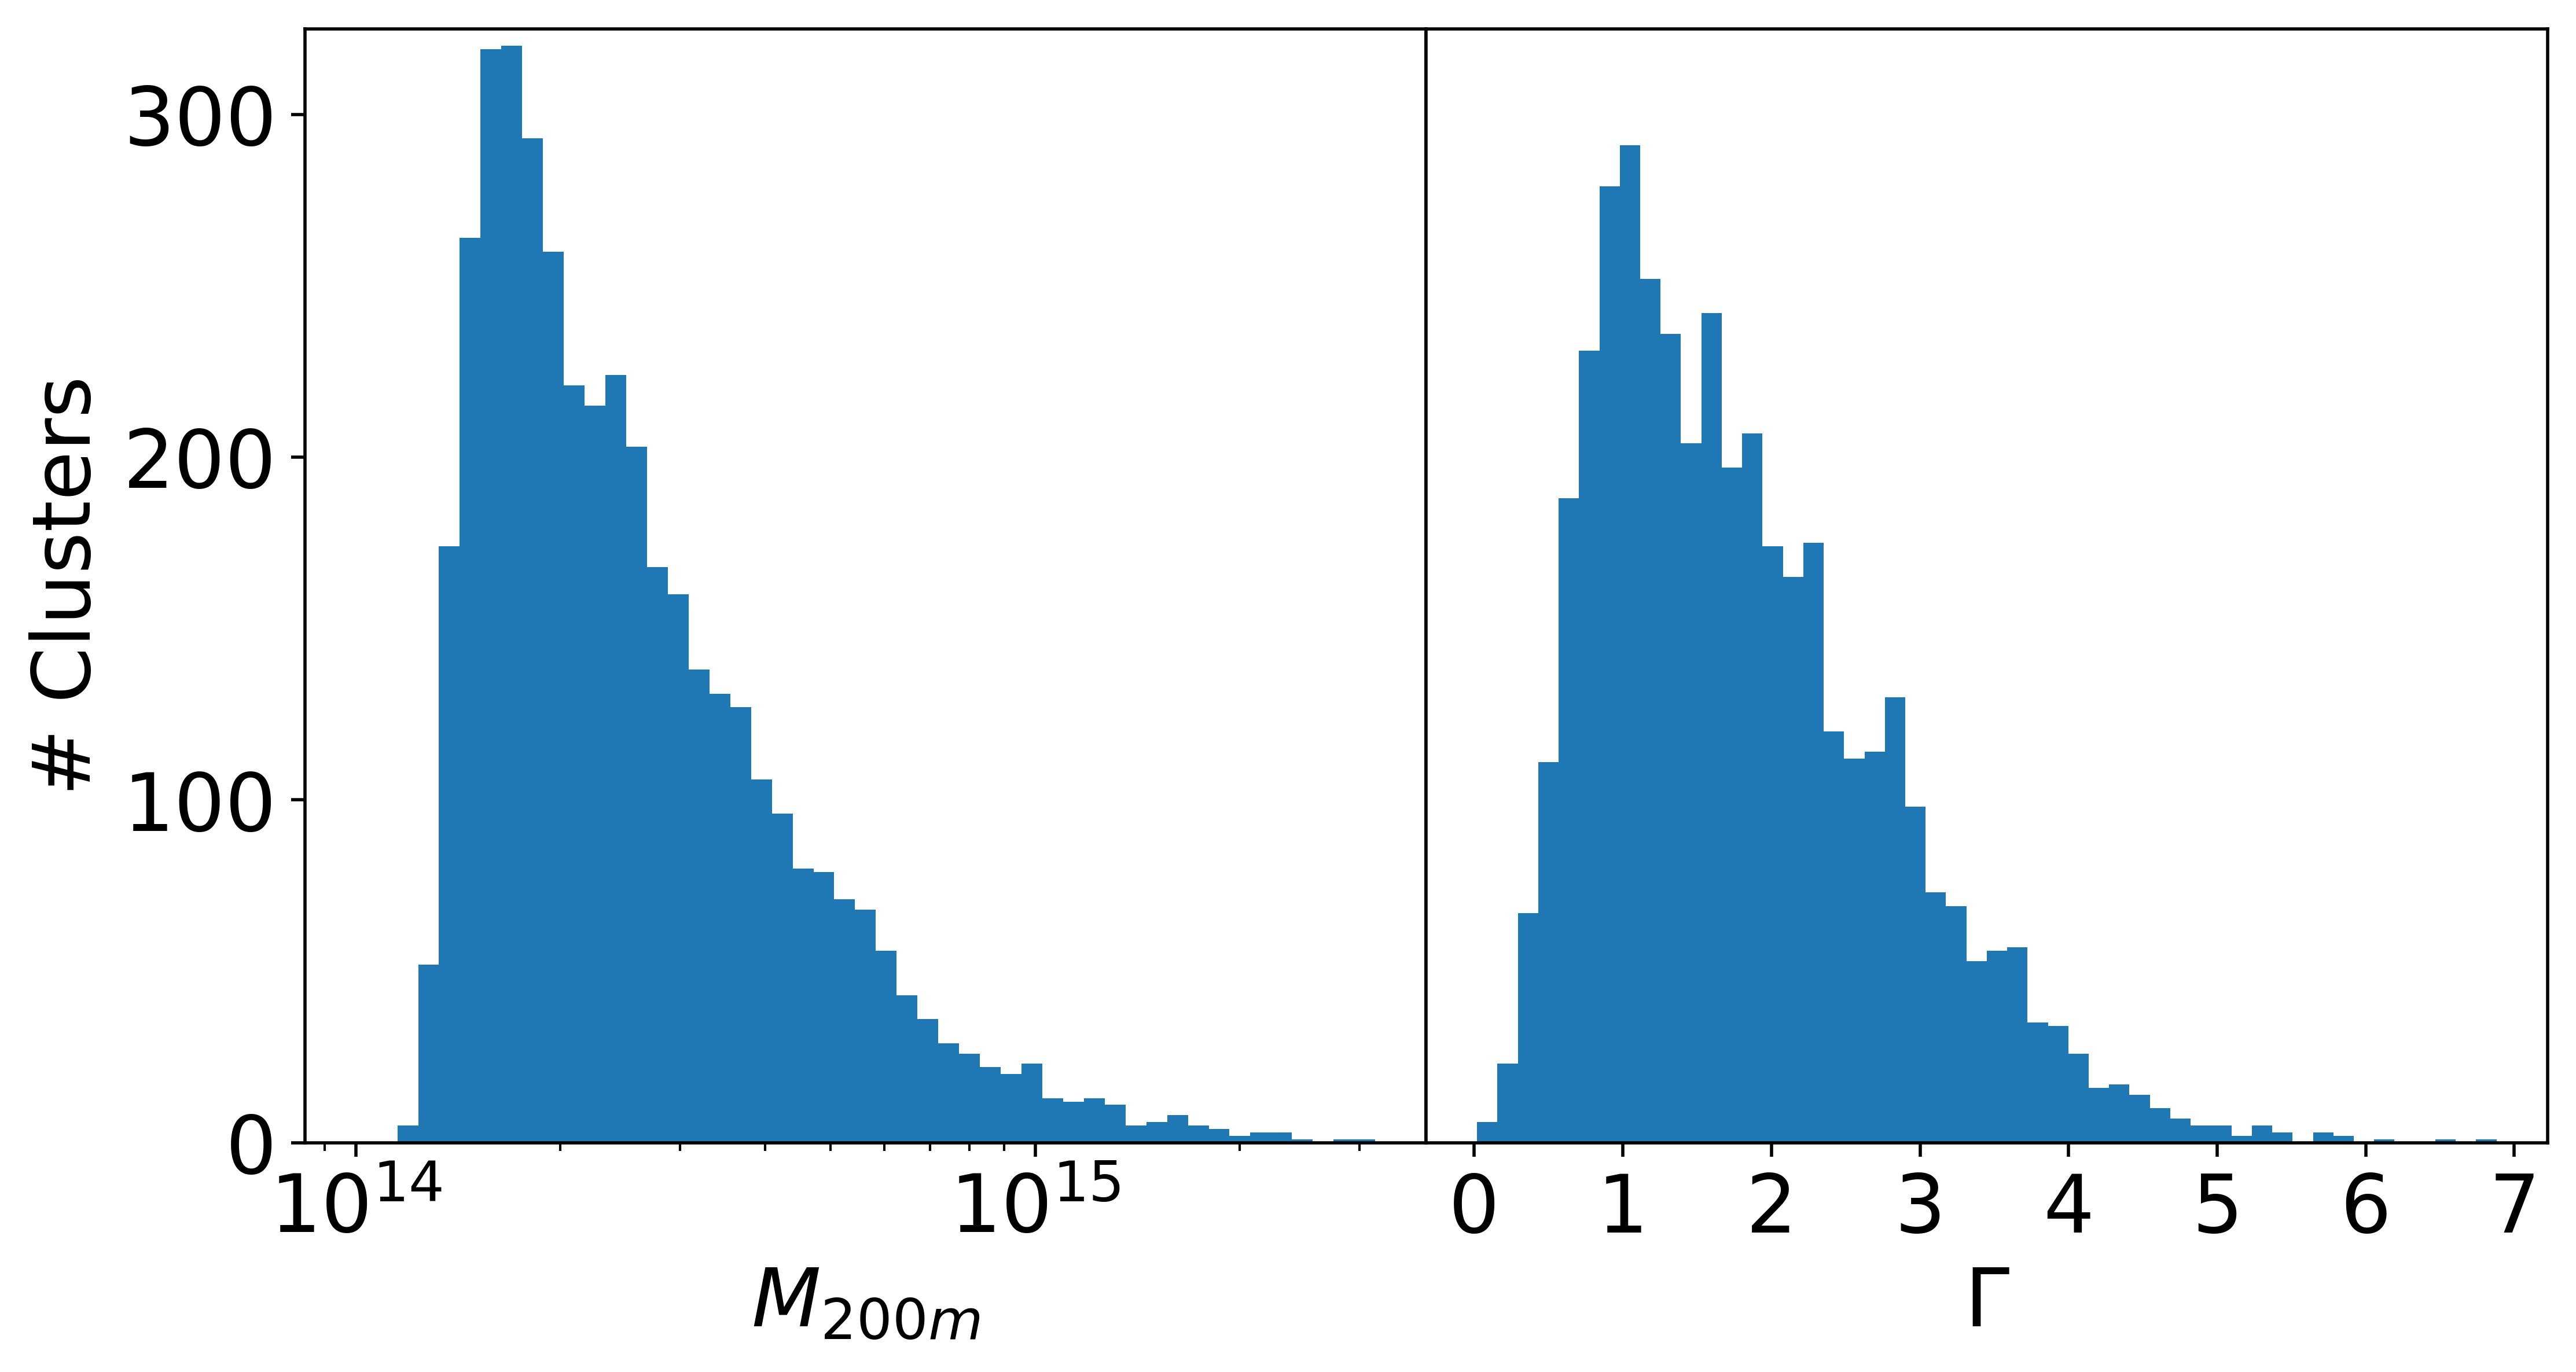
\includegraphics[width=\textwidth]{Ch4_MAH_Est/MAR_and_Mass_Dists.png}
    \caption{\raggedright Histogram of mass ($M_{200m}$) and MAR ($\Gamma$) values for the simulated galaxy clusters.  Both distributions are highly non-uniform.  To mitigate the biases that may be introduced by this non-uniformity, the MAR values are converted to z-score values for training. Further analyses of sources of bias is discussed in Section~\ref{Ch4_biases}.}
    \label{fig:data_dist}
\end{figure}


\begin{figure*}
    \centering
    %\null \vspace{-5pt}
    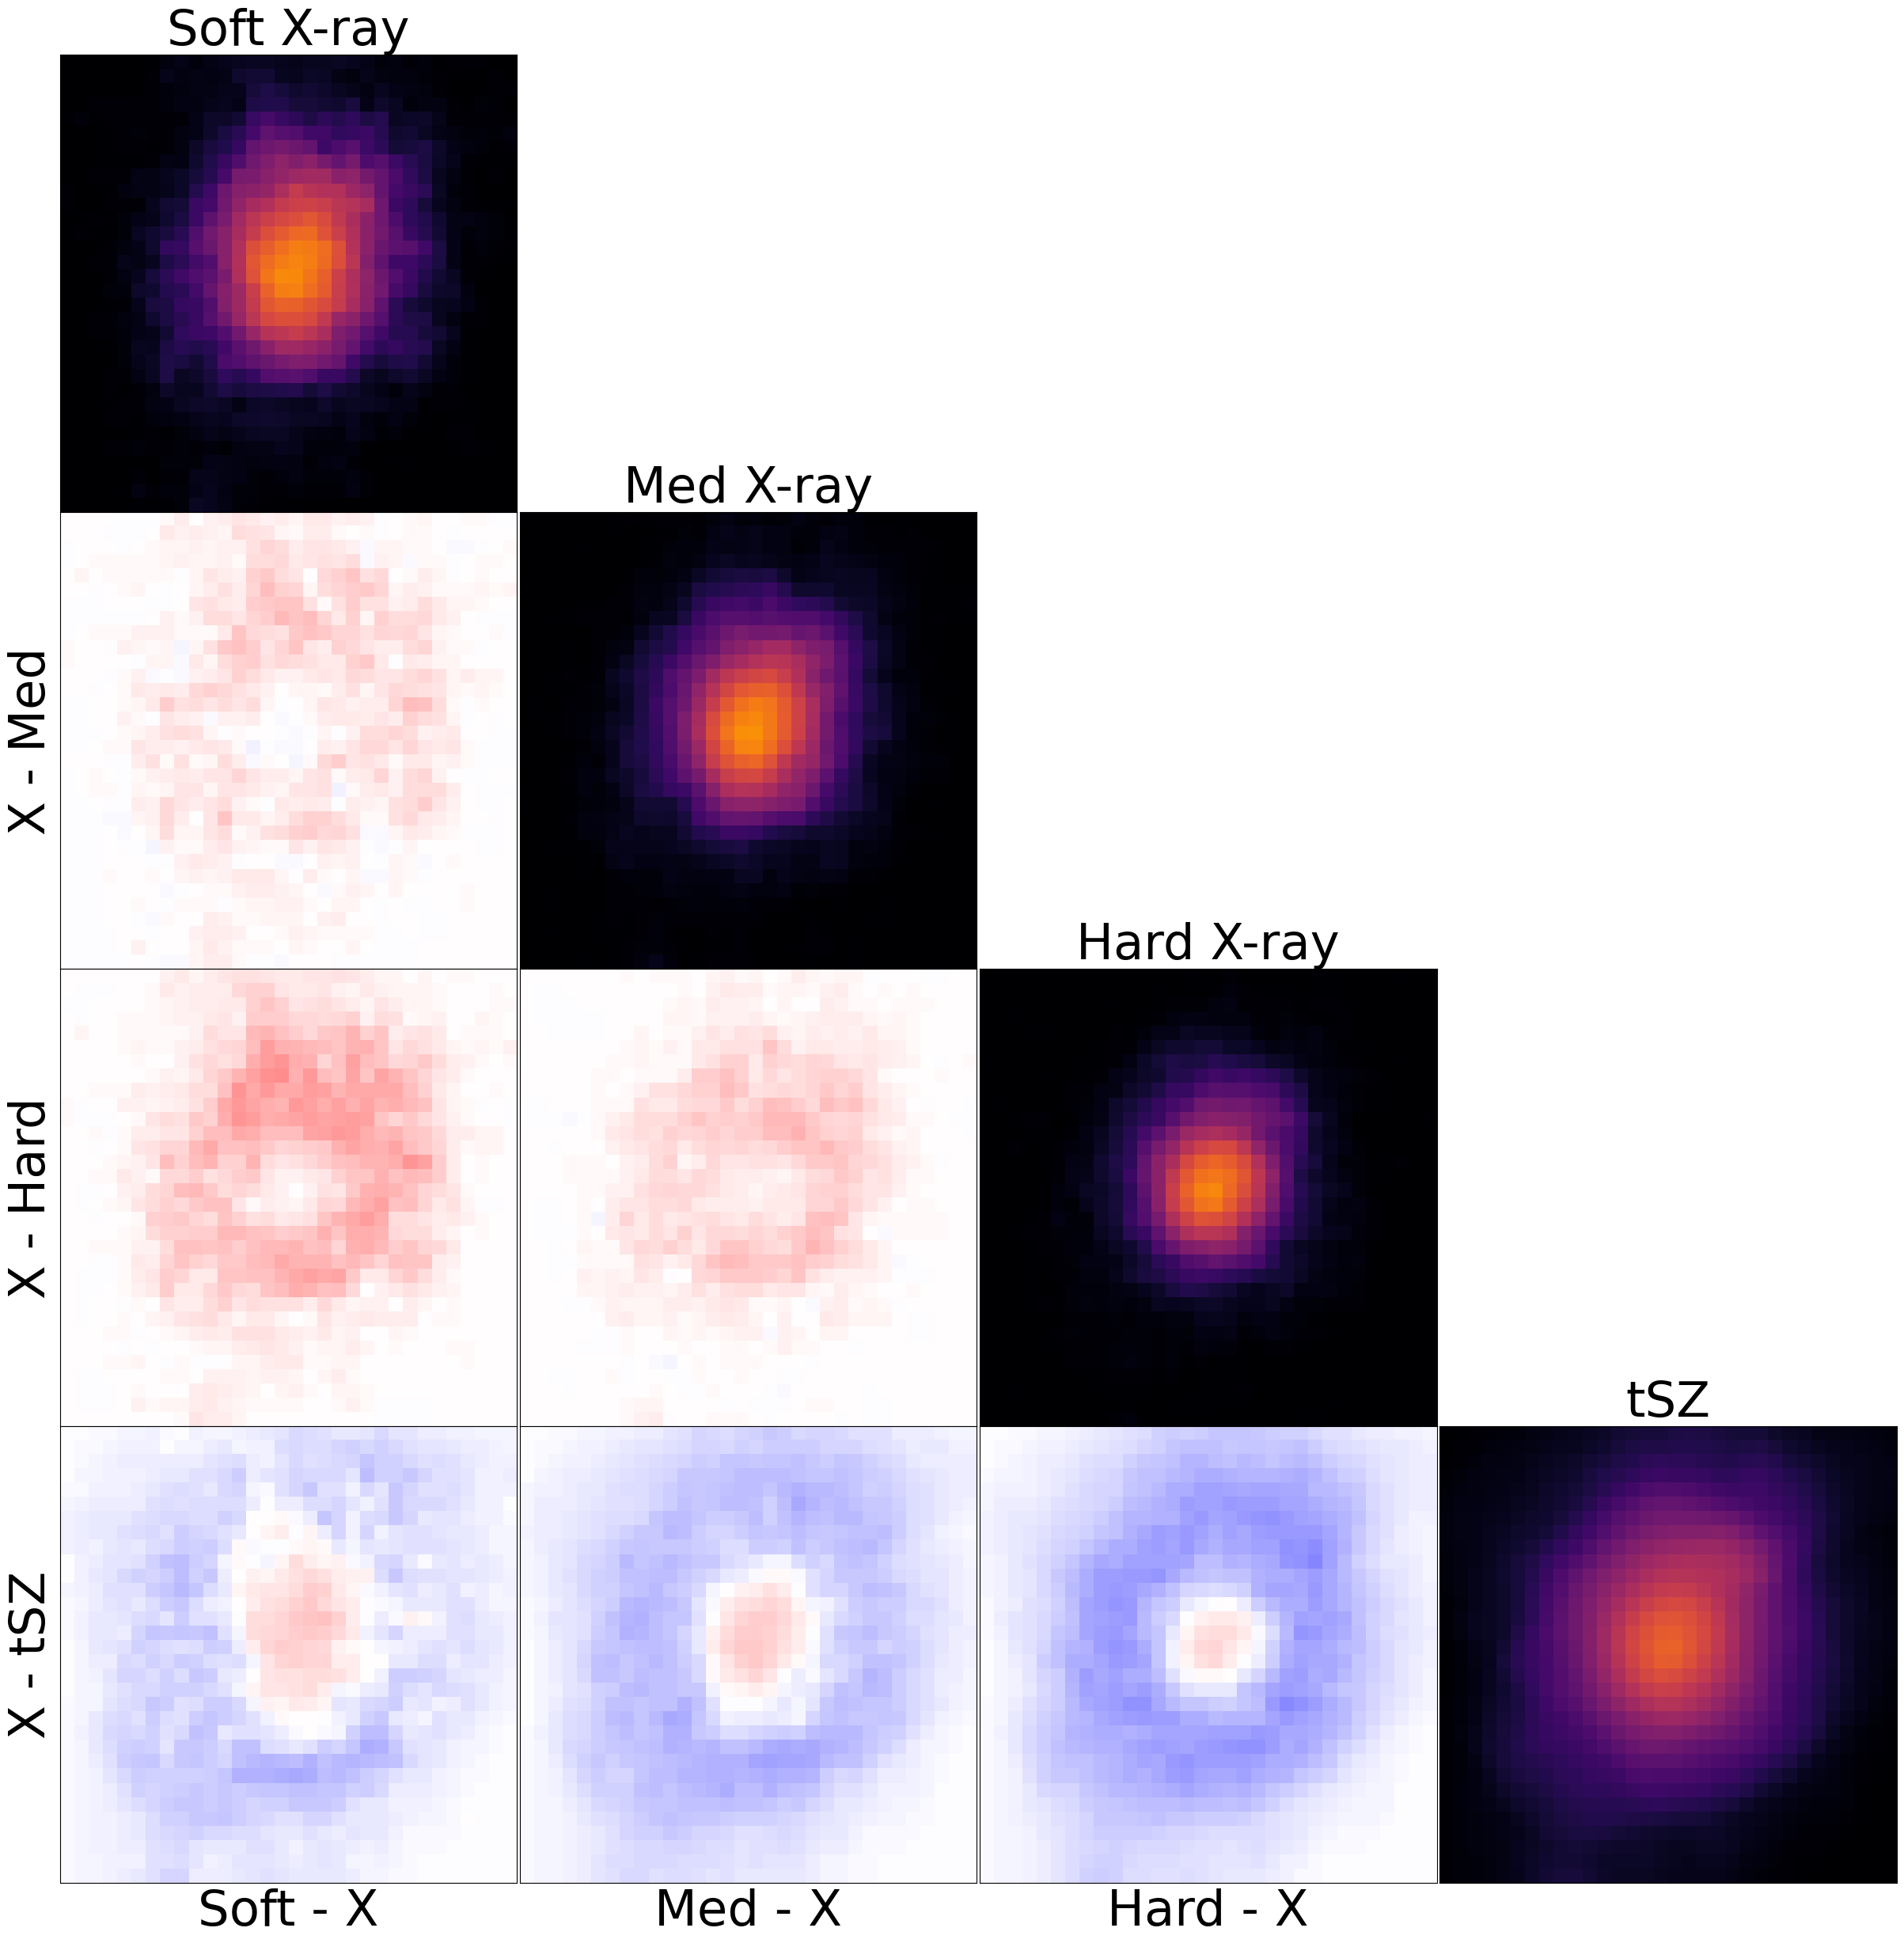
\includegraphics[width=\textwidth]{Ch4_MAH_Est/Image_Bands_091624_12177.png}
    \caption{\raggedright A representative galaxy cluster mock observation across several energy bands. Each image at the top of a column is derived from the MTNG simulation and has been artificially lowered to 32x32 pixel resolution and then normalized following equation \ref{eqn:norm}. X-ray images show photon count in the corresponding energy bin, while tSZ image shows the Compton-y value. This example cluster has a true mass of $M_{200m}=2.76\times10^{14}M_{\odot}$ and a MAR of $\Gamma = 1.79$; from the distribution of masses and MARs in Figure \ref{fig:data_dist}, we see that this is a ``typical'' cluster. We also show the subtractions of each image to illustrate the spectral information available to the model. For more details about the simulation and mock observations, see Section \ref{Ch4_data}. }
    \label{fig:sample_obs}
\end{figure*}

For each galaxy cluster, we calculate the MAR according to the definition of \cite{Diemer_2020},
\begin{equation}\label{eqn:MAR_def}
    \Gamma_{\mathrm{dyn}} = \frac{\Delta \log M_{200m}}{\Delta \log a} \,.
\end{equation}
The time interval is the dynamical time, which we take to be the crossing time of the cluster at radius $R_{200m}$, written in units of the change in the logarithm of the scale factor $a$. This definition of MAR has been shown to most closely correlate with the dynamical state of the halo, and thus its splashback radius \cite{Shin_2023}. For further discussion of the relation between our choice of MAR and other definitions, see also \cite{Valles_Perez_2020}. Algorithmically, we calculate MARs using the \textsc{HydroTools} code \cite{diemer_17_sfh, diemer_18_hih2}, which follows the most massive progenitor history of each halo as tracked by the Subfind-HBT halo finder \cite{Springel_2021}. When training our model, we normalize our MARs by subtracting the mean MAR and dividing by their standard deviation, constructing a $z$-score. This normalization reduces the range of values and centers the values at zero, which improves the accuracy of the model. The distributions of MARs and mass values in our dataset are shown in Figure \ref{fig:data_dist}. 

\subsection{ML Model}\label{Ch4_models}
Our model is a combination of a normalizing flows model \cite[see][for a review of normalizing flows]{Papamakarios_2019} and a convolutional neural network (CNN) model \cite[see][for a review of CNN and deep learning]{LeCun_2015}. We choose a CNN model to compress MAR-relevant information in the mock observations. We feed that information into the normalizing flows model, which allows us to perform posterior density estimation, giving us a measure of the uncertainty on the MAR estimate for each galaxy cluster. 

\begin{figure*}
    \centering
    %%\null \vspace{-5pt}
    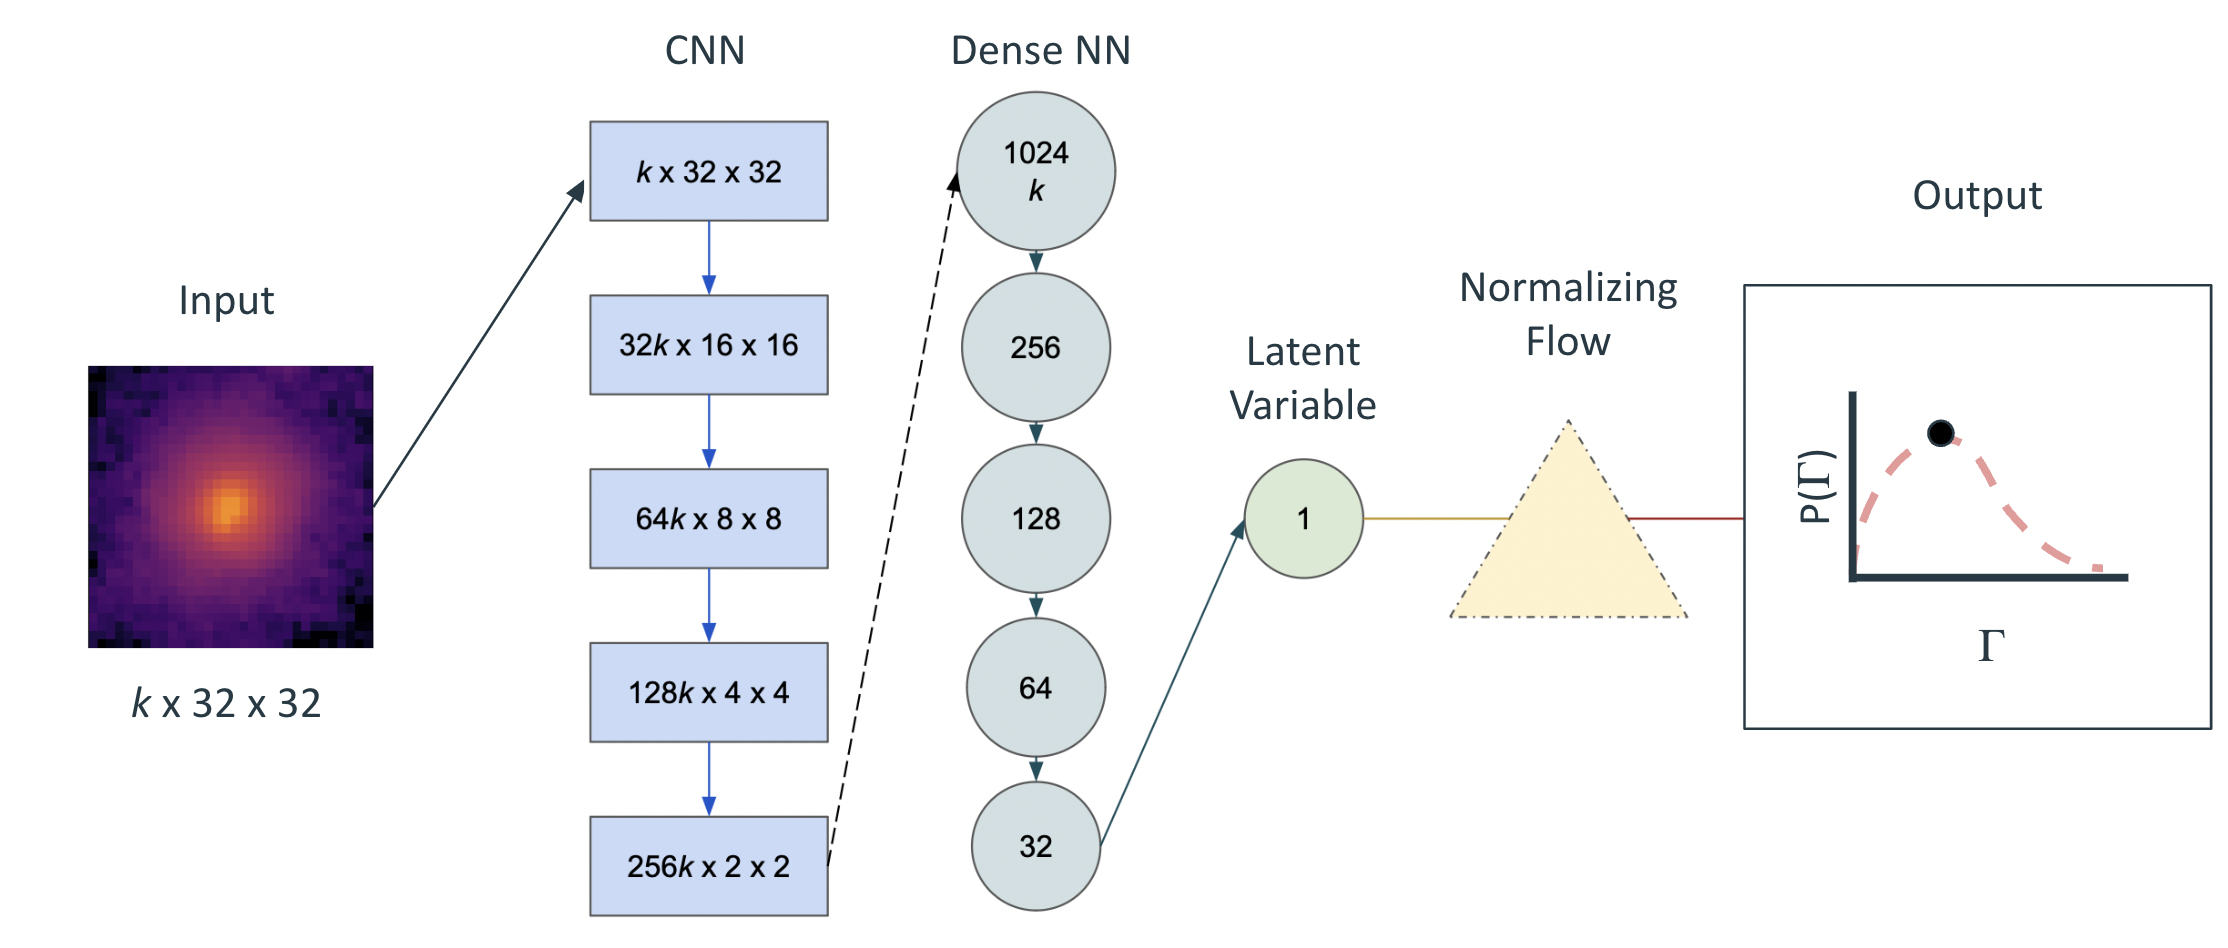
\includegraphics[width=\textwidth]{Ch4_MAH_Est/model_diagram_2.png}
    \caption{
    %\raggedright 
    A visualization of our ML model for an input with $k$ observation types. In the CNN portion of the model, images (blue boxes) are fed through a convolutional layer with a Leaky ReLU nonlinear activation function and a global pooling function (blue arrows). After four convolutional layers the final image is flattened out (black dashed arrow) into $1024 \times k$ weights. These are compressed through a series of fully connected layers (dark cyan arrows), each producing a smaller output (cyan circles). This culminates in a single latent space variable (green circle), which is then inputted into the normalizing flows model (yellow triangle) before outputting a sample MAR estimate from an approximation of the distribution of possible MARs given the input observation (far right).}
    \label{fig:model_diagram}
\end{figure*}

Our CNN model was written in the \texttt{Python} package \texttt{Pytorch}\footnote{\url{https://pytorch.org/}} and our normalizing flows model and training were implemented in the \texttt{Python} package \texttt{SBI}\footnote{\url{https://sbi-dev.github.io/sbi/}}. The CNN model serves as an embedding network, compressing the $4\times32\times32$ dimensional observation data into a single latent space variable. It does so utilizing convolution layers, which exploit locality and the translational invariance of features to efficiently compress information in images to higher levels of abstraction. 

Our CNN model consists of four convolution layers, the first starting with $32\times n_{\mathrm{obs}}$ filters, where $n_{\mathrm{obs}}$ is the number of observation types used (e.g., Soft X-ray only, or Soft X-ray and tSZ). Each subsequent convolution layer has twice as many filters as the previous layer. After each convolution layer, we apply a leaky ReLU layer \cite{LeakyReLU_2015} (unlike a standard ReLU, the $<0$ half has a non-zero slope) and then a two-dimensional max pooling layer, which reduces the dimensions of the image by a factor of two. At the end of the convolution layers, we are left with $256\times n_{\mathrm{obs}}$ images that are $2\times2$ pixels. We flatten this into a one-dimensional array, and four dense node layers follow. The first layer has $256\times n_{\mathrm{obs}}$ weights, and each subsequent dense layer has half as many. Between each layer, we once again apply a leaky ReLU non-linear activation function. After these dense layers, we apply one final dense layer, again with a leaky ReLU activation function, producing a single-scalar output, which we refer to as our latent space variable. The latent space variable is then inputted into the normalizing flows model. A diagram of our CNN model is shown in Figure \ref{fig:model_diagram}. It is possible that a different CNN model architecture could improve performance. While we did not aim to optimize our hyperparameters, we did explore a variety of possible model parameters, including increasing or decreasing the number of weights, changing the number of latent space variables that the CNN outputs, and removing max-pooling layers. We find that these changes did not improve model performance. The goal of our work is to demonstrate that such a model is possible and useful, not to provide a model ready for use on real data (see Section \ref{Ch4_conclusion} for a further discussion concerning this point). 

The normalizing flows model trains a set of invertible transformations that map the data distribution (possible MARs of a cluster) to a base distribution (e.g., a normal distribution). By reversing these transformations, one can easily sample the base distribution, and thereby attain samples of the data distribution. A more detailed description of the exact procedure used to train our normalizing flows variant can be found in \cite{Greenberg_2019}. Our normalizing flows model, a SNPE-C type model \cite[][see also the \texttt{SBI} documentation]{Papamakarios_2018, Greenberg_2019}, uses the default model settings of the \texttt{SBI} package. We experimented with increasing the number of weights and transforms by a factor of two or more but found no significant improvement and increased computational demand. A diagram of our full model is shown in Figure \ref{fig:model_diagram}. 

\subsection{Fitting Function}\label{Diemer_2020}
To assess the effectiveness of our model, we compare its performance to the MAR fitting function of \cite{Diemer_2020}, which approximates MAR as defined in Equation \ref{eqn:MAR_def} as a function of mass and redshift,
\begin{equation}\label{eqn:Diemer_2020}
    \Gamma  = A\nu + B\nu^{3/2}
\end{equation}
\begin{equation}\label{eqn:Diemer_2020_A}
    A = 1.1721 + 0.3255z
\end{equation}
\begin{equation}\label{eqn:Diemer_2020_B}
    B  = -0.2565 + 0.0932z - 0.0571z^2 + 0.0042z^3 \,.
\end{equation}
Here, mass is expressed as peak height, $\nu$, which is a function of the $M_{200m}$, redshift, and cosmological parameters. $A$ and $B$ encode the redshift dependence through simple polynomial fits. We calculate the peak heights of each cluster using the \textsc{Colossus} code \cite{Diemer_2018} and use the transfer function from \cite{Eisenstein_1998} to approximate the power spectrum. The best-fit parameters of the fitting function are based on data from the Erebos suite of $N$-body simulations, which contains two different $\Lambda$CDM cosmologies \cite{Diemer_2020}. 

Since our galaxy clusters are all from a single cosmology and a single redshift, the fitting function is only a function of mass (see Figure \ref{fig:diemer_v_mass}). The fitting function could be biased for a number of reasons including biases introduced by training on an $N$-body simulation and applying to a simulation with baryonic physics and biases from specific non-physical artifacts in the $N$-body code \cite[for a discussion of the robustness of MARs in $N$-body simulations see][]{Soltis_2024}. More importantly, the intrinsic scatter in MARs about any given galaxy cluster mass is high. The combination of these factors, but mostly the latter factor, means that the estimates of the fitting function are only weakly correlated to true MARs. A simple analysis reveals that the Pearson correlation coefficient \cite{Pearson_1895} between the estimates of the fitting function and the true MAR is $0.19$, while our ML model has a correlation coefficient of $0.77$ (for a more detailed discussion of the accuracy of the models, see Section \ref{Ch4_results}).

\begin{figure}%[b]
    \centering
    %\null \vspace{-5pt}
    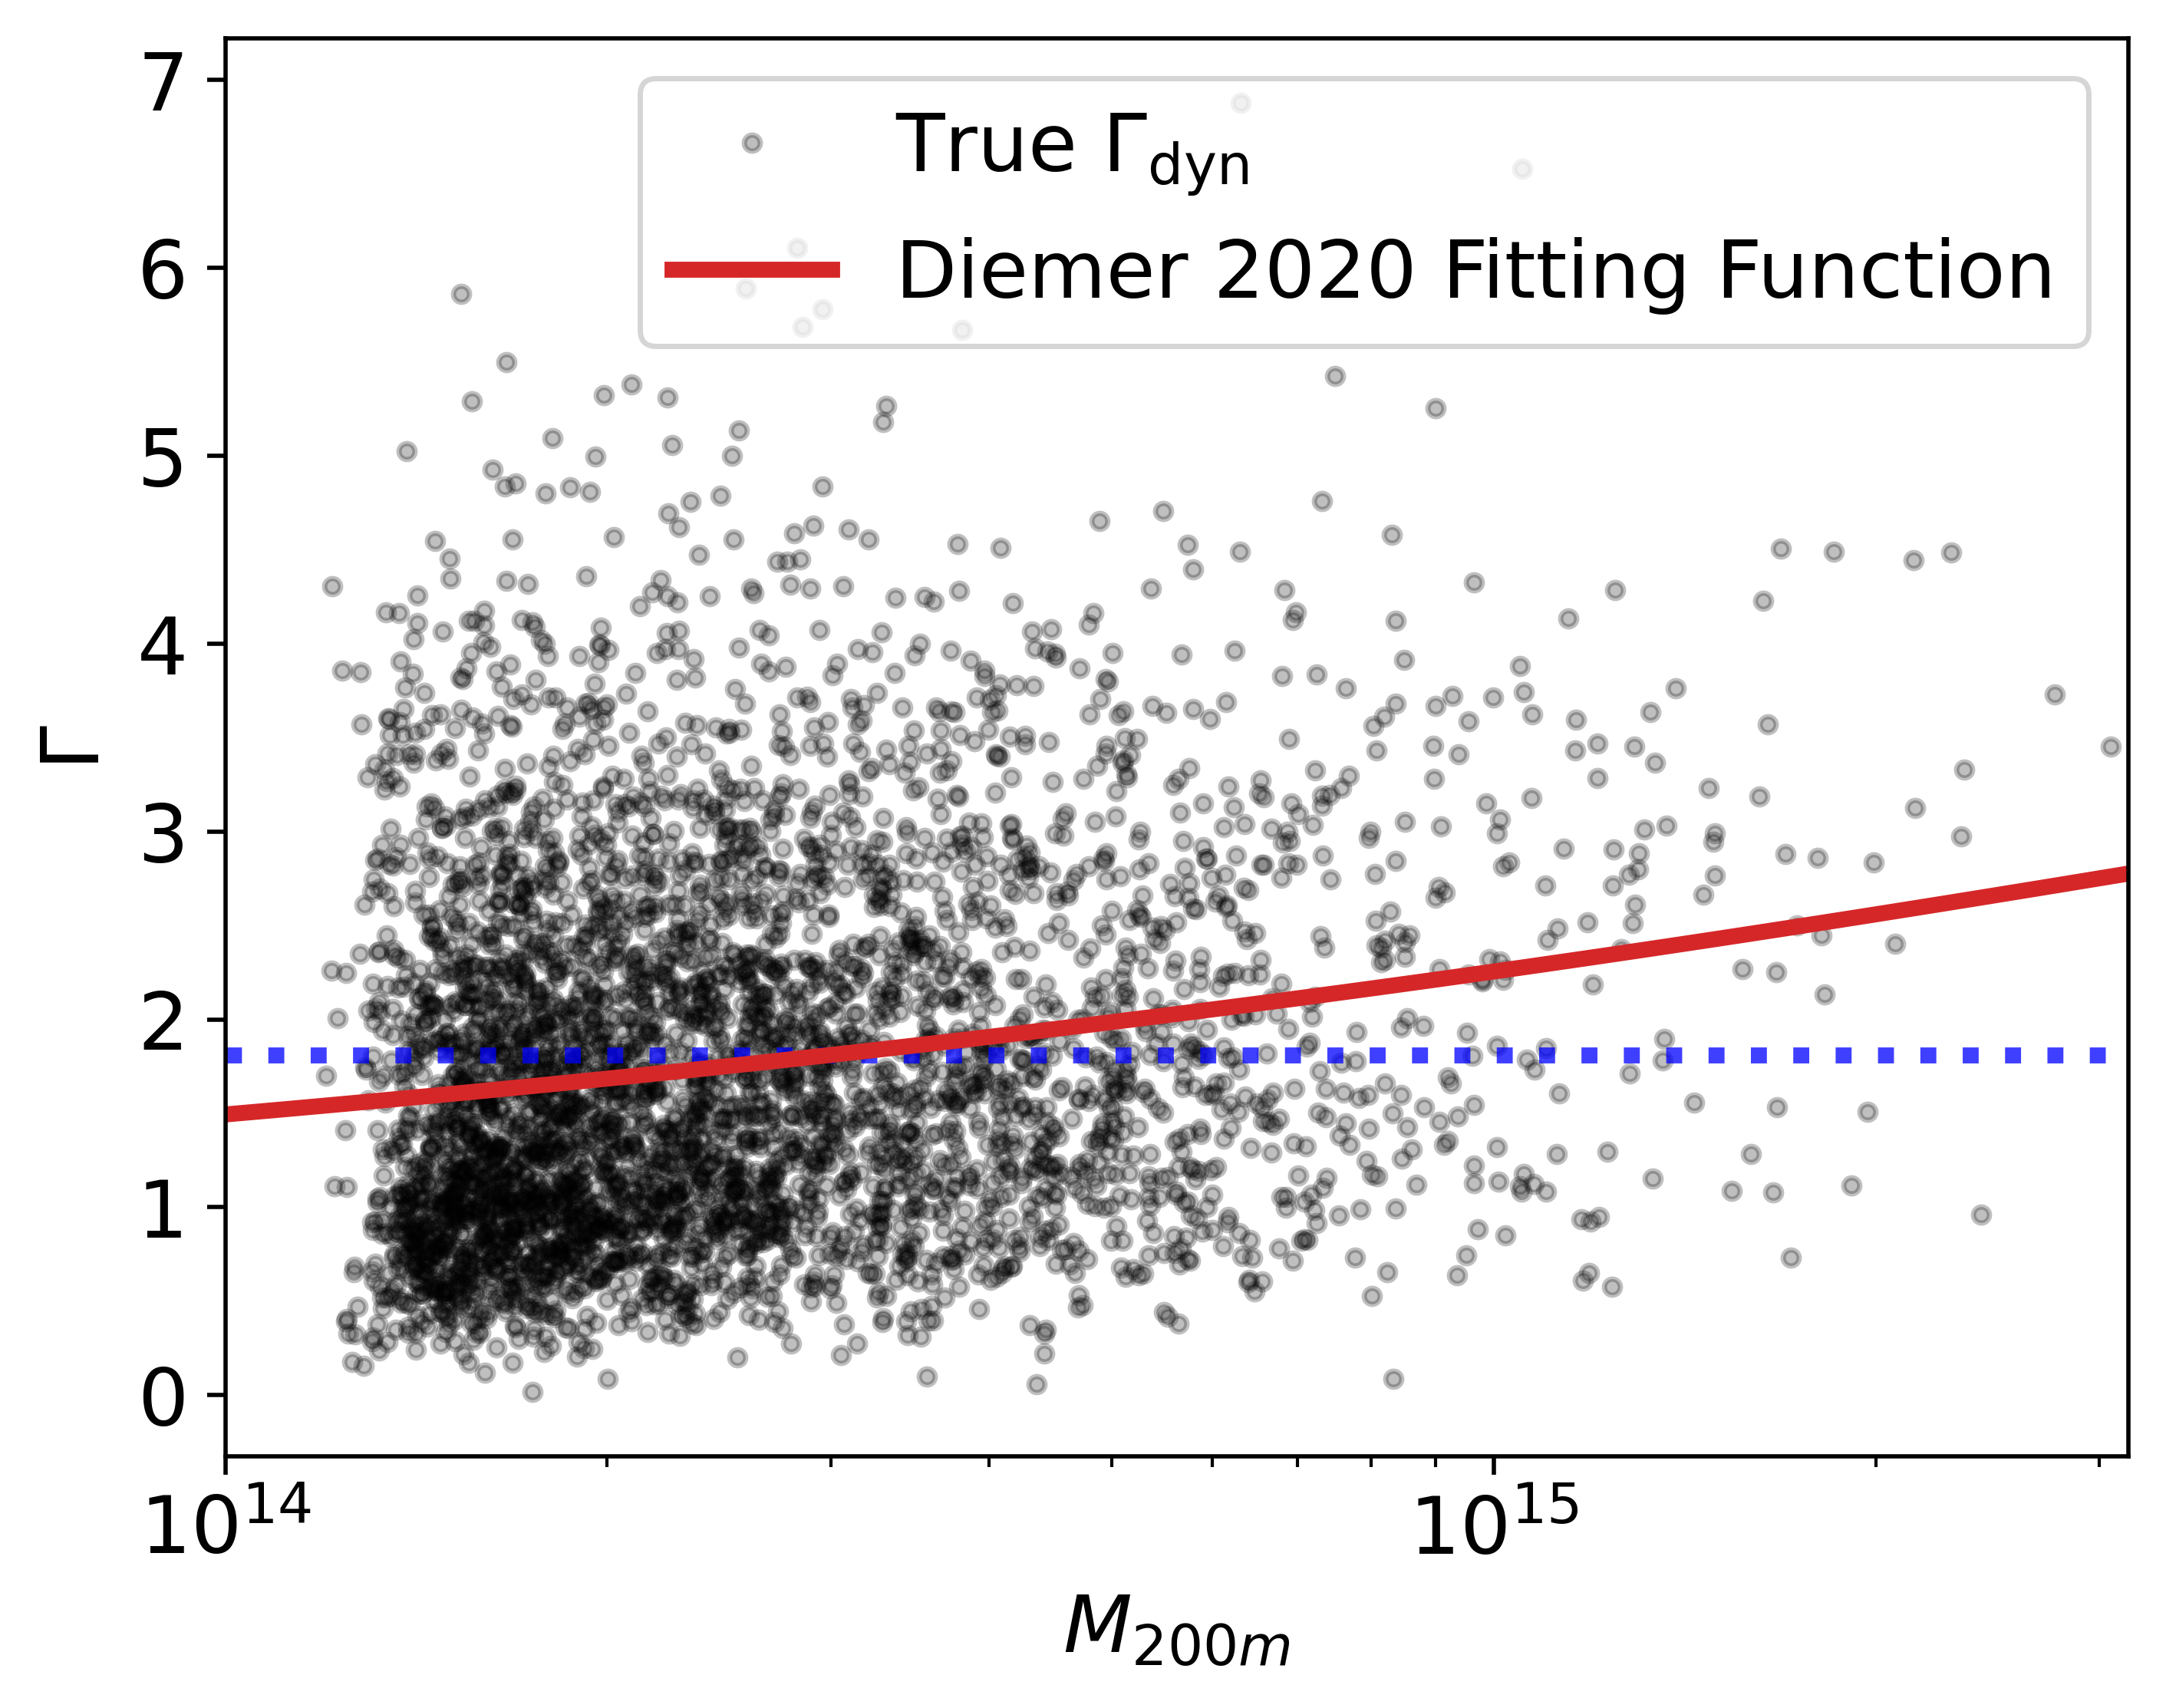
\includegraphics[width=\textwidth]{Ch4_MAH_Est/Diemer_2020_vs_M200m_091424.png}
    \caption{\raggedright A comparison of the fitting function to the true MAR for MTNG clusters in the dataset. The fitting function (red line), taken from \cite{Diemer_2020}, is a poor fit for the true MARs (black dots) of the MTNG galaxy clusters. For a fixed cosmology and redshift, the fitting function is solely a function of the galaxy cluster mass, which is weakly predictive of the MAR. Even so, the fitting function is the best existing non-ML method for estimating $\Gamma_{\mathrm{dyn}}$. The mean $\Gamma_{\mathrm{dyn}}$ (blue dotted line) is shown for comparison.}
    \label{fig:diemer_v_mass}
\end{figure}

\subsection{Training}\label{Ch4_training}
The data is divided into tenths so that a 10-fold validation could be performed. Each tenth of data are assigned to a different test set, with the remaining data put in the validation and training set. Each fold contained a unique set of clusters, meaning that different lines of sight of the same cluster and rotations of a cluster observation were kept within the same data fold. The model training was handled by the \texttt{SBI} package\footnote{\url{https://sbi-dev.github.io/sbi/latest/reference/\#sbi.inference.snpe.snpe\_c.SNPE\_C.train}}. A batch size of 32 images was used. The default training function parameters were used. Model training automatically stopped when the validation loss failed to improve after 20 epochs. The typical training lasted $\sim30$ epochs. When analyzing our model's performance, we apply each model to its unique test set and then examine the joint set of estimates produced by all models.

In addition to training our model on all four possible observations of a given galaxy cluster (Soft X-ray, Medium X-ray, Hard X-ray, and tSZ), we also train to other variants on subsets of that data. The X-ray-only model is trained only on the X-ray observations of the clusters, and the tSZ-only model is trained only on the tSZ observations of the data. All other aspects of the training procedure and analysis are the same.

\section{Results}\label{Ch4_results}
The principle advantage of using a normalizing flows model in our work is its capacity to estimate the posterior density, that is, the probability of the cluster having a given MAR given the observations of the cluster. We can then use this information to provide an estimate of the MAR and uncertainties for that estimate. For computational reasons, we approximate this procedure using 1000 samples from the trained machine-learning model. The median MAR estimate of the sample set is chosen as the fiducial estimate, and the 16th and 84th percentiles of the sample set are given as uncertainties. In the following subsections, we present the results of our model. In Section~\ref{Ch4_accuracy}, we analyze the accuracy of the fiducial estimate and compare it to a fitting function. In Section~\ref{Ch4_uncertainty}, we examine the accuracy of our uncertainty estimates. In Section~\ref{Ch4_biases}, we test our fiducial estimate for biases. Finally, in Section~\ref{Ch4_data_robustness}, we explore variants in the training data and model and what impact those choices have on model performance.

\subsection{Mass Accretion Rate Estimates}\label{Ch4_accuracy}
To evaluate the overall accuracy of our ML model, we compare the accuracy of its estimates as compared to the accuracy of the fitting function. We do so by generating 1000 sample estimates for each cluster observation in the test set of each model, calculating the median of each sample set, and comparing that to the true MAR of the cluster, as determined using the procedure described in Section~\ref{Ch4_data}. To make these results more interpretable, we convert the errors from units of MAR to percent error.

The resulting error distributions for the entire dataset are shown in Figure \ref{fig:percent_error}. Examining the absolute error, we find that our ML model outperforms the fitting function by nearly a factor of two. Moreover, we find that the use of a subset of the available observation modes does not substantially reduce the accuracy of the estimates. These results demonstrate that our dataset is sufficiently large to learn useful information for estimating the MAR. Even so, a larger training set would likely lead to greater accuracy. A tabular breakdown of our results is found in Table \ref{tab:median_est_errors}.

\begin{table*}[]
    \centering
    \begin{tabular}{|c | c c c|} 
    \hline
    \textbf{MAR Estimator} & \textbf{50\%} & \textbf{68\%} & \textbf{95\%} \\
     & & & \\
    \hline
    \hline
    Fitting Function & 39\% & 56\% & 203\% \\ 
    \hline
    X-ray \& tSZ ML Model & 22\% & 33\% & 88\% \\
    \hline
    X-ray ML Model & 23\% & 35\% & 98\% \\
    \hline
    tSZ ML Model & 23\% & 34\% & 90\% \\
    \hline
    \end{tabular}
    \caption{The error of each estimator, for a given percent of the dataset. For example, for the MAR estimates produced by the fitting function, 50\% of the clusters in our dataset have a percent error of 39\% or less. The results show that the ML model out performs the fitting function by nearly a factor of two. Moreover, using either the X-ray observations alone, or the tSZ observations alone, does not result in a substantial loss of accuracy.}
    \label{tab:median_est_errors}
\end{table*}

\begin{figure*}
    \centering
    %\null \vspace{-5pt}
    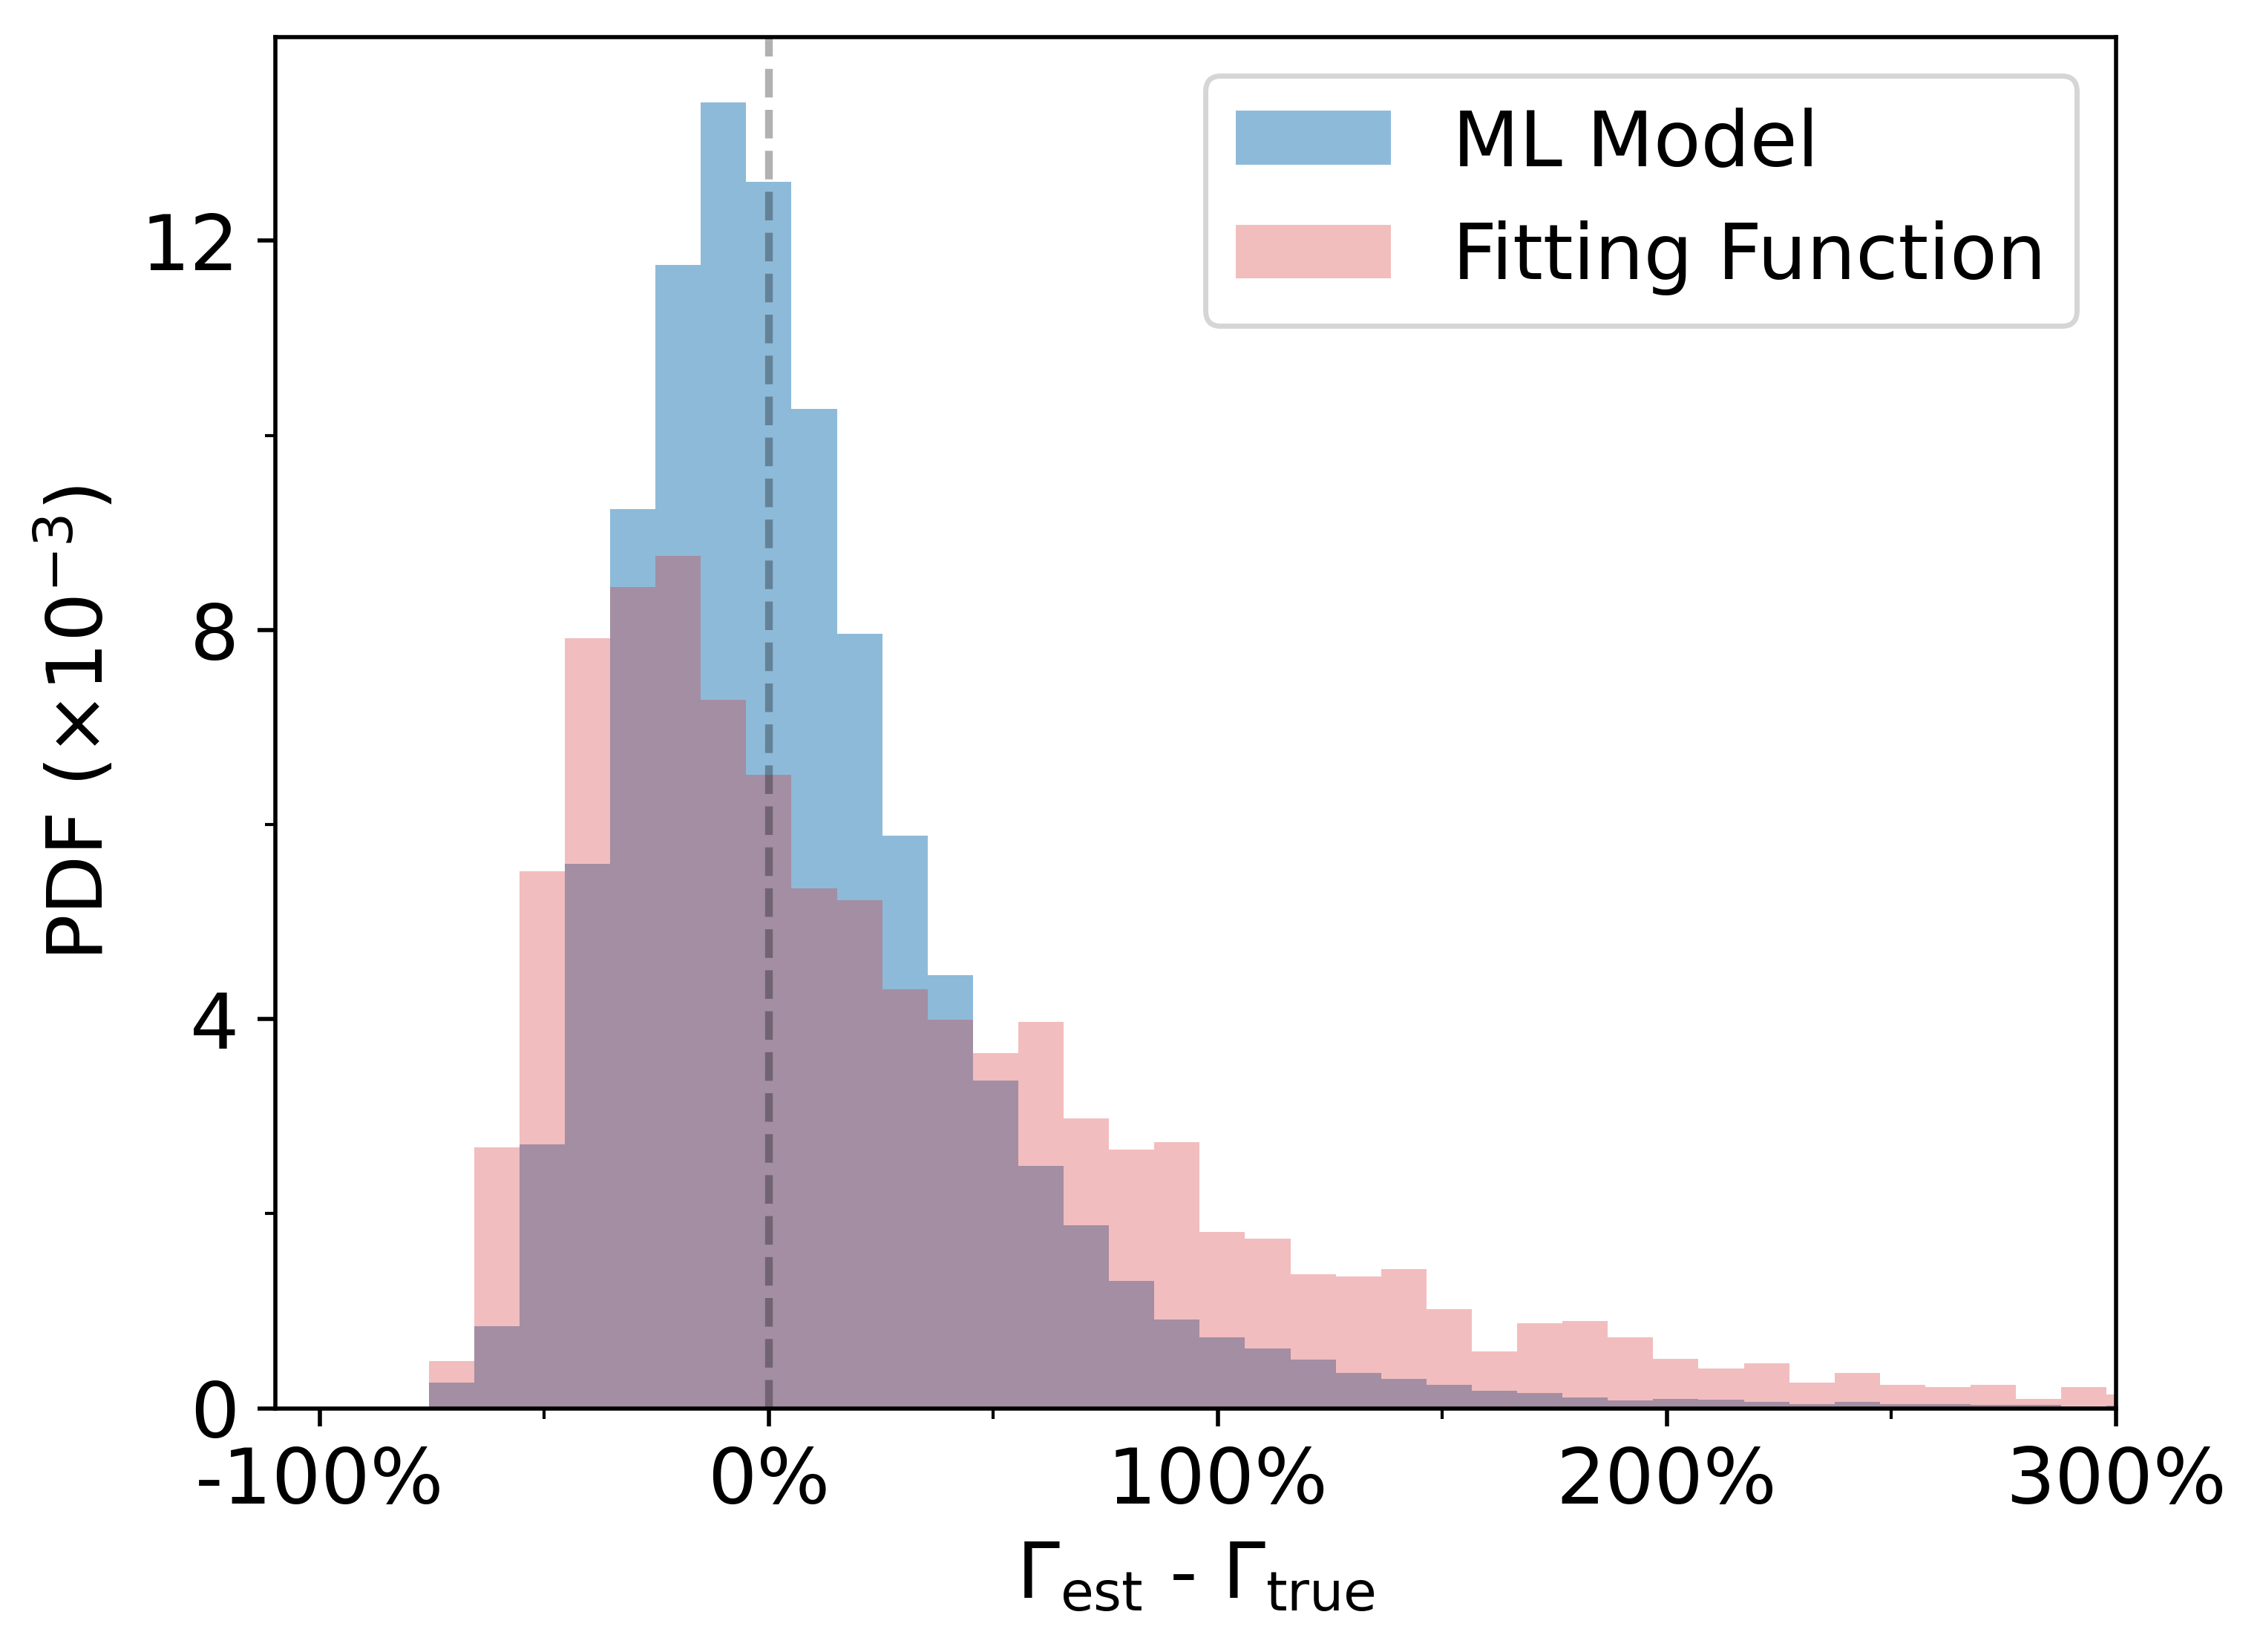
\includegraphics[width=\textwidth]{Ch4_MAH_Est/Prediction_Percent_Error_Hists_NF_CNN_SPM_MW_All_Masses_tanh_rotations_all_folds_091624.png}
    \caption{\raggedright Histogram of the percent error of the ML model MAR estimates (blue) compared to the fitting function (red). The ML model's error distribution has a smaller tail than the fitting function. For the ML model only 4\% of the cluster observations tested have MAR estimates with percent errors greater than 100\%. For the fitting function, this jumps to 16\% of the cluster observations tested. Similarly, more than half (56\%) of the observations tested have ML model estimates with less than 25\% error, but this reduces by a factor of 2 (33\%) for MAR estimates produced by the fitting function. A description of how the error is calculated can be found in Section~\ref{Ch4_accuracy}.}
    \label{fig:percent_error}
\end{figure*}

\subsection{Uncertainties}\label{Ch4_uncertainty}
How accurate are the uncertainty estimates produced by the model? We test this by examining how closely the model-generated confidence intervals match expectations. First, a single set of observations, we calculate the model-provided confidence interval using percentiles from the 1000 MAR estimate sample (see the introduction of Section \ref{Ch4_results}). Second, we calculate whether the true MAR is contained within a given confidence interval (as calculated using the aforementioned percentiles). We repeat this procedure for the entire test set and for different potential confidence intervals. A visualization of the results is shown in Figure \ref{fig:uncertainties}. We find that the observed confidence interval, i.e., the frequency at which the true MAR is between the sample-derived percentiles, is a 1-5\% underestimate of the true uncertainty. We also find that using only X-ray or tSZ observations does not strongly impact the accuracy of the uncertainty estimates. We perform this evaluation over all fold-unique models (see Section \ref{Ch4_training}), and find the variance in the observed confidence intervals ranges from 1-5\%. We repeated this analysis further by creating 10 more 10-fold divisions of the data, thereby training 100 new models in total. In evaluation of these new models, we found that the variance in the observed confidence intervals increased slightly, to a range $\sim$ 1-7\%. The worst underestimation in the model set underestimated the 50\% confidence interval by $11\%$. The most accurate observed confidence intervals were all within a percent of the ideal.

\begin{figure*}
    \centering
    %\null \vspace{-5pt}
    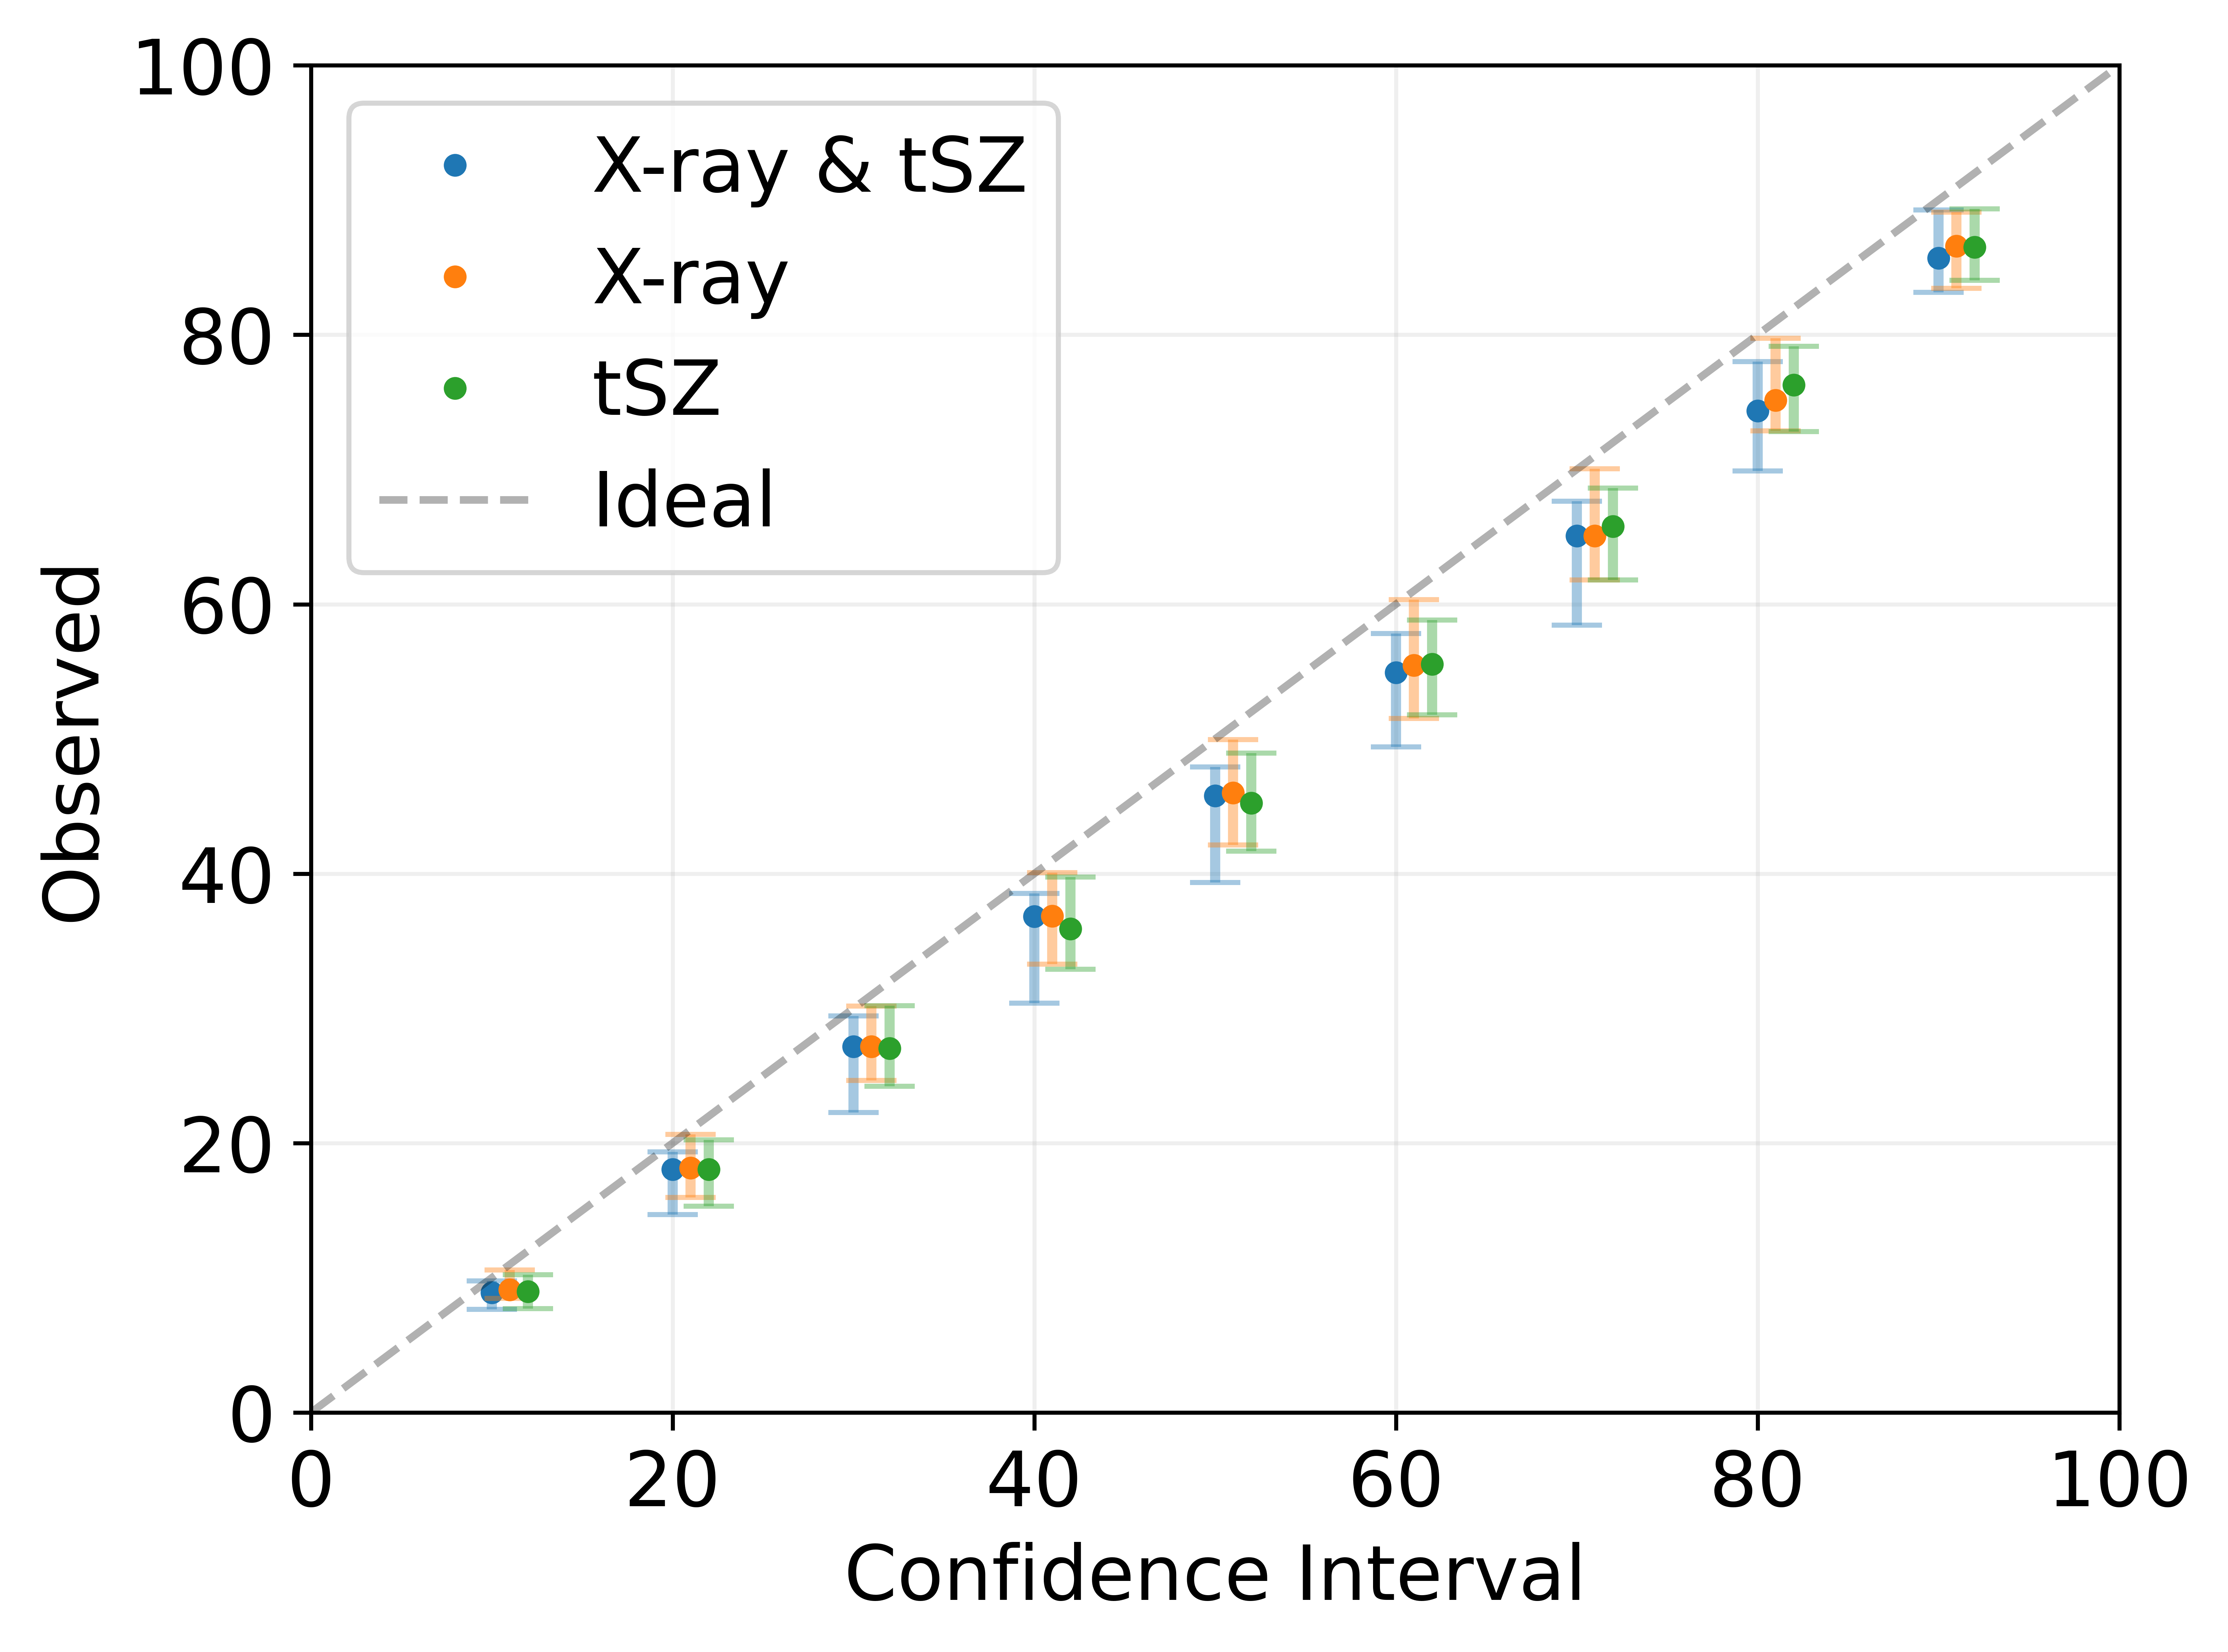
\includegraphics[width=\textwidth]{Ch4_MAH_Est/uncertainty_measurement_MW_Xray_tSZ_model_091624.png}
    \caption{\raggedright Representation of the accuracy of the uncertainty estimates provided by the ML model. The model provides an accurate measure of the MAR estimate uncertainty. The median observed confidence intervals (points) are near to the case of perfectly calculated uncertainties (dashed line) for all models. The best-performing fold-unique model (top line of error bar) typically sits on the idealized line. We repeated this analysis ten times, using different data splits, and found the results were qualitatively similar. The error on the uncertainty estimates for all model variants are comparable. See Section \ref{Ch4_uncertainty} for a detailed explanation of how the uncertainty estimate error is calculated. }
    \label{fig:uncertainties}
\end{figure*}

\subsection{Biases}\label{Ch4_biases}
ML models are excellent with interpolation, but can struggle with extrapolation. As discussed in Section~\ref{Ch4_data} and demonstrated in Figure \ref{fig:data_dist}, the mass and MAR distribution of the dataset is very non-uniform. From this information alone, we can suspect that the model is going to struggle to accurately estimate the MAR of clusters in the tails of the MAR distribution. If mass information is important for determining the MAR, it is also possible that the model will struggle with very low or very high mass clusters. 

In order to test for these biases, we examined our ML model's median MAR estimate error as a function of mass and MAR. To investigate a potential mass dependency in our MAR estimate errors, we separate our data into 12 evenly populated bins, each monotonically increasing in mass. We then calculate the median error of each bin as well as the 16th and 84th percentile errors. We find that the median error in the bin and the scatter in the bin are consistent across mass steps. This result holds for the X-ray-only and tSZ-only models as well. For comparison, when this procedure is performed on the fitting function, we find that low mass ($\leq2.5\times 10^{14} M_{\odot}$) clusters and high mass ($\geq 5\times10^{14}$) clusters are more likely to have their MAR overestimated (see the right plot of Figure \ref{fig:mass_mar_bias}). The difference between the ML model and the performance of the fitting functions demonstrates that the ML model uses more than just the mass information to constrain the MAR.

To investigate a potential MAR-dependent bias, we perform a similar binning analysis using the true MAR values of the clusters. We find evidence of a bias in the model's MAR estimates, with low MAR clusters ($\Gamma<1$) having overestimated MARs and ($\Gamma>2$) having underestimated MARs. These biases reflect the unbalanced nature of the distribution of true MAR in the dataset (see Figure \ref{fig:data_dist}). There is a long, narrow tail of very high MAR clusters in the distribution. The ML model is therefore underexposed to this region of parameter space and less effective at estimating these MARs. The signal-to-noise ratio of each cluster is uncorrelated with MAR, and therefore is not likely to be the source of this bias. Nevertheless, even here, the model still outperforms the fitting function, which struggles to accurately estimate high MARs. It is worth noting that tracking progenitors along merger trees can sometimes lead to discontinuities in the mass history, occasionally leading to erroneously extreme MAR \cite[][see discussion in section 6]{halo_finder_comp}. While SUBFIND-HBT seeks to minimize this, it is possible some of the extreme MAR in our dataset are non-physical, which may hinder the model's accuracy. Finally, we again find that the behavior of the X-ray-only and tSZ-only models mirrors the X-ray and tSZ model, except that the X-ray and tSZ model tends to have smaller errors, and therefore smaller biases. The results of this and the mass dependence analysis are shown in Figure \ref{fig:mass_mar_bias}.

\begin{figure*}%[b]
    \centering
    %\null \vspace{-5pt}
    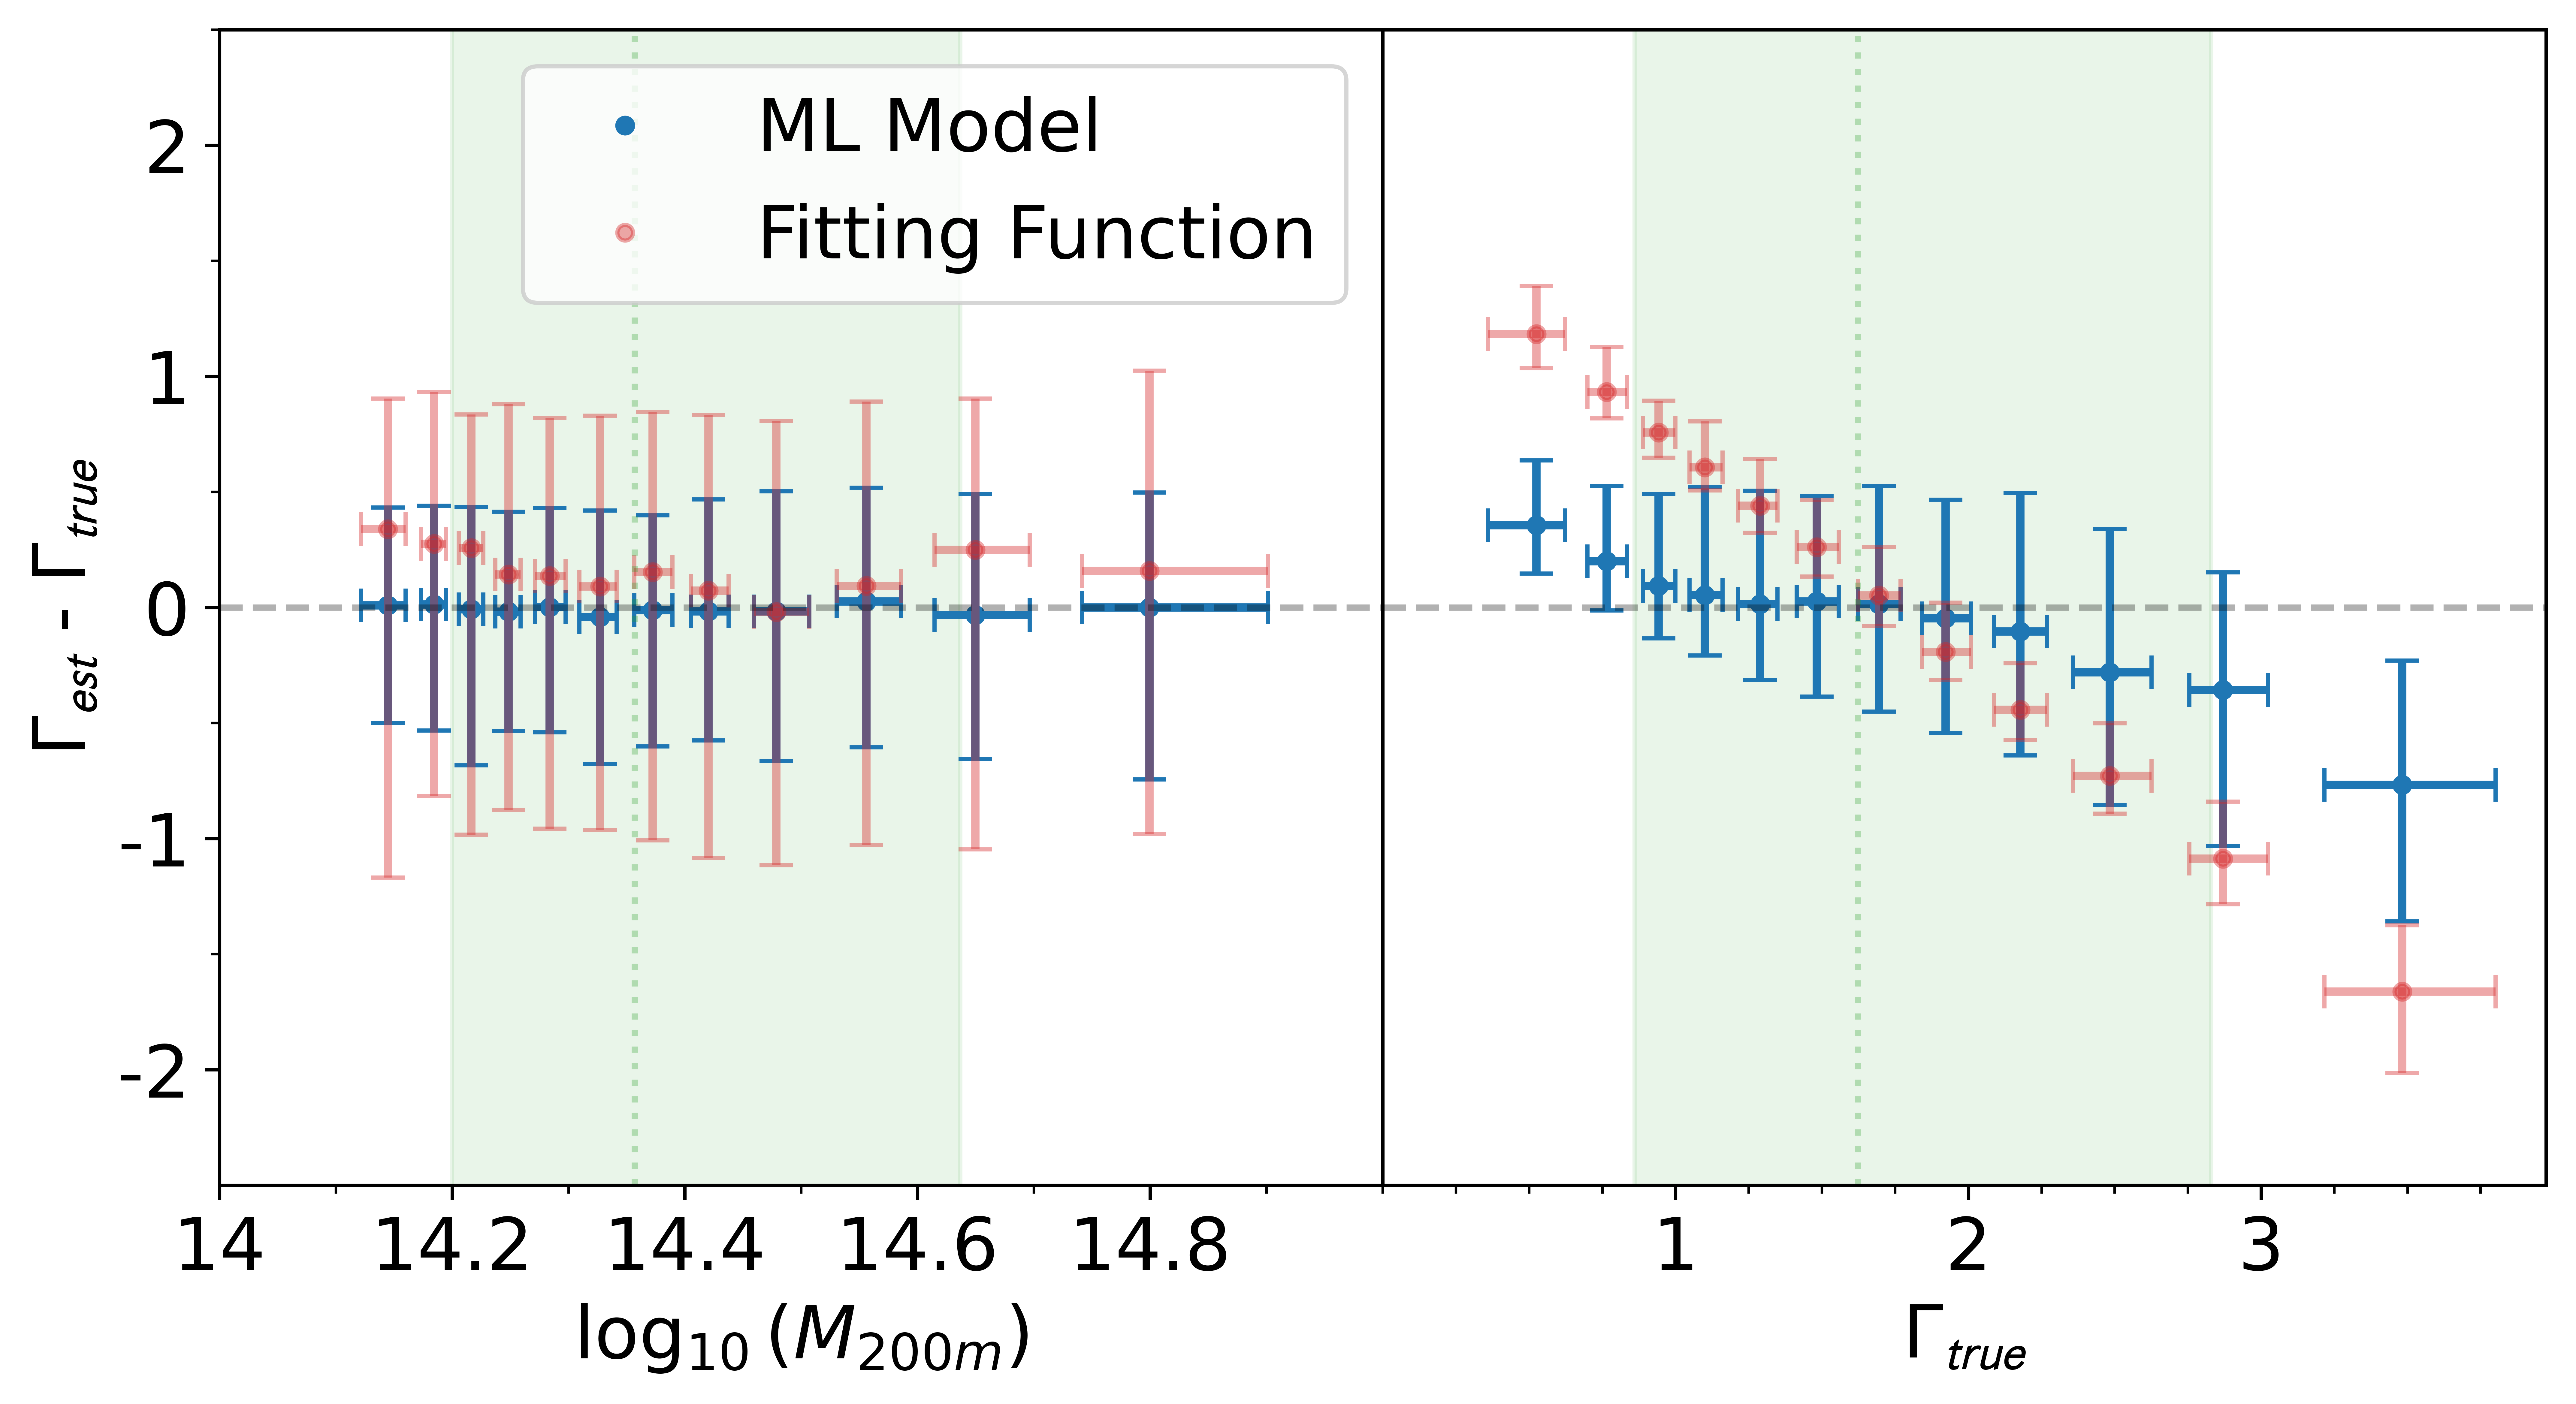
\includegraphics[width=\textwidth]{Ch4_MAH_Est/Model_Compare_NF_CNN_SPM_MW_all_folds_32x32_Prediction_vs_Mass_and_MAR_SIMPLIFIED_091624.png}
    \caption{\raggedright Error bar plots comparing the ML model (blue) to the fitting function (red). All bins contain an equal number of clusters, with horizontal error bars showing the region within which 68\% of the clusters fall, and vertical error bars showing where 68\% of the errors fall (in units of $\Gamma$). The ML model displays no visible bias (points offset from the horizontal dashed line) as a function of galaxy cluster mass (left plot). The ML model is biased as a function of $\Gamma$ (right plot), but less so than the base line model. The bias increases as the cluster MAR strays from the median dataset MAR (vertical dotted line) and the region in which 68\% of the data falls (green shaded region). This bias is likely the result of the unbalanced training data, which contains few examples of very low or high MAR clusters.}
    \label{fig:mass_mar_bias}
\end{figure*}

\subsection{Robustness to Data and Model Variants}\label{Ch4_data_robustness}
While testing our model, we explored a variety of different input data formats (e.g., changes to the input observations). All of these changes had a minimal or negative impact on model performance. In addition to using \textit{Chandra}-like observations, we experimented with more idealized versions of X-ray observations. These idealized mock X-ray observations were surface brightness maps constructed directly from the simulations using the same emission model as the {\it Chandra}-like mocks. These were still split along the same energy bands but lacked any noise, background, or instrument response (unlike the \textit{Chandra}-like mocks). We found only minor improvements in the performance of the model. We also experimented with different image sizes (64x64 and 128x128), but found that no performance was lost when reducing to a smaller size, so we chose a smaller size to reduce computational demands. We believe that this consistency in accuracy across image sizes suggests that we do not have enough unique clusters in our dataset to fully exploit the relationship between small-scale features and MAR. We experimented with multiple different normalizations of the image data (see Equation \ref{eqn:norm}). In one variant, we removed the $tanh()$ function and in another we used a spline function to transform the pixel intensity distribution into a uniform distribution from 0 to 1. Neither of these normalizations improved model performance. 

When using a field-of-view that is fixed in physical size, it is possible for the ML model to learn something about the size of the cluster from its physical extent in the image. To test whether this was essential for estimating the MAR, we trained a model on fields-of-view that scaled depending on different definitions of the physical radius of galaxy clusters ($R_{500c}$, $R_{200m}$). We did not change the size of the images (all were 32x32). Models trained and tested on radius-dependent fields-of-view performed similarly to the fixed field-of-view model. When testing a model, trained on one field-of-view, on test data with a different field-of-view, the model accuracy breaks down, and estimates are no longer usable. When a model is trained on multiple fields-of-view simultaneously and then tested on those fields-of-view, the model achieves a similar accuracy on each field-of-view as the models analyzed in Section~\ref{Ch4_accuracy}, but training is less stable and uncertainties provided by the model are more severely underestimated. Moreover, training on multiple fields-of-view simultaneously results in a larger training set, thereby increasing the computational cost. Consistent accuracy across models trained with different field-of-view images suggests that the necessary information for MAR determination exists at many length scales and radial distances from the core, or that the important information is primarily global, and that the model is not simply using the physical extent of the cluster to constrain MAR.

We also experimented with model variants. In particular, we were interested in the impacts of changing the size of the latent space that connects the CNN and normalizing flows components of the model. We found that increasing the latent space to 5 or 10 variables did not result in a significant change in the performance of the model. Factor of two changes to the size of the model (i.e., the number of weights and CNN filters) did not result in any substantial changes in model performance. Since increasing the model size increased the computational demands for training the model without improving performance, we opted for the aforementioned model architecture.

\section{Image Decomposition \& Interpretation}\label{Ch4_interpretation}

\begin{figure*}[h]%[b]
    \centering
    %\null \vspace{-5pt}
    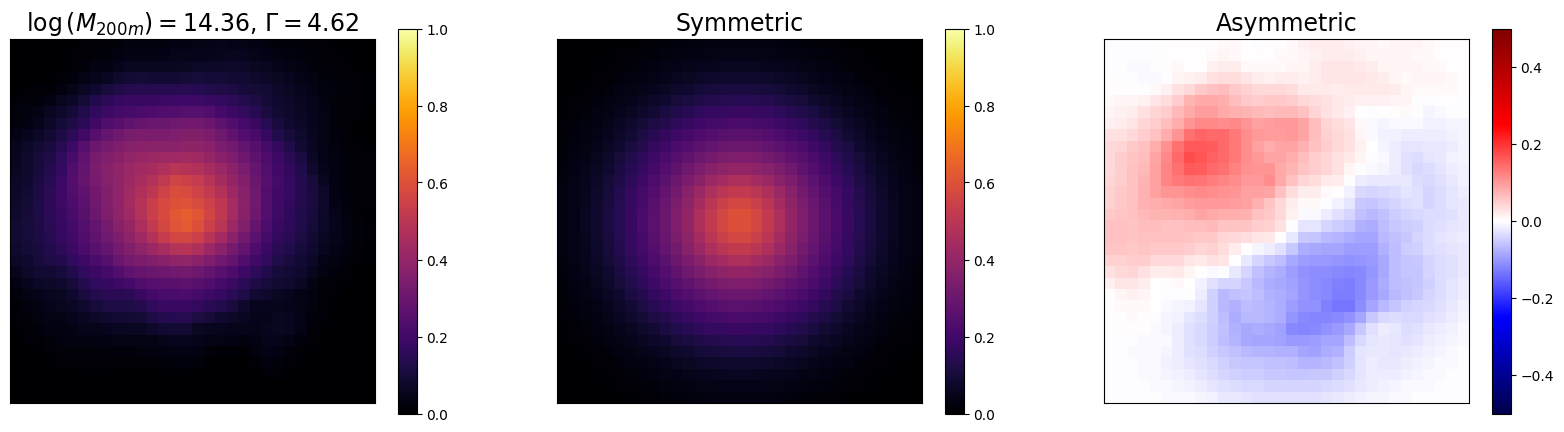
\includegraphics[width=\textwidth]{Ch4_MAH_Est/image_decomp_example_plots_high_mar_tSZ.png}
    \caption{\raggedright A mock tSZ observation of a high MAR galaxy cluster (left) decomposed into symmetric (center) and asymmetric (right) components. The image decomposition technique, discussed in Section~\ref{Ch4_interpretation}, splits images into radially symmetric and asymmetric components. Using this technique  we analyze the relative importance of the radial density profile and the asymmetry of the cluster for MAR estimates.}
    \label{fig:image_decomp_example}
\end{figure*}


We expect the MAR to influence the morphology of galaxy clusters in different ways. From \cite{Diemer_2014} we know that MAR influences the radial density profile of the cluster. However, we also expect that the MAR influences the ellipticity and the fraction of mass contained in the substructure \cite[e.g.,][]{Wong_2012, Jiang_2016}. While our images are very low resolution, all of these pieces of information are present to some degree. To better understand what features in the image influence model estimates, we decompose each cluster into two components, a radially symmetric component and an asymmetric component. The radially symmetric component isolates the importance of the radial density profile of the cluster in MAR determination. The asymmetry component contains a combination of substructure and ellipticity information. By studying the dependence of model estimates on changes in the asymmetric and symmetric components, we hope to better understand the relationship between MAR and the features the components represent.

To decompose the images, we first calculate a radial profile of each image using a one-dimensional Gaussian density kernel with a standard deviation of 0.6. We chose a smoothing factor that was smaller than a single pixel to avoid excessively distorting the true profile. We then correct for pixelation-related artifacts in the profile by dividing by the radial profile of a $32\times32$ matrix of ones\footnote{We know that the profile of an image of ones must be one, therefore any deviation from one is a pixelation error. Dividing by this uncorrected profile removes these pixelation-related errors.}. We used the corrected radial profile to construct a two-dimensional image, calculating the value of each pixel using its distance from the center of the image. The asymmetric image component is the original image minus the symmetric image. We do this calculation for all observation modes and do so on only normalized images. An example of this procedure is shown in Figure \ref{fig:image_decomp_example}.

\begin{figure*}[h]%[b]
    \centering
    %\null \vspace{-5pt}
    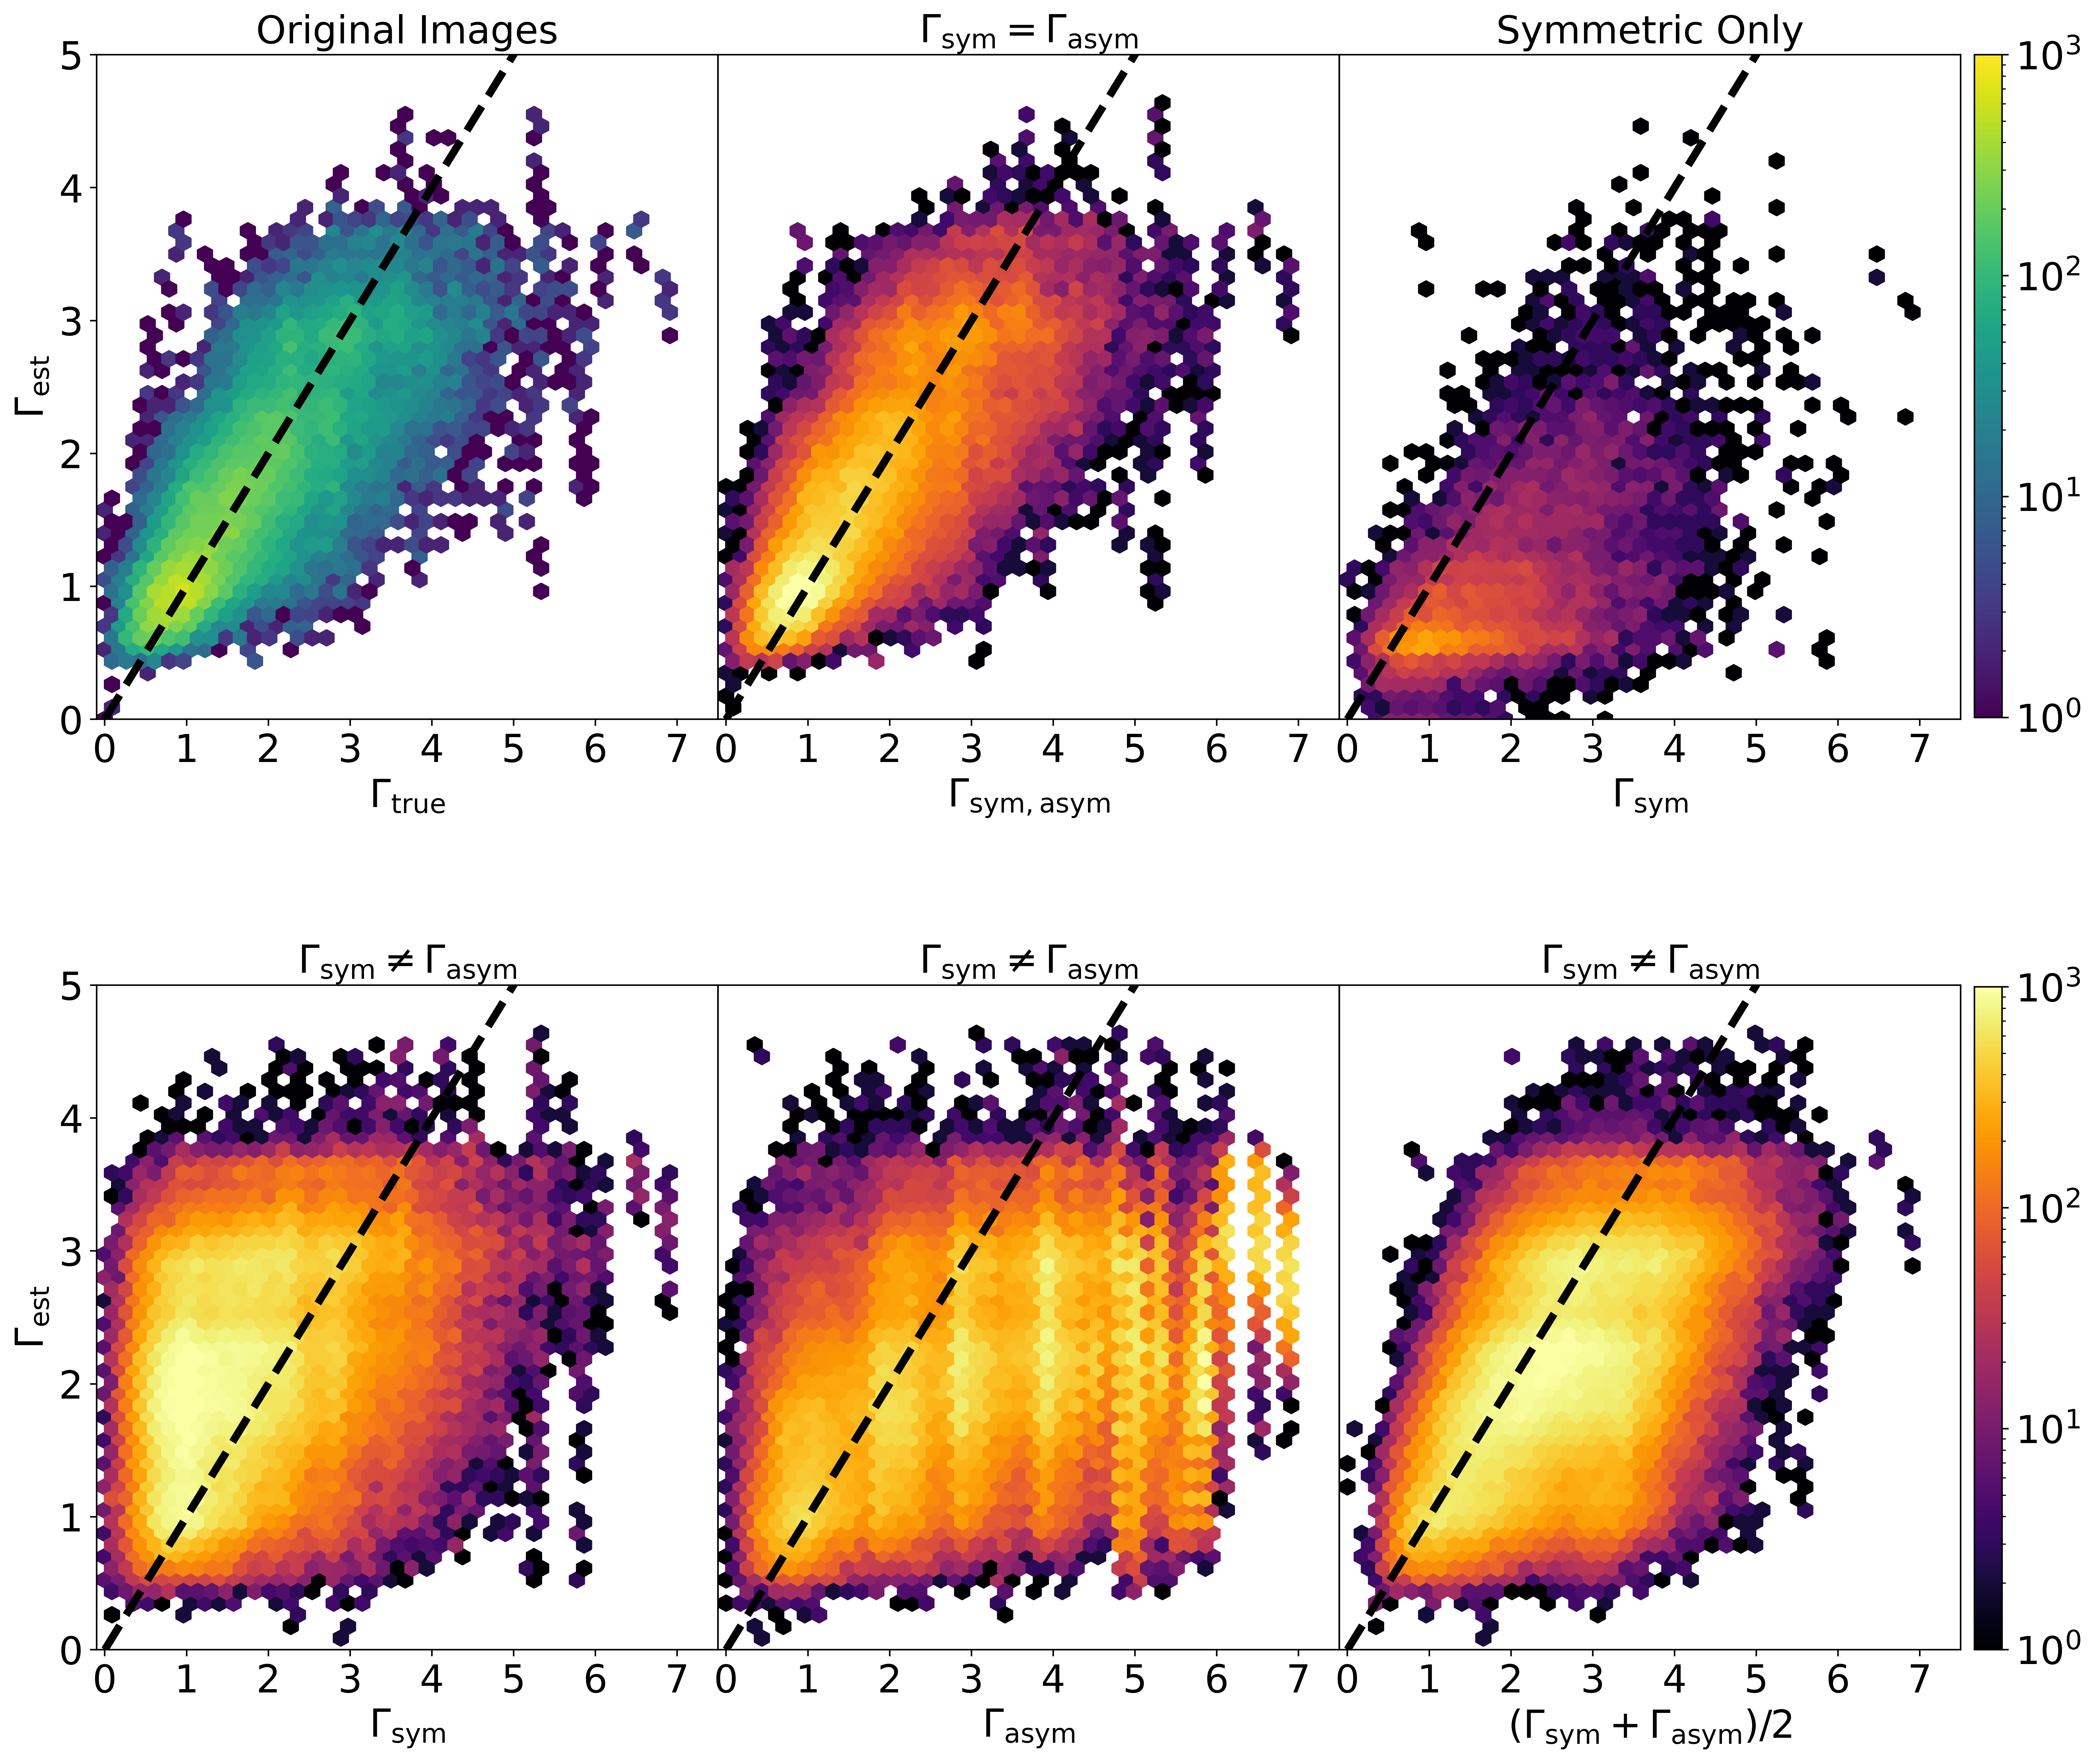
\includegraphics[width=\textwidth]{Ch4_MAH_Est/Symmetric+Asymmetric_Correlations_Mock_Xray_tSZ_fov_39.png}
    \caption{\raggedright 2d histograms of the estimated MARs vs true MARs for different combinations of radially symmetric and asymmetric components. The top left plot, shown with its own color mapping, is the models performance on the unmodified mock observations. The model accuracy is not greatly diminished by combining asymmetric and symmetric components from different lines-of-sight of the same cluster (top center as compared to top left, $\Gamma_{sym} = \Gamma_{asym}$ denotes that both components were calculated from observations of the same cluster). The top right plot shows the model performance when shown only the symmetric components, which results in a persistent underestimate of MAR, suggesting the asymmetric image component is essential to model estimates. When different clusters' components are combined, the MAR estimated is not strongly correlated with the symmetric component (bottom left) or the asymmetric component (bottom center). The correlation between estimates and the average of the MARs of the symmetric and asymmetric components again suggests that both components are essential.}
    \label{fig:symmetric_vs_asymmetric}
\end{figure*}

In our first test, we combined only symmetric and asymmetric components of the same cluster. The radial profile and the asymmetric component of a cluster change depending on the line-of-sight. By mixing and matching the lines-of-sight of the same cluster, we can test how sensitive the model is to these changes. The results of our test are shown in the top center plot of Figure \ref{fig:symmetric_vs_asymmetric}. Using our X-ray and tSZ combined model, we find that the MAR estimates are nearly as accurate as when the original images were used. Using the same accuracy metric as in Section~\ref{Ch4_accuracy}, median estimate percent error percentiles, we find the bounds on the percent errors for 50\%, 68\%, and 95\% of the data are 22\%, 34\%, and 94\%. These results are nearly identical to the model applied to unmodified observations, which strongly suggests that the model is not using information that requires both the symmetric and asymmetric components to have the same line-of-sight. The differences in the radial profiles of a cluster across different lines-of-sight, which are smaller than differences in radial profiles between clusters, are likely to be too small to impact model performance.


In our second test, we use only symmetric inputs. This test allows us to isolate if the model is using asymmetric components at all, and if so, what impact their presence has on model estimates. Naively, we would assume that a radially symmetric cluster is relaxed and therefore has a lower MAR than one with apparent asymmetries. This is indeed what we find, which can be seen in the top right plot of Figure \ref{fig:symmetric_vs_asymmetric}. The model systematically underestimates the MAR of clusters when given only their symmetric components. This suggests that the model uses the asymmetric components, which contain both ellipticity and substructure information. This was further explored by training and testing versions of the model on the symmetric and asymmetric components separately. The results suggest that both the symmetric and asymmetric components contain sufficient information to estimate MAR, but that the accuracy achieved by the model presented requires information from both components.

In our third test, we combine the symmetric and asymmetric components of different clusters of similar mass to create artificial clusters. We then input these artificial clusters into the ML model and obtain MAR estimates for each. We can compare this MAR estimate to the MAR of the cluster used to produce the symmetric component and to the MAR of the cluster used to produce the asymmetric component. The goal of this test is two-fold. Firstly, to determine whether the symmetric component or asymmetric component is dominant in influencing the ML model's MAR estimate. Secondly, to determine whether there is unique information contained in the union of the symmetric and asymmetric components from the same cluster that is lost when these components are mismatched with components of other clusters.

For this test, we separated the clusters into logarithmically spaced mass bins, going from $\log M_{200m} = 14$ to $\log M_{200m} = 16$ in steps of $\Delta\log M_{200m} = 0.25$. We only combined components from clusters that fell within the same mass bin. We did this so that the total size of the cluster in the image would roughly match. We also binned the clusters by their MAR, going from $\Gamma = 0$ to $\Gamma 
 = 7$ in steps of $\Delta \Gamma = 1$. We added the symmetric component of each cluster to the asymmetric component of a different cluster within the same mass bin. We repeated this seven times, so that each cluster was combined with another cluster from the same mass bin and from each of the seven MAR bins. We then compared the predictions of the ML model with the true MAR of the cluster seen in the symmetric component, the true MAR seen in the asymmetric component, and the average of the true MARs of the clusters in both components. The results of the test for mismatched components are shown in the bottom row of Figure \ref{fig:symmetric_vs_asymmetric}. MAR estimates produced by the model are not strongly correlated with either the symmetric or asymmetric component. Comparing the averages of the symmetric and asymmetric MAR improves the correlation somewhat, but not significantly.

 Our third test allows us to see the impact of the MAR of the asymmetric component, controlling for the mass and the MAR of the symmetric component. We find that there is a small mild positive correlation between $\Gamma_{\rm est} - \Gamma_{\rm sym}$ and $\Gamma_{\rm asym} - \Gamma_{\rm sym}$, where $\Gamma_{\rm est}$ is the MAR of the model, $\Gamma_{\rm sym}$ is the MAR of the symmetric component cluster, and $\Gamma_{\rm asym}$ is the MAR of the asymmetric component cluster. In other words, the model estimates a higher MAR relative to the MAR of the symmetric component when a higher MAR asymmetric component is added (and vice versa). This trend is strongest for low-mass clusters and low-MAR symmetric components, but is mild even in the strongest cases. The weakness of the trend suggests that there is important information contained in the union of the symmetric and asymmetric components that is lost when the cluster components are mixed. This is further confirmed by the high scatter relationship between $\Gamma_{\rm est}$ and $\Gamma_{\rm sym}$ when $\Gamma_{\rm asym} \simeq \Gamma_{\rm sym}$.

\section{Conclusion}\label{Ch4_conclusion}
We have developed a MAR estimation technique that uses X-ray and tSZ observations, in combination or individually, to constrain the MAR of mock-observed clusters. This ML model is nearly a factor of two more precise than mass-based estimates, the next best available technique. The presented model demonstrates that important MAR constraining information exists within idealized X-ray and tSZ observations of galaxy clusters. Further work is necessary to demonstrate that such a model can constrain MAR using realistic observations of galaxy clusters as available in the present day. Our mock observations rely on simplifying assumptions, and applying this method to real cluster observations will introduce further challenges. Our model was trained using a single hydrodynamic cosmological simulation, with a single set of assumptions about astrophysics (e.g., AGN feedback) and cosmology. A future model applied to real data will need to be trained on simulated observations with varying astrophysical and cosmological assumptions to reduce the dependence of MAR estimates on these assumptions. Furthermore, our simulated clusters are all observed at the same point in time ($z=0$) and from the same distance ($z=0.05$). A more realistic data set will need to include galaxy clusters observed at different redshifts, to capture differences in structure formation and in foreground (including foreground clusters and filaments). Furthermore, a future model will need to use more realistic observations, perhaps mimicking potential future X-ray experiments (e.g., the Line Emission Mapper\footnote{\url{https://www.lem-observatory.org/}} and Athena\footnote{\url{https://www.the-athena-x-ray-observatory.eu}}). Future work might also explore the benefits of incorporating additional observation modes (e.g., optical, spectral, weak lensing, and radio observations), as well as modifying the ML model architecture. Previous work \cite{Ho_2023}, demonstrates that multiwavelength ML models applied to galaxy clusters are both possible and effective. \cite{Ho_2023} found that combining spectroscopic and X-ray observation information improved their ML models ability to constrain galaxy cluster mass. While inclusion of realistic noise and foreground information may degrade model performance, including additional observation modes may provide unique constraining information not present in the X-ray or tSZ that will improve model performance. Incorporating these changes will require additional data, model retraining, and will likely change the ML models accuracy. To learn what impact these changes have on model accuracy will require substantial analysis. Nevertheless, in this work we demonstrate that a ML model is capable of estimating MAR from idealized observations. This is an essential first step towards building a model capable of estimating the MAR of galaxy clusters from real observations.

Interpreting neural networks is difficult, but we are able to learn useful information in doing so. We verify that our model does not simply use the mass information of the cluster to constrain MAR, as that information is insufficient to achieve our model accuracy. Similarly, experimenting with different fields-of-view confirms that MAR information exists across different length scales and radii. Decomposing images into symmetric and asymmetric components indicates that both the cluster profile and cluster asymmetry are essential to obtain the level of accuracy of our model. The radial profile alone, if used to produce a radially symmetric image, will lead to an underestimate of the MAR. Moreover, there is important information contained in the union of the symmetric and asymmetric components that is essential to our model's performance.

Galaxy cluster MARs must be better understood if we are to answer crucial questions about galaxy cluster physics, improve galaxy cluster mass count constraints of cosmology, or create a new probe of cosmology using MARs. Our ML model, which combines a CNN embedding network with a normalizing flows model, is capable of estimating the MAR of clusters nearly a factor-of-two better than using mass to estimate MAR, while also simultaneously providing an estimate of the uncertainty on those constraints. Further work on directly constraining galaxy cluster MAR offers a promising route towards understanding the galaxy cluster mass bias, improving cosmological parameter constraints derived from galaxy clusters, and enhancing our understanding of the astrophysics that govern the internal dynamics of galaxy clusters.



\section*{Acknowledgments}
We thank Matthew Ho, Arya Farahi, Philip Mansfield, Tibor Rothschild, Ismael Mendoza, Frank van den Bosch, Naomi Gluck, and Priyamvada Natarajan for conversations, questions, and suggestions that led to improvements in this work. 
The material presented is based on work supported by NASA under award No. 80NSSC22K0821.  This work was carried out at the Advanced Research Computing at Hopkins (ARCH) core facility  (rockfish.jhu.edu), which is supported by the National Science Foundation (NSF) grant number OAC 1920103. Ana Maria Delgado acknowledges support from NSF grant number 2307070. CH-A acknowledges support from the Excellence Cluster ORIGINS funded by
the Deutsche Forschungsgemeinschaft (DFG, German Research Foundation)
under Germany's Excellence Strategy -- EXC-2094 -- 390783311. SB acknowledges funding from a UK Research \& Innovation (UKRI) Future Leaders Fellowship [grant number MR/V023381/1]. 

\chapter{Conclusion} \label{chap:chap-5}


%% remove the following and add your chapter text here


%% add more main text technical chapters if you have

%%%%%%%%%%%%%%%%%%%%%%%%%%% END MAIN MATTER %%%%%%%%%%%%%%%%%%%%%%%%%%%%



%%%%%%%%%%%%%%%%%%%%%%%%%%%%% BACK MATTER %%%%%%%%%%%%%%%%%%%%%%%%%%%%%%

%%%% BIBLIOGRAPHIC REFERENCES
\BibTextSpacing                         % text spacing for each bib item
\fancyhead[L]{\nouppercase \leftmark}
\printbibliography[title={Bibliography}, heading=bibintoc, notcategory=mypapers]
\clearpage                              % flushes out floating header


%%%% Appendix chapter (same header format as the main chapters)
%% if you do not have appendix chapters, then comment them out
\MainTextSpacing                    
\fancyhead[L]{\appendixname\ \thechapter. \nouppercase \leftmark}


\include{11-appendix-A}
\include{12-appendix-B}

%% add more appendix chapters if you have 

%%%%%%%%%%%%%%%%%%%%%%%%%%% END BACK MATTER %%%%%%%%%%%%%%%%%%%%%%%%%%%%

\end{document}

%%%%%%%%%%%%%%%%%%%%%%%%% DOCUMENT ENDS HERE %%%%%%%%%%%%%%%%%%%%%%%%%%%